\documentclass[twoside]{book}

% Packages required by doxygen
\usepackage{fixltx2e}
\usepackage{calc}
\usepackage{doxygen}
\usepackage[export]{adjustbox} % also loads graphicx
\usepackage{graphicx}
\usepackage[utf8]{inputenc}
\usepackage{makeidx}
\usepackage{multicol}
\usepackage{multirow}
\PassOptionsToPackage{warn}{textcomp}
\usepackage{textcomp}
\usepackage[nointegrals]{wasysym}
\usepackage[table]{xcolor}

% Font selection
\usepackage[T1]{fontenc}
\usepackage[scaled=.90]{helvet}
\usepackage{courier}
\usepackage{amssymb}
\usepackage{sectsty}
\renewcommand{\familydefault}{\sfdefault}
\allsectionsfont{%
  \fontseries{bc}\selectfont%
  \color{darkgray}%
}
\renewcommand{\DoxyLabelFont}{%
  \fontseries{bc}\selectfont%
  \color{darkgray}%
}
\newcommand{\+}{\discretionary{\mbox{\scriptsize$\hookleftarrow$}}{}{}}

% Page & text layout
\usepackage{geometry}
\geometry{%
  a4paper,%
  top=2.5cm,%
  bottom=2.5cm,%
  left=2.5cm,%
  right=2.5cm%
}
\tolerance=750
\hfuzz=15pt
\hbadness=750
\setlength{\emergencystretch}{15pt}
\setlength{\parindent}{0cm}
\setlength{\parskip}{3ex plus 2ex minus 2ex}
\makeatletter
\renewcommand{\paragraph}{%
  \@startsection{paragraph}{4}{0ex}{-1.0ex}{1.0ex}{%
    \normalfont\normalsize\bfseries\SS@parafont%
  }%
}
\renewcommand{\subparagraph}{%
  \@startsection{subparagraph}{5}{0ex}{-1.0ex}{1.0ex}{%
    \normalfont\normalsize\bfseries\SS@subparafont%
  }%
}
\makeatother

% Headers & footers
\usepackage{fancyhdr}
\pagestyle{fancyplain}
\fancyhead[LE]{\fancyplain{}{\bfseries\thepage}}
\fancyhead[CE]{\fancyplain{}{}}
\fancyhead[RE]{\fancyplain{}{\bfseries\leftmark}}
\fancyhead[LO]{\fancyplain{}{\bfseries\rightmark}}
\fancyhead[CO]{\fancyplain{}{}}
\fancyhead[RO]{\fancyplain{}{\bfseries\thepage}}
\fancyfoot[LE]{\fancyplain{}{}}
\fancyfoot[CE]{\fancyplain{}{}}
\fancyfoot[RE]{\fancyplain{}{\bfseries\scriptsize Generated by Doxygen }}
\fancyfoot[LO]{\fancyplain{}{\bfseries\scriptsize Generated by Doxygen }}
\fancyfoot[CO]{\fancyplain{}{}}
\fancyfoot[RO]{\fancyplain{}{}}
\renewcommand{\footrulewidth}{0.4pt}
\renewcommand{\chaptermark}[1]{%
  \markboth{#1}{}%
}
\renewcommand{\sectionmark}[1]{%
  \markright{\thesection\ #1}%
}

% Indices & bibliography
\usepackage{natbib}
\usepackage[titles]{tocloft}
\setcounter{tocdepth}{3}
\setcounter{secnumdepth}{5}
\makeindex

% Hyperlinks (required, but should be loaded last)
\usepackage{ifpdf}
\ifpdf
  \usepackage[pdftex,pagebackref=true]{hyperref}
\else
  \usepackage[ps2pdf,pagebackref=true]{hyperref}
\fi
\hypersetup{%
  colorlinks=true,%
  linkcolor=blue,%
  citecolor=blue,%
  unicode%
}

% Custom commands
\newcommand{\clearemptydoublepage}{%
  \newpage{\pagestyle{empty}\cleardoublepage}%
}

\usepackage{caption}
\captionsetup{labelsep=space,justification=centering,font={bf},singlelinecheck=off,skip=4pt,position=top}

%===== C O N T E N T S =====

\begin{document}

% Titlepage & ToC
\hypersetup{pageanchor=false,
             bookmarksnumbered=true,
             pdfencoding=unicode
            }
\pagenumbering{alph}
\begin{titlepage}
\vspace*{7cm}
\begin{center}%
{\Large Artificial Life Simulator }\\
\vspace*{1cm}
{\large Generated by Doxygen 1.8.14}\\
\end{center}
\end{titlepage}
\clearemptydoublepage
\pagenumbering{roman}
\tableofcontents
\clearemptydoublepage
\pagenumbering{arabic}
\hypersetup{pageanchor=true}

%--- Begin generated contents ---
\chapter{Hierarchical Index}
\section{Class Hierarchy}
This inheritance list is sorted roughly, but not completely, alphabetically\+:\begin{DoxyCompactList}
\item \contentsline{section}{Abilities\+Editor}{\pageref{class_abilities_editor}}{}
\item \contentsline{section}{Ability}{\pageref{class_ability}}{}
\item \contentsline{section}{Action}{\pageref{class_action}}{}
\begin{DoxyCompactList}
\item \contentsline{section}{Comm\+Action}{\pageref{class_comm_action}}{}
\item \contentsline{section}{Consume\+From\+Land}{\pageref{class_consume_from_land}}{}
\item \contentsline{section}{Move\+Action}{\pageref{class_move_action}}{}
\item \contentsline{section}{Repro\+Action}{\pageref{class_repro_action}}{}
\end{DoxyCompactList}
\item \contentsline{section}{Action\+Editor}{\pageref{class_action_editor}}{}
\item \contentsline{section}{Action\+Editor\+Abstract}{\pageref{class_action_editor_abstract}}{}
\begin{DoxyCompactList}
\item \contentsline{section}{Comm\+Action\+Editor}{\pageref{class_comm_action_editor}}{}
\item \contentsline{section}{Consume\+From\+Land\+Editor}{\pageref{class_consume_from_land_editor}}{}
\item \contentsline{section}{Move\+Action\+Editor}{\pageref{class_move_action_editor}}{}
\item \contentsline{section}{Repro\+Action\+Editor}{\pageref{class_repro_action_editor}}{}
\end{DoxyCompactList}
\item \contentsline{section}{Activation\+Behavior}{\pageref{interface_activation_behavior}}{}
\begin{DoxyCompactList}
\item \contentsline{section}{Empty\+Activ\+Behavior}{\pageref{class_empty_activ_behavior}}{}
\item \contentsline{section}{Logistic\+Activ\+Behavior}{\pageref{class_logistic_activ_behavior}}{}
\item \contentsline{section}{Logistic\+With\+Neg\+Activ\+Behav}{\pageref{class_logistic_with_neg_activ_behav}}{}
\item \contentsline{section}{Tanh\+Activ\+Behav}{\pageref{class_tanh_activ_behav}}{}
\end{DoxyCompactList}
\item \contentsline{section}{Boost\+Requirement}{\pageref{class_boost_requirement}}{}
\item \contentsline{section}{Comm\+Signal}{\pageref{class_comm_signal}}{}
\item \contentsline{section}{Copier}{\pageref{class_copier}}{}
\item \contentsline{section}{Creature}{\pageref{class_creature}}{}
\item \contentsline{section}{Creature\+Editor}{\pageref{class_creature_editor}}{}
\item \contentsline{section}{Creature\+Resource}{\pageref{class_creature_resource}}{}
\item \contentsline{section}{Eco\+Manager}{\pageref{class_eco_manager}}{}
\item \contentsline{section}{Ecosystem}{\pageref{class_ecosystem}}{}
\item \contentsline{section}{Ecosystem\+Editor}{\pageref{class_ecosystem_editor}}{}
\item \contentsline{section}{Helper\+Validator}{\pageref{class_helper_validator}}{}
\item \contentsline{section}{I\+Ecosystem\+Editor}{\pageref{interface_i_ecosystem_editor}}{}
\item \contentsline{section}{Land}{\pageref{class_land}}{}
\item \contentsline{section}{Land\+Resource\+Editor}{\pageref{class_land_resource_editor}}{}
\item \contentsline{section}{Map\+Editor}{\pageref{class_map_editor}}{}
\item Mono\+Behaviour\begin{DoxyCompactList}
\item \contentsline{section}{Camera\+Positioner}{\pageref{class_camera_positioner}}{}
\item \contentsline{section}{Creat\+Menu\+Behav}{\pageref{class_creat_menu_behav}}{}
\item \contentsline{section}{Eco\+Menu\+Behav}{\pageref{class_eco_menu_behav}}{}
\item \contentsline{section}{Eco\+Menu\+Tester}{\pageref{class_eco_menu_tester}}{}
\item \contentsline{section}{Ecosystem\+Getter}{\pageref{class_ecosystem_getter}}{}
\item \contentsline{section}{Error\+Manager}{\pageref{class_error_manager}}{}
\item \contentsline{section}{Game\+Manager}{\pageref{class_game_manager}}{}
\item \contentsline{section}{L\+R\+Menu\+Behav}{\pageref{class_l_r_menu_behav}}{}
\item \contentsline{section}{Main\+Menu\+Behav}{\pageref{class_main_menu_behav}}{}
\item \contentsline{section}{Sim\+Runner\+Test}{\pageref{class_sim_runner_test}}{}
\item \contentsline{section}{Sim\+Runner\+User}{\pageref{class_sim_runner_user}}{}
\item \contentsline{section}{Texture\+Maker\+Example}{\pageref{class_texture_maker_example}}{}
\item \contentsline{section}{Thread\+Manager}{\pageref{class_thread_manager}}{}
\end{DoxyCompactList}
\item \contentsline{section}{Network}{\pageref{class_network}}{}
\begin{DoxyCompactList}
\item \contentsline{section}{Comm\+Network}{\pageref{class_comm_network}}{}
\item \contentsline{section}{Repro\+Network}{\pageref{class_repro_network}}{}
\end{DoxyCompactList}
\item \contentsline{section}{Network\+Editor}{\pageref{class_network_editor}}{}
\item \contentsline{section}{Node}{\pageref{class_node}}{}
\begin{DoxyCompactList}
\item \contentsline{section}{Bias\+Node}{\pageref{class_bias_node}}{}
\item \contentsline{section}{Comm\+Input\+Node}{\pageref{class_comm_input_node}}{}
\item \contentsline{section}{Inner\+Input\+Node}{\pageref{class_inner_input_node}}{}
\item \contentsline{section}{Memory\+Input\+Node}{\pageref{class_memory_input_node}}{}
\item \contentsline{section}{Non\+Input\+Node}{\pageref{class_non_input_node}}{}
\begin{DoxyCompactList}
\item \contentsline{section}{Output\+Node}{\pageref{class_output_node}}{}
\end{DoxyCompactList}
\item \contentsline{section}{Sensory\+Input\+Node}{\pageref{class_sensory_input_node}}{}
\end{DoxyCompactList}
\item \contentsline{section}{Node\+Editor}{\pageref{class_node_editor}}{}
\item \contentsline{section}{Node\+Editor\+Interface}{\pageref{interface_node_editor_interface}}{}
\begin{DoxyCompactList}
\item \contentsline{section}{Comm\+Node\+Editor}{\pageref{class_comm_node_editor}}{}
\item \contentsline{section}{Inner\+Input\+Node\+Editor}{\pageref{class_inner_input_node_editor}}{}
\item \contentsline{section}{Output\+Node\+Editor}{\pageref{class_output_node_editor}}{}
\item \contentsline{section}{Sensory\+Input\+Node\+Editor}{\pageref{class_sensory_input_node_editor}}{}
\end{DoxyCompactList}
\item \contentsline{section}{Population}{\pageref{class_population}}{}
\item \contentsline{section}{Resource\+Editor}{\pageref{class_resource_editor}}{}
\item \contentsline{section}{Resource\+Store}{\pageref{class_resource_store}}{}
\item \contentsline{section}{Species\+Populator}{\pageref{class_species_populator}}{}
\item \contentsline{section}{Static\+Variables}{\pageref{class_static_variables}}{}
\end{DoxyCompactList}

\chapter{Class Index}
\section{Class List}
Here are the classes, structs, unions and interfaces with brief descriptions\+:\begin{DoxyCompactList}
\item\contentsline{section}{\mbox{\hyperlink{class_abilities_editor}{Abilities\+Editor}} \\*A\+PI for Abilities objects. Modifies tentative\+Abilities variable from \mbox{\hyperlink{class_creature_editor}{Creature\+Editor}} }{\pageref{class_abilities_editor}}{}
\item\contentsline{section}{\mbox{\hyperlink{class_ability}{Ability}} \\*Modifies creature\textquotesingle{}s ability to consume certain resources or attack certain species. Each creature has a specific number of ability points to assign to different abilities. }{\pageref{class_ability}}{}
\item\contentsline{section}{\mbox{\hyperlink{class_action}{Action}} }{\pageref{class_action}}{}
\item\contentsline{section}{\mbox{\hyperlink{class_action_editor}{Action\+Editor}} }{\pageref{class_action_editor}}{}
\item\contentsline{section}{\mbox{\hyperlink{class_action_editor_abstract}{Action\+Editor\+Abstract}} }{\pageref{class_action_editor_abstract}}{}
\item\contentsline{section}{\mbox{\hyperlink{interface_activation_behavior}{Activation\+Behavior}} \\*Interface for objects that implement an activation function. }{\pageref{interface_activation_behavior}}{}
\item\contentsline{section}{\mbox{\hyperlink{class_bias_node}{Bias\+Node}} }{\pageref{class_bias_node}}{}
\item\contentsline{section}{\mbox{\hyperlink{class_boost_requirement}{Boost\+Requirement}} \\*Currently not used. Boost requirements allow for modifications to abilities, thus giving creatures with certain resources an advantage over other creatures. If all creatures are capable of this ability, and have the same boost requirements, they all have the opportunity to gain this advantage. However, it should be noted that the relationship between resources and abilities established here does give certain resources more inherent value than others. }{\pageref{class_boost_requirement}}{}
\item\contentsline{section}{\mbox{\hyperlink{class_camera_positioner}{Camera\+Positioner}} }{\pageref{class_camera_positioner}}{}
\item\contentsline{section}{\mbox{\hyperlink{class_comm_action}{Comm\+Action}} }{\pageref{class_comm_action}}{}
\item\contentsline{section}{\mbox{\hyperlink{class_comm_action_editor}{Comm\+Action\+Editor}} }{\pageref{class_comm_action_editor}}{}
\item\contentsline{section}{\mbox{\hyperlink{class_comm_input_node}{Comm\+Input\+Node}} }{\pageref{class_comm_input_node}}{}
\item\contentsline{section}{\mbox{\hyperlink{class_comm_network}{Comm\+Network}} \\*A network that converts incomming comm signals into action recommendations. A seperate comm network is needed for every neightbor that sends a comm signal. }{\pageref{class_comm_network}}{}
\item\contentsline{section}{\mbox{\hyperlink{class_comm_node_editor}{Comm\+Node\+Editor}} \\*A\+PI for Comm Nodes }{\pageref{class_comm_node_editor}}{}
\item\contentsline{section}{\mbox{\hyperlink{class_comm_signal}{Comm\+Signal}} \\*The comm network must individually process each comm signal stored in the creatures comm\+List, and save the outputs as action recommendations. }{\pageref{class_comm_signal}}{}
\item\contentsline{section}{\mbox{\hyperlink{class_consume_from_land}{Consume\+From\+Land}} }{\pageref{class_consume_from_land}}{}
\item\contentsline{section}{\mbox{\hyperlink{class_consume_from_land_editor}{Consume\+From\+Land\+Editor}} }{\pageref{class_consume_from_land_editor}}{}
\item\contentsline{section}{\mbox{\hyperlink{class_copier}{Copier}} }{\pageref{class_copier}}{}
\item\contentsline{section}{\mbox{\hyperlink{class_creat_menu_behav}{Creat\+Menu\+Behav}} }{\pageref{class_creat_menu_behav}}{}
\item\contentsline{section}{\mbox{\hyperlink{class_creature}{Creature}} \\*Class for storing all data about a creature/agent, including its neural networks, queued actions, stored resources, location and other parameters. }{\pageref{class_creature}}{}
\item\contentsline{section}{\mbox{\hyperlink{class_creature_editor}{Creature\+Editor}} }{\pageref{class_creature_editor}}{}
\item\contentsline{section}{\mbox{\hyperlink{class_creature_resource}{Creature\+Resource}} \\*Resource stored by a creature, and how that resource effects the creature. }{\pageref{class_creature_resource}}{}
\item\contentsline{section}{\mbox{\hyperlink{class_eco_manager}{Eco\+Manager}} }{\pageref{class_eco_manager}}{}
\item\contentsline{section}{\mbox{\hyperlink{class_eco_menu_behav}{Eco\+Menu\+Behav}} }{\pageref{class_eco_menu_behav}}{}
\item\contentsline{section}{\mbox{\hyperlink{class_eco_menu_tester}{Eco\+Menu\+Tester}} }{\pageref{class_eco_menu_tester}}{}
\item\contentsline{section}{\mbox{\hyperlink{class_ecosystem}{Ecosystem}} \\*This class contains all of the data about the state of the ecosystem including the populations, species templates, map, resources, and other general parameters. }{\pageref{class_ecosystem}}{}
\item\contentsline{section}{\mbox{\hyperlink{class_ecosystem_editor}{Ecosystem\+Editor}} \\*A\+PI for alterning ecosystem. }{\pageref{class_ecosystem_editor}}{}
\item\contentsline{section}{\mbox{\hyperlink{class_ecosystem_getter}{Ecosystem\+Getter}} }{\pageref{class_ecosystem_getter}}{}
\item\contentsline{section}{\mbox{\hyperlink{class_empty_activ_behavior}{Empty\+Activ\+Behavior}} \\*No activation function (node simply uses linear combination). }{\pageref{class_empty_activ_behavior}}{}
\item\contentsline{section}{\mbox{\hyperlink{class_error_manager}{Error\+Manager}} }{\pageref{class_error_manager}}{}
\item\contentsline{section}{\mbox{\hyperlink{class_game_manager}{Game\+Manager}} }{\pageref{class_game_manager}}{}
\item\contentsline{section}{\mbox{\hyperlink{class_helper_validator}{Helper\+Validator}} }{\pageref{class_helper_validator}}{}
\item\contentsline{section}{\mbox{\hyperlink{interface_i_ecosystem_editor}{I\+Ecosystem\+Editor}} }{\pageref{interface_i_ecosystem_editor}}{}
\item\contentsline{section}{\mbox{\hyperlink{class_inner_input_node}{Inner\+Input\+Node}} }{\pageref{class_inner_input_node}}{}
\item\contentsline{section}{\mbox{\hyperlink{class_inner_input_node_editor}{Inner\+Input\+Node\+Editor}} \\*A\+PI for Inner\+Input\+Nodes. }{\pageref{class_inner_input_node_editor}}{}
\item\contentsline{section}{\mbox{\hyperlink{class_land}{Land}} \\*Class for storing data about a location on the map. Also facilitates creature\textquotesingle{}s interaction with the environment. }{\pageref{class_land}}{}
\item\contentsline{section}{\mbox{\hyperlink{class_land_resource_editor}{Land\+Resource\+Editor}} \\*Used as interface for generating \mbox{\hyperlink{class_resource_store}{Resource\+Store}} objects. }{\pageref{class_land_resource_editor}}{}
\item\contentsline{section}{\mbox{\hyperlink{class_logistic_activ_behavior}{Logistic\+Activ\+Behavior}} \\*Implements logistic activation function. }{\pageref{class_logistic_activ_behavior}}{}
\item\contentsline{section}{\mbox{\hyperlink{class_logistic_with_neg_activ_behav}{Logistic\+With\+Neg\+Activ\+Behav}} \\*Logistic activation function, but mapped to \mbox{[}-\/1,1\mbox{]} }{\pageref{class_logistic_with_neg_activ_behav}}{}
\item\contentsline{section}{\mbox{\hyperlink{class_l_r_menu_behav}{L\+R\+Menu\+Behav}} }{\pageref{class_l_r_menu_behav}}{}
\item\contentsline{section}{\mbox{\hyperlink{class_main_menu_behav}{Main\+Menu\+Behav}} }{\pageref{class_main_menu_behav}}{}
\item\contentsline{section}{\mbox{\hyperlink{class_map_editor}{Map\+Editor}} \\*A\+PI for editing the map\+: a 2D array of \mbox{\hyperlink{class_land}{Land}} spaces. Used to generate the map, and add resources. }{\pageref{class_map_editor}}{}
\item\contentsline{section}{\mbox{\hyperlink{class_memory_input_node}{Memory\+Input\+Node}} }{\pageref{class_memory_input_node}}{}
\item\contentsline{section}{\mbox{\hyperlink{class_move_action}{Move\+Action}} }{\pageref{class_move_action}}{}
\item\contentsline{section}{\mbox{\hyperlink{class_move_action_editor}{Move\+Action\+Editor}} }{\pageref{class_move_action_editor}}{}
\item\contentsline{section}{\mbox{\hyperlink{class_network}{Network}} \\*A neural network of a creature, which consists of layers of nodes. }{\pageref{class_network}}{}
\item\contentsline{section}{\mbox{\hyperlink{class_network_editor}{Network\+Editor}} \\*A\+PI for \mbox{\hyperlink{class_network}{Network}} objects. Stored by Ecosystem\+Creator. }{\pageref{class_network_editor}}{}
\item\contentsline{section}{\mbox{\hyperlink{class_node}{Node}} \\*Abstract parent class for all \mbox{\hyperlink{class_node}{Node}} types. A \mbox{\hyperlink{class_node}{Node}} represents a node in a creatures neural network. }{\pageref{class_node}}{}
\item\contentsline{section}{\mbox{\hyperlink{class_node_editor}{Node\+Editor}} \\*A\+PI for storing different kinds of specific node creators. ex. -\/ could wrap a Sensory\+Input\+Node\+Creator. Stored by Network\+Creator. }{\pageref{class_node_editor}}{}
\item\contentsline{section}{\mbox{\hyperlink{interface_node_editor_interface}{Node\+Editor\+Interface}} \\*Interface that allows all specific node creator objects to be stored by Node\+Creator class. }{\pageref{interface_node_editor_interface}}{}
\item\contentsline{section}{\mbox{\hyperlink{class_non_input_node}{Non\+Input\+Node}} \\*Encompasses hidden nodes (which use this class directly) and output nodes (which use the \mbox{\hyperlink{class_output_node}{Output\+Node}} class). }{\pageref{class_non_input_node}}{}
\item\contentsline{section}{\mbox{\hyperlink{class_output_node}{Output\+Node}} \\*Maps a the value of the node (as calculated by \mbox{\hyperlink{class_non_input_node}{Non\+Input\+Node}} methods) to an action. }{\pageref{class_output_node}}{}
\item\contentsline{section}{\mbox{\hyperlink{class_output_node_editor}{Output\+Node\+Editor}} \\*A\+PI for Output\+Nodes. }{\pageref{class_output_node_editor}}{}
\item\contentsline{section}{\mbox{\hyperlink{class_population}{Population}} \\*A population stores information about a list of creatures, including it\textquotesingle{}s founder, and initial variation. }{\pageref{class_population}}{}
\item\contentsline{section}{\mbox{\hyperlink{class_repro_action}{Repro\+Action}} }{\pageref{class_repro_action}}{}
\item\contentsline{section}{\mbox{\hyperlink{class_repro_action_editor}{Repro\+Action\+Editor}} }{\pageref{class_repro_action_editor}}{}
\item\contentsline{section}{\mbox{\hyperlink{class_repro_network}{Repro\+Network}} \\*A specific kind of network that decided whether a creature should reproduce. }{\pageref{class_repro_network}}{}
\item\contentsline{section}{\mbox{\hyperlink{class_resource_editor}{Resource\+Editor}} \\*A\+PI for setting resources that creature can store, and how the resource effects the creature. }{\pageref{class_resource_editor}}{}
\item\contentsline{section}{\mbox{\hyperlink{class_resource_store}{Resource\+Store}} \\*Basic unit of a resource to be stored in a \mbox{\hyperlink{class_land}{Land}} object. \mbox{\hyperlink{class_creature}{Creature}} can attempt to consume this resource from the land. }{\pageref{class_resource_store}}{}
\item\contentsline{section}{\mbox{\hyperlink{class_sensory_input_node}{Sensory\+Input\+Node}} }{\pageref{class_sensory_input_node}}{}
\item\contentsline{section}{\mbox{\hyperlink{class_sensory_input_node_editor}{Sensory\+Input\+Node\+Editor}} \\*A\+PI for Sensory\+Input\+Nodes. }{\pageref{class_sensory_input_node_editor}}{}
\item\contentsline{section}{\mbox{\hyperlink{class_sim_runner_test}{Sim\+Runner\+Test}} \\*Class for running simulation. }{\pageref{class_sim_runner_test}}{}
\item\contentsline{section}{\mbox{\hyperlink{class_sim_runner_user}{Sim\+Runner\+User}} \\*Class for running simulation. }{\pageref{class_sim_runner_user}}{}
\item\contentsline{section}{\mbox{\hyperlink{class_species_populator}{Species\+Populator}} \\*Class for using a founder species to generate a population on the map. Wraps \mbox{\hyperlink{class_population}{Population}} class. }{\pageref{class_species_populator}}{}
\item\contentsline{section}{\mbox{\hyperlink{class_static_variables}{Static\+Variables}} }{\pageref{class_static_variables}}{}
\item\contentsline{section}{\mbox{\hyperlink{class_tanh_activ_behav}{Tanh\+Activ\+Behav}} \\*Implements Tanh activation function. }{\pageref{class_tanh_activ_behav}}{}
\item\contentsline{section}{\mbox{\hyperlink{class_texture_maker_example}{Texture\+Maker\+Example}} }{\pageref{class_texture_maker_example}}{}
\item\contentsline{section}{\mbox{\hyperlink{class_thread_manager}{Thread\+Manager}} }{\pageref{class_thread_manager}}{}
\end{DoxyCompactList}

\chapter{File Index}
\section{File List}
Here is a list of all files with brief descriptions\+:\begin{DoxyCompactList}
\item\contentsline{section}{\mbox{\hyperlink{_abilities_editor_8cs}{Abilities\+Editor.\+cs}} }{\pageref{_abilities_editor_8cs}}{}
\item\contentsline{section}{\mbox{\hyperlink{_ability_8cs}{Ability.\+cs}} }{\pageref{_ability_8cs}}{}
\item\contentsline{section}{\mbox{\hyperlink{_action_8cs}{Action.\+cs}} }{\pageref{_action_8cs}}{}
\item\contentsline{section}{\mbox{\hyperlink{_action_editor_8cs}{Action\+Editor.\+cs}} }{\pageref{_action_editor_8cs}}{}
\item\contentsline{section}{\mbox{\hyperlink{_action_editor_abstract_8cs}{Action\+Editor\+Abstract.\+cs}} }{\pageref{_action_editor_abstract_8cs}}{}
\item\contentsline{section}{\mbox{\hyperlink{_activation_behavior_8cs}{Activation\+Behavior.\+cs}} }{\pageref{_activation_behavior_8cs}}{}
\item\contentsline{section}{\mbox{\hyperlink{_bias_node_8cs}{Bias\+Node.\+cs}} }{\pageref{_bias_node_8cs}}{}
\item\contentsline{section}{\mbox{\hyperlink{_boost_requirement_8cs}{Boost\+Requirement.\+cs}} }{\pageref{_boost_requirement_8cs}}{}
\item\contentsline{section}{\mbox{\hyperlink{_camera_positioner_8cs}{Camera\+Positioner.\+cs}} }{\pageref{_camera_positioner_8cs}}{}
\item\contentsline{section}{\mbox{\hyperlink{_comm_action_8cs}{Comm\+Action.\+cs}} }{\pageref{_comm_action_8cs}}{}
\item\contentsline{section}{\mbox{\hyperlink{_comm_action_editor_8cs}{Comm\+Action\+Editor.\+cs}} }{\pageref{_comm_action_editor_8cs}}{}
\item\contentsline{section}{\mbox{\hyperlink{_comm_input_node_8cs}{Comm\+Input\+Node.\+cs}} }{\pageref{_comm_input_node_8cs}}{}
\item\contentsline{section}{\mbox{\hyperlink{_comm_network_8cs}{Comm\+Network.\+cs}} }{\pageref{_comm_network_8cs}}{}
\item\contentsline{section}{\mbox{\hyperlink{_comm_node_editor_8cs}{Comm\+Node\+Editor.\+cs}} }{\pageref{_comm_node_editor_8cs}}{}
\item\contentsline{section}{\mbox{\hyperlink{_comm_signal_8cs}{Comm\+Signal.\+cs}} }{\pageref{_comm_signal_8cs}}{}
\item\contentsline{section}{\mbox{\hyperlink{_consume_from_land_8cs}{Consume\+From\+Land.\+cs}} }{\pageref{_consume_from_land_8cs}}{}
\item\contentsline{section}{\mbox{\hyperlink{_consume_from_land_editor_8cs}{Consume\+From\+Land\+Editor.\+cs}} }{\pageref{_consume_from_land_editor_8cs}}{}
\item\contentsline{section}{\mbox{\hyperlink{_copier_8cs}{Copier.\+cs}} }{\pageref{_copier_8cs}}{}
\item\contentsline{section}{\mbox{\hyperlink{_creat_menu_behav_8cs}{Creat\+Menu\+Behav.\+cs}} }{\pageref{_creat_menu_behav_8cs}}{}
\item\contentsline{section}{\mbox{\hyperlink{_creature_8cs}{Creature.\+cs}} }{\pageref{_creature_8cs}}{}
\item\contentsline{section}{\mbox{\hyperlink{_creature_editor_8cs}{Creature\+Editor.\+cs}} }{\pageref{_creature_editor_8cs}}{}
\item\contentsline{section}{\mbox{\hyperlink{_creature_resource_8cs}{Creature\+Resource.\+cs}} }{\pageref{_creature_resource_8cs}}{}
\item\contentsline{section}{\mbox{\hyperlink{_eco_manager_8cs}{Eco\+Manager.\+cs}} }{\pageref{_eco_manager_8cs}}{}
\item\contentsline{section}{\mbox{\hyperlink{_eco_menu_behav_8cs}{Eco\+Menu\+Behav.\+cs}} }{\pageref{_eco_menu_behav_8cs}}{}
\item\contentsline{section}{\mbox{\hyperlink{_eco_menu_tester_8cs}{Eco\+Menu\+Tester.\+cs}} }{\pageref{_eco_menu_tester_8cs}}{}
\item\contentsline{section}{\mbox{\hyperlink{_ecosystem_8cs}{Ecosystem.\+cs}} }{\pageref{_ecosystem_8cs}}{}
\item\contentsline{section}{\mbox{\hyperlink{_ecosystem_editor_8cs}{Ecosystem\+Editor.\+cs}} }{\pageref{_ecosystem_editor_8cs}}{}
\item\contentsline{section}{\mbox{\hyperlink{_ecosystem_getter_8cs}{Ecosystem\+Getter.\+cs}} }{\pageref{_ecosystem_getter_8cs}}{}
\item\contentsline{section}{\mbox{\hyperlink{_empty_activ_behavior_8cs}{Empty\+Activ\+Behavior.\+cs}} }{\pageref{_empty_activ_behavior_8cs}}{}
\item\contentsline{section}{\mbox{\hyperlink{_error_manager_8cs}{Error\+Manager.\+cs}} }{\pageref{_error_manager_8cs}}{}
\item\contentsline{section}{\mbox{\hyperlink{_game_manager_8cs}{Game\+Manager.\+cs}} }{\pageref{_game_manager_8cs}}{}
\item\contentsline{section}{\mbox{\hyperlink{_helper_validator_8cs}{Helper\+Validator.\+cs}} }{\pageref{_helper_validator_8cs}}{}
\item\contentsline{section}{\mbox{\hyperlink{_i_ecosystem_editor_8cs}{I\+Ecosystem\+Editor.\+cs}} }{\pageref{_i_ecosystem_editor_8cs}}{}
\item\contentsline{section}{\mbox{\hyperlink{_inner_input_node_8cs}{Inner\+Input\+Node.\+cs}} }{\pageref{_inner_input_node_8cs}}{}
\item\contentsline{section}{\mbox{\hyperlink{_inner_input_node_editor_8cs}{Inner\+Input\+Node\+Editor.\+cs}} }{\pageref{_inner_input_node_editor_8cs}}{}
\item\contentsline{section}{\mbox{\hyperlink{_land_8cs}{Land.\+cs}} }{\pageref{_land_8cs}}{}
\item\contentsline{section}{\mbox{\hyperlink{_land_resource_editor_8cs}{Land\+Resource\+Editor.\+cs}} }{\pageref{_land_resource_editor_8cs}}{}
\item\contentsline{section}{\mbox{\hyperlink{_logistic_activ_behavior_8cs}{Logistic\+Activ\+Behavior.\+cs}} }{\pageref{_logistic_activ_behavior_8cs}}{}
\item\contentsline{section}{\mbox{\hyperlink{_logistic_with_neg_activ_behav_8cs}{Logistic\+With\+Neg\+Activ\+Behav.\+cs}} }{\pageref{_logistic_with_neg_activ_behav_8cs}}{}
\item\contentsline{section}{\mbox{\hyperlink{_l_r_menu_behav_8cs}{L\+R\+Menu\+Behav.\+cs}} }{\pageref{_l_r_menu_behav_8cs}}{}
\item\contentsline{section}{\mbox{\hyperlink{_main_menu_behav_8cs}{Main\+Menu\+Behav.\+cs}} }{\pageref{_main_menu_behav_8cs}}{}
\item\contentsline{section}{\mbox{\hyperlink{_map_editor_8cs}{Map\+Editor.\+cs}} }{\pageref{_map_editor_8cs}}{}
\item\contentsline{section}{\mbox{\hyperlink{_memory_input_node_8cs}{Memory\+Input\+Node.\+cs}} }{\pageref{_memory_input_node_8cs}}{}
\item\contentsline{section}{\mbox{\hyperlink{_move_action_8cs}{Move\+Action.\+cs}} }{\pageref{_move_action_8cs}}{}
\item\contentsline{section}{\mbox{\hyperlink{_move_action_editor_8cs}{Move\+Action\+Editor.\+cs}} }{\pageref{_move_action_editor_8cs}}{}
\item\contentsline{section}{\mbox{\hyperlink{_network_8cs}{Network.\+cs}} }{\pageref{_network_8cs}}{}
\item\contentsline{section}{\mbox{\hyperlink{_network_editor_8cs}{Network\+Editor.\+cs}} }{\pageref{_network_editor_8cs}}{}
\item\contentsline{section}{\mbox{\hyperlink{_node_8cs}{Node.\+cs}} }{\pageref{_node_8cs}}{}
\item\contentsline{section}{\mbox{\hyperlink{_node_editor_8cs}{Node\+Editor.\+cs}} }{\pageref{_node_editor_8cs}}{}
\item\contentsline{section}{\mbox{\hyperlink{_node_editor_interface_8cs}{Node\+Editor\+Interface.\+cs}} }{\pageref{_node_editor_interface_8cs}}{}
\item\contentsline{section}{\mbox{\hyperlink{_non_input_node_8cs}{Non\+Input\+Node.\+cs}} }{\pageref{_non_input_node_8cs}}{}
\item\contentsline{section}{\mbox{\hyperlink{_output_node_8cs}{Output\+Node.\+cs}} }{\pageref{_output_node_8cs}}{}
\item\contentsline{section}{\mbox{\hyperlink{_output_node_editor_8cs}{Output\+Node\+Editor.\+cs}} }{\pageref{_output_node_editor_8cs}}{}
\item\contentsline{section}{\mbox{\hyperlink{_population_8cs}{Population.\+cs}} }{\pageref{_population_8cs}}{}
\item\contentsline{section}{\mbox{\hyperlink{_repro_action_8cs}{Repro\+Action.\+cs}} }{\pageref{_repro_action_8cs}}{}
\item\contentsline{section}{\mbox{\hyperlink{_repro_action_editor_8cs}{Repro\+Action\+Editor.\+cs}} }{\pageref{_repro_action_editor_8cs}}{}
\item\contentsline{section}{\mbox{\hyperlink{_repro_network_8cs}{Repro\+Network.\+cs}} }{\pageref{_repro_network_8cs}}{}
\item\contentsline{section}{\mbox{\hyperlink{_resource_editor_8cs}{Resource\+Editor.\+cs}} }{\pageref{_resource_editor_8cs}}{}
\item\contentsline{section}{\mbox{\hyperlink{_resource_store_8cs}{Resource\+Store.\+cs}} }{\pageref{_resource_store_8cs}}{}
\item\contentsline{section}{\mbox{\hyperlink{_sensory_input_node_8cs}{Sensory\+Input\+Node.\+cs}} }{\pageref{_sensory_input_node_8cs}}{}
\item\contentsline{section}{\mbox{\hyperlink{_sensory_input_node_editor_8cs}{Sensory\+Input\+Node\+Editor.\+cs}} }{\pageref{_sensory_input_node_editor_8cs}}{}
\item\contentsline{section}{\mbox{\hyperlink{_sim_runner_test_8cs}{Sim\+Runner\+Test.\+cs}} }{\pageref{_sim_runner_test_8cs}}{}
\item\contentsline{section}{\mbox{\hyperlink{_sim_runner_user_8cs}{Sim\+Runner\+User.\+cs}} }{\pageref{_sim_runner_user_8cs}}{}
\item\contentsline{section}{\mbox{\hyperlink{_species_populator_8cs}{Species\+Populator.\+cs}} }{\pageref{_species_populator_8cs}}{}
\item\contentsline{section}{\mbox{\hyperlink{static_variables_8cs}{static\+Variables.\+cs}} }{\pageref{static_variables_8cs}}{}
\item\contentsline{section}{\mbox{\hyperlink{_tanh_activ_behav_8cs}{Tanh\+Activ\+Behav.\+cs}} }{\pageref{_tanh_activ_behav_8cs}}{}
\item\contentsline{section}{\mbox{\hyperlink{_texture_maker_example_8cs}{Texture\+Maker\+Example.\+cs}} }{\pageref{_texture_maker_example_8cs}}{}
\item\contentsline{section}{\mbox{\hyperlink{_thread_manager_8cs}{Thread\+Manager.\+cs}} }{\pageref{_thread_manager_8cs}}{}
\end{DoxyCompactList}

\chapter{Class Documentation}
\hypertarget{class_abilities_editor}{}\section{Abilities\+Editor Class Reference}
\label{class_abilities_editor}\index{Abilities\+Editor@{Abilities\+Editor}}


A\+PI for Abilities objects. Modifies tentative\+Abilities variable from \mbox{\hyperlink{class_creature_editor}{Creature\+Editor}}  


\subsection*{Public Member Functions}
\begin{DoxyCompactItemize}
\item 
\mbox{\hyperlink{class_abilities_editor_aaeefe3c664fe012a1649e9d336191766}{Abilities\+Editor}} (Dictionary$<$ string, \mbox{\hyperlink{class_ability}{Ability}} $>$ \+\_\+abilities, int \+\_\+ability\+Points)
\item 
void \mbox{\hyperlink{class_abilities_editor_aa85324dcb2b8c30fa6c31c17fa4e5020}{add\+Ability}} (string target, \mbox{\hyperlink{_abilities_editor_8cs_ae01c380f385ee9eeb03333f20711ab5a}{ability\+Type}} type)
\begin{DoxyCompactList}\small\item\em Adds ability of specific type and target with level 0 and no boost options. \end{DoxyCompactList}\item 
void \mbox{\hyperlink{class_abilities_editor_ac86ded40f4c4184a8761bef47c24c3b1}{increment\+Ability}} (string target)
\begin{DoxyCompactList}\small\item\em Adds one to ability level. \end{DoxyCompactList}\item 
int \mbox{\hyperlink{class_abilities_editor_a8e906d21f62b192257d3ea08a1cc0615}{get\+Ability\+Points}} ()
\end{DoxyCompactItemize}
\subsection*{Public Attributes}
\begin{DoxyCompactItemize}
\item 
Dictionary$<$ string, \mbox{\hyperlink{class_ability}{Ability}} $>$ \mbox{\hyperlink{class_abilities_editor_a27af464d09981394e9dd4f413704c623}{abilities}}
\item 
int \mbox{\hyperlink{class_abilities_editor_ae5617857224baec0dd3a14e218fe25f7}{remaining\+Ability\+Points}}
\end{DoxyCompactItemize}


\subsection{Detailed Description}
A\+PI for Abilities objects. Modifies tentative\+Abilities variable from \mbox{\hyperlink{class_creature_editor}{Creature\+Editor}} 



\subsection{Constructor \& Destructor Documentation}
\mbox{\Hypertarget{class_abilities_editor_aaeefe3c664fe012a1649e9d336191766}\label{class_abilities_editor_aaeefe3c664fe012a1649e9d336191766}} 
\index{Abilities\+Editor@{Abilities\+Editor}!Abilities\+Editor@{Abilities\+Editor}}
\index{Abilities\+Editor@{Abilities\+Editor}!Abilities\+Editor@{Abilities\+Editor}}
\subsubsection{\texorpdfstring{Abilities\+Editor()}{AbilitiesEditor()}}
{\footnotesize\ttfamily Abilities\+Editor.\+Abilities\+Editor (\begin{DoxyParamCaption}\item[{Dictionary$<$ string, \mbox{\hyperlink{class_ability}{Ability}} $>$}]{\+\_\+abilities,  }\item[{int}]{\+\_\+ability\+Points }\end{DoxyParamCaption})}



\subsection{Member Function Documentation}
\mbox{\Hypertarget{class_abilities_editor_aa85324dcb2b8c30fa6c31c17fa4e5020}\label{class_abilities_editor_aa85324dcb2b8c30fa6c31c17fa4e5020}} 
\index{Abilities\+Editor@{Abilities\+Editor}!add\+Ability@{add\+Ability}}
\index{add\+Ability@{add\+Ability}!Abilities\+Editor@{Abilities\+Editor}}
\subsubsection{\texorpdfstring{add\+Ability()}{addAbility()}}
{\footnotesize\ttfamily void Abilities\+Editor.\+add\+Ability (\begin{DoxyParamCaption}\item[{string}]{target,  }\item[{\mbox{\hyperlink{_abilities_editor_8cs_ae01c380f385ee9eeb03333f20711ab5a}{ability\+Type}}}]{type }\end{DoxyParamCaption})}



Adds ability of specific type and target with level 0 and no boost options. 


\begin{DoxyParams}{Parameters}
{\em target} & The resource/species the ability is applied to.\\
\hline
\end{DoxyParams}
\mbox{\Hypertarget{class_abilities_editor_a8e906d21f62b192257d3ea08a1cc0615}\label{class_abilities_editor_a8e906d21f62b192257d3ea08a1cc0615}} 
\index{Abilities\+Editor@{Abilities\+Editor}!get\+Ability\+Points@{get\+Ability\+Points}}
\index{get\+Ability\+Points@{get\+Ability\+Points}!Abilities\+Editor@{Abilities\+Editor}}
\subsubsection{\texorpdfstring{get\+Ability\+Points()}{getAbilityPoints()}}
{\footnotesize\ttfamily int Abilities\+Editor.\+get\+Ability\+Points (\begin{DoxyParamCaption}{ }\end{DoxyParamCaption})}

\mbox{\Hypertarget{class_abilities_editor_ac86ded40f4c4184a8761bef47c24c3b1}\label{class_abilities_editor_ac86ded40f4c4184a8761bef47c24c3b1}} 
\index{Abilities\+Editor@{Abilities\+Editor}!increment\+Ability@{increment\+Ability}}
\index{increment\+Ability@{increment\+Ability}!Abilities\+Editor@{Abilities\+Editor}}
\subsubsection{\texorpdfstring{increment\+Ability()}{incrementAbility()}}
{\footnotesize\ttfamily void Abilities\+Editor.\+increment\+Ability (\begin{DoxyParamCaption}\item[{string}]{target }\end{DoxyParamCaption})}



Adds one to ability level. 


\begin{DoxyParams}{Parameters}
{\em ability} & \mbox{\hyperlink{class_ability}{Ability}} to be incremented.\\
\hline
\end{DoxyParams}


\subsection{Member Data Documentation}
\mbox{\Hypertarget{class_abilities_editor_a27af464d09981394e9dd4f413704c623}\label{class_abilities_editor_a27af464d09981394e9dd4f413704c623}} 
\index{Abilities\+Editor@{Abilities\+Editor}!abilities@{abilities}}
\index{abilities@{abilities}!Abilities\+Editor@{Abilities\+Editor}}
\subsubsection{\texorpdfstring{abilities}{abilities}}
{\footnotesize\ttfamily Dictionary$<$string, \mbox{\hyperlink{class_ability}{Ability}}$>$ Abilities\+Editor.\+abilities}

\mbox{\Hypertarget{class_abilities_editor_ae5617857224baec0dd3a14e218fe25f7}\label{class_abilities_editor_ae5617857224baec0dd3a14e218fe25f7}} 
\index{Abilities\+Editor@{Abilities\+Editor}!remaining\+Ability\+Points@{remaining\+Ability\+Points}}
\index{remaining\+Ability\+Points@{remaining\+Ability\+Points}!Abilities\+Editor@{Abilities\+Editor}}
\subsubsection{\texorpdfstring{remaining\+Ability\+Points}{remainingAbilityPoints}}
{\footnotesize\ttfamily int Abilities\+Editor.\+remaining\+Ability\+Points}



The documentation for this class was generated from the following file\+:\begin{DoxyCompactItemize}
\item 
\mbox{\hyperlink{_abilities_editor_8cs}{Abilities\+Editor.\+cs}}\end{DoxyCompactItemize}

\hypertarget{class_ability}{}\section{Ability Class Reference}
\label{class_ability}\index{Ability@{Ability}}


Modifies creature\textquotesingle{}s ability to consume certain resources or attack certain species. Each creature has a specific number of ability points to assign to different abilities.  


\subsection*{Public Member Functions}
\begin{DoxyCompactItemize}
\item 
\mbox{\hyperlink{class_ability}{Ability}} \mbox{\hyperlink{class_ability_a633ef57f5e0584a5b28317f790300f7a}{get\+Shallow\+Copy}} ()
\end{DoxyCompactItemize}
\subsection*{Public Attributes}
\begin{DoxyCompactItemize}
\item 
string \mbox{\hyperlink{class_ability_ab843637149d1c6cd3c0f7ee482efb083}{target}}
\begin{DoxyCompactList}\small\item\em Name of resource to consume, or species to attack or defend against. \end{DoxyCompactList}\item 
\mbox{\hyperlink{_abilities_editor_8cs_ae01c380f385ee9eeb03333f20711ab5a}{ability\+Type}} \mbox{\hyperlink{class_ability_ae316cfefaa1ac41f5b24c2d1f41cceba}{type}}
\begin{DoxyCompactList}\small\item\em Groups ability into a category for the user to see \end{DoxyCompactList}\item 
int \mbox{\hyperlink{class_ability_ad7432e0f8cd20857bbc8ff8da0f405c6}{level}}
\begin{DoxyCompactList}\small\item\em Strength of ability. (multiplier to increase chances) \end{DoxyCompactList}\item 
List$<$ \mbox{\hyperlink{class_boost_requirement}{Boost\+Requirement}} $>$ \mbox{\hyperlink{class_ability_ab17185b55f3574f64729cb530848bb97}{boost\+Options}} = new List$<$\mbox{\hyperlink{class_boost_requirement}{Boost\+Requirement}}$>$()
\begin{DoxyCompactList}\small\item\em N\+OT IN U\+SE. List of Boost\+Requirements that could give this ability a boost if the resource needs are met. \end{DoxyCompactList}\end{DoxyCompactItemize}


\subsection{Detailed Description}
Modifies creature\textquotesingle{}s ability to consume certain resources or attack certain species. Each creature has a specific number of ability points to assign to different abilities. 



\subsection{Member Function Documentation}
\mbox{\Hypertarget{class_ability_a633ef57f5e0584a5b28317f790300f7a}\label{class_ability_a633ef57f5e0584a5b28317f790300f7a}} 
\index{Ability@{Ability}!get\+Shallow\+Copy@{get\+Shallow\+Copy}}
\index{get\+Shallow\+Copy@{get\+Shallow\+Copy}!Ability@{Ability}}
\subsubsection{\texorpdfstring{get\+Shallow\+Copy()}{getShallowCopy()}}
{\footnotesize\ttfamily \mbox{\hyperlink{class_ability}{Ability}} Ability.\+get\+Shallow\+Copy (\begin{DoxyParamCaption}{ }\end{DoxyParamCaption})}



\subsection{Member Data Documentation}
\mbox{\Hypertarget{class_ability_ab17185b55f3574f64729cb530848bb97}\label{class_ability_ab17185b55f3574f64729cb530848bb97}} 
\index{Ability@{Ability}!boost\+Options@{boost\+Options}}
\index{boost\+Options@{boost\+Options}!Ability@{Ability}}
\subsubsection{\texorpdfstring{boost\+Options}{boostOptions}}
{\footnotesize\ttfamily List$<$\mbox{\hyperlink{class_boost_requirement}{Boost\+Requirement}}$>$ Ability.\+boost\+Options = new List$<$\mbox{\hyperlink{class_boost_requirement}{Boost\+Requirement}}$>$()}



N\+OT IN U\+SE. List of Boost\+Requirements that could give this ability a boost if the resource needs are met. 

\mbox{\Hypertarget{class_ability_ad7432e0f8cd20857bbc8ff8da0f405c6}\label{class_ability_ad7432e0f8cd20857bbc8ff8da0f405c6}} 
\index{Ability@{Ability}!level@{level}}
\index{level@{level}!Ability@{Ability}}
\subsubsection{\texorpdfstring{level}{level}}
{\footnotesize\ttfamily int Ability.\+level}



Strength of ability. (multiplier to increase chances) 

\mbox{\Hypertarget{class_ability_ab843637149d1c6cd3c0f7ee482efb083}\label{class_ability_ab843637149d1c6cd3c0f7ee482efb083}} 
\index{Ability@{Ability}!target@{target}}
\index{target@{target}!Ability@{Ability}}
\subsubsection{\texorpdfstring{target}{target}}
{\footnotesize\ttfamily string Ability.\+target}



Name of resource to consume, or species to attack or defend against. 

\mbox{\Hypertarget{class_ability_ae316cfefaa1ac41f5b24c2d1f41cceba}\label{class_ability_ae316cfefaa1ac41f5b24c2d1f41cceba}} 
\index{Ability@{Ability}!type@{type}}
\index{type@{type}!Ability@{Ability}}
\subsubsection{\texorpdfstring{type}{type}}
{\footnotesize\ttfamily \mbox{\hyperlink{_abilities_editor_8cs_ae01c380f385ee9eeb03333f20711ab5a}{ability\+Type}} Ability.\+type}



Groups ability into a category for the user to see 



The documentation for this class was generated from the following file\+:\begin{DoxyCompactItemize}
\item 
\mbox{\hyperlink{_ability_8cs}{Ability.\+cs}}\end{DoxyCompactItemize}

\hypertarget{class_action}{}\section{Action Class Reference}
\label{class_action}\index{Action@{Action}}
Inheritance diagram for Action\+:\begin{figure}[H]
\begin{center}
\leavevmode
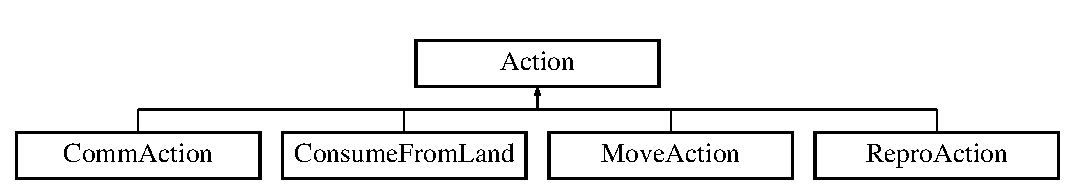
\includegraphics[height=2.000000cm]{class_action}
\end{center}
\end{figure}
\subsection*{Public Member Functions}
\begin{DoxyCompactItemize}
\item 
abstract void \mbox{\hyperlink{class_action_a2aedfc3be16448fbf224cb13607de3c0}{perform}} (\mbox{\hyperlink{class_creature}{Creature}} creature, \mbox{\hyperlink{class_ecosystem}{Ecosystem}} eco)
\item 
void \mbox{\hyperlink{class_action_a1f677dca95b97037f8e0e4bb6b225cb8}{perform\+Wrapper}} (\mbox{\hyperlink{class_creature}{Creature}} c, \mbox{\hyperlink{class_ecosystem}{Ecosystem}} e)
\begin{DoxyCompactList}\small\item\em Performs the action, and spends creatures time and resources \end{DoxyCompactList}\item 
\mbox{\hyperlink{class_action_aed886910937b93b956b61cff7be572bc}{Action}} ()
\item 
bool \mbox{\hyperlink{class_action_a6217cfff19f5f6f7e0638f4dd777864b}{enough\+Resources}} (\mbox{\hyperlink{class_creature}{Creature}} creature)
\item 
void \mbox{\hyperlink{class_action_a4a96d3be0975ce16929ff25f04668189}{spend\+Time\+And\+Resources}} (\mbox{\hyperlink{class_creature}{Creature}} creature)
\item 
\mbox{\hyperlink{class_action}{Action}} \mbox{\hyperlink{class_action_a0c5e2efad9169883c02a215679d0b8be}{get\+Shallow\+Copy}} ()
\end{DoxyCompactItemize}
\subsection*{Public Attributes}
\begin{DoxyCompactItemize}
\item 
string \mbox{\hyperlink{class_action_a3f620f4d21284b95ed2eac1319467747}{name}}
\item 
int \mbox{\hyperlink{class_action_a77b619eb64443ae5f2b729a85a7d7207}{priority}}
\item 
Dictionary$<$ string, int $>$ \mbox{\hyperlink{class_action_afb7d5f622f869e401fcb9edd5961b2fe}{resource\+Costs}} = new Dictionary$<$string, int$>$()
\begin{DoxyCompactList}\small\item\em Stores which resources are spent, and the amount spent \end{DoxyCompactList}\item 
float \mbox{\hyperlink{class_action_a56a4045ce411430256a399031b32ead6}{time\+Cost}}
\item 
int \mbox{\hyperlink{class_action_a04d8b5a2d29dd0b215af21be1a644ac0}{age}}
\end{DoxyCompactItemize}


\subsection{Constructor \& Destructor Documentation}
\mbox{\Hypertarget{class_action_aed886910937b93b956b61cff7be572bc}\label{class_action_aed886910937b93b956b61cff7be572bc}} 
\index{Action@{Action}!Action@{Action}}
\index{Action@{Action}!Action@{Action}}
\subsubsection{\texorpdfstring{Action()}{Action()}}
{\footnotesize\ttfamily Action.\+Action (\begin{DoxyParamCaption}{ }\end{DoxyParamCaption})}



\subsection{Member Function Documentation}
\mbox{\Hypertarget{class_action_a6217cfff19f5f6f7e0638f4dd777864b}\label{class_action_a6217cfff19f5f6f7e0638f4dd777864b}} 
\index{Action@{Action}!enough\+Resources@{enough\+Resources}}
\index{enough\+Resources@{enough\+Resources}!Action@{Action}}
\subsubsection{\texorpdfstring{enough\+Resources()}{enoughResources()}}
{\footnotesize\ttfamily bool Action.\+enough\+Resources (\begin{DoxyParamCaption}\item[{\mbox{\hyperlink{class_creature}{Creature}}}]{creature }\end{DoxyParamCaption})}

\mbox{\Hypertarget{class_action_a0c5e2efad9169883c02a215679d0b8be}\label{class_action_a0c5e2efad9169883c02a215679d0b8be}} 
\index{Action@{Action}!get\+Shallow\+Copy@{get\+Shallow\+Copy}}
\index{get\+Shallow\+Copy@{get\+Shallow\+Copy}!Action@{Action}}
\subsubsection{\texorpdfstring{get\+Shallow\+Copy()}{getShallowCopy()}}
{\footnotesize\ttfamily \mbox{\hyperlink{class_action}{Action}} Action.\+get\+Shallow\+Copy (\begin{DoxyParamCaption}{ }\end{DoxyParamCaption})}

\mbox{\Hypertarget{class_action_a2aedfc3be16448fbf224cb13607de3c0}\label{class_action_a2aedfc3be16448fbf224cb13607de3c0}} 
\index{Action@{Action}!perform@{perform}}
\index{perform@{perform}!Action@{Action}}
\subsubsection{\texorpdfstring{perform()}{perform()}}
{\footnotesize\ttfamily abstract void Action.\+perform (\begin{DoxyParamCaption}\item[{\mbox{\hyperlink{class_creature}{Creature}}}]{creature,  }\item[{\mbox{\hyperlink{class_ecosystem}{Ecosystem}}}]{eco }\end{DoxyParamCaption})\hspace{0.3cm}{\ttfamily [pure virtual]}}



Implemented in \mbox{\hyperlink{class_consume_from_land_a05e266fe8dd4d68b7bec63f53a7f513b}{Consume\+From\+Land}}, \mbox{\hyperlink{class_comm_action_a4ea8e9bcc0a5060221efdc6afefa4355}{Comm\+Action}}, \mbox{\hyperlink{class_move_action_a259b4b4542e7f72df322e060d7737f71}{Move\+Action}}, and \mbox{\hyperlink{class_repro_action_ab018325092d2a13cf333a8576c7f9dd0}{Repro\+Action}}.

\mbox{\Hypertarget{class_action_a1f677dca95b97037f8e0e4bb6b225cb8}\label{class_action_a1f677dca95b97037f8e0e4bb6b225cb8}} 
\index{Action@{Action}!perform\+Wrapper@{perform\+Wrapper}}
\index{perform\+Wrapper@{perform\+Wrapper}!Action@{Action}}
\subsubsection{\texorpdfstring{perform\+Wrapper()}{performWrapper()}}
{\footnotesize\ttfamily void Action.\+perform\+Wrapper (\begin{DoxyParamCaption}\item[{\mbox{\hyperlink{class_creature}{Creature}}}]{c,  }\item[{\mbox{\hyperlink{class_ecosystem}{Ecosystem}}}]{e }\end{DoxyParamCaption})}



Performs the action, and spends creatures time and resources 

\mbox{\Hypertarget{class_action_a4a96d3be0975ce16929ff25f04668189}\label{class_action_a4a96d3be0975ce16929ff25f04668189}} 
\index{Action@{Action}!spend\+Time\+And\+Resources@{spend\+Time\+And\+Resources}}
\index{spend\+Time\+And\+Resources@{spend\+Time\+And\+Resources}!Action@{Action}}
\subsubsection{\texorpdfstring{spend\+Time\+And\+Resources()}{spendTimeAndResources()}}
{\footnotesize\ttfamily void Action.\+spend\+Time\+And\+Resources (\begin{DoxyParamCaption}\item[{\mbox{\hyperlink{class_creature}{Creature}}}]{creature }\end{DoxyParamCaption})}



\subsection{Member Data Documentation}
\mbox{\Hypertarget{class_action_a04d8b5a2d29dd0b215af21be1a644ac0}\label{class_action_a04d8b5a2d29dd0b215af21be1a644ac0}} 
\index{Action@{Action}!age@{age}}
\index{age@{age}!Action@{Action}}
\subsubsection{\texorpdfstring{age}{age}}
{\footnotesize\ttfamily int Action.\+age}

\mbox{\Hypertarget{class_action_a3f620f4d21284b95ed2eac1319467747}\label{class_action_a3f620f4d21284b95ed2eac1319467747}} 
\index{Action@{Action}!name@{name}}
\index{name@{name}!Action@{Action}}
\subsubsection{\texorpdfstring{name}{name}}
{\footnotesize\ttfamily string Action.\+name}

\mbox{\Hypertarget{class_action_a77b619eb64443ae5f2b729a85a7d7207}\label{class_action_a77b619eb64443ae5f2b729a85a7d7207}} 
\index{Action@{Action}!priority@{priority}}
\index{priority@{priority}!Action@{Action}}
\subsubsection{\texorpdfstring{priority}{priority}}
{\footnotesize\ttfamily int Action.\+priority}

\mbox{\Hypertarget{class_action_afb7d5f622f869e401fcb9edd5961b2fe}\label{class_action_afb7d5f622f869e401fcb9edd5961b2fe}} 
\index{Action@{Action}!resource\+Costs@{resource\+Costs}}
\index{resource\+Costs@{resource\+Costs}!Action@{Action}}
\subsubsection{\texorpdfstring{resource\+Costs}{resourceCosts}}
{\footnotesize\ttfamily Dictionary$<$string, int$>$ Action.\+resource\+Costs = new Dictionary$<$string, int$>$()}



Stores which resources are spent, and the amount spent 

\mbox{\Hypertarget{class_action_a56a4045ce411430256a399031b32ead6}\label{class_action_a56a4045ce411430256a399031b32ead6}} 
\index{Action@{Action}!time\+Cost@{time\+Cost}}
\index{time\+Cost@{time\+Cost}!Action@{Action}}
\subsubsection{\texorpdfstring{time\+Cost}{timeCost}}
{\footnotesize\ttfamily float Action.\+time\+Cost}



The documentation for this class was generated from the following file\+:\begin{DoxyCompactItemize}
\item 
\mbox{\hyperlink{_action_8cs}{Action.\+cs}}\end{DoxyCompactItemize}

\hypertarget{class_action_editor}{}\section{Action\+Editor Class Reference}
\label{class_action_editor}\index{Action\+Editor@{Action\+Editor}}
\subsection*{Public Member Functions}
\begin{DoxyCompactItemize}
\item 
\mbox{\hyperlink{class_action_editor_a6ee78410b0b1f863f94d700c971c65ae}{Action\+Editor}} (\mbox{\hyperlink{class_creature_editor}{Creature\+Editor}} cc)
\item 
void \mbox{\hyperlink{class_action_editor_ac134a98ca23fd7c5d95934e9e4d3fd0c}{set\+Creator}} (\mbox{\hyperlink{_action_editor_8cs_a1f6dfc24cb6beb094c3b5a7ad73c805a}{Action\+Creator\+Type}} type)
\item 
\mbox{\hyperlink{class_action_editor_abstract}{Action\+Editor\+Abstract}} \mbox{\hyperlink{class_action_editor_af3bda8deb9bc2b60162102cf681a2cee}{get\+Action\+Creator}} ()
\item 
\mbox{\hyperlink{class_action}{Action}} \mbox{\hyperlink{class_action_editor_a1b9b9e2aaaf5263be088467c0fdc310f}{get\+Created\+Action}} ()
\end{DoxyCompactItemize}


\subsection{Constructor \& Destructor Documentation}
\mbox{\Hypertarget{class_action_editor_a6ee78410b0b1f863f94d700c971c65ae}\label{class_action_editor_a6ee78410b0b1f863f94d700c971c65ae}} 
\index{Action\+Editor@{Action\+Editor}!Action\+Editor@{Action\+Editor}}
\index{Action\+Editor@{Action\+Editor}!Action\+Editor@{Action\+Editor}}
\subsubsection{\texorpdfstring{Action\+Editor()}{ActionEditor()}}
{\footnotesize\ttfamily Action\+Editor.\+Action\+Editor (\begin{DoxyParamCaption}\item[{\mbox{\hyperlink{class_creature_editor}{Creature\+Editor}}}]{cc }\end{DoxyParamCaption})}



\subsection{Member Function Documentation}
\mbox{\Hypertarget{class_action_editor_af3bda8deb9bc2b60162102cf681a2cee}\label{class_action_editor_af3bda8deb9bc2b60162102cf681a2cee}} 
\index{Action\+Editor@{Action\+Editor}!get\+Action\+Creator@{get\+Action\+Creator}}
\index{get\+Action\+Creator@{get\+Action\+Creator}!Action\+Editor@{Action\+Editor}}
\subsubsection{\texorpdfstring{get\+Action\+Creator()}{getActionCreator()}}
{\footnotesize\ttfamily \mbox{\hyperlink{class_action_editor_abstract}{Action\+Editor\+Abstract}} Action\+Editor.\+get\+Action\+Creator (\begin{DoxyParamCaption}{ }\end{DoxyParamCaption})}

\mbox{\Hypertarget{class_action_editor_a1b9b9e2aaaf5263be088467c0fdc310f}\label{class_action_editor_a1b9b9e2aaaf5263be088467c0fdc310f}} 
\index{Action\+Editor@{Action\+Editor}!get\+Created\+Action@{get\+Created\+Action}}
\index{get\+Created\+Action@{get\+Created\+Action}!Action\+Editor@{Action\+Editor}}
\subsubsection{\texorpdfstring{get\+Created\+Action()}{getCreatedAction()}}
{\footnotesize\ttfamily \mbox{\hyperlink{class_action}{Action}} Action\+Editor.\+get\+Created\+Action (\begin{DoxyParamCaption}{ }\end{DoxyParamCaption})}

\mbox{\Hypertarget{class_action_editor_ac134a98ca23fd7c5d95934e9e4d3fd0c}\label{class_action_editor_ac134a98ca23fd7c5d95934e9e4d3fd0c}} 
\index{Action\+Editor@{Action\+Editor}!set\+Creator@{set\+Creator}}
\index{set\+Creator@{set\+Creator}!Action\+Editor@{Action\+Editor}}
\subsubsection{\texorpdfstring{set\+Creator()}{setCreator()}}
{\footnotesize\ttfamily void Action\+Editor.\+set\+Creator (\begin{DoxyParamCaption}\item[{\mbox{\hyperlink{_action_editor_8cs_a1f6dfc24cb6beb094c3b5a7ad73c805a}{Action\+Creator\+Type}}}]{type }\end{DoxyParamCaption})}



The documentation for this class was generated from the following file\+:\begin{DoxyCompactItemize}
\item 
\mbox{\hyperlink{_action_editor_8cs}{Action\+Editor.\+cs}}\end{DoxyCompactItemize}

\hypertarget{class_action_editor_abstract}{}\section{Action\+Editor\+Abstract Class Reference}
\label{class_action_editor_abstract}\index{Action\+Editor\+Abstract@{Action\+Editor\+Abstract}}
Inheritance diagram for Action\+Editor\+Abstract\+:\begin{figure}[H]
\begin{center}
\leavevmode
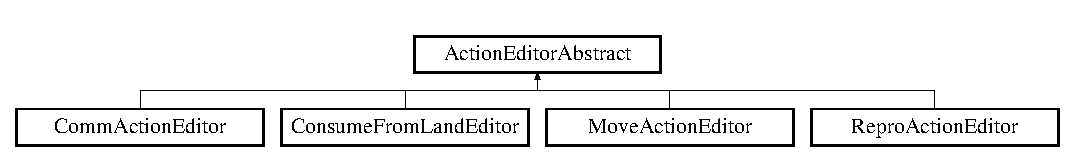
\includegraphics[height=1.728395cm]{class_action_editor_abstract}
\end{center}
\end{figure}
\subsection*{Public Member Functions}
\begin{DoxyCompactItemize}
\item 
\mbox{\hyperlink{class_action}{Action}} \mbox{\hyperlink{class_action_editor_abstract_a7c529d2f6fd2c7db4f8451cb90aabe75}{get\+Action}} ()
\item 
void \mbox{\hyperlink{class_action_editor_abstract_aa6da20f7ed4358957d5c4a0d3b191877}{set\+Time\+Cost}} (int cost)
\item 
void \mbox{\hyperlink{class_action_editor_abstract_a85dfd2bcf2a86bb45c2cafeed4d4b9fc}{add\+Resource\+Cost}} (string key, int value)
\item 
void \mbox{\hyperlink{class_action_editor_abstract_a2b18204979082f6227f55e357cdcc5d5}{set\+Priority}} (int priority)
\item 
void \mbox{\hyperlink{class_action_editor_abstract_a15e82c4d5b251a80396ae635fd1f0fa2}{set\+Name}} (string name)
\end{DoxyCompactItemize}
\subsection*{Public Attributes}
\begin{DoxyCompactItemize}
\item 
\mbox{\hyperlink{class_action}{Action}} \mbox{\hyperlink{class_action_editor_abstract_a58e0f5d65d95e8e4b80a0b3d5e82ce7b}{action}}
\end{DoxyCompactItemize}


\subsection{Member Function Documentation}
\mbox{\Hypertarget{class_action_editor_abstract_a85dfd2bcf2a86bb45c2cafeed4d4b9fc}\label{class_action_editor_abstract_a85dfd2bcf2a86bb45c2cafeed4d4b9fc}} 
\index{Action\+Editor\+Abstract@{Action\+Editor\+Abstract}!add\+Resource\+Cost@{add\+Resource\+Cost}}
\index{add\+Resource\+Cost@{add\+Resource\+Cost}!Action\+Editor\+Abstract@{Action\+Editor\+Abstract}}
\subsubsection{\texorpdfstring{add\+Resource\+Cost()}{addResourceCost()}}
{\footnotesize\ttfamily void Action\+Editor\+Abstract.\+add\+Resource\+Cost (\begin{DoxyParamCaption}\item[{string}]{key,  }\item[{int}]{value }\end{DoxyParamCaption})}

\mbox{\Hypertarget{class_action_editor_abstract_a7c529d2f6fd2c7db4f8451cb90aabe75}\label{class_action_editor_abstract_a7c529d2f6fd2c7db4f8451cb90aabe75}} 
\index{Action\+Editor\+Abstract@{Action\+Editor\+Abstract}!get\+Action@{get\+Action}}
\index{get\+Action@{get\+Action}!Action\+Editor\+Abstract@{Action\+Editor\+Abstract}}
\subsubsection{\texorpdfstring{get\+Action()}{getAction()}}
{\footnotesize\ttfamily \mbox{\hyperlink{class_action}{Action}} Action\+Editor\+Abstract.\+get\+Action (\begin{DoxyParamCaption}{ }\end{DoxyParamCaption})}

\mbox{\Hypertarget{class_action_editor_abstract_a15e82c4d5b251a80396ae635fd1f0fa2}\label{class_action_editor_abstract_a15e82c4d5b251a80396ae635fd1f0fa2}} 
\index{Action\+Editor\+Abstract@{Action\+Editor\+Abstract}!set\+Name@{set\+Name}}
\index{set\+Name@{set\+Name}!Action\+Editor\+Abstract@{Action\+Editor\+Abstract}}
\subsubsection{\texorpdfstring{set\+Name()}{setName()}}
{\footnotesize\ttfamily void Action\+Editor\+Abstract.\+set\+Name (\begin{DoxyParamCaption}\item[{string}]{name }\end{DoxyParamCaption})}

\mbox{\Hypertarget{class_action_editor_abstract_a2b18204979082f6227f55e357cdcc5d5}\label{class_action_editor_abstract_a2b18204979082f6227f55e357cdcc5d5}} 
\index{Action\+Editor\+Abstract@{Action\+Editor\+Abstract}!set\+Priority@{set\+Priority}}
\index{set\+Priority@{set\+Priority}!Action\+Editor\+Abstract@{Action\+Editor\+Abstract}}
\subsubsection{\texorpdfstring{set\+Priority()}{setPriority()}}
{\footnotesize\ttfamily void Action\+Editor\+Abstract.\+set\+Priority (\begin{DoxyParamCaption}\item[{int}]{priority }\end{DoxyParamCaption})}

\mbox{\Hypertarget{class_action_editor_abstract_aa6da20f7ed4358957d5c4a0d3b191877}\label{class_action_editor_abstract_aa6da20f7ed4358957d5c4a0d3b191877}} 
\index{Action\+Editor\+Abstract@{Action\+Editor\+Abstract}!set\+Time\+Cost@{set\+Time\+Cost}}
\index{set\+Time\+Cost@{set\+Time\+Cost}!Action\+Editor\+Abstract@{Action\+Editor\+Abstract}}
\subsubsection{\texorpdfstring{set\+Time\+Cost()}{setTimeCost()}}
{\footnotesize\ttfamily void Action\+Editor\+Abstract.\+set\+Time\+Cost (\begin{DoxyParamCaption}\item[{int}]{cost }\end{DoxyParamCaption})}



\subsection{Member Data Documentation}
\mbox{\Hypertarget{class_action_editor_abstract_a58e0f5d65d95e8e4b80a0b3d5e82ce7b}\label{class_action_editor_abstract_a58e0f5d65d95e8e4b80a0b3d5e82ce7b}} 
\index{Action\+Editor\+Abstract@{Action\+Editor\+Abstract}!action@{action}}
\index{action@{action}!Action\+Editor\+Abstract@{Action\+Editor\+Abstract}}
\subsubsection{\texorpdfstring{action}{action}}
{\footnotesize\ttfamily \mbox{\hyperlink{class_action}{Action}} Action\+Editor\+Abstract.\+action}



The documentation for this class was generated from the following file\+:\begin{DoxyCompactItemize}
\item 
\mbox{\hyperlink{_action_editor_abstract_8cs}{Action\+Editor\+Abstract.\+cs}}\end{DoxyCompactItemize}

\hypertarget{interface_activation_behavior}{}\section{Activation\+Behavior Interface Reference}
\label{interface_activation_behavior}\index{Activation\+Behavior@{Activation\+Behavior}}


Interface for objects that implement an activation function.  


Inheritance diagram for Activation\+Behavior\+:\begin{figure}[H]
\begin{center}
\leavevmode
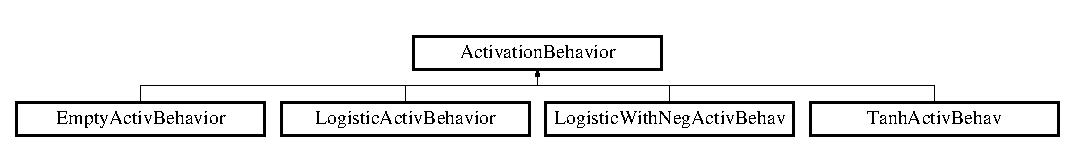
\includegraphics[height=1.600000cm]{interface_activation_behavior}
\end{center}
\end{figure}
\subsection*{Public Member Functions}
\begin{DoxyCompactItemize}
\item 
float \mbox{\hyperlink{interface_activation_behavior_a6c7af51cf1b10eaadcbf086231e5539b}{activ\+Funct}} (float input)
\end{DoxyCompactItemize}


\subsection{Detailed Description}
Interface for objects that implement an activation function. 



\subsection{Member Function Documentation}
\mbox{\Hypertarget{interface_activation_behavior_a6c7af51cf1b10eaadcbf086231e5539b}\label{interface_activation_behavior_a6c7af51cf1b10eaadcbf086231e5539b}} 
\index{Activation\+Behavior@{Activation\+Behavior}!activ\+Funct@{activ\+Funct}}
\index{activ\+Funct@{activ\+Funct}!Activation\+Behavior@{Activation\+Behavior}}
\subsubsection{\texorpdfstring{activ\+Funct()}{activFunct()}}
{\footnotesize\ttfamily float Activation\+Behavior.\+activ\+Funct (\begin{DoxyParamCaption}\item[{float}]{input }\end{DoxyParamCaption})}



Implemented in \mbox{\hyperlink{class_logistic_activ_behavior_a20a20f3e29d8aad19f35067a9304ee96}{Logistic\+Activ\+Behavior}}, \mbox{\hyperlink{class_empty_activ_behavior_acc640ba59f2c258030501f8ec9c537d8}{Empty\+Activ\+Behavior}}, \mbox{\hyperlink{class_logistic_with_neg_activ_behav_abfe284e0e1854e171412cb2e6f0ad8e3}{Logistic\+With\+Neg\+Activ\+Behav}}, and \mbox{\hyperlink{class_tanh_activ_behav_a7aa47f0ab45debc7cc89d62334e28b77}{Tanh\+Activ\+Behav}}.



The documentation for this interface was generated from the following file\+:\begin{DoxyCompactItemize}
\item 
\mbox{\hyperlink{_activation_behavior_8cs}{Activation\+Behavior.\+cs}}\end{DoxyCompactItemize}

\hypertarget{class_bias_node}{}\section{Bias\+Node Class Reference}
\label{class_bias_node}\index{Bias\+Node@{Bias\+Node}}
Inheritance diagram for Bias\+Node\+:\begin{figure}[H]
\begin{center}
\leavevmode
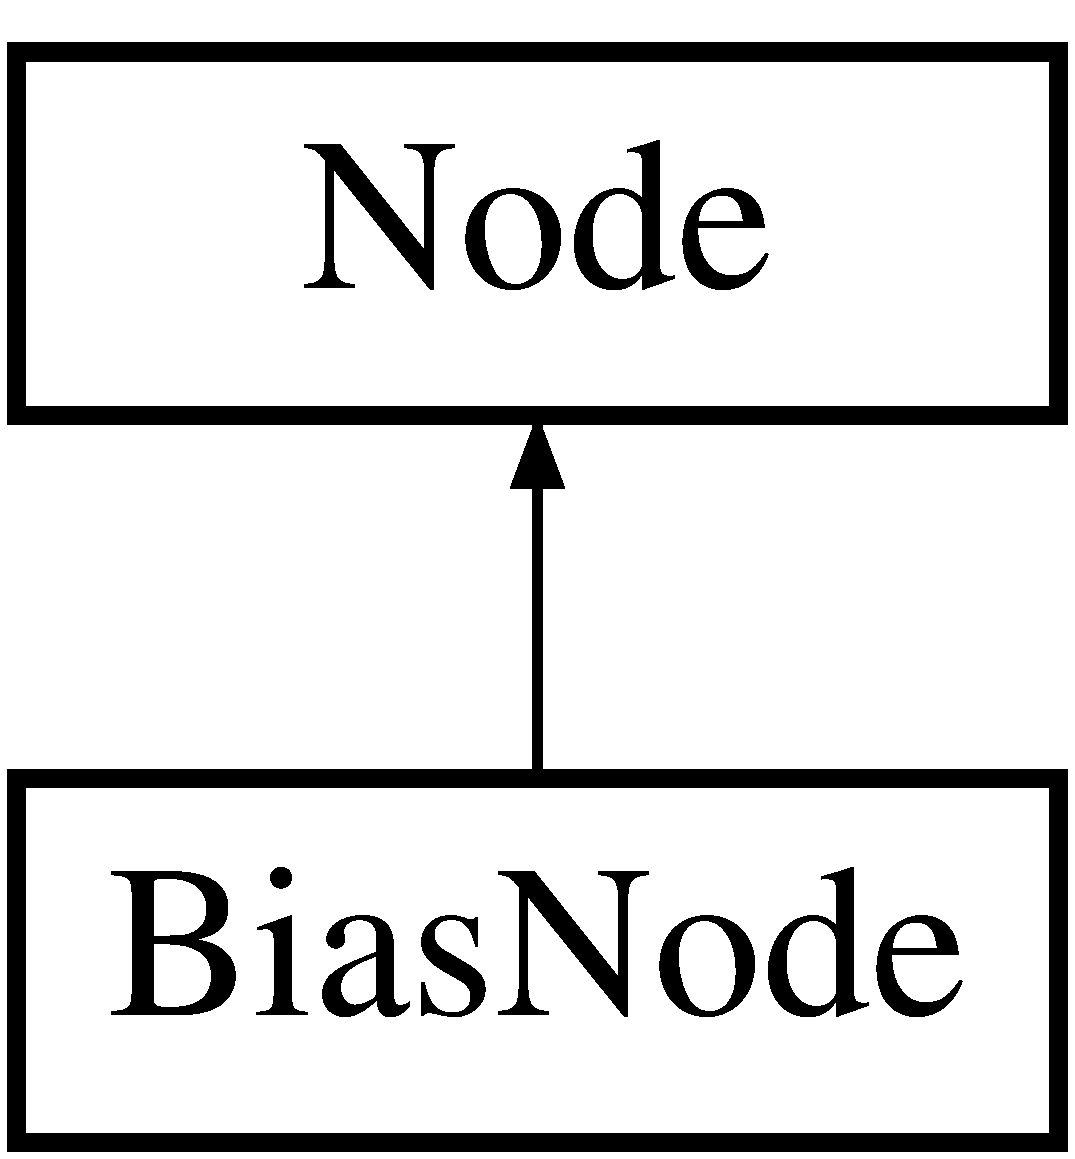
\includegraphics[height=2.000000cm]{class_bias_node}
\end{center}
\end{figure}
\subsection*{Public Member Functions}
\begin{DoxyCompactItemize}
\item 
void \mbox{\hyperlink{class_bias_node_a73832b9f58014cc9f17788ce64f56989}{set\+Bias}} (float new\+Bias)
\begin{DoxyCompactList}\small\item\em sets bias to a value \end{DoxyCompactList}\item 
override void \mbox{\hyperlink{class_bias_node_a84e7e92b97256707aba057ec92bd7a79}{update\+Value}} ()
\begin{DoxyCompactList}\small\item\em Updates node value \end{DoxyCompactList}\item 
\mbox{\hyperlink{class_bias_node}{Bias\+Node}} \mbox{\hyperlink{class_bias_node_aa948061d92ef7e0b8d470a0b6c01b7a1}{clone}} ()
\end{DoxyCompactItemize}
\subsection*{Additional Inherited Members}


\subsection{Member Function Documentation}
\mbox{\Hypertarget{class_bias_node_aa948061d92ef7e0b8d470a0b6c01b7a1}\label{class_bias_node_aa948061d92ef7e0b8d470a0b6c01b7a1}} 
\index{Bias\+Node@{Bias\+Node}!clone@{clone}}
\index{clone@{clone}!Bias\+Node@{Bias\+Node}}
\subsubsection{\texorpdfstring{clone()}{clone()}}
{\footnotesize\ttfamily \mbox{\hyperlink{class_bias_node}{Bias\+Node}} Bias\+Node.\+clone (\begin{DoxyParamCaption}{ }\end{DoxyParamCaption})}

\mbox{\Hypertarget{class_bias_node_a73832b9f58014cc9f17788ce64f56989}\label{class_bias_node_a73832b9f58014cc9f17788ce64f56989}} 
\index{Bias\+Node@{Bias\+Node}!set\+Bias@{set\+Bias}}
\index{set\+Bias@{set\+Bias}!Bias\+Node@{Bias\+Node}}
\subsubsection{\texorpdfstring{set\+Bias()}{setBias()}}
{\footnotesize\ttfamily void Bias\+Node.\+set\+Bias (\begin{DoxyParamCaption}\item[{float}]{new\+Bias }\end{DoxyParamCaption})}



sets bias to a value 

\mbox{\Hypertarget{class_bias_node_a84e7e92b97256707aba057ec92bd7a79}\label{class_bias_node_a84e7e92b97256707aba057ec92bd7a79}} 
\index{Bias\+Node@{Bias\+Node}!update\+Value@{update\+Value}}
\index{update\+Value@{update\+Value}!Bias\+Node@{Bias\+Node}}
\subsubsection{\texorpdfstring{update\+Value()}{updateValue()}}
{\footnotesize\ttfamily override void Bias\+Node.\+update\+Value (\begin{DoxyParamCaption}{ }\end{DoxyParamCaption})\hspace{0.3cm}{\ttfamily [virtual]}}



Updates node value 



Implements \mbox{\hyperlink{class_node_a85ebd0e36c25430570b94f923afd2a62}{Node}}.



The documentation for this class was generated from the following file\+:\begin{DoxyCompactItemize}
\item 
\mbox{\hyperlink{_bias_node_8cs}{Bias\+Node.\+cs}}\end{DoxyCompactItemize}

\hypertarget{class_boost_requirement}{}\section{Boost\+Requirement Class Reference}
\label{class_boost_requirement}\index{Boost\+Requirement@{Boost\+Requirement}}


Currently not used. Boost requirements allow for modifications to abilities, thus giving creatures with certain resources an advantage over other creatures. If all creatures are capable of this ability, and have the same boost requirements, they all have the opportunity to gain this advantage. However, it should be noted that the relationship between resources and abilities established here does give certain resources more inherent value than others.  


\subsection*{Public Member Functions}
\begin{DoxyCompactItemize}
\item 
\mbox{\hyperlink{class_boost_requirement}{Boost\+Requirement}} \mbox{\hyperlink{class_boost_requirement_aebc683969c2561e56a2b45d98d54876d}{get\+Shallow\+Copy}} ()
\end{DoxyCompactItemize}
\subsection*{Public Attributes}
\begin{DoxyCompactItemize}
\item 
Dictionary$<$ string, int $>$ \mbox{\hyperlink{class_boost_requirement_ad0415c1e37d462bffcf3c3e4dbf69eed}{required\+Resources}}
\begin{DoxyCompactList}\small\item\em List of resources required for boost, and their thresholds. \end{DoxyCompactList}\item 
int \mbox{\hyperlink{class_boost_requirement_ace675651f02aff4a40aecc2ab40d4822}{boost\+Amount}}
\begin{DoxyCompactList}\small\item\em The amount of increase in ability if the boost is active. \end{DoxyCompactList}\end{DoxyCompactItemize}


\subsection{Detailed Description}
Currently not used. Boost requirements allow for modifications to abilities, thus giving creatures with certain resources an advantage over other creatures. If all creatures are capable of this ability, and have the same boost requirements, they all have the opportunity to gain this advantage. However, it should be noted that the relationship between resources and abilities established here does give certain resources more inherent value than others. 



\subsection{Member Function Documentation}
\mbox{\Hypertarget{class_boost_requirement_aebc683969c2561e56a2b45d98d54876d}\label{class_boost_requirement_aebc683969c2561e56a2b45d98d54876d}} 
\index{Boost\+Requirement@{Boost\+Requirement}!get\+Shallow\+Copy@{get\+Shallow\+Copy}}
\index{get\+Shallow\+Copy@{get\+Shallow\+Copy}!Boost\+Requirement@{Boost\+Requirement}}
\subsubsection{\texorpdfstring{get\+Shallow\+Copy()}{getShallowCopy()}}
{\footnotesize\ttfamily \mbox{\hyperlink{class_boost_requirement}{Boost\+Requirement}} Boost\+Requirement.\+get\+Shallow\+Copy (\begin{DoxyParamCaption}{ }\end{DoxyParamCaption})}



\subsection{Member Data Documentation}
\mbox{\Hypertarget{class_boost_requirement_ace675651f02aff4a40aecc2ab40d4822}\label{class_boost_requirement_ace675651f02aff4a40aecc2ab40d4822}} 
\index{Boost\+Requirement@{Boost\+Requirement}!boost\+Amount@{boost\+Amount}}
\index{boost\+Amount@{boost\+Amount}!Boost\+Requirement@{Boost\+Requirement}}
\subsubsection{\texorpdfstring{boost\+Amount}{boostAmount}}
{\footnotesize\ttfamily int Boost\+Requirement.\+boost\+Amount}



The amount of increase in ability if the boost is active. 

\mbox{\Hypertarget{class_boost_requirement_ad0415c1e37d462bffcf3c3e4dbf69eed}\label{class_boost_requirement_ad0415c1e37d462bffcf3c3e4dbf69eed}} 
\index{Boost\+Requirement@{Boost\+Requirement}!required\+Resources@{required\+Resources}}
\index{required\+Resources@{required\+Resources}!Boost\+Requirement@{Boost\+Requirement}}
\subsubsection{\texorpdfstring{required\+Resources}{requiredResources}}
{\footnotesize\ttfamily Dictionary$<$string, int$>$ Boost\+Requirement.\+required\+Resources}



List of resources required for boost, and their thresholds. 



The documentation for this class was generated from the following file\+:\begin{DoxyCompactItemize}
\item 
\mbox{\hyperlink{_boost_requirement_8cs}{Boost\+Requirement.\+cs}}\end{DoxyCompactItemize}

\hypertarget{class_camera_positioner}{}\section{Camera\+Positioner Class Reference}
\label{class_camera_positioner}\index{Camera\+Positioner@{Camera\+Positioner}}
Inheritance diagram for Camera\+Positioner\+:\begin{figure}[H]
\begin{center}
\leavevmode
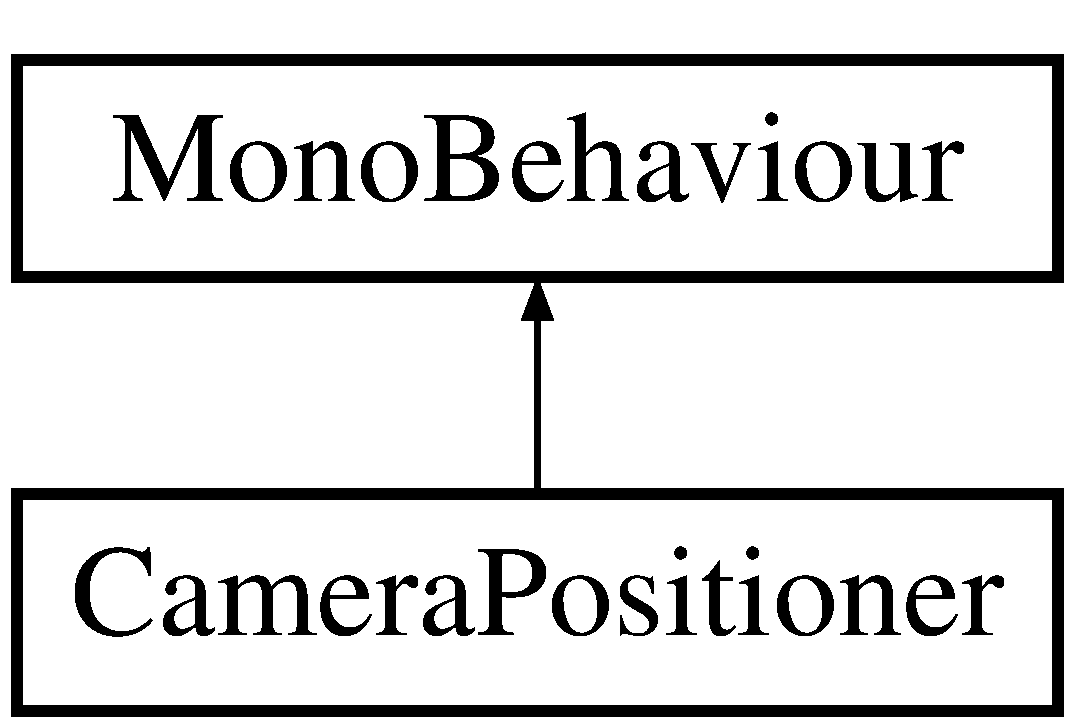
\includegraphics[height=2.000000cm]{class_camera_positioner}
\end{center}
\end{figure}
\subsection*{Public Attributes}
\begin{DoxyCompactItemize}
\item 
Game\+Object \mbox{\hyperlink{class_camera_positioner_a7ad34060c11c472c397d42cd92ff7d3f}{getter\+Obj}}
\end{DoxyCompactItemize}


\subsection{Member Data Documentation}
\mbox{\Hypertarget{class_camera_positioner_a7ad34060c11c472c397d42cd92ff7d3f}\label{class_camera_positioner_a7ad34060c11c472c397d42cd92ff7d3f}} 
\index{Camera\+Positioner@{Camera\+Positioner}!getter\+Obj@{getter\+Obj}}
\index{getter\+Obj@{getter\+Obj}!Camera\+Positioner@{Camera\+Positioner}}
\subsubsection{\texorpdfstring{getter\+Obj}{getterObj}}
{\footnotesize\ttfamily Game\+Object Camera\+Positioner.\+getter\+Obj}



The documentation for this class was generated from the following file\+:\begin{DoxyCompactItemize}
\item 
\mbox{\hyperlink{_camera_positioner_8cs}{Camera\+Positioner.\+cs}}\end{DoxyCompactItemize}

\hypertarget{class_comm_action}{}\section{Comm\+Action Class Reference}
\label{class_comm_action}\index{Comm\+Action@{Comm\+Action}}
Inheritance diagram for Comm\+Action\+:\begin{figure}[H]
\begin{center}
\leavevmode
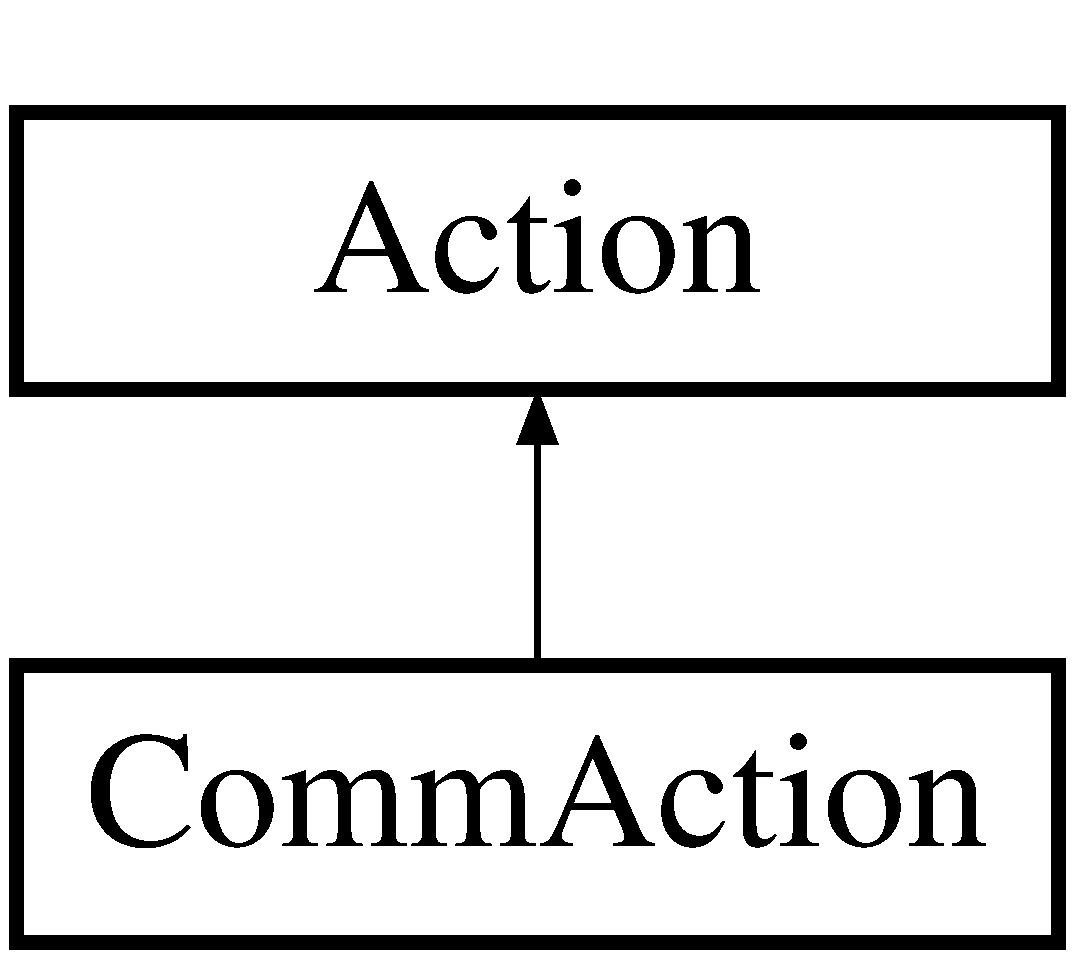
\includegraphics[height=2.000000cm]{class_comm_action}
\end{center}
\end{figure}
\subsection*{Public Member Functions}
\begin{DoxyCompactItemize}
\item 
override void \mbox{\hyperlink{class_comm_action_a4ea8e9bcc0a5060221efdc6afefa4355}{perform}} (\mbox{\hyperlink{class_creature}{Creature}} creature, \mbox{\hyperlink{class_ecosystem}{Ecosystem}} eco)
\begin{DoxyCompactList}\small\item\em Adds signal to creatures output comm signals. (to be iterated over and passed to neighbors). \end{DoxyCompactList}\item 
void \mbox{\hyperlink{class_comm_action_ab1c591777d0b6c2e567f69e7dd15e2c1}{assign\+Signal\+Props}} ()
\begin{DoxyCompactList}\small\item\em Assigns properties of signal \end{DoxyCompactList}\end{DoxyCompactItemize}
\subsection*{Additional Inherited Members}


\subsection{Member Function Documentation}
\mbox{\Hypertarget{class_comm_action_ab1c591777d0b6c2e567f69e7dd15e2c1}\label{class_comm_action_ab1c591777d0b6c2e567f69e7dd15e2c1}} 
\index{Comm\+Action@{Comm\+Action}!assign\+Signal\+Props@{assign\+Signal\+Props}}
\index{assign\+Signal\+Props@{assign\+Signal\+Props}!Comm\+Action@{Comm\+Action}}
\subsubsection{\texorpdfstring{assign\+Signal\+Props()}{assignSignalProps()}}
{\footnotesize\ttfamily void Comm\+Action.\+assign\+Signal\+Props (\begin{DoxyParamCaption}{ }\end{DoxyParamCaption})}



Assigns properties of signal 

\mbox{\Hypertarget{class_comm_action_a4ea8e9bcc0a5060221efdc6afefa4355}\label{class_comm_action_a4ea8e9bcc0a5060221efdc6afefa4355}} 
\index{Comm\+Action@{Comm\+Action}!perform@{perform}}
\index{perform@{perform}!Comm\+Action@{Comm\+Action}}
\subsubsection{\texorpdfstring{perform()}{perform()}}
{\footnotesize\ttfamily override void Comm\+Action.\+perform (\begin{DoxyParamCaption}\item[{\mbox{\hyperlink{class_creature}{Creature}}}]{creature,  }\item[{\mbox{\hyperlink{class_ecosystem}{Ecosystem}}}]{eco }\end{DoxyParamCaption})\hspace{0.3cm}{\ttfamily [virtual]}}



Adds signal to creatures output comm signals. (to be iterated over and passed to neighbors). 



Implements \mbox{\hyperlink{class_action_a2aedfc3be16448fbf224cb13607de3c0}{Action}}.



The documentation for this class was generated from the following file\+:\begin{DoxyCompactItemize}
\item 
\mbox{\hyperlink{_comm_action_8cs}{Comm\+Action.\+cs}}\end{DoxyCompactItemize}

\hypertarget{class_comm_action_editor}{}\section{Comm\+Action\+Editor Class Reference}
\label{class_comm_action_editor}\index{Comm\+Action\+Editor@{Comm\+Action\+Editor}}
Inheritance diagram for Comm\+Action\+Editor\+:\begin{figure}[H]
\begin{center}
\leavevmode
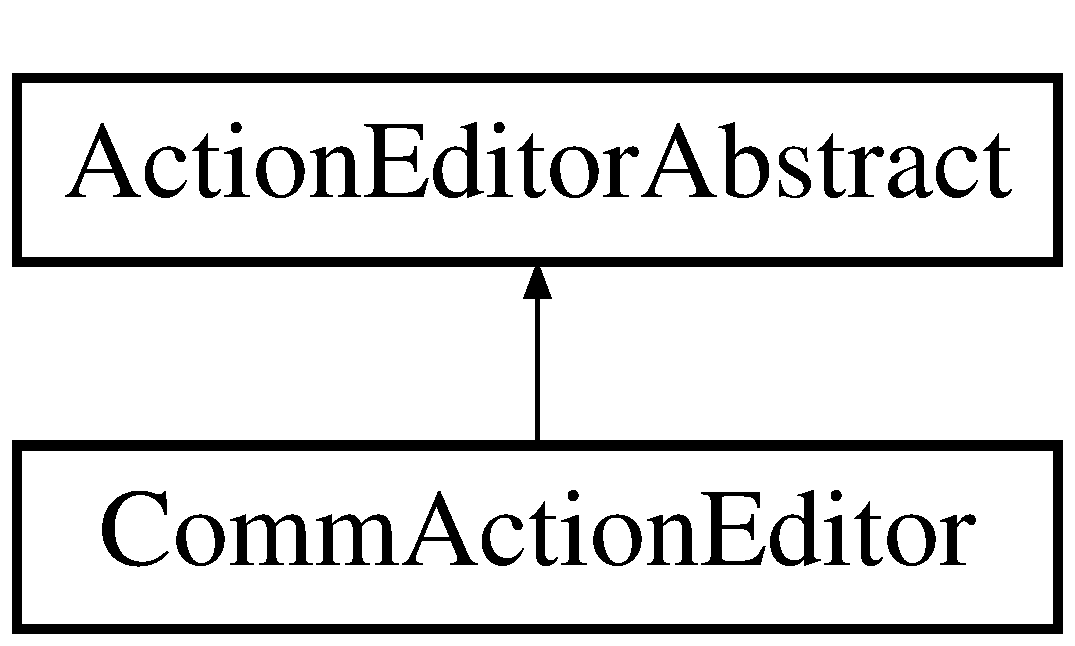
\includegraphics[height=2.000000cm]{class_comm_action_editor}
\end{center}
\end{figure}
\subsection*{Public Member Functions}
\begin{DoxyCompactItemize}
\item 
\mbox{\hyperlink{class_comm_action_editor_a8bb274b96f253d962d0fdf1dd9c3dc0c}{Comm\+Action\+Editor}} (\mbox{\hyperlink{class_comm_action}{Comm\+Action}} a)
\item 
void \mbox{\hyperlink{class_comm_action_editor_a2b01d693e77eb550d6366289bfc7a765}{set\+Comm\+Signal\+Properties}} ()
\end{DoxyCompactItemize}
\subsection*{Additional Inherited Members}


\subsection{Constructor \& Destructor Documentation}
\mbox{\Hypertarget{class_comm_action_editor_a8bb274b96f253d962d0fdf1dd9c3dc0c}\label{class_comm_action_editor_a8bb274b96f253d962d0fdf1dd9c3dc0c}} 
\index{Comm\+Action\+Editor@{Comm\+Action\+Editor}!Comm\+Action\+Editor@{Comm\+Action\+Editor}}
\index{Comm\+Action\+Editor@{Comm\+Action\+Editor}!Comm\+Action\+Editor@{Comm\+Action\+Editor}}
\subsubsection{\texorpdfstring{Comm\+Action\+Editor()}{CommActionEditor()}}
{\footnotesize\ttfamily Comm\+Action\+Editor.\+Comm\+Action\+Editor (\begin{DoxyParamCaption}\item[{\mbox{\hyperlink{class_comm_action}{Comm\+Action}}}]{a }\end{DoxyParamCaption})}



\subsection{Member Function Documentation}
\mbox{\Hypertarget{class_comm_action_editor_a2b01d693e77eb550d6366289bfc7a765}\label{class_comm_action_editor_a2b01d693e77eb550d6366289bfc7a765}} 
\index{Comm\+Action\+Editor@{Comm\+Action\+Editor}!set\+Comm\+Signal\+Properties@{set\+Comm\+Signal\+Properties}}
\index{set\+Comm\+Signal\+Properties@{set\+Comm\+Signal\+Properties}!Comm\+Action\+Editor@{Comm\+Action\+Editor}}
\subsubsection{\texorpdfstring{set\+Comm\+Signal\+Properties()}{setCommSignalProperties()}}
{\footnotesize\ttfamily void Comm\+Action\+Editor.\+set\+Comm\+Signal\+Properties (\begin{DoxyParamCaption}{ }\end{DoxyParamCaption})}



The documentation for this class was generated from the following file\+:\begin{DoxyCompactItemize}
\item 
\mbox{\hyperlink{_comm_action_editor_8cs}{Comm\+Action\+Editor.\+cs}}\end{DoxyCompactItemize}

\hypertarget{class_comm_input_node}{}\section{Comm\+Input\+Node Class Reference}
\label{class_comm_input_node}\index{Comm\+Input\+Node@{Comm\+Input\+Node}}
Inheritance diagram for Comm\+Input\+Node\+:\begin{figure}[H]
\begin{center}
\leavevmode
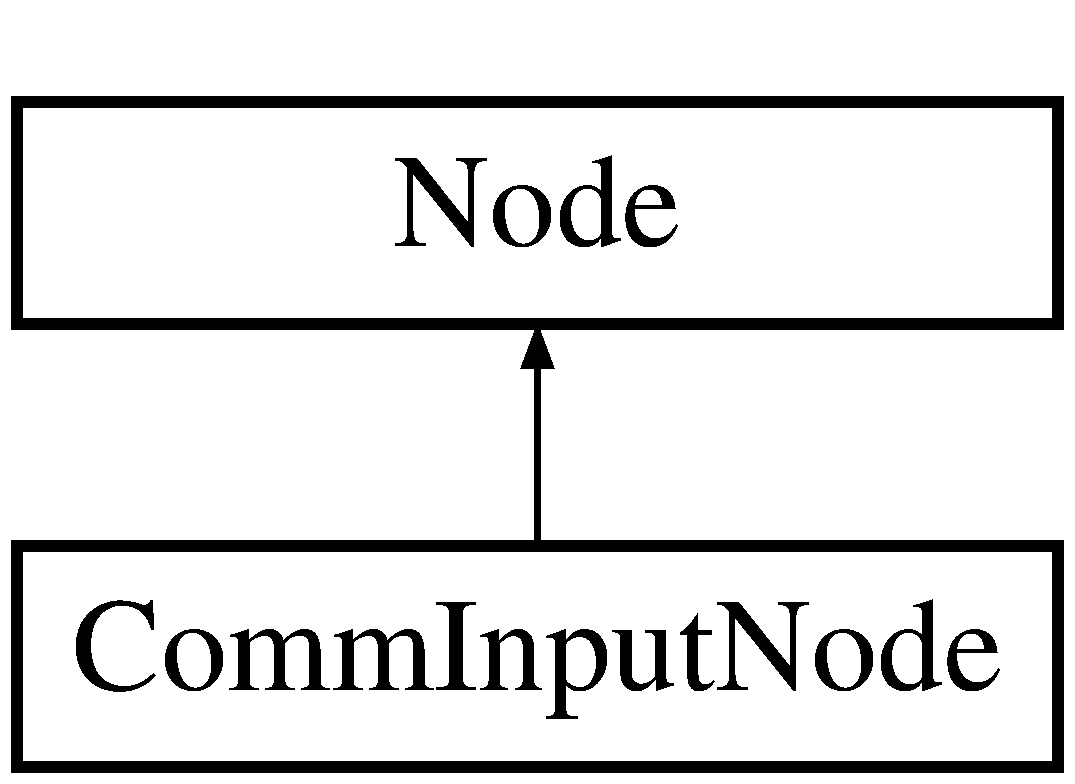
\includegraphics[height=2.000000cm]{class_comm_input_node}
\end{center}
\end{figure}
\subsection*{Public Member Functions}
\begin{DoxyCompactItemize}
\item 
override void \mbox{\hyperlink{class_comm_input_node_a22f5ea13329e77f47db18d28336cc52e}{update\+Value}} ()
\begin{DoxyCompactList}\small\item\em Will check if a creature is at this neighbor, and get it\textquotesingle{}s comm output, or otherwise sets value to 0. \end{DoxyCompactList}\end{DoxyCompactItemize}
\subsection*{Public Attributes}
\begin{DoxyCompactItemize}
\item 
\mbox{\hyperlink{class_creature}{Creature}} \mbox{\hyperlink{class_comm_input_node_ac72fbeea2e0341d3caaddd99f9a71cb6}{creature}}
\begin{DoxyCompactList}\small\item\em Stores reference to creature for getting access to neighbors \end{DoxyCompactList}\item 
string \mbox{\hyperlink{class_comm_input_node_a1a81a36b88a72dacb21af46740a3bfda}{comm\+Property}}
\begin{DoxyCompactList}\small\item\em stores which property to access in \mbox{\hyperlink{class_comm_signal}{Comm\+Signal}} \end{DoxyCompactList}\item 
int \mbox{\hyperlink{class_comm_input_node_a37287af65740dffcdb3c36630264ded8}{bit\+Index}}
\begin{DoxyCompactList}\small\item\em Stores index of specific bit to convert to 0 or 1 from a particular property of the \mbox{\hyperlink{class_comm_signal}{Comm\+Signal}}. \end{DoxyCompactList}\end{DoxyCompactItemize}


\subsection{Member Function Documentation}
\mbox{\Hypertarget{class_comm_input_node_a22f5ea13329e77f47db18d28336cc52e}\label{class_comm_input_node_a22f5ea13329e77f47db18d28336cc52e}} 
\index{Comm\+Input\+Node@{Comm\+Input\+Node}!update\+Value@{update\+Value}}
\index{update\+Value@{update\+Value}!Comm\+Input\+Node@{Comm\+Input\+Node}}
\subsubsection{\texorpdfstring{update\+Value()}{updateValue()}}
{\footnotesize\ttfamily override void Comm\+Input\+Node.\+update\+Value (\begin{DoxyParamCaption}{ }\end{DoxyParamCaption})\hspace{0.3cm}{\ttfamily [virtual]}}



Will check if a creature is at this neighbor, and get it\textquotesingle{}s comm output, or otherwise sets value to 0. 



Implements \mbox{\hyperlink{class_node_a85ebd0e36c25430570b94f923afd2a62}{Node}}.



\subsection{Member Data Documentation}
\mbox{\Hypertarget{class_comm_input_node_a37287af65740dffcdb3c36630264ded8}\label{class_comm_input_node_a37287af65740dffcdb3c36630264ded8}} 
\index{Comm\+Input\+Node@{Comm\+Input\+Node}!bit\+Index@{bit\+Index}}
\index{bit\+Index@{bit\+Index}!Comm\+Input\+Node@{Comm\+Input\+Node}}
\subsubsection{\texorpdfstring{bit\+Index}{bitIndex}}
{\footnotesize\ttfamily int Comm\+Input\+Node.\+bit\+Index}



Stores index of specific bit to convert to 0 or 1 from a particular property of the \mbox{\hyperlink{class_comm_signal}{Comm\+Signal}}. 

\mbox{\Hypertarget{class_comm_input_node_a1a81a36b88a72dacb21af46740a3bfda}\label{class_comm_input_node_a1a81a36b88a72dacb21af46740a3bfda}} 
\index{Comm\+Input\+Node@{Comm\+Input\+Node}!comm\+Property@{comm\+Property}}
\index{comm\+Property@{comm\+Property}!Comm\+Input\+Node@{Comm\+Input\+Node}}
\subsubsection{\texorpdfstring{comm\+Property}{commProperty}}
{\footnotesize\ttfamily string Comm\+Input\+Node.\+comm\+Property}



stores which property to access in \mbox{\hyperlink{class_comm_signal}{Comm\+Signal}} 

\mbox{\Hypertarget{class_comm_input_node_ac72fbeea2e0341d3caaddd99f9a71cb6}\label{class_comm_input_node_ac72fbeea2e0341d3caaddd99f9a71cb6}} 
\index{Comm\+Input\+Node@{Comm\+Input\+Node}!creature@{creature}}
\index{creature@{creature}!Comm\+Input\+Node@{Comm\+Input\+Node}}
\subsubsection{\texorpdfstring{creature}{creature}}
{\footnotesize\ttfamily \mbox{\hyperlink{class_creature}{Creature}} Comm\+Input\+Node.\+creature}



Stores reference to creature for getting access to neighbors 



The documentation for this class was generated from the following file\+:\begin{DoxyCompactItemize}
\item 
\mbox{\hyperlink{_comm_input_node_8cs}{Comm\+Input\+Node.\+cs}}\end{DoxyCompactItemize}

\hypertarget{class_comm_network}{}\section{Comm\+Network Class Reference}
\label{class_comm_network}\index{Comm\+Network@{Comm\+Network}}


A network that converts incomming comm signals into action recommendations. A seperate comm network is needed for every neightbor that sends a comm signal.  


Inheritance diagram for Comm\+Network\+:\begin{figure}[H]
\begin{center}
\leavevmode
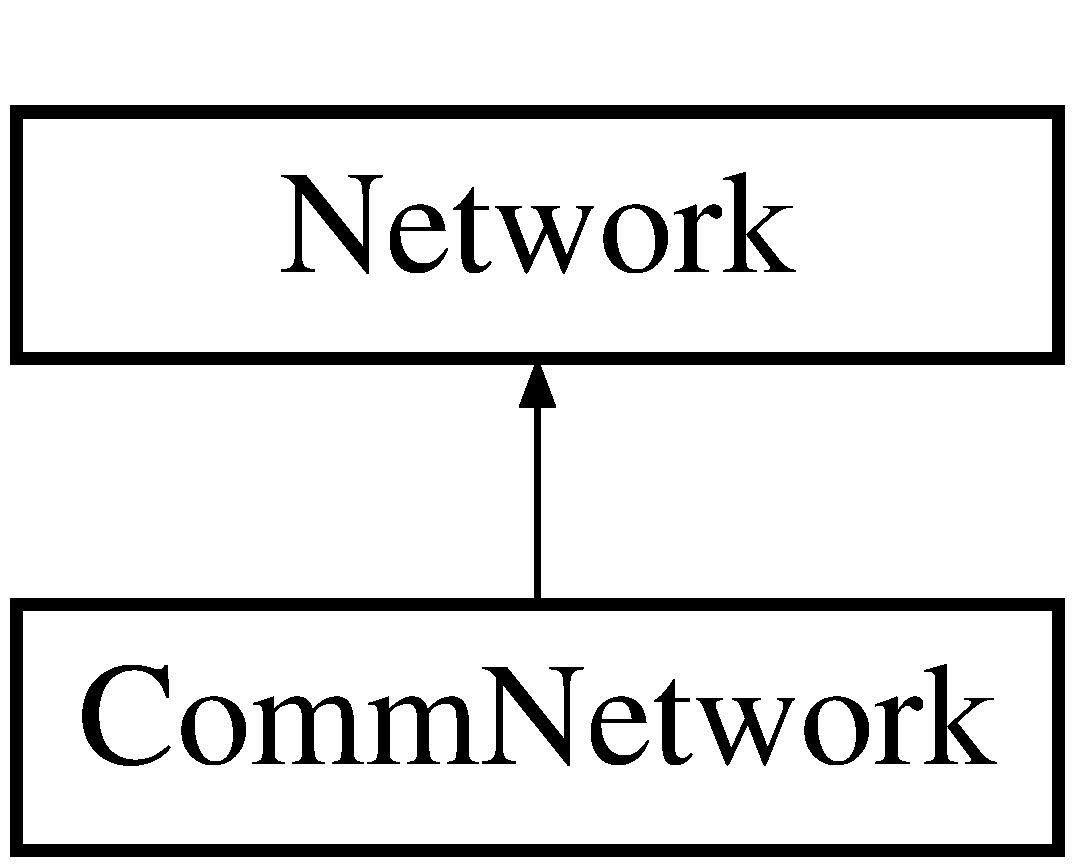
\includegraphics[height=2.000000cm]{class_comm_network}
\end{center}
\end{figure}
\subsection*{Public Member Functions}
\begin{DoxyCompactItemize}
\item 
\mbox{\hyperlink{class_comm_network}{Comm\+Network}} \mbox{\hyperlink{class_comm_network_a22078a6183c8ca5be7b40964d57d1258}{get\+Shallow\+Copy}} ()
\end{DoxyCompactItemize}
\subsection*{Additional Inherited Members}


\subsection{Detailed Description}
A network that converts incomming comm signals into action recommendations. A seperate comm network is needed for every neightbor that sends a comm signal. 



\subsection{Member Function Documentation}
\mbox{\Hypertarget{class_comm_network_a22078a6183c8ca5be7b40964d57d1258}\label{class_comm_network_a22078a6183c8ca5be7b40964d57d1258}} 
\index{Comm\+Network@{Comm\+Network}!get\+Shallow\+Copy@{get\+Shallow\+Copy}}
\index{get\+Shallow\+Copy@{get\+Shallow\+Copy}!Comm\+Network@{Comm\+Network}}
\subsubsection{\texorpdfstring{get\+Shallow\+Copy()}{getShallowCopy()}}
{\footnotesize\ttfamily \mbox{\hyperlink{class_comm_network}{Comm\+Network}} Comm\+Network.\+get\+Shallow\+Copy (\begin{DoxyParamCaption}{ }\end{DoxyParamCaption})}



The documentation for this class was generated from the following file\+:\begin{DoxyCompactItemize}
\item 
\mbox{\hyperlink{_comm_network_8cs}{Comm\+Network.\+cs}}\end{DoxyCompactItemize}

\hypertarget{class_comm_node_editor}{}\section{Comm\+Node\+Editor Class Reference}
\label{class_comm_node_editor}\index{Comm\+Node\+Editor@{Comm\+Node\+Editor}}


A\+PI for Comm Nodes  


Inheritance diagram for Comm\+Node\+Editor\+:\begin{figure}[H]
\begin{center}
\leavevmode
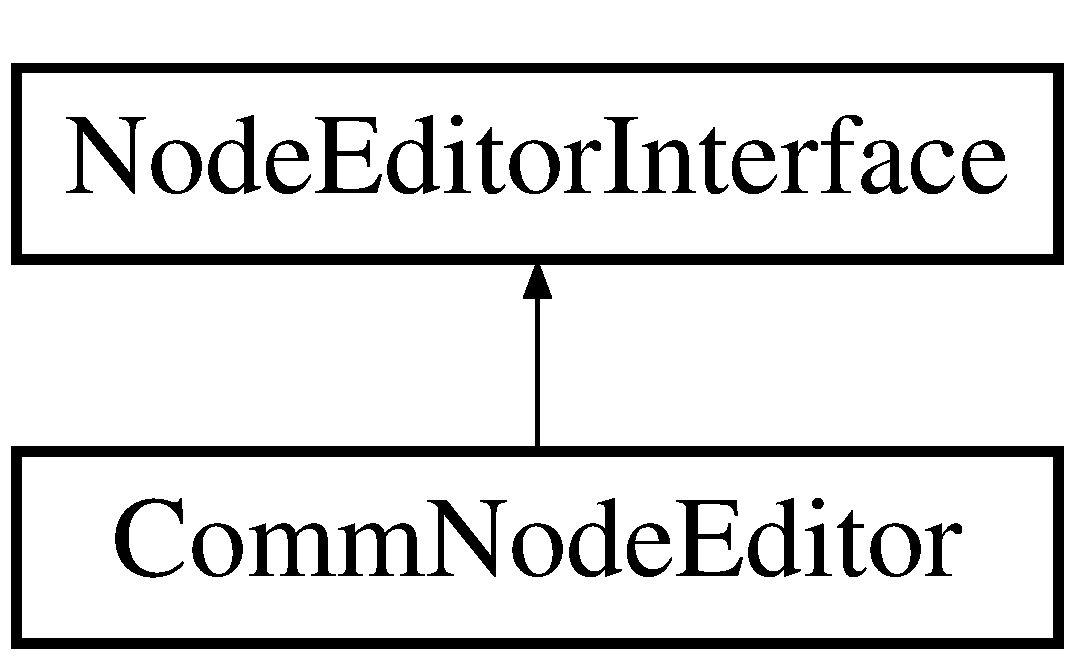
\includegraphics[height=2.000000cm]{class_comm_node_editor}
\end{center}
\end{figure}
\subsection*{Public Member Functions}
\begin{DoxyCompactItemize}
\item 
\mbox{\hyperlink{class_comm_node_editor_aca81fedc55a41cfbd42f8e00f05a7f32}{Comm\+Node\+Editor}} (\mbox{\hyperlink{class_comm_input_node}{Comm\+Input\+Node}} \+\_\+comm\+Node, int \+\_\+node\+Layer)
\item 
\mbox{\hyperlink{class_node}{Node}} \mbox{\hyperlink{class_comm_node_editor_ad578649fe7c3775e0b91c1acdb5e738a}{get\+Node}} ()
\end{DoxyCompactItemize}
\subsection*{Public Attributes}
\begin{DoxyCompactItemize}
\item 
\mbox{\hyperlink{class_comm_input_node}{Comm\+Input\+Node}} \mbox{\hyperlink{class_comm_node_editor_a36b489d896bf2c7cb2128f3b139008d2}{comm\+Node}}
\item 
int \mbox{\hyperlink{class_comm_node_editor_a23b382bbd6d5fc07966f04e09bd75093}{node\+Layer}}
\end{DoxyCompactItemize}


\subsection{Detailed Description}
A\+PI for Comm Nodes 



\subsection{Constructor \& Destructor Documentation}
\mbox{\Hypertarget{class_comm_node_editor_aca81fedc55a41cfbd42f8e00f05a7f32}\label{class_comm_node_editor_aca81fedc55a41cfbd42f8e00f05a7f32}} 
\index{Comm\+Node\+Editor@{Comm\+Node\+Editor}!Comm\+Node\+Editor@{Comm\+Node\+Editor}}
\index{Comm\+Node\+Editor@{Comm\+Node\+Editor}!Comm\+Node\+Editor@{Comm\+Node\+Editor}}
\subsubsection{\texorpdfstring{Comm\+Node\+Editor()}{CommNodeEditor()}}
{\footnotesize\ttfamily Comm\+Node\+Editor.\+Comm\+Node\+Editor (\begin{DoxyParamCaption}\item[{\mbox{\hyperlink{class_comm_input_node}{Comm\+Input\+Node}}}]{\+\_\+comm\+Node,  }\item[{int}]{\+\_\+node\+Layer }\end{DoxyParamCaption})}



\subsection{Member Function Documentation}
\mbox{\Hypertarget{class_comm_node_editor_ad578649fe7c3775e0b91c1acdb5e738a}\label{class_comm_node_editor_ad578649fe7c3775e0b91c1acdb5e738a}} 
\index{Comm\+Node\+Editor@{Comm\+Node\+Editor}!get\+Node@{get\+Node}}
\index{get\+Node@{get\+Node}!Comm\+Node\+Editor@{Comm\+Node\+Editor}}
\subsubsection{\texorpdfstring{get\+Node()}{getNode()}}
{\footnotesize\ttfamily \mbox{\hyperlink{class_node}{Node}} Comm\+Node\+Editor.\+get\+Node (\begin{DoxyParamCaption}{ }\end{DoxyParamCaption})}



Implements \mbox{\hyperlink{interface_node_editor_interface_a56e2abaedf17d7fbf2be90d521ec9363}{Node\+Editor\+Interface}}.



\subsection{Member Data Documentation}
\mbox{\Hypertarget{class_comm_node_editor_a36b489d896bf2c7cb2128f3b139008d2}\label{class_comm_node_editor_a36b489d896bf2c7cb2128f3b139008d2}} 
\index{Comm\+Node\+Editor@{Comm\+Node\+Editor}!comm\+Node@{comm\+Node}}
\index{comm\+Node@{comm\+Node}!Comm\+Node\+Editor@{Comm\+Node\+Editor}}
\subsubsection{\texorpdfstring{comm\+Node}{commNode}}
{\footnotesize\ttfamily \mbox{\hyperlink{class_comm_input_node}{Comm\+Input\+Node}} Comm\+Node\+Editor.\+comm\+Node}

\mbox{\Hypertarget{class_comm_node_editor_a23b382bbd6d5fc07966f04e09bd75093}\label{class_comm_node_editor_a23b382bbd6d5fc07966f04e09bd75093}} 
\index{Comm\+Node\+Editor@{Comm\+Node\+Editor}!node\+Layer@{node\+Layer}}
\index{node\+Layer@{node\+Layer}!Comm\+Node\+Editor@{Comm\+Node\+Editor}}
\subsubsection{\texorpdfstring{node\+Layer}{nodeLayer}}
{\footnotesize\ttfamily int Comm\+Node\+Editor.\+node\+Layer}



The documentation for this class was generated from the following file\+:\begin{DoxyCompactItemize}
\item 
\mbox{\hyperlink{_comm_node_editor_8cs}{Comm\+Node\+Editor.\+cs}}\end{DoxyCompactItemize}

\hypertarget{class_comm_signal}{}\section{Comm\+Signal Class Reference}
\label{class_comm_signal}\index{Comm\+Signal@{Comm\+Signal}}


The comm network must individually process each comm signal stored in the creatures comm\+List, and save the outputs as action recommendations.  


\subsection*{Public Attributes}
\begin{DoxyCompactItemize}
\item 
Dictionary$<$ string, bool\mbox{[}$\,$\mbox{]}$>$ \mbox{\hyperlink{class_comm_signal_a417bfc34bf6a9cc2779f2c02fe23ee4b}{comm\+Properties}}
\begin{DoxyCompactList}\small\item\em Stores message, position, and phenotype. \end{DoxyCompactList}\end{DoxyCompactItemize}


\subsection{Detailed Description}
The comm network must individually process each comm signal stored in the creatures comm\+List, and save the outputs as action recommendations. 



\subsection{Member Data Documentation}
\mbox{\Hypertarget{class_comm_signal_a417bfc34bf6a9cc2779f2c02fe23ee4b}\label{class_comm_signal_a417bfc34bf6a9cc2779f2c02fe23ee4b}} 
\index{Comm\+Signal@{Comm\+Signal}!comm\+Properties@{comm\+Properties}}
\index{comm\+Properties@{comm\+Properties}!Comm\+Signal@{Comm\+Signal}}
\subsubsection{\texorpdfstring{comm\+Properties}{commProperties}}
{\footnotesize\ttfamily Dictionary$<$string, bool\mbox{[}$\,$\mbox{]}$>$ Comm\+Signal.\+comm\+Properties}



Stores message, position, and phenotype. 



The documentation for this class was generated from the following file\+:\begin{DoxyCompactItemize}
\item 
\mbox{\hyperlink{_comm_signal_8cs}{Comm\+Signal.\+cs}}\end{DoxyCompactItemize}

\hypertarget{class_consume_from_land}{}\section{Consume\+From\+Land Class Reference}
\label{class_consume_from_land}\index{Consume\+From\+Land@{Consume\+From\+Land}}
Inheritance diagram for Consume\+From\+Land\+:\begin{figure}[H]
\begin{center}
\leavevmode
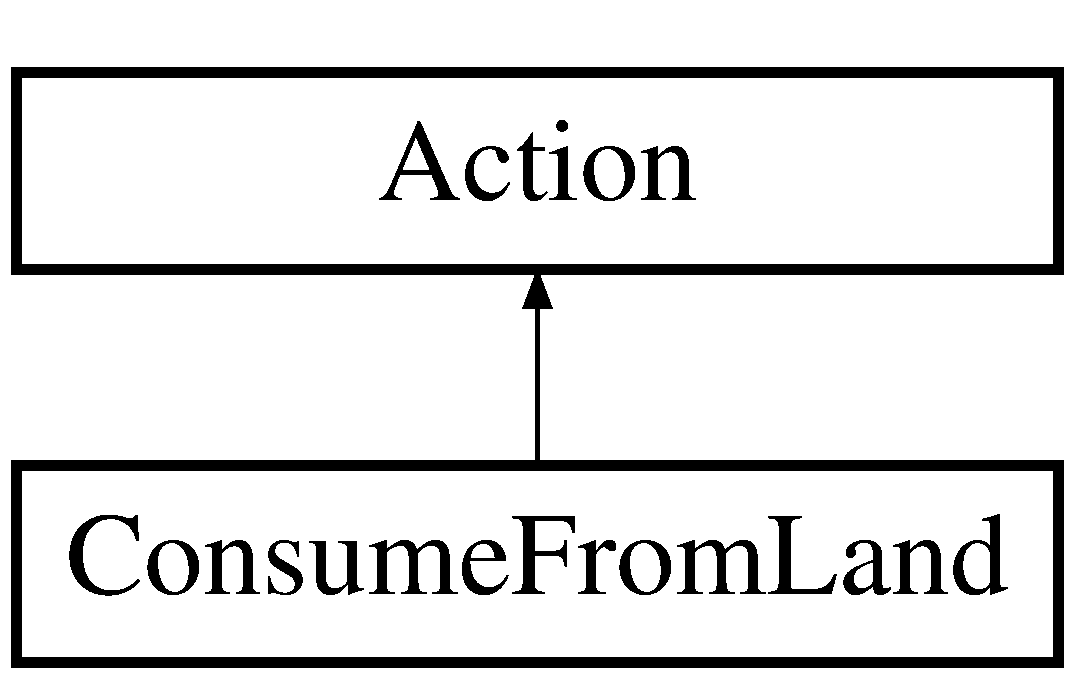
\includegraphics[height=2.000000cm]{class_consume_from_land}
\end{center}
\end{figure}
\subsection*{Public Member Functions}
\begin{DoxyCompactItemize}
\item 
\mbox{\hyperlink{class_consume_from_land_a5496a937e22a90235f5df516af9cd133}{Consume\+From\+Land}} ()
\item 
\mbox{\hyperlink{class_consume_from_land_a7168ad8a66c20529d60930de930bfafe}{Consume\+From\+Land}} (int \mbox{\hyperlink{class_consume_from_land_a645ca79e901a05c787df9e35d3a0318b}{neighbor\+Index}}, string \mbox{\hyperlink{class_consume_from_land_a4ef240b29ec3b427fca36c8de1fed24b}{resource\+To\+Consume}})
\item 
override void \mbox{\hyperlink{class_consume_from_land_a05e266fe8dd4d68b7bec63f53a7f513b}{perform}} (\mbox{\hyperlink{class_creature}{Creature}} creature, \mbox{\hyperlink{class_ecosystem}{Ecosystem}} eco)
\begin{DoxyCompactList}\small\item\em Accesses land via neighbor\+Index, and attemps to consume resource. \end{DoxyCompactList}\item 
System.\+Object \mbox{\hyperlink{class_consume_from_land_a352f47add666c68f6ab9c901280b9de1}{clone}} ()
\end{DoxyCompactItemize}
\subsection*{Public Attributes}
\begin{DoxyCompactItemize}
\item 
int \mbox{\hyperlink{class_consume_from_land_a645ca79e901a05c787df9e35d3a0318b}{neighbor\+Index}}
\begin{DoxyCompactList}\small\item\em Index of neighboring land to access. \end{DoxyCompactList}\item 
string \mbox{\hyperlink{class_consume_from_land_a4ef240b29ec3b427fca36c8de1fed24b}{resource\+To\+Consume}}
\begin{DoxyCompactList}\small\item\em Name of resource to consume. \end{DoxyCompactList}\end{DoxyCompactItemize}


\subsection{Constructor \& Destructor Documentation}
\mbox{\Hypertarget{class_consume_from_land_a5496a937e22a90235f5df516af9cd133}\label{class_consume_from_land_a5496a937e22a90235f5df516af9cd133}} 
\index{Consume\+From\+Land@{Consume\+From\+Land}!Consume\+From\+Land@{Consume\+From\+Land}}
\index{Consume\+From\+Land@{Consume\+From\+Land}!Consume\+From\+Land@{Consume\+From\+Land}}
\subsubsection{\texorpdfstring{Consume\+From\+Land()}{ConsumeFromLand()}\hspace{0.1cm}{\footnotesize\ttfamily [1/2]}}
{\footnotesize\ttfamily Consume\+From\+Land.\+Consume\+From\+Land (\begin{DoxyParamCaption}{ }\end{DoxyParamCaption})}

\mbox{\Hypertarget{class_consume_from_land_a7168ad8a66c20529d60930de930bfafe}\label{class_consume_from_land_a7168ad8a66c20529d60930de930bfafe}} 
\index{Consume\+From\+Land@{Consume\+From\+Land}!Consume\+From\+Land@{Consume\+From\+Land}}
\index{Consume\+From\+Land@{Consume\+From\+Land}!Consume\+From\+Land@{Consume\+From\+Land}}
\subsubsection{\texorpdfstring{Consume\+From\+Land()}{ConsumeFromLand()}\hspace{0.1cm}{\footnotesize\ttfamily [2/2]}}
{\footnotesize\ttfamily Consume\+From\+Land.\+Consume\+From\+Land (\begin{DoxyParamCaption}\item[{int}]{neighbor\+Index,  }\item[{string}]{resource\+To\+Consume }\end{DoxyParamCaption})}



\subsection{Member Function Documentation}
\mbox{\Hypertarget{class_consume_from_land_a352f47add666c68f6ab9c901280b9de1}\label{class_consume_from_land_a352f47add666c68f6ab9c901280b9de1}} 
\index{Consume\+From\+Land@{Consume\+From\+Land}!clone@{clone}}
\index{clone@{clone}!Consume\+From\+Land@{Consume\+From\+Land}}
\subsubsection{\texorpdfstring{clone()}{clone()}}
{\footnotesize\ttfamily System.\+Object Consume\+From\+Land.\+clone (\begin{DoxyParamCaption}{ }\end{DoxyParamCaption})}

\mbox{\Hypertarget{class_consume_from_land_a05e266fe8dd4d68b7bec63f53a7f513b}\label{class_consume_from_land_a05e266fe8dd4d68b7bec63f53a7f513b}} 
\index{Consume\+From\+Land@{Consume\+From\+Land}!perform@{perform}}
\index{perform@{perform}!Consume\+From\+Land@{Consume\+From\+Land}}
\subsubsection{\texorpdfstring{perform()}{perform()}}
{\footnotesize\ttfamily override void Consume\+From\+Land.\+perform (\begin{DoxyParamCaption}\item[{\mbox{\hyperlink{class_creature}{Creature}}}]{creature,  }\item[{\mbox{\hyperlink{class_ecosystem}{Ecosystem}}}]{eco }\end{DoxyParamCaption})\hspace{0.3cm}{\ttfamily [virtual]}}



Accesses land via neighbor\+Index, and attemps to consume resource. 



Implements \mbox{\hyperlink{class_action_a2aedfc3be16448fbf224cb13607de3c0}{Action}}.



\subsection{Member Data Documentation}
\mbox{\Hypertarget{class_consume_from_land_a645ca79e901a05c787df9e35d3a0318b}\label{class_consume_from_land_a645ca79e901a05c787df9e35d3a0318b}} 
\index{Consume\+From\+Land@{Consume\+From\+Land}!neighbor\+Index@{neighbor\+Index}}
\index{neighbor\+Index@{neighbor\+Index}!Consume\+From\+Land@{Consume\+From\+Land}}
\subsubsection{\texorpdfstring{neighbor\+Index}{neighborIndex}}
{\footnotesize\ttfamily int Consume\+From\+Land.\+neighbor\+Index}



Index of neighboring land to access. 

\mbox{\Hypertarget{class_consume_from_land_a4ef240b29ec3b427fca36c8de1fed24b}\label{class_consume_from_land_a4ef240b29ec3b427fca36c8de1fed24b}} 
\index{Consume\+From\+Land@{Consume\+From\+Land}!resource\+To\+Consume@{resource\+To\+Consume}}
\index{resource\+To\+Consume@{resource\+To\+Consume}!Consume\+From\+Land@{Consume\+From\+Land}}
\subsubsection{\texorpdfstring{resource\+To\+Consume}{resourceToConsume}}
{\footnotesize\ttfamily string Consume\+From\+Land.\+resource\+To\+Consume}



Name of resource to consume. 



The documentation for this class was generated from the following file\+:\begin{DoxyCompactItemize}
\item 
\mbox{\hyperlink{_consume_from_land_8cs}{Consume\+From\+Land.\+cs}}\end{DoxyCompactItemize}

\hypertarget{class_consume_from_land_editor}{}\section{Consume\+From\+Land\+Editor Class Reference}
\label{class_consume_from_land_editor}\index{Consume\+From\+Land\+Editor@{Consume\+From\+Land\+Editor}}
Inheritance diagram for Consume\+From\+Land\+Editor\+:\begin{figure}[H]
\begin{center}
\leavevmode
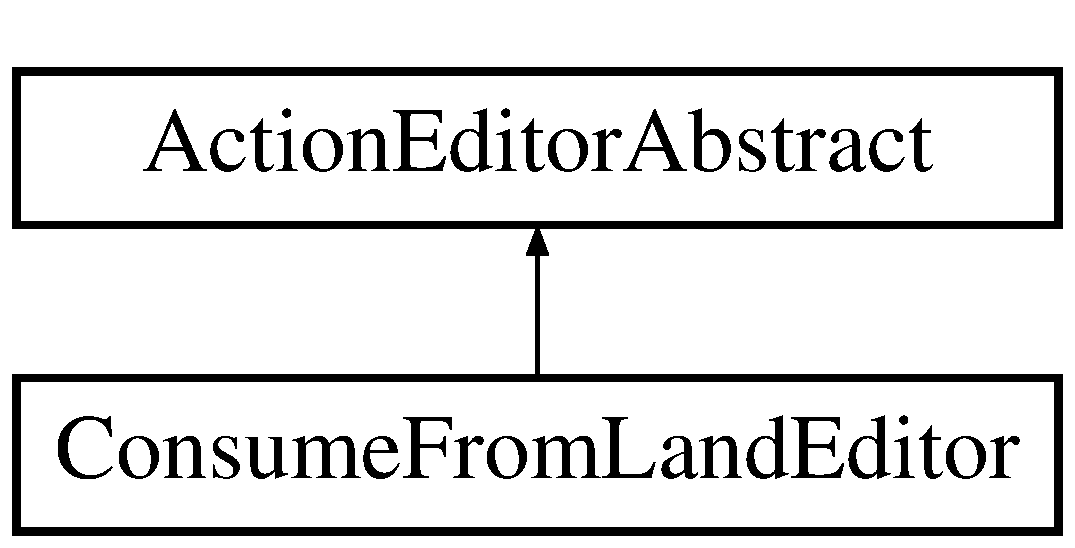
\includegraphics[height=2.000000cm]{class_consume_from_land_editor}
\end{center}
\end{figure}
\subsection*{Public Member Functions}
\begin{DoxyCompactItemize}
\item 
\mbox{\hyperlink{class_consume_from_land_editor_a7f47060c9426914caeb00cc78db6cf74}{Consume\+From\+Land\+Editor}} (\mbox{\hyperlink{class_consume_from_land}{Consume\+From\+Land}} in\+Action)
\item 
void \mbox{\hyperlink{class_consume_from_land_editor_a8c3ecdabdf02fc94888ed16665f0850c}{set\+Neighbor\+Index}} (int index)
\item 
void \mbox{\hyperlink{class_consume_from_land_editor_a656aefcc2ccf0562992d48a59c8148de}{set\+Resource\+To\+Consume}} (string res)
\end{DoxyCompactItemize}
\subsection*{Additional Inherited Members}


\subsection{Constructor \& Destructor Documentation}
\mbox{\Hypertarget{class_consume_from_land_editor_a7f47060c9426914caeb00cc78db6cf74}\label{class_consume_from_land_editor_a7f47060c9426914caeb00cc78db6cf74}} 
\index{Consume\+From\+Land\+Editor@{Consume\+From\+Land\+Editor}!Consume\+From\+Land\+Editor@{Consume\+From\+Land\+Editor}}
\index{Consume\+From\+Land\+Editor@{Consume\+From\+Land\+Editor}!Consume\+From\+Land\+Editor@{Consume\+From\+Land\+Editor}}
\subsubsection{\texorpdfstring{Consume\+From\+Land\+Editor()}{ConsumeFromLandEditor()}}
{\footnotesize\ttfamily Consume\+From\+Land\+Editor.\+Consume\+From\+Land\+Editor (\begin{DoxyParamCaption}\item[{\mbox{\hyperlink{class_consume_from_land}{Consume\+From\+Land}}}]{in\+Action }\end{DoxyParamCaption})}



\subsection{Member Function Documentation}
\mbox{\Hypertarget{class_consume_from_land_editor_a8c3ecdabdf02fc94888ed16665f0850c}\label{class_consume_from_land_editor_a8c3ecdabdf02fc94888ed16665f0850c}} 
\index{Consume\+From\+Land\+Editor@{Consume\+From\+Land\+Editor}!set\+Neighbor\+Index@{set\+Neighbor\+Index}}
\index{set\+Neighbor\+Index@{set\+Neighbor\+Index}!Consume\+From\+Land\+Editor@{Consume\+From\+Land\+Editor}}
\subsubsection{\texorpdfstring{set\+Neighbor\+Index()}{setNeighborIndex()}}
{\footnotesize\ttfamily void Consume\+From\+Land\+Editor.\+set\+Neighbor\+Index (\begin{DoxyParamCaption}\item[{int}]{index }\end{DoxyParamCaption})}

\mbox{\Hypertarget{class_consume_from_land_editor_a656aefcc2ccf0562992d48a59c8148de}\label{class_consume_from_land_editor_a656aefcc2ccf0562992d48a59c8148de}} 
\index{Consume\+From\+Land\+Editor@{Consume\+From\+Land\+Editor}!set\+Resource\+To\+Consume@{set\+Resource\+To\+Consume}}
\index{set\+Resource\+To\+Consume@{set\+Resource\+To\+Consume}!Consume\+From\+Land\+Editor@{Consume\+From\+Land\+Editor}}
\subsubsection{\texorpdfstring{set\+Resource\+To\+Consume()}{setResourceToConsume()}}
{\footnotesize\ttfamily void Consume\+From\+Land\+Editor.\+set\+Resource\+To\+Consume (\begin{DoxyParamCaption}\item[{string}]{res }\end{DoxyParamCaption})}



The documentation for this class was generated from the following file\+:\begin{DoxyCompactItemize}
\item 
\mbox{\hyperlink{_consume_from_land_editor_8cs}{Consume\+From\+Land\+Editor.\+cs}}\end{DoxyCompactItemize}

\hypertarget{class_copier}{}\section{Copier Class Reference}
\label{class_copier}\index{Copier@{Copier}}
\subsection*{Static Public Member Functions}
\begin{DoxyCompactItemize}
\item 
static \mbox{\hyperlink{class_ecosystem}{Ecosystem}} \mbox{\hyperlink{class_copier_a19904060ea391728436f2f36ddf36a73}{get\+Ecosystem\+Copy}} (\mbox{\hyperlink{class_ecosystem}{Ecosystem}} eco)
\item 
static float \mbox{\hyperlink{class_copier_a187d00289a5f7c8d3b2d20a3468e9416}{norm\+Rand}} (float sd)
\item 
static \mbox{\hyperlink{class_land}{Land}} \mbox{\hyperlink{class_copier_ac38173e26db80dad92a6ca9cd083f058}{Get\+Land\+Copy}} (\mbox{\hyperlink{class_land}{Land}} land)
\item 
static \mbox{\hyperlink{class_creature}{Creature}} \mbox{\hyperlink{class_copier_a399f96d475da045dd0e9434c9054f161}{get\+Creature\+Child}} (\mbox{\hyperlink{class_creature}{Creature}} c)
\item 
static \mbox{\hyperlink{class_creature}{Creature}} \mbox{\hyperlink{class_copier_a468c753ccc3b2192bb49b8be03edf18c}{get\+Creature\+Copy}} (\mbox{\hyperlink{class_creature}{Creature}} c)
\item 
static void \mbox{\hyperlink{class_copier_a4013b1f8da509a6471f0feed3ec94ae3}{copy\+Comm\+List}} (List$<$ \mbox{\hyperlink{class_comm_signal}{Comm\+Signal}} $>$ orig\+List, List$<$ \mbox{\hyperlink{class_comm_signal}{Comm\+Signal}} $>$ copy\+List)
\item 
static void \mbox{\hyperlink{class_copier_a4c529b374830077f75db4520bb55e225}{copy\+Creature\+Networks}} (List$<$ Dictionary$<$ string, \mbox{\hyperlink{class_network}{Network}} $>$$>$ orig\+Networks, List$<$ Dictionary$<$ string, \mbox{\hyperlink{class_network}{Network}} $>$$>$ copy\+Networks, \mbox{\hyperlink{class_creature}{Creature}} creature\+Copy)
\item 
static \mbox{\hyperlink{class_ability}{Ability}} \mbox{\hyperlink{class_copier_a0912151eec03dadf8d375bde174522aa}{get\+New\+Ability}} (\mbox{\hyperlink{class_ability}{Ability}} old\+Ability)
\item 
static \mbox{\hyperlink{class_action}{Action}} \mbox{\hyperlink{class_copier_a12cae9390220b2dcee8472e3ab5ec38f}{get\+New\+Action}} (\mbox{\hyperlink{class_action}{Action}} old\+Action)
\item 
static \mbox{\hyperlink{class_node}{Node}} \mbox{\hyperlink{class_copier_a2bc3b60cb77fb710cf7e4802ceb16d03}{get\+New\+Node}} (\mbox{\hyperlink{class_node}{Node}} old\+Node, \mbox{\hyperlink{class_creature}{Creature}} creature\+Copy, \mbox{\hyperlink{class_network}{Network}} parent\+Net)
\end{DoxyCompactItemize}
\subsection*{Static Public Attributes}
\begin{DoxyCompactItemize}
\item 
static System.\+Random \mbox{\hyperlink{class_copier_ac2bbed854907158508f714b65783418e}{rand}} = new System.\+Random()
\item 
static System.\+Random \mbox{\hyperlink{class_copier_a74089df571f0e9ffadd5879bf0199dac}{seed\+Gen}} = new System.\+Random()
\item 
static int \mbox{\hyperlink{class_copier_a5f70131c00bf001cc92dd4cee4a80540}{seed}} = 0
\item 
static int \mbox{\hyperlink{class_copier_ab7101a9420cdd74139f3c83d9ec8ed25}{creature\+Num}} = 0
\end{DoxyCompactItemize}


\subsection{Member Function Documentation}
\mbox{\Hypertarget{class_copier_a4013b1f8da509a6471f0feed3ec94ae3}\label{class_copier_a4013b1f8da509a6471f0feed3ec94ae3}} 
\index{Copier@{Copier}!copy\+Comm\+List@{copy\+Comm\+List}}
\index{copy\+Comm\+List@{copy\+Comm\+List}!Copier@{Copier}}
\subsubsection{\texorpdfstring{copy\+Comm\+List()}{copyCommList()}}
{\footnotesize\ttfamily static void Copier.\+copy\+Comm\+List (\begin{DoxyParamCaption}\item[{List$<$ \mbox{\hyperlink{class_comm_signal}{Comm\+Signal}} $>$}]{orig\+List,  }\item[{List$<$ \mbox{\hyperlink{class_comm_signal}{Comm\+Signal}} $>$}]{copy\+List }\end{DoxyParamCaption})\hspace{0.3cm}{\ttfamily [static]}}

\mbox{\Hypertarget{class_copier_a4c529b374830077f75db4520bb55e225}\label{class_copier_a4c529b374830077f75db4520bb55e225}} 
\index{Copier@{Copier}!copy\+Creature\+Networks@{copy\+Creature\+Networks}}
\index{copy\+Creature\+Networks@{copy\+Creature\+Networks}!Copier@{Copier}}
\subsubsection{\texorpdfstring{copy\+Creature\+Networks()}{copyCreatureNetworks()}}
{\footnotesize\ttfamily static void Copier.\+copy\+Creature\+Networks (\begin{DoxyParamCaption}\item[{List$<$ Dictionary$<$ string, \mbox{\hyperlink{class_network}{Network}} $>$$>$}]{orig\+Networks,  }\item[{List$<$ Dictionary$<$ string, \mbox{\hyperlink{class_network}{Network}} $>$$>$}]{copy\+Networks,  }\item[{\mbox{\hyperlink{class_creature}{Creature}}}]{creature\+Copy }\end{DoxyParamCaption})\hspace{0.3cm}{\ttfamily [static]}}

\mbox{\Hypertarget{class_copier_a399f96d475da045dd0e9434c9054f161}\label{class_copier_a399f96d475da045dd0e9434c9054f161}} 
\index{Copier@{Copier}!get\+Creature\+Child@{get\+Creature\+Child}}
\index{get\+Creature\+Child@{get\+Creature\+Child}!Copier@{Copier}}
\subsubsection{\texorpdfstring{get\+Creature\+Child()}{getCreatureChild()}}
{\footnotesize\ttfamily static \mbox{\hyperlink{class_creature}{Creature}} Copier.\+get\+Creature\+Child (\begin{DoxyParamCaption}\item[{\mbox{\hyperlink{class_creature}{Creature}}}]{c }\end{DoxyParamCaption})\hspace{0.3cm}{\ttfamily [static]}}

\mbox{\Hypertarget{class_copier_a468c753ccc3b2192bb49b8be03edf18c}\label{class_copier_a468c753ccc3b2192bb49b8be03edf18c}} 
\index{Copier@{Copier}!get\+Creature\+Copy@{get\+Creature\+Copy}}
\index{get\+Creature\+Copy@{get\+Creature\+Copy}!Copier@{Copier}}
\subsubsection{\texorpdfstring{get\+Creature\+Copy()}{getCreatureCopy()}}
{\footnotesize\ttfamily static \mbox{\hyperlink{class_creature}{Creature}} Copier.\+get\+Creature\+Copy (\begin{DoxyParamCaption}\item[{\mbox{\hyperlink{class_creature}{Creature}}}]{c }\end{DoxyParamCaption})\hspace{0.3cm}{\ttfamily [static]}}

\mbox{\Hypertarget{class_copier_a19904060ea391728436f2f36ddf36a73}\label{class_copier_a19904060ea391728436f2f36ddf36a73}} 
\index{Copier@{Copier}!get\+Ecosystem\+Copy@{get\+Ecosystem\+Copy}}
\index{get\+Ecosystem\+Copy@{get\+Ecosystem\+Copy}!Copier@{Copier}}
\subsubsection{\texorpdfstring{get\+Ecosystem\+Copy()}{getEcosystemCopy()}}
{\footnotesize\ttfamily static \mbox{\hyperlink{class_ecosystem}{Ecosystem}} Copier.\+get\+Ecosystem\+Copy (\begin{DoxyParamCaption}\item[{\mbox{\hyperlink{class_ecosystem}{Ecosystem}}}]{eco }\end{DoxyParamCaption})\hspace{0.3cm}{\ttfamily [static]}}

\mbox{\Hypertarget{class_copier_ac38173e26db80dad92a6ca9cd083f058}\label{class_copier_ac38173e26db80dad92a6ca9cd083f058}} 
\index{Copier@{Copier}!Get\+Land\+Copy@{Get\+Land\+Copy}}
\index{Get\+Land\+Copy@{Get\+Land\+Copy}!Copier@{Copier}}
\subsubsection{\texorpdfstring{Get\+Land\+Copy()}{GetLandCopy()}}
{\footnotesize\ttfamily static \mbox{\hyperlink{class_land}{Land}} Copier.\+Get\+Land\+Copy (\begin{DoxyParamCaption}\item[{\mbox{\hyperlink{class_land}{Land}}}]{land }\end{DoxyParamCaption})\hspace{0.3cm}{\ttfamily [static]}}

\mbox{\Hypertarget{class_copier_a0912151eec03dadf8d375bde174522aa}\label{class_copier_a0912151eec03dadf8d375bde174522aa}} 
\index{Copier@{Copier}!get\+New\+Ability@{get\+New\+Ability}}
\index{get\+New\+Ability@{get\+New\+Ability}!Copier@{Copier}}
\subsubsection{\texorpdfstring{get\+New\+Ability()}{getNewAbility()}}
{\footnotesize\ttfamily static \mbox{\hyperlink{class_ability}{Ability}} Copier.\+get\+New\+Ability (\begin{DoxyParamCaption}\item[{\mbox{\hyperlink{class_ability}{Ability}}}]{old\+Ability }\end{DoxyParamCaption})\hspace{0.3cm}{\ttfamily [static]}}

\mbox{\Hypertarget{class_copier_a12cae9390220b2dcee8472e3ab5ec38f}\label{class_copier_a12cae9390220b2dcee8472e3ab5ec38f}} 
\index{Copier@{Copier}!get\+New\+Action@{get\+New\+Action}}
\index{get\+New\+Action@{get\+New\+Action}!Copier@{Copier}}
\subsubsection{\texorpdfstring{get\+New\+Action()}{getNewAction()}}
{\footnotesize\ttfamily static \mbox{\hyperlink{class_action}{Action}} Copier.\+get\+New\+Action (\begin{DoxyParamCaption}\item[{\mbox{\hyperlink{class_action}{Action}}}]{old\+Action }\end{DoxyParamCaption})\hspace{0.3cm}{\ttfamily [static]}}

\mbox{\Hypertarget{class_copier_a2bc3b60cb77fb710cf7e4802ceb16d03}\label{class_copier_a2bc3b60cb77fb710cf7e4802ceb16d03}} 
\index{Copier@{Copier}!get\+New\+Node@{get\+New\+Node}}
\index{get\+New\+Node@{get\+New\+Node}!Copier@{Copier}}
\subsubsection{\texorpdfstring{get\+New\+Node()}{getNewNode()}}
{\footnotesize\ttfamily static \mbox{\hyperlink{class_node}{Node}} Copier.\+get\+New\+Node (\begin{DoxyParamCaption}\item[{\mbox{\hyperlink{class_node}{Node}}}]{old\+Node,  }\item[{\mbox{\hyperlink{class_creature}{Creature}}}]{creature\+Copy,  }\item[{\mbox{\hyperlink{class_network}{Network}}}]{parent\+Net }\end{DoxyParamCaption})\hspace{0.3cm}{\ttfamily [static]}}

\mbox{\Hypertarget{class_copier_a187d00289a5f7c8d3b2d20a3468e9416}\label{class_copier_a187d00289a5f7c8d3b2d20a3468e9416}} 
\index{Copier@{Copier}!norm\+Rand@{norm\+Rand}}
\index{norm\+Rand@{norm\+Rand}!Copier@{Copier}}
\subsubsection{\texorpdfstring{norm\+Rand()}{normRand()}}
{\footnotesize\ttfamily static float Copier.\+norm\+Rand (\begin{DoxyParamCaption}\item[{float}]{sd }\end{DoxyParamCaption})\hspace{0.3cm}{\ttfamily [static]}}



\subsection{Member Data Documentation}
\mbox{\Hypertarget{class_copier_ab7101a9420cdd74139f3c83d9ec8ed25}\label{class_copier_ab7101a9420cdd74139f3c83d9ec8ed25}} 
\index{Copier@{Copier}!creature\+Num@{creature\+Num}}
\index{creature\+Num@{creature\+Num}!Copier@{Copier}}
\subsubsection{\texorpdfstring{creature\+Num}{creatureNum}}
{\footnotesize\ttfamily int Copier.\+creature\+Num = 0\hspace{0.3cm}{\ttfamily [static]}}

\mbox{\Hypertarget{class_copier_ac2bbed854907158508f714b65783418e}\label{class_copier_ac2bbed854907158508f714b65783418e}} 
\index{Copier@{Copier}!rand@{rand}}
\index{rand@{rand}!Copier@{Copier}}
\subsubsection{\texorpdfstring{rand}{rand}}
{\footnotesize\ttfamily System.\+Random Copier.\+rand = new System.\+Random()\hspace{0.3cm}{\ttfamily [static]}}

\mbox{\Hypertarget{class_copier_a5f70131c00bf001cc92dd4cee4a80540}\label{class_copier_a5f70131c00bf001cc92dd4cee4a80540}} 
\index{Copier@{Copier}!seed@{seed}}
\index{seed@{seed}!Copier@{Copier}}
\subsubsection{\texorpdfstring{seed}{seed}}
{\footnotesize\ttfamily int Copier.\+seed = 0\hspace{0.3cm}{\ttfamily [static]}}

\mbox{\Hypertarget{class_copier_a74089df571f0e9ffadd5879bf0199dac}\label{class_copier_a74089df571f0e9ffadd5879bf0199dac}} 
\index{Copier@{Copier}!seed\+Gen@{seed\+Gen}}
\index{seed\+Gen@{seed\+Gen}!Copier@{Copier}}
\subsubsection{\texorpdfstring{seed\+Gen}{seedGen}}
{\footnotesize\ttfamily System.\+Random Copier.\+seed\+Gen = new System.\+Random()\hspace{0.3cm}{\ttfamily [static]}}



The documentation for this class was generated from the following file\+:\begin{DoxyCompactItemize}
\item 
\mbox{\hyperlink{_copier_8cs}{Copier.\+cs}}\end{DoxyCompactItemize}

\hypertarget{class_creat_menu_behav}{}\section{Creat\+Menu\+Behav Class Reference}
\label{class_creat_menu_behav}\index{Creat\+Menu\+Behav@{Creat\+Menu\+Behav}}
Inheritance diagram for Creat\+Menu\+Behav\+:\begin{figure}[H]
\begin{center}
\leavevmode
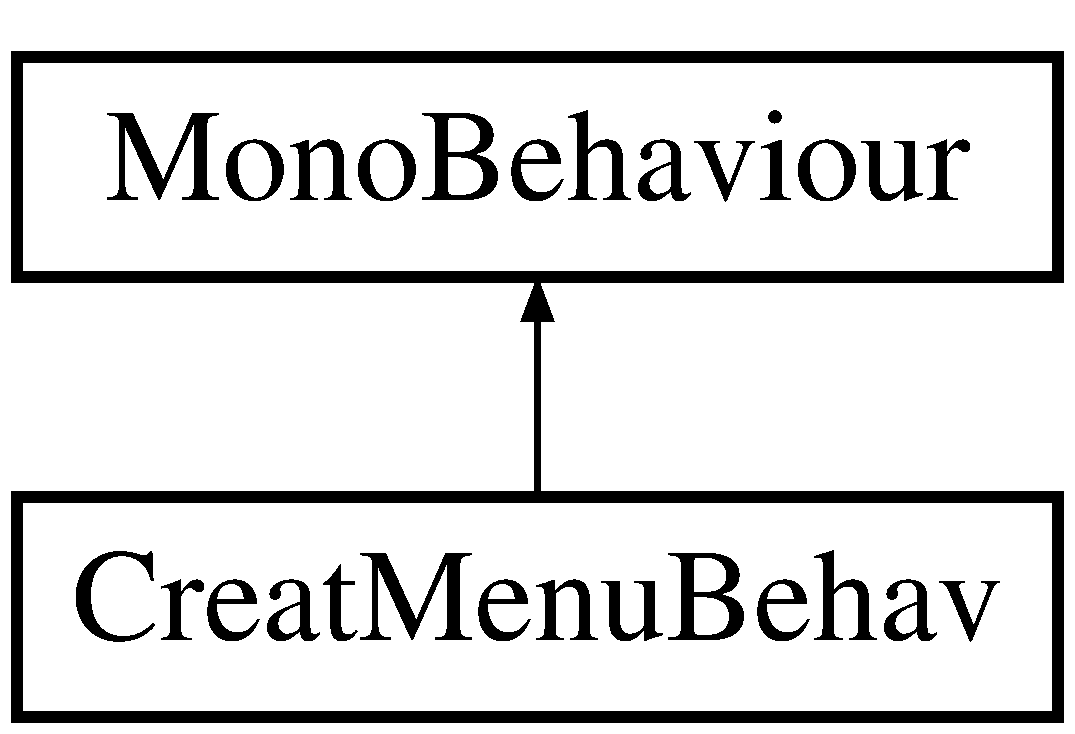
\includegraphics[height=2.000000cm]{class_creat_menu_behav}
\end{center}
\end{figure}
\subsection*{Public Member Functions}
\begin{DoxyCompactItemize}
\item 
void \mbox{\hyperlink{class_creat_menu_behav_a499eb1392e87f87a2acc080f00b4d2d5}{load\+Creat\+Menu}} (\mbox{\hyperlink{class_ecosystem_editor}{Ecosystem\+Editor}} ec)
\begin{DoxyCompactList}\small\item\em load the creature editor menu using the ecosystem editor \end{DoxyCompactList}\item 
void \mbox{\hyperlink{class_creat_menu_behav_a598bb35515126390ef8b93334b7c1044}{save\+Settings}} ()
\begin{DoxyCompactList}\small\item\em save the creature creator\textquotesingle{}s creature to the ecosystem \end{DoxyCompactList}\end{DoxyCompactItemize}
\subsection*{Public Attributes}
\begin{DoxyCompactItemize}
\item 
Game\+Object \mbox{\hyperlink{class_creat_menu_behav_a6fefbf26f7a00f949815efc0f6415cd5}{u\+I\+Parent}}
\end{DoxyCompactItemize}


\subsection{Member Function Documentation}
\mbox{\Hypertarget{class_creat_menu_behav_a499eb1392e87f87a2acc080f00b4d2d5}\label{class_creat_menu_behav_a499eb1392e87f87a2acc080f00b4d2d5}} 
\index{Creat\+Menu\+Behav@{Creat\+Menu\+Behav}!load\+Creat\+Menu@{load\+Creat\+Menu}}
\index{load\+Creat\+Menu@{load\+Creat\+Menu}!Creat\+Menu\+Behav@{Creat\+Menu\+Behav}}
\subsubsection{\texorpdfstring{load\+Creat\+Menu()}{loadCreatMenu()}}
{\footnotesize\ttfamily void Creat\+Menu\+Behav.\+load\+Creat\+Menu (\begin{DoxyParamCaption}\item[{\mbox{\hyperlink{class_ecosystem_editor}{Ecosystem\+Editor}}}]{ec }\end{DoxyParamCaption})}



load the creature editor menu using the ecosystem editor 

\mbox{\Hypertarget{class_creat_menu_behav_a598bb35515126390ef8b93334b7c1044}\label{class_creat_menu_behav_a598bb35515126390ef8b93334b7c1044}} 
\index{Creat\+Menu\+Behav@{Creat\+Menu\+Behav}!save\+Settings@{save\+Settings}}
\index{save\+Settings@{save\+Settings}!Creat\+Menu\+Behav@{Creat\+Menu\+Behav}}
\subsubsection{\texorpdfstring{save\+Settings()}{saveSettings()}}
{\footnotesize\ttfamily void Creat\+Menu\+Behav.\+save\+Settings (\begin{DoxyParamCaption}{ }\end{DoxyParamCaption})}



save the creature creator\textquotesingle{}s creature to the ecosystem 



\subsection{Member Data Documentation}
\mbox{\Hypertarget{class_creat_menu_behav_a6fefbf26f7a00f949815efc0f6415cd5}\label{class_creat_menu_behav_a6fefbf26f7a00f949815efc0f6415cd5}} 
\index{Creat\+Menu\+Behav@{Creat\+Menu\+Behav}!u\+I\+Parent@{u\+I\+Parent}}
\index{u\+I\+Parent@{u\+I\+Parent}!Creat\+Menu\+Behav@{Creat\+Menu\+Behav}}
\subsubsection{\texorpdfstring{u\+I\+Parent}{uIParent}}
{\footnotesize\ttfamily Game\+Object Creat\+Menu\+Behav.\+u\+I\+Parent}



The documentation for this class was generated from the following file\+:\begin{DoxyCompactItemize}
\item 
\mbox{\hyperlink{_creat_menu_behav_8cs}{Creat\+Menu\+Behav.\+cs}}\end{DoxyCompactItemize}

\hypertarget{class_creature}{}\section{Creature Class Reference}
\label{class_creature}\index{Creature@{Creature}}


Class for storing all data about a creature/agent, including its neural networks, queued actions, stored resources, location and other parameters.  


\subsection*{Public Member Functions}
\begin{DoxyCompactItemize}
\item 
\mbox{\hyperlink{class_creature_a33b98848ab1feddad8bf7badb46f8e57}{Creature}} (int max\+Ability\+Points)
\item 
\mbox{\hyperlink{class_creature_acd97b133e2a8f2fb38a7686ffd7a3fdc}{Creature}} ()
\item 
void \mbox{\hyperlink{class_creature_a84d61b231641c1af50195151ab904ada}{start\+Turn}} (\mbox{\hyperlink{class_ecosystem}{Ecosystem}} eco)
\begin{DoxyCompactList}\small\item\em Starts creatures turn \end{DoxyCompactList}\item 
void \mbox{\hyperlink{class_creature_a5c8e2c97a66f511939fc89bd349017d3}{add\+Actions\+To\+Queue}} ()
\item 
void \mbox{\hyperlink{class_creature_a46fa0cc06932a4cdba0e7b1f8f2dad9c}{print\+Networks}} ()
\item 
void \mbox{\hyperlink{class_creature_ad9f8df80e830988e67bf3eeeb016689c}{update\+Nets}} ()
\item 
void \mbox{\hyperlink{class_creature_aeaf23c7008fa80ca8897d13b5435e1fc}{update\+Neighbors}} ()
\begin{DoxyCompactList}\small\item\em Called at beginning of each turn. \end{DoxyCompactList}\item 
void \mbox{\hyperlink{class_creature_a372a0b61e98758214fddc2564dc649f2}{store\+Current\+Net\+State}} ()
\begin{DoxyCompactList}\small\item\em Stores the state of networks in prev\+Net\+States \end{DoxyCompactList}\item 
void \mbox{\hyperlink{class_creature_a4bdf06ee073ffb00f7410f791caaccdc}{perform\+Actions}} (\mbox{\hyperlink{class_ecosystem}{Ecosystem}} eco)
\begin{DoxyCompactList}\small\item\em Performs whatever actions in the queue it can. \end{DoxyCompactList}\item 
void \mbox{\hyperlink{class_creature_afa20bf76dd7678a5e60b75e2dadaa6ac}{resource\+Health\+Update}} ()
\begin{DoxyCompactList}\small\item\em Updates health based on resource levels. \end{DoxyCompactList}\item 
bool \mbox{\hyperlink{class_creature_a1938298b04f9a74b1692771a9f050478}{is\+Dead}} ()
\begin{DoxyCompactList}\small\item\em Returns true if health is 0 or below, also deletes creature from map if dead \end{DoxyCompactList}\item 
void \mbox{\hyperlink{class_creature_a617588216838f0fe3f8861f38c2746f2}{add\+Comm\+Networks}} ()
\begin{DoxyCompactList}\small\item\em Creates and adds comm networks to the first layer of \char`\"{}networks\char`\"{} using comm\+Signals, and comm\+Net\+Template \end{DoxyCompactList}\item 
int \mbox{\hyperlink{class_creature_aafecd84cf3b44bcb8dd67cd9518e3326}{add\+Network}} (int layer\+Of\+Nets)
\begin{DoxyCompactList}\small\item\em Adds network in given layer, and returns index of added layer. \end{DoxyCompactList}\item 
void \mbox{\hyperlink{class_creature_ab103ada400a5773ae0d34c11b3abf2d4}{send\+Comm\+Output\+Signals}} ()
\begin{DoxyCompactList}\small\item\em Iterates over neightbors and passes comm signals to them. \end{DoxyCompactList}\item 
void \mbox{\hyperlink{class_creature_a13b61e24bb6dfa9cd53e7919378c4b0c}{process\+Repro\+Requests}} ()
\begin{DoxyCompactList}\small\item\em process requests for reproduction. \end{DoxyCompactList}\item 
void \mbox{\hyperlink{class_creature_abd5e8fd01b4197fdb549fd38da914f2a}{reproduce}} (\mbox{\hyperlink{class_creature}{Creature}} mate)
\begin{DoxyCompactList}\small\item\em Reproduce with neighboring creature. \end{DoxyCompactList}\item 
void \mbox{\hyperlink{class_creature_a31a49fbd361a70ff3f1f41886519d0c5}{add\+Variation\+To\+Weights}} (float standard\+Dev)
\item 
\mbox{\hyperlink{class_creature}{Creature}} \mbox{\hyperlink{class_creature_a1095c7239ce30cb170ec739c343719fb}{get\+Shallow\+Copy}} ()
\end{DoxyCompactItemize}
\subsection*{Public Attributes}
\begin{DoxyCompactItemize}
\item 
\mbox{\hyperlink{class_creature}{Creature}} \mbox{\hyperlink{class_creature_ab689ebff012f90395825a404bd6990c6}{founder}}
\item 
\mbox{\hyperlink{class_land}{Land}} \mbox{\hyperlink{class_creature_a08982d1959e230238389a1a5e9853115}{dummy\+Land}} = new \mbox{\hyperlink{class_land}{Land}}()
\item 
int \mbox{\hyperlink{class_creature_a358feda4f0a406a8f28bed6acb170c37}{index}}
\item 
System.\+Random \mbox{\hyperlink{class_creature_ab3b01072caf7d87c396a2d80a3d73412}{rand}}
\item 
System.\+Random \mbox{\hyperlink{class_creature_a08184ad607f5105788e09e8501386da0}{rand2}}
\item 
Color \mbox{\hyperlink{class_creature_a4f2289e79c2db01559984c8797a322c8}{color}}
\item 
List$<$ Dictionary$<$ string, \mbox{\hyperlink{class_network}{Network}} $>$ $>$ \mbox{\hyperlink{class_creature_a1caf157811e3a3b37f9b292560aa0552}{networks}} = new List$<$Dictionary$<$string, \mbox{\hyperlink{class_network}{Network}}$>$$>$()
\begin{DoxyCompactList}\small\item\em Stores all networks into layers of lists of Networks. 10 Maximum \end{DoxyCompactList}\item 
string \mbox{\hyperlink{class_creature_a721fb38fcd0d2e7bfc307a6921e3fa2e}{species}} = \char`\"{}default\char`\"{}
\item 
List$<$ List$<$ \mbox{\hyperlink{class_land}{Land}} $>$ $>$ \mbox{\hyperlink{class_creature_ac96bc7e8b95322eeaadf280d715f738a}{map}}
\item 
int \mbox{[}$\,$\mbox{]} \mbox{\hyperlink{class_creature_ab6036649791244250e257da28733b2e7}{position}} = new int\mbox{[}2\mbox{]}
\item 
\mbox{\hyperlink{class_land}{Land}} \mbox{[}$\,$\mbox{]} \mbox{\hyperlink{class_creature_a6b427ac086b4cca5ed85553942e01d71}{neighbor\+Lands}} = new \mbox{\hyperlink{class_land}{Land}}\mbox{[}5\mbox{]}
\begin{DoxyCompactList}\small\item\em Neighbors are up, down, left, and right. Index 0 for land creature is on. \end{DoxyCompactList}\item 
Simple\+Priority\+Queue$<$ \mbox{\hyperlink{class_action}{Action}} $>$ \mbox{\hyperlink{class_creature_abb099197e9fa2dac396151e4e949214d}{action\+Queue}} = new Simple\+Priority\+Queue$<$\mbox{\hyperlink{class_action}{Action}}$>$()
\begin{DoxyCompactList}\small\item\em Actions to be taken by creature \end{DoxyCompactList}\item 
float \mbox{\hyperlink{class_creature_a8542dd67a39f6badb8e83e45e0fa4ff3}{remaining\+Turn\+Time}}
\begin{DoxyCompactList}\small\item\em Time remaining in turn\+: limits number of actions that can be taken in one turn. \end{DoxyCompactList}\item 
float \mbox{\hyperlink{class_creature_a7da8e444fb731af8e632b730d72e4215}{mutation\+Standard\+Deviation}}
\item 
float \mbox{\hyperlink{class_creature_a64066d7d20c1b74af7e2e8a5bd8e2410}{full\+Turn\+Time}}
\item 
int \mbox{\hyperlink{class_creature_a58383de337fb218495e70aa126981d6c}{num\+Layers\+Of\+Nets}}
\begin{DoxyCompactList}\small\item\em The number of layers of Networks \end{DoxyCompactList}\item 
List$<$ \mbox{\hyperlink{class_comm_signal}{Comm\+Signal}} $>$ \mbox{\hyperlink{class_creature_a1a6c6390564dda480623b55d89c6d5b3}{output\+Comm\+Signals}} = new List$<$\mbox{\hyperlink{class_comm_signal}{Comm\+Signal}}$>$()
\begin{DoxyCompactList}\small\item\em stores an array of booleans for each neighbor for communication. e.\+g. 8 neighbors by 3 bools each. \end{DoxyCompactList}\item 
List$<$ List$<$ Dictionary$<$ string, \mbox{\hyperlink{class_network}{Network}} $>$ $>$ $>$ \mbox{\hyperlink{class_creature_a36cd0e998e4f26599c6b31a54b5d30ac}{prev\+Net\+States}} = new List$<$List$<$Dictionary$<$string, \mbox{\hyperlink{class_network}{Network}}$>$$>$$>$()
\begin{DoxyCompactList}\small\item\em Not implememted yet. Stores the state of the networks for previous time steps. The front of the queue is the most recent network state (t-\/1). \end{DoxyCompactList}\item 
Dictionary$<$ string, \mbox{\hyperlink{class_ability}{Ability}} $>$ \mbox{\hyperlink{class_creature_a83af2d9bc8c0a8b819957c4029515b3f}{abilities}} = new Dictionary$<$string, \mbox{\hyperlink{class_ability}{Ability}}$>$()
\begin{DoxyCompactList}\small\item\em Designates which resources or species the creature has an advantage in consuming, attacking, or defending against. Certain combinations of excess resources can boost abilities. \end{DoxyCompactList}\item 
float \mbox{\hyperlink{class_creature_a3c0b32a41569e073d4dd717f25262d56}{health}}
\begin{DoxyCompactList}\small\item\em When health reaches zero, creature dies. \end{DoxyCompactList}\item 
Dictionary$<$ string, \mbox{\hyperlink{class_creature_resource}{Creature\+Resource}} $>$ \mbox{\hyperlink{class_creature_a1c4a7443dd2c8748ce3322b68914788a}{stored\+Resources}} = new Dictionary$<$string, \mbox{\hyperlink{class_creature_resource}{Creature\+Resource}}$>$()
\item 
bool \mbox{[}$\,$\mbox{]} \mbox{\hyperlink{class_creature_ae0d804e7589fe2c612dafe930d74fe46}{phenotype}}
\begin{DoxyCompactList}\small\item\em Outward appearance of creature\+: for communication purposes. Typically 4 bits. \end{DoxyCompactList}\item 
List$<$ \mbox{\hyperlink{class_comm_signal}{Comm\+Signal}} $>$ \mbox{\hyperlink{class_creature_a4051d02a4fb5ccb411e07cea92273a5a}{input\+Comm\+List}} = new List$<$\mbox{\hyperlink{class_comm_signal}{Comm\+Signal}}$>$()
\begin{DoxyCompactList}\small\item\em A list of incoming comm signals. \end{DoxyCompactList}\item 
\mbox{\hyperlink{class_comm_network}{Comm\+Network}} \mbox{\hyperlink{class_creature_a02c2c300201b3515e01e84766e4e02b9}{comm\+In\+Net\+Template}} = new \mbox{\hyperlink{class_comm_network}{Comm\+Network}}()
\begin{DoxyCompactList}\small\item\em A comm network will be created for each \mbox{\hyperlink{class_comm_signal}{Comm\+Signal}} in comm\+List, and added to the first layer of networks in \char`\"{}networks\char`\"{} (the input layer). \end{DoxyCompactList}\item 
\mbox{\hyperlink{class_comm_network}{Comm\+Network}} \mbox{\hyperlink{class_creature_ac17368a07178415519592669a89283bd}{comm\+Out\+Net\+Template}} = new \mbox{\hyperlink{class_comm_network}{Comm\+Network}}()
\begin{DoxyCompactList}\small\item\em A template for the network that generates actions towards a specific neighbor in response to comm input from that neighbor. \end{DoxyCompactList}\item 
float \mbox{\hyperlink{class_creature_ad894d0485d7bbd02a52893fe5d24a462}{max\+Health}}
\begin{DoxyCompactList}\small\item\em Maximum health that creature can attain. \end{DoxyCompactList}\item 
int \mbox{\hyperlink{class_creature_a52e3662ae3e269ee2cdc73b716fa3455}{remaining\+Ability\+Points}}
\item 
List$<$ \mbox{\hyperlink{class_repro_action}{Repro\+Action}} $>$ \mbox{\hyperlink{class_creature_a8df2df30dc7d2da9705159e6425208d9}{reproduction\+Requests}} = new List$<$\mbox{\hyperlink{class_repro_action}{Repro\+Action}}$>$()
\begin{DoxyCompactList}\small\item\em List of requests for reproduction from neighbors. \end{DoxyCompactList}\item 
\mbox{\hyperlink{class_repro_network}{Repro\+Network}} \mbox{\hyperlink{class_creature_a84614f4c93827ec6ba2754cd7cfa91e4}{reproduction\+Decider\+Network}} = new \mbox{\hyperlink{class_repro_network}{Repro\+Network}}()
\begin{DoxyCompactList}\small\item\em \mbox{\hyperlink{class_network}{Network}} to decide whether a creature should reproduce with a neightbor. \end{DoxyCompactList}\item 
Dictionary$<$ string, \mbox{\hyperlink{class_action}{Action}} $>$ \mbox{\hyperlink{class_creature_ab75f97aaea730b1da2bd00cc28555ac6}{action\+Pool}} = new Dictionary$<$string, \mbox{\hyperlink{class_action}{Action}}$>$()
\begin{DoxyCompactList}\small\item\em Dictionary of potential actions that the creature can take if assigned to an output node. \end{DoxyCompactList}\item 
int \mbox{\hyperlink{class_creature_a22b0a217ba84279341ad580b13080258}{action\+Clear\+Interval}} = 5
\item 
int \mbox{\hyperlink{class_creature_abb93da679575f5a4fb5c8072c831b7f0}{action\+Clear\+Count}} = 0
\item 
int \mbox{\hyperlink{class_creature_af4cfa9181ab0df58a2c64b6c3b9725f8}{action\+Clear\+Size}} = 10
\end{DoxyCompactItemize}


\subsection{Detailed Description}
Class for storing all data about a creature/agent, including its neural networks, queued actions, stored resources, location and other parameters. 



\subsection{Constructor \& Destructor Documentation}
\mbox{\Hypertarget{class_creature_a33b98848ab1feddad8bf7badb46f8e57}\label{class_creature_a33b98848ab1feddad8bf7badb46f8e57}} 
\index{Creature@{Creature}!Creature@{Creature}}
\index{Creature@{Creature}!Creature@{Creature}}
\subsubsection{\texorpdfstring{Creature()}{Creature()}\hspace{0.1cm}{\footnotesize\ttfamily [1/2]}}
{\footnotesize\ttfamily Creature.\+Creature (\begin{DoxyParamCaption}\item[{int}]{max\+Ability\+Points }\end{DoxyParamCaption})}

\mbox{\Hypertarget{class_creature_acd97b133e2a8f2fb38a7686ffd7a3fdc}\label{class_creature_acd97b133e2a8f2fb38a7686ffd7a3fdc}} 
\index{Creature@{Creature}!Creature@{Creature}}
\index{Creature@{Creature}!Creature@{Creature}}
\subsubsection{\texorpdfstring{Creature()}{Creature()}\hspace{0.1cm}{\footnotesize\ttfamily [2/2]}}
{\footnotesize\ttfamily Creature.\+Creature (\begin{DoxyParamCaption}{ }\end{DoxyParamCaption})}



\subsection{Member Function Documentation}
\mbox{\Hypertarget{class_creature_a5c8e2c97a66f511939fc89bd349017d3}\label{class_creature_a5c8e2c97a66f511939fc89bd349017d3}} 
\index{Creature@{Creature}!add\+Actions\+To\+Queue@{add\+Actions\+To\+Queue}}
\index{add\+Actions\+To\+Queue@{add\+Actions\+To\+Queue}!Creature@{Creature}}
\subsubsection{\texorpdfstring{add\+Actions\+To\+Queue()}{addActionsToQueue()}}
{\footnotesize\ttfamily void Creature.\+add\+Actions\+To\+Queue (\begin{DoxyParamCaption}{ }\end{DoxyParamCaption})}

\mbox{\Hypertarget{class_creature_a617588216838f0fe3f8861f38c2746f2}\label{class_creature_a617588216838f0fe3f8861f38c2746f2}} 
\index{Creature@{Creature}!add\+Comm\+Networks@{add\+Comm\+Networks}}
\index{add\+Comm\+Networks@{add\+Comm\+Networks}!Creature@{Creature}}
\subsubsection{\texorpdfstring{add\+Comm\+Networks()}{addCommNetworks()}}
{\footnotesize\ttfamily void Creature.\+add\+Comm\+Networks (\begin{DoxyParamCaption}{ }\end{DoxyParamCaption})}



Creates and adds comm networks to the first layer of \char`\"{}networks\char`\"{} using comm\+Signals, and comm\+Net\+Template 

\mbox{\Hypertarget{class_creature_aafecd84cf3b44bcb8dd67cd9518e3326}\label{class_creature_aafecd84cf3b44bcb8dd67cd9518e3326}} 
\index{Creature@{Creature}!add\+Network@{add\+Network}}
\index{add\+Network@{add\+Network}!Creature@{Creature}}
\subsubsection{\texorpdfstring{add\+Network()}{addNetwork()}}
{\footnotesize\ttfamily int Creature.\+add\+Network (\begin{DoxyParamCaption}\item[{int}]{layer\+Of\+Nets }\end{DoxyParamCaption})}



Adds network in given layer, and returns index of added layer. 


\begin{DoxyParams}{Parameters}
{\em layer\+Of\+Nets} & 0 to add to input nets, 1 to add to output nets.\\
\hline
\end{DoxyParams}
\mbox{\Hypertarget{class_creature_a31a49fbd361a70ff3f1f41886519d0c5}\label{class_creature_a31a49fbd361a70ff3f1f41886519d0c5}} 
\index{Creature@{Creature}!add\+Variation\+To\+Weights@{add\+Variation\+To\+Weights}}
\index{add\+Variation\+To\+Weights@{add\+Variation\+To\+Weights}!Creature@{Creature}}
\subsubsection{\texorpdfstring{add\+Variation\+To\+Weights()}{addVariationToWeights()}}
{\footnotesize\ttfamily void Creature.\+add\+Variation\+To\+Weights (\begin{DoxyParamCaption}\item[{float}]{standard\+Dev }\end{DoxyParamCaption})}

\mbox{\Hypertarget{class_creature_a1095c7239ce30cb170ec739c343719fb}\label{class_creature_a1095c7239ce30cb170ec739c343719fb}} 
\index{Creature@{Creature}!get\+Shallow\+Copy@{get\+Shallow\+Copy}}
\index{get\+Shallow\+Copy@{get\+Shallow\+Copy}!Creature@{Creature}}
\subsubsection{\texorpdfstring{get\+Shallow\+Copy()}{getShallowCopy()}}
{\footnotesize\ttfamily \mbox{\hyperlink{class_creature}{Creature}} Creature.\+get\+Shallow\+Copy (\begin{DoxyParamCaption}{ }\end{DoxyParamCaption})}

\mbox{\Hypertarget{class_creature_a1938298b04f9a74b1692771a9f050478}\label{class_creature_a1938298b04f9a74b1692771a9f050478}} 
\index{Creature@{Creature}!is\+Dead@{is\+Dead}}
\index{is\+Dead@{is\+Dead}!Creature@{Creature}}
\subsubsection{\texorpdfstring{is\+Dead()}{isDead()}}
{\footnotesize\ttfamily bool Creature.\+is\+Dead (\begin{DoxyParamCaption}{ }\end{DoxyParamCaption})}



Returns true if health is 0 or below, also deletes creature from map if dead 

\mbox{\Hypertarget{class_creature_a4bdf06ee073ffb00f7410f791caaccdc}\label{class_creature_a4bdf06ee073ffb00f7410f791caaccdc}} 
\index{Creature@{Creature}!perform\+Actions@{perform\+Actions}}
\index{perform\+Actions@{perform\+Actions}!Creature@{Creature}}
\subsubsection{\texorpdfstring{perform\+Actions()}{performActions()}}
{\footnotesize\ttfamily void Creature.\+perform\+Actions (\begin{DoxyParamCaption}\item[{\mbox{\hyperlink{class_ecosystem}{Ecosystem}}}]{eco }\end{DoxyParamCaption})}



Performs whatever actions in the queue it can. 

T\+O\+DO\+: allow for a certain number of actions to carry over, otherwise, only the first action put on the queue will be run each turn, which is biased\+: based on the order of the output nodes in the final layer one solution\+: sort the order in which output nodes are added to queue\mbox{\Hypertarget{class_creature_a46fa0cc06932a4cdba0e7b1f8f2dad9c}\label{class_creature_a46fa0cc06932a4cdba0e7b1f8f2dad9c}} 
\index{Creature@{Creature}!print\+Networks@{print\+Networks}}
\index{print\+Networks@{print\+Networks}!Creature@{Creature}}
\subsubsection{\texorpdfstring{print\+Networks()}{printNetworks()}}
{\footnotesize\ttfamily void Creature.\+print\+Networks (\begin{DoxyParamCaption}{ }\end{DoxyParamCaption})}

\mbox{\Hypertarget{class_creature_a13b61e24bb6dfa9cd53e7919378c4b0c}\label{class_creature_a13b61e24bb6dfa9cd53e7919378c4b0c}} 
\index{Creature@{Creature}!process\+Repro\+Requests@{process\+Repro\+Requests}}
\index{process\+Repro\+Requests@{process\+Repro\+Requests}!Creature@{Creature}}
\subsubsection{\texorpdfstring{process\+Repro\+Requests()}{processReproRequests()}}
{\footnotesize\ttfamily void Creature.\+process\+Repro\+Requests (\begin{DoxyParamCaption}{ }\end{DoxyParamCaption})}



process requests for reproduction. 

\mbox{\Hypertarget{class_creature_abd5e8fd01b4197fdb549fd38da914f2a}\label{class_creature_abd5e8fd01b4197fdb549fd38da914f2a}} 
\index{Creature@{Creature}!reproduce@{reproduce}}
\index{reproduce@{reproduce}!Creature@{Creature}}
\subsubsection{\texorpdfstring{reproduce()}{reproduce()}}
{\footnotesize\ttfamily void Creature.\+reproduce (\begin{DoxyParamCaption}\item[{\mbox{\hyperlink{class_creature}{Creature}}}]{mate }\end{DoxyParamCaption})}



Reproduce with neighboring creature. 


\begin{DoxyParams}{Parameters}
{\em mate} & \mbox{\hyperlink{class_creature}{Creature}} to reproduce with.\\
\hline
\end{DoxyParams}
\mbox{\Hypertarget{class_creature_afa20bf76dd7678a5e60b75e2dadaa6ac}\label{class_creature_afa20bf76dd7678a5e60b75e2dadaa6ac}} 
\index{Creature@{Creature}!resource\+Health\+Update@{resource\+Health\+Update}}
\index{resource\+Health\+Update@{resource\+Health\+Update}!Creature@{Creature}}
\subsubsection{\texorpdfstring{resource\+Health\+Update()}{resourceHealthUpdate()}}
{\footnotesize\ttfamily void Creature.\+resource\+Health\+Update (\begin{DoxyParamCaption}{ }\end{DoxyParamCaption})}



Updates health based on resource levels. 

\mbox{\Hypertarget{class_creature_ab103ada400a5773ae0d34c11b3abf2d4}\label{class_creature_ab103ada400a5773ae0d34c11b3abf2d4}} 
\index{Creature@{Creature}!send\+Comm\+Output\+Signals@{send\+Comm\+Output\+Signals}}
\index{send\+Comm\+Output\+Signals@{send\+Comm\+Output\+Signals}!Creature@{Creature}}
\subsubsection{\texorpdfstring{send\+Comm\+Output\+Signals()}{sendCommOutputSignals()}}
{\footnotesize\ttfamily void Creature.\+send\+Comm\+Output\+Signals (\begin{DoxyParamCaption}{ }\end{DoxyParamCaption})}



Iterates over neightbors and passes comm signals to them. 

\mbox{\Hypertarget{class_creature_a84d61b231641c1af50195151ab904ada}\label{class_creature_a84d61b231641c1af50195151ab904ada}} 
\index{Creature@{Creature}!start\+Turn@{start\+Turn}}
\index{start\+Turn@{start\+Turn}!Creature@{Creature}}
\subsubsection{\texorpdfstring{start\+Turn()}{startTurn()}}
{\footnotesize\ttfamily void Creature.\+start\+Turn (\begin{DoxyParamCaption}\item[{\mbox{\hyperlink{class_ecosystem}{Ecosystem}}}]{eco }\end{DoxyParamCaption})}



Starts creatures turn 

\mbox{\Hypertarget{class_creature_a372a0b61e98758214fddc2564dc649f2}\label{class_creature_a372a0b61e98758214fddc2564dc649f2}} 
\index{Creature@{Creature}!store\+Current\+Net\+State@{store\+Current\+Net\+State}}
\index{store\+Current\+Net\+State@{store\+Current\+Net\+State}!Creature@{Creature}}
\subsubsection{\texorpdfstring{store\+Current\+Net\+State()}{storeCurrentNetState()}}
{\footnotesize\ttfamily void Creature.\+store\+Current\+Net\+State (\begin{DoxyParamCaption}{ }\end{DoxyParamCaption})}



Stores the state of networks in prev\+Net\+States 

\mbox{\Hypertarget{class_creature_aeaf23c7008fa80ca8897d13b5435e1fc}\label{class_creature_aeaf23c7008fa80ca8897d13b5435e1fc}} 
\index{Creature@{Creature}!update\+Neighbors@{update\+Neighbors}}
\index{update\+Neighbors@{update\+Neighbors}!Creature@{Creature}}
\subsubsection{\texorpdfstring{update\+Neighbors()}{updateNeighbors()}}
{\footnotesize\ttfamily void Creature.\+update\+Neighbors (\begin{DoxyParamCaption}{ }\end{DoxyParamCaption})}



Called at beginning of each turn. 

\mbox{\Hypertarget{class_creature_ad9f8df80e830988e67bf3eeeb016689c}\label{class_creature_ad9f8df80e830988e67bf3eeeb016689c}} 
\index{Creature@{Creature}!update\+Nets@{update\+Nets}}
\index{update\+Nets@{update\+Nets}!Creature@{Creature}}
\subsubsection{\texorpdfstring{update\+Nets()}{updateNets()}}
{\footnotesize\ttfamily void Creature.\+update\+Nets (\begin{DoxyParamCaption}{ }\end{DoxyParamCaption})}



\subsection{Member Data Documentation}
\mbox{\Hypertarget{class_creature_a83af2d9bc8c0a8b819957c4029515b3f}\label{class_creature_a83af2d9bc8c0a8b819957c4029515b3f}} 
\index{Creature@{Creature}!abilities@{abilities}}
\index{abilities@{abilities}!Creature@{Creature}}
\subsubsection{\texorpdfstring{abilities}{abilities}}
{\footnotesize\ttfamily Dictionary$<$string, \mbox{\hyperlink{class_ability}{Ability}}$>$ Creature.\+abilities = new Dictionary$<$string, \mbox{\hyperlink{class_ability}{Ability}}$>$()}



Designates which resources or species the creature has an advantage in consuming, attacking, or defending against. Certain combinations of excess resources can boost abilities. 

\mbox{\Hypertarget{class_creature_abb93da679575f5a4fb5c8072c831b7f0}\label{class_creature_abb93da679575f5a4fb5c8072c831b7f0}} 
\index{Creature@{Creature}!action\+Clear\+Count@{action\+Clear\+Count}}
\index{action\+Clear\+Count@{action\+Clear\+Count}!Creature@{Creature}}
\subsubsection{\texorpdfstring{action\+Clear\+Count}{actionClearCount}}
{\footnotesize\ttfamily int Creature.\+action\+Clear\+Count = 0}

\mbox{\Hypertarget{class_creature_a22b0a217ba84279341ad580b13080258}\label{class_creature_a22b0a217ba84279341ad580b13080258}} 
\index{Creature@{Creature}!action\+Clear\+Interval@{action\+Clear\+Interval}}
\index{action\+Clear\+Interval@{action\+Clear\+Interval}!Creature@{Creature}}
\subsubsection{\texorpdfstring{action\+Clear\+Interval}{actionClearInterval}}
{\footnotesize\ttfamily int Creature.\+action\+Clear\+Interval = 5}

\mbox{\Hypertarget{class_creature_af4cfa9181ab0df58a2c64b6c3b9725f8}\label{class_creature_af4cfa9181ab0df58a2c64b6c3b9725f8}} 
\index{Creature@{Creature}!action\+Clear\+Size@{action\+Clear\+Size}}
\index{action\+Clear\+Size@{action\+Clear\+Size}!Creature@{Creature}}
\subsubsection{\texorpdfstring{action\+Clear\+Size}{actionClearSize}}
{\footnotesize\ttfamily int Creature.\+action\+Clear\+Size = 10}

\mbox{\Hypertarget{class_creature_ab75f97aaea730b1da2bd00cc28555ac6}\label{class_creature_ab75f97aaea730b1da2bd00cc28555ac6}} 
\index{Creature@{Creature}!action\+Pool@{action\+Pool}}
\index{action\+Pool@{action\+Pool}!Creature@{Creature}}
\subsubsection{\texorpdfstring{action\+Pool}{actionPool}}
{\footnotesize\ttfamily Dictionary$<$string, \mbox{\hyperlink{class_action}{Action}}$>$ Creature.\+action\+Pool = new Dictionary$<$string, \mbox{\hyperlink{class_action}{Action}}$>$()}



Dictionary of potential actions that the creature can take if assigned to an output node. 

\mbox{\Hypertarget{class_creature_abb099197e9fa2dac396151e4e949214d}\label{class_creature_abb099197e9fa2dac396151e4e949214d}} 
\index{Creature@{Creature}!action\+Queue@{action\+Queue}}
\index{action\+Queue@{action\+Queue}!Creature@{Creature}}
\subsubsection{\texorpdfstring{action\+Queue}{actionQueue}}
{\footnotesize\ttfamily Simple\+Priority\+Queue$<$\mbox{\hyperlink{class_action}{Action}}$>$ Creature.\+action\+Queue = new Simple\+Priority\+Queue$<$\mbox{\hyperlink{class_action}{Action}}$>$()}



Actions to be taken by creature 

\mbox{\Hypertarget{class_creature_a4f2289e79c2db01559984c8797a322c8}\label{class_creature_a4f2289e79c2db01559984c8797a322c8}} 
\index{Creature@{Creature}!color@{color}}
\index{color@{color}!Creature@{Creature}}
\subsubsection{\texorpdfstring{color}{color}}
{\footnotesize\ttfamily Color Creature.\+color}

\mbox{\Hypertarget{class_creature_a02c2c300201b3515e01e84766e4e02b9}\label{class_creature_a02c2c300201b3515e01e84766e4e02b9}} 
\index{Creature@{Creature}!comm\+In\+Net\+Template@{comm\+In\+Net\+Template}}
\index{comm\+In\+Net\+Template@{comm\+In\+Net\+Template}!Creature@{Creature}}
\subsubsection{\texorpdfstring{comm\+In\+Net\+Template}{commInNetTemplate}}
{\footnotesize\ttfamily \mbox{\hyperlink{class_comm_network}{Comm\+Network}} Creature.\+comm\+In\+Net\+Template = new \mbox{\hyperlink{class_comm_network}{Comm\+Network}}()}



A comm network will be created for each \mbox{\hyperlink{class_comm_signal}{Comm\+Signal}} in comm\+List, and added to the first layer of networks in \char`\"{}networks\char`\"{} (the input layer). 

\mbox{\Hypertarget{class_creature_ac17368a07178415519592669a89283bd}\label{class_creature_ac17368a07178415519592669a89283bd}} 
\index{Creature@{Creature}!comm\+Out\+Net\+Template@{comm\+Out\+Net\+Template}}
\index{comm\+Out\+Net\+Template@{comm\+Out\+Net\+Template}!Creature@{Creature}}
\subsubsection{\texorpdfstring{comm\+Out\+Net\+Template}{commOutNetTemplate}}
{\footnotesize\ttfamily \mbox{\hyperlink{class_comm_network}{Comm\+Network}} Creature.\+comm\+Out\+Net\+Template = new \mbox{\hyperlink{class_comm_network}{Comm\+Network}}()}



A template for the network that generates actions towards a specific neighbor in response to comm input from that neighbor. 

\mbox{\Hypertarget{class_creature_a08982d1959e230238389a1a5e9853115}\label{class_creature_a08982d1959e230238389a1a5e9853115}} 
\index{Creature@{Creature}!dummy\+Land@{dummy\+Land}}
\index{dummy\+Land@{dummy\+Land}!Creature@{Creature}}
\subsubsection{\texorpdfstring{dummy\+Land}{dummyLand}}
{\footnotesize\ttfamily \mbox{\hyperlink{class_land}{Land}} Creature.\+dummy\+Land = new \mbox{\hyperlink{class_land}{Land}}()}

\mbox{\Hypertarget{class_creature_ab689ebff012f90395825a404bd6990c6}\label{class_creature_ab689ebff012f90395825a404bd6990c6}} 
\index{Creature@{Creature}!founder@{founder}}
\index{founder@{founder}!Creature@{Creature}}
\subsubsection{\texorpdfstring{founder}{founder}}
{\footnotesize\ttfamily \mbox{\hyperlink{class_creature}{Creature}} Creature.\+founder}

\mbox{\Hypertarget{class_creature_a64066d7d20c1b74af7e2e8a5bd8e2410}\label{class_creature_a64066d7d20c1b74af7e2e8a5bd8e2410}} 
\index{Creature@{Creature}!full\+Turn\+Time@{full\+Turn\+Time}}
\index{full\+Turn\+Time@{full\+Turn\+Time}!Creature@{Creature}}
\subsubsection{\texorpdfstring{full\+Turn\+Time}{fullTurnTime}}
{\footnotesize\ttfamily float Creature.\+full\+Turn\+Time}

\mbox{\Hypertarget{class_creature_a3c0b32a41569e073d4dd717f25262d56}\label{class_creature_a3c0b32a41569e073d4dd717f25262d56}} 
\index{Creature@{Creature}!health@{health}}
\index{health@{health}!Creature@{Creature}}
\subsubsection{\texorpdfstring{health}{health}}
{\footnotesize\ttfamily float Creature.\+health}



When health reaches zero, creature dies. 

\mbox{\Hypertarget{class_creature_a358feda4f0a406a8f28bed6acb170c37}\label{class_creature_a358feda4f0a406a8f28bed6acb170c37}} 
\index{Creature@{Creature}!index@{index}}
\index{index@{index}!Creature@{Creature}}
\subsubsection{\texorpdfstring{index}{index}}
{\footnotesize\ttfamily int Creature.\+index}

\mbox{\Hypertarget{class_creature_a4051d02a4fb5ccb411e07cea92273a5a}\label{class_creature_a4051d02a4fb5ccb411e07cea92273a5a}} 
\index{Creature@{Creature}!input\+Comm\+List@{input\+Comm\+List}}
\index{input\+Comm\+List@{input\+Comm\+List}!Creature@{Creature}}
\subsubsection{\texorpdfstring{input\+Comm\+List}{inputCommList}}
{\footnotesize\ttfamily List$<$\mbox{\hyperlink{class_comm_signal}{Comm\+Signal}}$>$ Creature.\+input\+Comm\+List = new List$<$\mbox{\hyperlink{class_comm_signal}{Comm\+Signal}}$>$()}



A list of incoming comm signals. 

\mbox{\Hypertarget{class_creature_ac96bc7e8b95322eeaadf280d715f738a}\label{class_creature_ac96bc7e8b95322eeaadf280d715f738a}} 
\index{Creature@{Creature}!map@{map}}
\index{map@{map}!Creature@{Creature}}
\subsubsection{\texorpdfstring{map}{map}}
{\footnotesize\ttfamily List$<$List$<$\mbox{\hyperlink{class_land}{Land}}$>$ $>$ Creature.\+map}

\mbox{\Hypertarget{class_creature_ad894d0485d7bbd02a52893fe5d24a462}\label{class_creature_ad894d0485d7bbd02a52893fe5d24a462}} 
\index{Creature@{Creature}!max\+Health@{max\+Health}}
\index{max\+Health@{max\+Health}!Creature@{Creature}}
\subsubsection{\texorpdfstring{max\+Health}{maxHealth}}
{\footnotesize\ttfamily float Creature.\+max\+Health}



Maximum health that creature can attain. 

\mbox{\Hypertarget{class_creature_a7da8e444fb731af8e632b730d72e4215}\label{class_creature_a7da8e444fb731af8e632b730d72e4215}} 
\index{Creature@{Creature}!mutation\+Standard\+Deviation@{mutation\+Standard\+Deviation}}
\index{mutation\+Standard\+Deviation@{mutation\+Standard\+Deviation}!Creature@{Creature}}
\subsubsection{\texorpdfstring{mutation\+Standard\+Deviation}{mutationStandardDeviation}}
{\footnotesize\ttfamily float Creature.\+mutation\+Standard\+Deviation}

\mbox{\Hypertarget{class_creature_a6b427ac086b4cca5ed85553942e01d71}\label{class_creature_a6b427ac086b4cca5ed85553942e01d71}} 
\index{Creature@{Creature}!neighbor\+Lands@{neighbor\+Lands}}
\index{neighbor\+Lands@{neighbor\+Lands}!Creature@{Creature}}
\subsubsection{\texorpdfstring{neighbor\+Lands}{neighborLands}}
{\footnotesize\ttfamily \mbox{\hyperlink{class_land}{Land}} \mbox{[}$\,$\mbox{]} Creature.\+neighbor\+Lands = new \mbox{\hyperlink{class_land}{Land}}\mbox{[}5\mbox{]}}



Neighbors are up, down, left, and right. Index 0 for land creature is on. 

\mbox{\Hypertarget{class_creature_a1caf157811e3a3b37f9b292560aa0552}\label{class_creature_a1caf157811e3a3b37f9b292560aa0552}} 
\index{Creature@{Creature}!networks@{networks}}
\index{networks@{networks}!Creature@{Creature}}
\subsubsection{\texorpdfstring{networks}{networks}}
{\footnotesize\ttfamily List$<$Dictionary$<$string, \mbox{\hyperlink{class_network}{Network}}$>$ $>$ Creature.\+networks = new List$<$Dictionary$<$string, \mbox{\hyperlink{class_network}{Network}}$>$$>$()}



Stores all networks into layers of lists of Networks. 10 Maximum 

\mbox{\Hypertarget{class_creature_a58383de337fb218495e70aa126981d6c}\label{class_creature_a58383de337fb218495e70aa126981d6c}} 
\index{Creature@{Creature}!num\+Layers\+Of\+Nets@{num\+Layers\+Of\+Nets}}
\index{num\+Layers\+Of\+Nets@{num\+Layers\+Of\+Nets}!Creature@{Creature}}
\subsubsection{\texorpdfstring{num\+Layers\+Of\+Nets}{numLayersOfNets}}
{\footnotesize\ttfamily int Creature.\+num\+Layers\+Of\+Nets}



The number of layers of Networks 

\mbox{\Hypertarget{class_creature_a1a6c6390564dda480623b55d89c6d5b3}\label{class_creature_a1a6c6390564dda480623b55d89c6d5b3}} 
\index{Creature@{Creature}!output\+Comm\+Signals@{output\+Comm\+Signals}}
\index{output\+Comm\+Signals@{output\+Comm\+Signals}!Creature@{Creature}}
\subsubsection{\texorpdfstring{output\+Comm\+Signals}{outputCommSignals}}
{\footnotesize\ttfamily List$<$\mbox{\hyperlink{class_comm_signal}{Comm\+Signal}}$>$ Creature.\+output\+Comm\+Signals = new List$<$\mbox{\hyperlink{class_comm_signal}{Comm\+Signal}}$>$()}



stores an array of booleans for each neighbor for communication. e.\+g. 8 neighbors by 3 bools each. 

\mbox{\Hypertarget{class_creature_ae0d804e7589fe2c612dafe930d74fe46}\label{class_creature_ae0d804e7589fe2c612dafe930d74fe46}} 
\index{Creature@{Creature}!phenotype@{phenotype}}
\index{phenotype@{phenotype}!Creature@{Creature}}
\subsubsection{\texorpdfstring{phenotype}{phenotype}}
{\footnotesize\ttfamily bool \mbox{[}$\,$\mbox{]} Creature.\+phenotype}



Outward appearance of creature\+: for communication purposes. Typically 4 bits. 

\mbox{\Hypertarget{class_creature_ab6036649791244250e257da28733b2e7}\label{class_creature_ab6036649791244250e257da28733b2e7}} 
\index{Creature@{Creature}!position@{position}}
\index{position@{position}!Creature@{Creature}}
\subsubsection{\texorpdfstring{position}{position}}
{\footnotesize\ttfamily int \mbox{[}$\,$\mbox{]} Creature.\+position = new int\mbox{[}2\mbox{]}}

\mbox{\Hypertarget{class_creature_a36cd0e998e4f26599c6b31a54b5d30ac}\label{class_creature_a36cd0e998e4f26599c6b31a54b5d30ac}} 
\index{Creature@{Creature}!prev\+Net\+States@{prev\+Net\+States}}
\index{prev\+Net\+States@{prev\+Net\+States}!Creature@{Creature}}
\subsubsection{\texorpdfstring{prev\+Net\+States}{prevNetStates}}
{\footnotesize\ttfamily List$<$List$<$Dictionary$<$string, \mbox{\hyperlink{class_network}{Network}}$>$ $>$ $>$ Creature.\+prev\+Net\+States = new List$<$List$<$Dictionary$<$string, \mbox{\hyperlink{class_network}{Network}}$>$$>$$>$()}



Not implememted yet. Stores the state of the networks for previous time steps. The front of the queue is the most recent network state (t-\/1). 

\mbox{\Hypertarget{class_creature_ab3b01072caf7d87c396a2d80a3d73412}\label{class_creature_ab3b01072caf7d87c396a2d80a3d73412}} 
\index{Creature@{Creature}!rand@{rand}}
\index{rand@{rand}!Creature@{Creature}}
\subsubsection{\texorpdfstring{rand}{rand}}
{\footnotesize\ttfamily System.\+Random Creature.\+rand}

\mbox{\Hypertarget{class_creature_a08184ad607f5105788e09e8501386da0}\label{class_creature_a08184ad607f5105788e09e8501386da0}} 
\index{Creature@{Creature}!rand2@{rand2}}
\index{rand2@{rand2}!Creature@{Creature}}
\subsubsection{\texorpdfstring{rand2}{rand2}}
{\footnotesize\ttfamily System.\+Random Creature.\+rand2}

\mbox{\Hypertarget{class_creature_a52e3662ae3e269ee2cdc73b716fa3455}\label{class_creature_a52e3662ae3e269ee2cdc73b716fa3455}} 
\index{Creature@{Creature}!remaining\+Ability\+Points@{remaining\+Ability\+Points}}
\index{remaining\+Ability\+Points@{remaining\+Ability\+Points}!Creature@{Creature}}
\subsubsection{\texorpdfstring{remaining\+Ability\+Points}{remainingAbilityPoints}}
{\footnotesize\ttfamily int Creature.\+remaining\+Ability\+Points}

\mbox{\Hypertarget{class_creature_a8542dd67a39f6badb8e83e45e0fa4ff3}\label{class_creature_a8542dd67a39f6badb8e83e45e0fa4ff3}} 
\index{Creature@{Creature}!remaining\+Turn\+Time@{remaining\+Turn\+Time}}
\index{remaining\+Turn\+Time@{remaining\+Turn\+Time}!Creature@{Creature}}
\subsubsection{\texorpdfstring{remaining\+Turn\+Time}{remainingTurnTime}}
{\footnotesize\ttfamily float Creature.\+remaining\+Turn\+Time}



Time remaining in turn\+: limits number of actions that can be taken in one turn. 

\mbox{\Hypertarget{class_creature_a84614f4c93827ec6ba2754cd7cfa91e4}\label{class_creature_a84614f4c93827ec6ba2754cd7cfa91e4}} 
\index{Creature@{Creature}!reproduction\+Decider\+Network@{reproduction\+Decider\+Network}}
\index{reproduction\+Decider\+Network@{reproduction\+Decider\+Network}!Creature@{Creature}}
\subsubsection{\texorpdfstring{reproduction\+Decider\+Network}{reproductionDeciderNetwork}}
{\footnotesize\ttfamily \mbox{\hyperlink{class_repro_network}{Repro\+Network}} Creature.\+reproduction\+Decider\+Network = new \mbox{\hyperlink{class_repro_network}{Repro\+Network}}()}



\mbox{\hyperlink{class_network}{Network}} to decide whether a creature should reproduce with a neightbor. 

\mbox{\Hypertarget{class_creature_a8df2df30dc7d2da9705159e6425208d9}\label{class_creature_a8df2df30dc7d2da9705159e6425208d9}} 
\index{Creature@{Creature}!reproduction\+Requests@{reproduction\+Requests}}
\index{reproduction\+Requests@{reproduction\+Requests}!Creature@{Creature}}
\subsubsection{\texorpdfstring{reproduction\+Requests}{reproductionRequests}}
{\footnotesize\ttfamily List$<$\mbox{\hyperlink{class_repro_action}{Repro\+Action}}$>$ Creature.\+reproduction\+Requests = new List$<$\mbox{\hyperlink{class_repro_action}{Repro\+Action}}$>$()}



List of requests for reproduction from neighbors. 

\mbox{\Hypertarget{class_creature_a721fb38fcd0d2e7bfc307a6921e3fa2e}\label{class_creature_a721fb38fcd0d2e7bfc307a6921e3fa2e}} 
\index{Creature@{Creature}!species@{species}}
\index{species@{species}!Creature@{Creature}}
\subsubsection{\texorpdfstring{species}{species}}
{\footnotesize\ttfamily string Creature.\+species = \char`\"{}default\char`\"{}}

\mbox{\Hypertarget{class_creature_a1c4a7443dd2c8748ce3322b68914788a}\label{class_creature_a1c4a7443dd2c8748ce3322b68914788a}} 
\index{Creature@{Creature}!stored\+Resources@{stored\+Resources}}
\index{stored\+Resources@{stored\+Resources}!Creature@{Creature}}
\subsubsection{\texorpdfstring{stored\+Resources}{storedResources}}
{\footnotesize\ttfamily Dictionary$<$string, \mbox{\hyperlink{class_creature_resource}{Creature\+Resource}}$>$ Creature.\+stored\+Resources = new Dictionary$<$string, \mbox{\hyperlink{class_creature_resource}{Creature\+Resource}}$>$()}



The documentation for this class was generated from the following file\+:\begin{DoxyCompactItemize}
\item 
\mbox{\hyperlink{_creature_8cs}{Creature.\+cs}}\end{DoxyCompactItemize}

\hypertarget{class_creature_editor}{}\section{Creature\+Editor Class Reference}
\label{class_creature_editor}\index{Creature\+Editor@{Creature\+Editor}}
\subsection*{Public Member Functions}
\begin{DoxyCompactItemize}
\item 
\mbox{\hyperlink{class_creature_editor_ad25258b45808b5e140dd76aa7eec7b29}{Creature\+Editor}} (\mbox{\hyperlink{class_creature}{Creature}} \mbox{\hyperlink{class_creature_editor_a2589284f2064a318bd8578acb95f3309}{creature}}, \mbox{\hyperlink{class_ecosystem_editor}{Ecosystem\+Editor}} eco\+Creator)
\begin{DoxyCompactList}\small\item\em Constructor \end{DoxyCompactList}\item 
void \mbox{\hyperlink{class_creature_editor_a25dc6294586118bf7e4ecefeccea2815}{set\+Species}} (string species)
\begin{DoxyCompactList}\small\item\em Sets name of species to which the creature belongs. \end{DoxyCompactList}\item 
void \mbox{\hyperlink{class_creature_editor_af2c3731115defa893138dcb7de00092c}{set\+Position}} (int x\+Coor, int y\+Coor)
\begin{DoxyCompactList}\small\item\em Sets creature\textquotesingle{}s position on the map. \end{DoxyCompactList}\item 
void \mbox{\hyperlink{class_creature_editor_a2a1426689b7276996e550e5c508e9a48}{set\+Max\+Health}} (float max\+Health)
\item 
void \mbox{\hyperlink{class_creature_editor_a2a230941e6db58928582e20704a8d239}{set\+Initial\+Health}} (float initial\+Health)
\item 
void \mbox{\hyperlink{class_creature_editor_a0ef7391c366e987d267d7ba937447146}{set\+Color}} (\mbox{\hyperlink{_creature_editor_8cs_a2d31a955c823bd51aec8f913e263723c}{Color\+Choice}} c)
\item 
void \mbox{\hyperlink{class_creature_editor_a63a9951aa74689237e12cd131cef6e0e}{set\+Phenotype}} (int phenotype)
\begin{DoxyCompactList}\small\item\em Sets phenotype of creature. Takes in int\+: \mbox{[}1,x\mbox{]}, where there are x distinct phenotypes allowed in the ecosystem, and assigns corrresponding bool array to creatures phenotype. The bool array contains all falses, except for a true at the x-\/1 index. \end{DoxyCompactList}\item 
void \mbox{\hyperlink{class_creature_editor_a1dec102cd9c1c32e2f0639a627203c7f}{set\+Action\+Clear\+Interval}} (int steps)
\begin{DoxyCompactList}\small\item\em Sets the number of steps between deleting all actions in action queue. This is used to keep the action queue current. \end{DoxyCompactList}\item 
void \mbox{\hyperlink{class_creature_editor_a463412404c7ed5f27208b742318f193d}{set\+Action\+Clear\+Size}} (int size)
\begin{DoxyCompactList}\small\item\em Sets the size of the action queue required for the queue to be cleared \end{DoxyCompactList}\item 
void \mbox{\hyperlink{class_creature_editor_aeebb715ee7340999be80095aeb6c5c41}{set\+Mutation\+Standard\+Deviation}} (float deviation)
\begin{DoxyCompactList}\small\item\em Sets the amount of deviation added to the weights during reproduction \end{DoxyCompactList}\item 
void \mbox{\hyperlink{class_creature_editor_a89072895132cbeae88d530bada8c0761}{set\+Turn\+Time}} (float time)
\begin{DoxyCompactList}\small\item\em Sets the amount of time alloted per turn. \end{DoxyCompactList}\item 
\mbox{\hyperlink{class_resource_editor}{Resource\+Editor}} \mbox{\hyperlink{class_creature_editor_a6cd78de22a211b236369afe62ea60c99}{add\+Resource}} ()
\begin{DoxyCompactList}\small\item\em Resets creatures resource creator, allowing the user to create a resource for the creature to use for survival or attribute benefits. \end{DoxyCompactList}\item 
void \mbox{\hyperlink{class_creature_editor_af35082ae3f97f9385b6d27efb1528e7c}{save\+Resource}} ()
\begin{DoxyCompactList}\small\item\em Saves resource created by resource creator. \end{DoxyCompactList}\item 
\mbox{\hyperlink{class_abilities_editor}{Abilities\+Editor}} \mbox{\hyperlink{class_creature_editor_a60b1083bafbb24636e356f2ca79e91b7}{edit\+Abilities}} ()
\begin{DoxyCompactList}\small\item\em edit tentative\+Abilities, returns Abilites\+Editor \end{DoxyCompactList}\item 
void \mbox{\hyperlink{class_creature_editor_afc80714657aedc32aaaa54760bc6b78f}{cancel\+Editing\+Abilities}} ()
\begin{DoxyCompactList}\small\item\em reset tentative\+Abilities if user cancels editing them \end{DoxyCompactList}\item 
void \mbox{\hyperlink{class_creature_editor_a73b06f4546ad17a435f487a3a515e661}{add\+Default\+Resource\+Abilities}} ()
\item 
\mbox{\hyperlink{class_network_editor}{Network\+Editor}} \mbox{\hyperlink{class_creature_editor_a2c3d33249073a6af3cd536cc02832635}{add\+Network}} ()
\begin{DoxyCompactList}\small\item\em Resets net\+Creator, allowing for the creation of a new network. \end{DoxyCompactList}\item 
\mbox{\hyperlink{class_action_editor}{Action\+Editor}} \mbox{\hyperlink{class_creature_editor_a558b61296fbae7699cfafdcc02bd8858}{add\+Action}} ()
\item 
void \mbox{\hyperlink{class_creature_editor_a4f9898932327b32b8eaedd8667acff18}{save\+Action}} ()
\item 
void \mbox{\hyperlink{class_creature_editor_a30e7e56df84510ae8487df6b62dc7f2a}{save\+Network}} ()
\begin{DoxyCompactList}\small\item\em Used to save network that is created by Net\+Creator. \end{DoxyCompactList}\item 
void \mbox{\hyperlink{class_creature_editor_a986bfbfe3b55a2b6492e1b4b371cf592}{save\+Abilities}} ()
\begin{DoxyCompactList}\small\item\em Saves abilities set by abilities creator. \end{DoxyCompactList}\item 
void \mbox{\hyperlink{class_creature_editor_a1d2e73a7a581c8e1e6c25c46ad8c8ace}{generate\+Default\+Action\+Pool}} ()
\end{DoxyCompactItemize}
\subsection*{Public Attributes}
\begin{DoxyCompactItemize}
\item 
\mbox{\hyperlink{class_creature}{Creature}} \mbox{\hyperlink{class_creature_editor_a2589284f2064a318bd8578acb95f3309}{creature}}
\item 
\mbox{\hyperlink{class_network_editor}{Network\+Editor}} \mbox{\hyperlink{class_creature_editor_ae6f73bff56b148123b3ca5251bb00aee}{net\+Creator}}
\item 
\mbox{\hyperlink{class_resource_editor}{Resource\+Editor}} \mbox{\hyperlink{class_creature_editor_a61c343493865d7ead92c5ea83fdfe6f5}{resource\+Creator}}
\item 
\mbox{\hyperlink{class_abilities_editor}{Abilities\+Editor}} \mbox{\hyperlink{class_creature_editor_a801504d4a32e2ad56c4c1ffda29d75f6}{abilities\+Creator}}
\item 
\mbox{\hyperlink{class_action_editor}{Action\+Editor}} \mbox{\hyperlink{class_creature_editor_a2bd48e758a2f1db48ad15d765debf5f2}{action\+Creator}}
\item 
int \mbox{\hyperlink{class_creature_editor_af48eb3267dc56b717ed3ba596794a362}{distinct\+Phenotypes}}
\end{DoxyCompactItemize}


\subsection{Detailed Description}
A\+PI for creature class. Stored by Ecosystem\+Creator.

\subsection{Constructor \& Destructor Documentation}
\mbox{\Hypertarget{class_creature_editor_ad25258b45808b5e140dd76aa7eec7b29}\label{class_creature_editor_ad25258b45808b5e140dd76aa7eec7b29}} 
\index{Creature\+Editor@{Creature\+Editor}!Creature\+Editor@{Creature\+Editor}}
\index{Creature\+Editor@{Creature\+Editor}!Creature\+Editor@{Creature\+Editor}}
\subsubsection{\texorpdfstring{Creature\+Editor()}{CreatureEditor()}}
{\footnotesize\ttfamily Creature\+Editor.\+Creature\+Editor (\begin{DoxyParamCaption}\item[{\mbox{\hyperlink{class_creature}{Creature}}}]{creature,  }\item[{\mbox{\hyperlink{class_ecosystem_editor}{Ecosystem\+Editor}}}]{eco\+Creator }\end{DoxyParamCaption})}



Constructor 



\subsection{Member Function Documentation}
\mbox{\Hypertarget{class_creature_editor_a558b61296fbae7699cfafdcc02bd8858}\label{class_creature_editor_a558b61296fbae7699cfafdcc02bd8858}} 
\index{Creature\+Editor@{Creature\+Editor}!add\+Action@{add\+Action}}
\index{add\+Action@{add\+Action}!Creature\+Editor@{Creature\+Editor}}
\subsubsection{\texorpdfstring{add\+Action()}{addAction()}}
{\footnotesize\ttfamily \mbox{\hyperlink{class_action_editor}{Action\+Editor}} Creature\+Editor.\+add\+Action (\begin{DoxyParamCaption}{ }\end{DoxyParamCaption})}

\mbox{\Hypertarget{class_creature_editor_a73b06f4546ad17a435f487a3a515e661}\label{class_creature_editor_a73b06f4546ad17a435f487a3a515e661}} 
\index{Creature\+Editor@{Creature\+Editor}!add\+Default\+Resource\+Abilities@{add\+Default\+Resource\+Abilities}}
\index{add\+Default\+Resource\+Abilities@{add\+Default\+Resource\+Abilities}!Creature\+Editor@{Creature\+Editor}}
\subsubsection{\texorpdfstring{add\+Default\+Resource\+Abilities()}{addDefaultResourceAbilities()}}
{\footnotesize\ttfamily void Creature\+Editor.\+add\+Default\+Resource\+Abilities (\begin{DoxyParamCaption}{ }\end{DoxyParamCaption})}

\mbox{\Hypertarget{class_creature_editor_a2c3d33249073a6af3cd536cc02832635}\label{class_creature_editor_a2c3d33249073a6af3cd536cc02832635}} 
\index{Creature\+Editor@{Creature\+Editor}!add\+Network@{add\+Network}}
\index{add\+Network@{add\+Network}!Creature\+Editor@{Creature\+Editor}}
\subsubsection{\texorpdfstring{add\+Network()}{addNetwork()}}
{\footnotesize\ttfamily \mbox{\hyperlink{class_network_editor}{Network\+Editor}} Creature\+Editor.\+add\+Network (\begin{DoxyParamCaption}{ }\end{DoxyParamCaption})}



Resets net\+Creator, allowing for the creation of a new network. 

\mbox{\Hypertarget{class_creature_editor_a6cd78de22a211b236369afe62ea60c99}\label{class_creature_editor_a6cd78de22a211b236369afe62ea60c99}} 
\index{Creature\+Editor@{Creature\+Editor}!add\+Resource@{add\+Resource}}
\index{add\+Resource@{add\+Resource}!Creature\+Editor@{Creature\+Editor}}
\subsubsection{\texorpdfstring{add\+Resource()}{addResource()}}
{\footnotesize\ttfamily \mbox{\hyperlink{class_resource_editor}{Resource\+Editor}} Creature\+Editor.\+add\+Resource (\begin{DoxyParamCaption}{ }\end{DoxyParamCaption})}



Resets creatures resource creator, allowing the user to create a resource for the creature to use for survival or attribute benefits. 

\mbox{\Hypertarget{class_creature_editor_afc80714657aedc32aaaa54760bc6b78f}\label{class_creature_editor_afc80714657aedc32aaaa54760bc6b78f}} 
\index{Creature\+Editor@{Creature\+Editor}!cancel\+Editing\+Abilities@{cancel\+Editing\+Abilities}}
\index{cancel\+Editing\+Abilities@{cancel\+Editing\+Abilities}!Creature\+Editor@{Creature\+Editor}}
\subsubsection{\texorpdfstring{cancel\+Editing\+Abilities()}{cancelEditingAbilities()}}
{\footnotesize\ttfamily void Creature\+Editor.\+cancel\+Editing\+Abilities (\begin{DoxyParamCaption}{ }\end{DoxyParamCaption})}



reset tentative\+Abilities if user cancels editing them 

\mbox{\Hypertarget{class_creature_editor_a60b1083bafbb24636e356f2ca79e91b7}\label{class_creature_editor_a60b1083bafbb24636e356f2ca79e91b7}} 
\index{Creature\+Editor@{Creature\+Editor}!edit\+Abilities@{edit\+Abilities}}
\index{edit\+Abilities@{edit\+Abilities}!Creature\+Editor@{Creature\+Editor}}
\subsubsection{\texorpdfstring{edit\+Abilities()}{editAbilities()}}
{\footnotesize\ttfamily \mbox{\hyperlink{class_abilities_editor}{Abilities\+Editor}} Creature\+Editor.\+edit\+Abilities (\begin{DoxyParamCaption}{ }\end{DoxyParamCaption})}



edit tentative\+Abilities, returns Abilites\+Editor 

\mbox{\Hypertarget{class_creature_editor_a1d2e73a7a581c8e1e6c25c46ad8c8ace}\label{class_creature_editor_a1d2e73a7a581c8e1e6c25c46ad8c8ace}} 
\index{Creature\+Editor@{Creature\+Editor}!generate\+Default\+Action\+Pool@{generate\+Default\+Action\+Pool}}
\index{generate\+Default\+Action\+Pool@{generate\+Default\+Action\+Pool}!Creature\+Editor@{Creature\+Editor}}
\subsubsection{\texorpdfstring{generate\+Default\+Action\+Pool()}{generateDefaultActionPool()}}
{\footnotesize\ttfamily void Creature\+Editor.\+generate\+Default\+Action\+Pool (\begin{DoxyParamCaption}{ }\end{DoxyParamCaption})}

\mbox{\Hypertarget{class_creature_editor_a986bfbfe3b55a2b6492e1b4b371cf592}\label{class_creature_editor_a986bfbfe3b55a2b6492e1b4b371cf592}} 
\index{Creature\+Editor@{Creature\+Editor}!save\+Abilities@{save\+Abilities}}
\index{save\+Abilities@{save\+Abilities}!Creature\+Editor@{Creature\+Editor}}
\subsubsection{\texorpdfstring{save\+Abilities()}{saveAbilities()}}
{\footnotesize\ttfamily void Creature\+Editor.\+save\+Abilities (\begin{DoxyParamCaption}{ }\end{DoxyParamCaption})}



Saves abilities set by abilities creator. 

\mbox{\Hypertarget{class_creature_editor_a4f9898932327b32b8eaedd8667acff18}\label{class_creature_editor_a4f9898932327b32b8eaedd8667acff18}} 
\index{Creature\+Editor@{Creature\+Editor}!save\+Action@{save\+Action}}
\index{save\+Action@{save\+Action}!Creature\+Editor@{Creature\+Editor}}
\subsubsection{\texorpdfstring{save\+Action()}{saveAction()}}
{\footnotesize\ttfamily void Creature\+Editor.\+save\+Action (\begin{DoxyParamCaption}{ }\end{DoxyParamCaption})}

\mbox{\Hypertarget{class_creature_editor_a30e7e56df84510ae8487df6b62dc7f2a}\label{class_creature_editor_a30e7e56df84510ae8487df6b62dc7f2a}} 
\index{Creature\+Editor@{Creature\+Editor}!save\+Network@{save\+Network}}
\index{save\+Network@{save\+Network}!Creature\+Editor@{Creature\+Editor}}
\subsubsection{\texorpdfstring{save\+Network()}{saveNetwork()}}
{\footnotesize\ttfamily void Creature\+Editor.\+save\+Network (\begin{DoxyParamCaption}{ }\end{DoxyParamCaption})}



Used to save network that is created by Net\+Creator. 

\mbox{\Hypertarget{class_creature_editor_af35082ae3f97f9385b6d27efb1528e7c}\label{class_creature_editor_af35082ae3f97f9385b6d27efb1528e7c}} 
\index{Creature\+Editor@{Creature\+Editor}!save\+Resource@{save\+Resource}}
\index{save\+Resource@{save\+Resource}!Creature\+Editor@{Creature\+Editor}}
\subsubsection{\texorpdfstring{save\+Resource()}{saveResource()}}
{\footnotesize\ttfamily void Creature\+Editor.\+save\+Resource (\begin{DoxyParamCaption}{ }\end{DoxyParamCaption})}



Saves resource created by resource creator. 

\mbox{\Hypertarget{class_creature_editor_a1dec102cd9c1c32e2f0639a627203c7f}\label{class_creature_editor_a1dec102cd9c1c32e2f0639a627203c7f}} 
\index{Creature\+Editor@{Creature\+Editor}!set\+Action\+Clear\+Interval@{set\+Action\+Clear\+Interval}}
\index{set\+Action\+Clear\+Interval@{set\+Action\+Clear\+Interval}!Creature\+Editor@{Creature\+Editor}}
\subsubsection{\texorpdfstring{set\+Action\+Clear\+Interval()}{setActionClearInterval()}}
{\footnotesize\ttfamily void Creature\+Editor.\+set\+Action\+Clear\+Interval (\begin{DoxyParamCaption}\item[{int}]{steps }\end{DoxyParamCaption})}



Sets the number of steps between deleting all actions in action queue. This is used to keep the action queue current. 

\mbox{\Hypertarget{class_creature_editor_a463412404c7ed5f27208b742318f193d}\label{class_creature_editor_a463412404c7ed5f27208b742318f193d}} 
\index{Creature\+Editor@{Creature\+Editor}!set\+Action\+Clear\+Size@{set\+Action\+Clear\+Size}}
\index{set\+Action\+Clear\+Size@{set\+Action\+Clear\+Size}!Creature\+Editor@{Creature\+Editor}}
\subsubsection{\texorpdfstring{set\+Action\+Clear\+Size()}{setActionClearSize()}}
{\footnotesize\ttfamily void Creature\+Editor.\+set\+Action\+Clear\+Size (\begin{DoxyParamCaption}\item[{int}]{size }\end{DoxyParamCaption})}



Sets the size of the action queue required for the queue to be cleared 

\mbox{\Hypertarget{class_creature_editor_a0ef7391c366e987d267d7ba937447146}\label{class_creature_editor_a0ef7391c366e987d267d7ba937447146}} 
\index{Creature\+Editor@{Creature\+Editor}!set\+Color@{set\+Color}}
\index{set\+Color@{set\+Color}!Creature\+Editor@{Creature\+Editor}}
\subsubsection{\texorpdfstring{set\+Color()}{setColor()}}
{\footnotesize\ttfamily void Creature\+Editor.\+set\+Color (\begin{DoxyParamCaption}\item[{\mbox{\hyperlink{_creature_editor_8cs_a2d31a955c823bd51aec8f913e263723c}{Color\+Choice}}}]{c }\end{DoxyParamCaption})}

\mbox{\Hypertarget{class_creature_editor_a2a230941e6db58928582e20704a8d239}\label{class_creature_editor_a2a230941e6db58928582e20704a8d239}} 
\index{Creature\+Editor@{Creature\+Editor}!set\+Initial\+Health@{set\+Initial\+Health}}
\index{set\+Initial\+Health@{set\+Initial\+Health}!Creature\+Editor@{Creature\+Editor}}
\subsubsection{\texorpdfstring{set\+Initial\+Health()}{setInitialHealth()}}
{\footnotesize\ttfamily void Creature\+Editor.\+set\+Initial\+Health (\begin{DoxyParamCaption}\item[{float}]{initial\+Health }\end{DoxyParamCaption})}

\mbox{\Hypertarget{class_creature_editor_a2a1426689b7276996e550e5c508e9a48}\label{class_creature_editor_a2a1426689b7276996e550e5c508e9a48}} 
\index{Creature\+Editor@{Creature\+Editor}!set\+Max\+Health@{set\+Max\+Health}}
\index{set\+Max\+Health@{set\+Max\+Health}!Creature\+Editor@{Creature\+Editor}}
\subsubsection{\texorpdfstring{set\+Max\+Health()}{setMaxHealth()}}
{\footnotesize\ttfamily void Creature\+Editor.\+set\+Max\+Health (\begin{DoxyParamCaption}\item[{float}]{max\+Health }\end{DoxyParamCaption})}

\mbox{\Hypertarget{class_creature_editor_aeebb715ee7340999be80095aeb6c5c41}\label{class_creature_editor_aeebb715ee7340999be80095aeb6c5c41}} 
\index{Creature\+Editor@{Creature\+Editor}!set\+Mutation\+Standard\+Deviation@{set\+Mutation\+Standard\+Deviation}}
\index{set\+Mutation\+Standard\+Deviation@{set\+Mutation\+Standard\+Deviation}!Creature\+Editor@{Creature\+Editor}}
\subsubsection{\texorpdfstring{set\+Mutation\+Standard\+Deviation()}{setMutationStandardDeviation()}}
{\footnotesize\ttfamily void Creature\+Editor.\+set\+Mutation\+Standard\+Deviation (\begin{DoxyParamCaption}\item[{float}]{deviation }\end{DoxyParamCaption})}



Sets the amount of deviation added to the weights during reproduction 

\mbox{\Hypertarget{class_creature_editor_a63a9951aa74689237e12cd131cef6e0e}\label{class_creature_editor_a63a9951aa74689237e12cd131cef6e0e}} 
\index{Creature\+Editor@{Creature\+Editor}!set\+Phenotype@{set\+Phenotype}}
\index{set\+Phenotype@{set\+Phenotype}!Creature\+Editor@{Creature\+Editor}}
\subsubsection{\texorpdfstring{set\+Phenotype()}{setPhenotype()}}
{\footnotesize\ttfamily void Creature\+Editor.\+set\+Phenotype (\begin{DoxyParamCaption}\item[{int}]{phenotype }\end{DoxyParamCaption})}



Sets phenotype of creature. Takes in int\+: \mbox{[}1,x\mbox{]}, where there are x distinct phenotypes allowed in the ecosystem, and assigns corrresponding bool array to creatures phenotype. The bool array contains all falses, except for a true at the x-\/1 index. 


\begin{DoxyParams}{Parameters}
{\em phenotype} & Must be 1 -\/ x\+: Where there are x distinct phenotypes allowed in the ecosystem (set in \mbox{\hyperlink{class_ecosystem}{Ecosystem}} class).\\
\hline
\end{DoxyParams}
\mbox{\Hypertarget{class_creature_editor_af2c3731115defa893138dcb7de00092c}\label{class_creature_editor_af2c3731115defa893138dcb7de00092c}} 
\index{Creature\+Editor@{Creature\+Editor}!set\+Position@{set\+Position}}
\index{set\+Position@{set\+Position}!Creature\+Editor@{Creature\+Editor}}
\subsubsection{\texorpdfstring{set\+Position()}{setPosition()}}
{\footnotesize\ttfamily void Creature\+Editor.\+set\+Position (\begin{DoxyParamCaption}\item[{int}]{x\+Coor,  }\item[{int}]{y\+Coor }\end{DoxyParamCaption})}



Sets creature\textquotesingle{}s position on the map. 

\mbox{\Hypertarget{class_creature_editor_a25dc6294586118bf7e4ecefeccea2815}\label{class_creature_editor_a25dc6294586118bf7e4ecefeccea2815}} 
\index{Creature\+Editor@{Creature\+Editor}!set\+Species@{set\+Species}}
\index{set\+Species@{set\+Species}!Creature\+Editor@{Creature\+Editor}}
\subsubsection{\texorpdfstring{set\+Species()}{setSpecies()}}
{\footnotesize\ttfamily void Creature\+Editor.\+set\+Species (\begin{DoxyParamCaption}\item[{string}]{species }\end{DoxyParamCaption})}



Sets name of species to which the creature belongs. 

\mbox{\Hypertarget{class_creature_editor_a89072895132cbeae88d530bada8c0761}\label{class_creature_editor_a89072895132cbeae88d530bada8c0761}} 
\index{Creature\+Editor@{Creature\+Editor}!set\+Turn\+Time@{set\+Turn\+Time}}
\index{set\+Turn\+Time@{set\+Turn\+Time}!Creature\+Editor@{Creature\+Editor}}
\subsubsection{\texorpdfstring{set\+Turn\+Time()}{setTurnTime()}}
{\footnotesize\ttfamily void Creature\+Editor.\+set\+Turn\+Time (\begin{DoxyParamCaption}\item[{float}]{time }\end{DoxyParamCaption})}



Sets the amount of time alloted per turn. 



\subsection{Member Data Documentation}
\mbox{\Hypertarget{class_creature_editor_a801504d4a32e2ad56c4c1ffda29d75f6}\label{class_creature_editor_a801504d4a32e2ad56c4c1ffda29d75f6}} 
\index{Creature\+Editor@{Creature\+Editor}!abilities\+Creator@{abilities\+Creator}}
\index{abilities\+Creator@{abilities\+Creator}!Creature\+Editor@{Creature\+Editor}}
\subsubsection{\texorpdfstring{abilities\+Creator}{abilitiesCreator}}
{\footnotesize\ttfamily \mbox{\hyperlink{class_abilities_editor}{Abilities\+Editor}} Creature\+Editor.\+abilities\+Creator}

\mbox{\Hypertarget{class_creature_editor_a2bd48e758a2f1db48ad15d765debf5f2}\label{class_creature_editor_a2bd48e758a2f1db48ad15d765debf5f2}} 
\index{Creature\+Editor@{Creature\+Editor}!action\+Creator@{action\+Creator}}
\index{action\+Creator@{action\+Creator}!Creature\+Editor@{Creature\+Editor}}
\subsubsection{\texorpdfstring{action\+Creator}{actionCreator}}
{\footnotesize\ttfamily \mbox{\hyperlink{class_action_editor}{Action\+Editor}} Creature\+Editor.\+action\+Creator}

\mbox{\Hypertarget{class_creature_editor_a2589284f2064a318bd8578acb95f3309}\label{class_creature_editor_a2589284f2064a318bd8578acb95f3309}} 
\index{Creature\+Editor@{Creature\+Editor}!creature@{creature}}
\index{creature@{creature}!Creature\+Editor@{Creature\+Editor}}
\subsubsection{\texorpdfstring{creature}{creature}}
{\footnotesize\ttfamily \mbox{\hyperlink{class_creature}{Creature}} Creature\+Editor.\+creature}

\mbox{\Hypertarget{class_creature_editor_af48eb3267dc56b717ed3ba596794a362}\label{class_creature_editor_af48eb3267dc56b717ed3ba596794a362}} 
\index{Creature\+Editor@{Creature\+Editor}!distinct\+Phenotypes@{distinct\+Phenotypes}}
\index{distinct\+Phenotypes@{distinct\+Phenotypes}!Creature\+Editor@{Creature\+Editor}}
\subsubsection{\texorpdfstring{distinct\+Phenotypes}{distinctPhenotypes}}
{\footnotesize\ttfamily int Creature\+Editor.\+distinct\+Phenotypes}

\mbox{\Hypertarget{class_creature_editor_ae6f73bff56b148123b3ca5251bb00aee}\label{class_creature_editor_ae6f73bff56b148123b3ca5251bb00aee}} 
\index{Creature\+Editor@{Creature\+Editor}!net\+Creator@{net\+Creator}}
\index{net\+Creator@{net\+Creator}!Creature\+Editor@{Creature\+Editor}}
\subsubsection{\texorpdfstring{net\+Creator}{netCreator}}
{\footnotesize\ttfamily \mbox{\hyperlink{class_network_editor}{Network\+Editor}} Creature\+Editor.\+net\+Creator}

\mbox{\Hypertarget{class_creature_editor_a61c343493865d7ead92c5ea83fdfe6f5}\label{class_creature_editor_a61c343493865d7ead92c5ea83fdfe6f5}} 
\index{Creature\+Editor@{Creature\+Editor}!resource\+Creator@{resource\+Creator}}
\index{resource\+Creator@{resource\+Creator}!Creature\+Editor@{Creature\+Editor}}
\subsubsection{\texorpdfstring{resource\+Creator}{resourceCreator}}
{\footnotesize\ttfamily \mbox{\hyperlink{class_resource_editor}{Resource\+Editor}} Creature\+Editor.\+resource\+Creator}



The documentation for this class was generated from the following file\+:\begin{DoxyCompactItemize}
\item 
\mbox{\hyperlink{_creature_editor_8cs}{Creature\+Editor.\+cs}}\end{DoxyCompactItemize}

\hypertarget{class_creature_resource}{}\section{Creature\+Resource Class Reference}
\label{class_creature_resource}\index{Creature\+Resource@{Creature\+Resource}}


Resource stored by a creature, and how that resource effects the creature.  


\subsection*{Public Member Functions}
\begin{DoxyCompactItemize}
\item 
void \mbox{\hyperlink{class_creature_resource_ae5678920b5302ad56650bdaec0fde5e5}{health\+Update}} (\mbox{\hyperlink{class_creature}{Creature}} creature)
\begin{DoxyCompactList}\small\item\em Update creature health according to resource level. \end{DoxyCompactList}\item 
\mbox{\hyperlink{class_creature_resource}{Creature\+Resource}} \mbox{\hyperlink{class_creature_resource_a994286201a611ddfada1fced56e427e7}{get\+Shallow\+Copy}} ()
\end{DoxyCompactItemize}
\subsection*{Public Attributes}
\begin{DoxyCompactItemize}
\item 
float \mbox{\hyperlink{class_creature_resource_a1d8ce8cdf8414b708970f1e3c6742715}{deficiency\+Threshold}}
\begin{DoxyCompactList}\small\item\em Threshold below which resource causes health damage. \end{DoxyCompactList}\item 
float \mbox{\hyperlink{class_creature_resource_a3d2bf29f213887c3d85882ab71bf941c}{deficiency\+Health\+Drain}}
\begin{DoxyCompactList}\small\item\em Amount of health drain from deficiency in one time step. \end{DoxyCompactList}\item 
float \mbox{\hyperlink{class_creature_resource_a588a6af5013d944441028c859ab6cabe}{current\+Level}}
\begin{DoxyCompactList}\small\item\em Amount of the resource currently stored. \end{DoxyCompactList}\item 
float \mbox{\hyperlink{class_creature_resource_a6aaa2e2cde79ab61cbf3683eccc2abff}{health\+Gain}}
\begin{DoxyCompactList}\small\item\em Amount of health gained when resource is adequate. \end{DoxyCompactList}\item 
float \mbox{\hyperlink{class_creature_resource_a2c4cc459420f7200685c9f0978a63116}{health\+Gain\+Threshold}}
\begin{DoxyCompactList}\small\item\em Threshold above which health is gained. \end{DoxyCompactList}\item 
float \mbox{\hyperlink{class_creature_resource_ac971dcddb000d950d2bfe414e4a5ca7b}{max\+Level}}
\item 
float \mbox{\hyperlink{class_creature_resource_a6ed5ee9d74de65191323bd6bfd5764e5}{base\+Usage}}
\item 
string \mbox{\hyperlink{class_creature_resource_a4653faf953fa8384caf57e2b47893d3a}{name}}
\end{DoxyCompactItemize}


\subsection{Detailed Description}
Resource stored by a creature, and how that resource effects the creature. 



\subsection{Member Function Documentation}
\mbox{\Hypertarget{class_creature_resource_a994286201a611ddfada1fced56e427e7}\label{class_creature_resource_a994286201a611ddfada1fced56e427e7}} 
\index{Creature\+Resource@{Creature\+Resource}!get\+Shallow\+Copy@{get\+Shallow\+Copy}}
\index{get\+Shallow\+Copy@{get\+Shallow\+Copy}!Creature\+Resource@{Creature\+Resource}}
\subsubsection{\texorpdfstring{get\+Shallow\+Copy()}{getShallowCopy()}}
{\footnotesize\ttfamily \mbox{\hyperlink{class_creature_resource}{Creature\+Resource}} Creature\+Resource.\+get\+Shallow\+Copy (\begin{DoxyParamCaption}{ }\end{DoxyParamCaption})}

\mbox{\Hypertarget{class_creature_resource_ae5678920b5302ad56650bdaec0fde5e5}\label{class_creature_resource_ae5678920b5302ad56650bdaec0fde5e5}} 
\index{Creature\+Resource@{Creature\+Resource}!health\+Update@{health\+Update}}
\index{health\+Update@{health\+Update}!Creature\+Resource@{Creature\+Resource}}
\subsubsection{\texorpdfstring{health\+Update()}{healthUpdate()}}
{\footnotesize\ttfamily void Creature\+Resource.\+health\+Update (\begin{DoxyParamCaption}\item[{\mbox{\hyperlink{class_creature}{Creature}}}]{creature }\end{DoxyParamCaption})}



Update creature health according to resource level. 



\subsection{Member Data Documentation}
\mbox{\Hypertarget{class_creature_resource_a6ed5ee9d74de65191323bd6bfd5764e5}\label{class_creature_resource_a6ed5ee9d74de65191323bd6bfd5764e5}} 
\index{Creature\+Resource@{Creature\+Resource}!base\+Usage@{base\+Usage}}
\index{base\+Usage@{base\+Usage}!Creature\+Resource@{Creature\+Resource}}
\subsubsection{\texorpdfstring{base\+Usage}{baseUsage}}
{\footnotesize\ttfamily float Creature\+Resource.\+base\+Usage}

\mbox{\Hypertarget{class_creature_resource_a588a6af5013d944441028c859ab6cabe}\label{class_creature_resource_a588a6af5013d944441028c859ab6cabe}} 
\index{Creature\+Resource@{Creature\+Resource}!current\+Level@{current\+Level}}
\index{current\+Level@{current\+Level}!Creature\+Resource@{Creature\+Resource}}
\subsubsection{\texorpdfstring{current\+Level}{currentLevel}}
{\footnotesize\ttfamily float Creature\+Resource.\+current\+Level}



Amount of the resource currently stored. 

\mbox{\Hypertarget{class_creature_resource_a3d2bf29f213887c3d85882ab71bf941c}\label{class_creature_resource_a3d2bf29f213887c3d85882ab71bf941c}} 
\index{Creature\+Resource@{Creature\+Resource}!deficiency\+Health\+Drain@{deficiency\+Health\+Drain}}
\index{deficiency\+Health\+Drain@{deficiency\+Health\+Drain}!Creature\+Resource@{Creature\+Resource}}
\subsubsection{\texorpdfstring{deficiency\+Health\+Drain}{deficiencyHealthDrain}}
{\footnotesize\ttfamily float Creature\+Resource.\+deficiency\+Health\+Drain}



Amount of health drain from deficiency in one time step. 

\mbox{\Hypertarget{class_creature_resource_a1d8ce8cdf8414b708970f1e3c6742715}\label{class_creature_resource_a1d8ce8cdf8414b708970f1e3c6742715}} 
\index{Creature\+Resource@{Creature\+Resource}!deficiency\+Threshold@{deficiency\+Threshold}}
\index{deficiency\+Threshold@{deficiency\+Threshold}!Creature\+Resource@{Creature\+Resource}}
\subsubsection{\texorpdfstring{deficiency\+Threshold}{deficiencyThreshold}}
{\footnotesize\ttfamily float Creature\+Resource.\+deficiency\+Threshold}



Threshold below which resource causes health damage. 

\mbox{\Hypertarget{class_creature_resource_a6aaa2e2cde79ab61cbf3683eccc2abff}\label{class_creature_resource_a6aaa2e2cde79ab61cbf3683eccc2abff}} 
\index{Creature\+Resource@{Creature\+Resource}!health\+Gain@{health\+Gain}}
\index{health\+Gain@{health\+Gain}!Creature\+Resource@{Creature\+Resource}}
\subsubsection{\texorpdfstring{health\+Gain}{healthGain}}
{\footnotesize\ttfamily float Creature\+Resource.\+health\+Gain}



Amount of health gained when resource is adequate. 

\mbox{\Hypertarget{class_creature_resource_a2c4cc459420f7200685c9f0978a63116}\label{class_creature_resource_a2c4cc459420f7200685c9f0978a63116}} 
\index{Creature\+Resource@{Creature\+Resource}!health\+Gain\+Threshold@{health\+Gain\+Threshold}}
\index{health\+Gain\+Threshold@{health\+Gain\+Threshold}!Creature\+Resource@{Creature\+Resource}}
\subsubsection{\texorpdfstring{health\+Gain\+Threshold}{healthGainThreshold}}
{\footnotesize\ttfamily float Creature\+Resource.\+health\+Gain\+Threshold}



Threshold above which health is gained. 

\mbox{\Hypertarget{class_creature_resource_ac971dcddb000d950d2bfe414e4a5ca7b}\label{class_creature_resource_ac971dcddb000d950d2bfe414e4a5ca7b}} 
\index{Creature\+Resource@{Creature\+Resource}!max\+Level@{max\+Level}}
\index{max\+Level@{max\+Level}!Creature\+Resource@{Creature\+Resource}}
\subsubsection{\texorpdfstring{max\+Level}{maxLevel}}
{\footnotesize\ttfamily float Creature\+Resource.\+max\+Level}

\mbox{\Hypertarget{class_creature_resource_a4653faf953fa8384caf57e2b47893d3a}\label{class_creature_resource_a4653faf953fa8384caf57e2b47893d3a}} 
\index{Creature\+Resource@{Creature\+Resource}!name@{name}}
\index{name@{name}!Creature\+Resource@{Creature\+Resource}}
\subsubsection{\texorpdfstring{name}{name}}
{\footnotesize\ttfamily string Creature\+Resource.\+name}



The documentation for this class was generated from the following file\+:\begin{DoxyCompactItemize}
\item 
\mbox{\hyperlink{_creature_resource_8cs}{Creature\+Resource.\+cs}}\end{DoxyCompactItemize}

\hypertarget{class_eco_manager}{}\section{Eco\+Manager Class Reference}
\label{class_eco_manager}\index{Eco\+Manager@{Eco\+Manager}}
\subsection*{Public Member Functions}
\begin{DoxyCompactItemize}
\item 
void \mbox{\hyperlink{class_eco_manager_ab7ee9ad1b41a4dbb9c8cb5f4c001e469}{make\+Eco}} ()
\item 
void \mbox{\hyperlink{class_eco_manager_a14997719023cc4431bf3b8ee2339163d}{user\+Creates\+Ecosystem}} (int map\+Width)
\item 
void \mbox{\hyperlink{class_eco_manager_ae6ddbd7e4c1fe49dafdf9cf72e121563}{user\+Adds\+Species}} (string name, \mbox{\hyperlink{_creature_editor_8cs_a2d31a955c823bd51aec8f913e263723c}{Color\+Choice}} color, float mutation\+Deviation)
\item 
void \mbox{\hyperlink{class_eco_manager_afff509be31e995fff88fd410bb96899f}{user\+Populates\+Species}} (string name, float population\+Deviation, int pop\+Size, int max\+Pop\+Size)
\item 
void \mbox{\hyperlink{class_eco_manager_a83ca906cad37e9a2c6e41bc58e638e2e}{run\+System}} (int steps)
\item 
\mbox{\hyperlink{class_ecosystem}{Ecosystem}} \mbox{\hyperlink{class_eco_manager_ac4afac929280d605388d110a4a0a2840}{get\+Ecosystem}} ()
\item 
void \mbox{\hyperlink{class_eco_manager_a7f08416b1570f58d235093da6d2c2129}{make\+Sensory\+Input\+Node}} (\mbox{\hyperlink{class_network_editor}{Network\+Editor}} net\+Creator, int land\+Index, string sensed\+Resource)
\item 
void \mbox{\hyperlink{class_eco_manager_a4d84a2362550dc39724e36df7d30ad06}{make\+Output\+Node}} (\mbox{\hyperlink{class_network_editor}{Network\+Editor}} net\+Creator, \mbox{\hyperlink{_non_input_node_8cs_a832a6943e91e304dea9608c4ae2818e7}{Activation\+Behavior\+Types}} activation\+Type, string action, int layer)
\item 
void \mbox{\hyperlink{class_eco_manager_a01ca1dd0c8bb417a67cbb83fe84b894d}{make\+Inner\+Input\+Node}} (\mbox{\hyperlink{class_network_editor}{Network\+Editor}} net\+Creator, int layer, string linked\+Net\+Name, int linked\+Net\+Index, int linked\+Node\+Index)
\end{DoxyCompactItemize}


\subsection{Member Function Documentation}
\mbox{\Hypertarget{class_eco_manager_ac4afac929280d605388d110a4a0a2840}\label{class_eco_manager_ac4afac929280d605388d110a4a0a2840}} 
\index{Eco\+Manager@{Eco\+Manager}!get\+Ecosystem@{get\+Ecosystem}}
\index{get\+Ecosystem@{get\+Ecosystem}!Eco\+Manager@{Eco\+Manager}}
\subsubsection{\texorpdfstring{get\+Ecosystem()}{getEcosystem()}}
{\footnotesize\ttfamily \mbox{\hyperlink{class_ecosystem}{Ecosystem}} Eco\+Manager.\+get\+Ecosystem (\begin{DoxyParamCaption}{ }\end{DoxyParamCaption})}

\mbox{\Hypertarget{class_eco_manager_ab7ee9ad1b41a4dbb9c8cb5f4c001e469}\label{class_eco_manager_ab7ee9ad1b41a4dbb9c8cb5f4c001e469}} 
\index{Eco\+Manager@{Eco\+Manager}!make\+Eco@{make\+Eco}}
\index{make\+Eco@{make\+Eco}!Eco\+Manager@{Eco\+Manager}}
\subsubsection{\texorpdfstring{make\+Eco()}{makeEco()}}
{\footnotesize\ttfamily void Eco\+Manager.\+make\+Eco (\begin{DoxyParamCaption}{ }\end{DoxyParamCaption})}

\mbox{\Hypertarget{class_eco_manager_a01ca1dd0c8bb417a67cbb83fe84b894d}\label{class_eco_manager_a01ca1dd0c8bb417a67cbb83fe84b894d}} 
\index{Eco\+Manager@{Eco\+Manager}!make\+Inner\+Input\+Node@{make\+Inner\+Input\+Node}}
\index{make\+Inner\+Input\+Node@{make\+Inner\+Input\+Node}!Eco\+Manager@{Eco\+Manager}}
\subsubsection{\texorpdfstring{make\+Inner\+Input\+Node()}{makeInnerInputNode()}}
{\footnotesize\ttfamily void Eco\+Manager.\+make\+Inner\+Input\+Node (\begin{DoxyParamCaption}\item[{\mbox{\hyperlink{class_network_editor}{Network\+Editor}}}]{net\+Creator,  }\item[{int}]{layer,  }\item[{string}]{linked\+Net\+Name,  }\item[{int}]{linked\+Net\+Index,  }\item[{int}]{linked\+Node\+Index }\end{DoxyParamCaption})}

\mbox{\Hypertarget{class_eco_manager_a4d84a2362550dc39724e36df7d30ad06}\label{class_eco_manager_a4d84a2362550dc39724e36df7d30ad06}} 
\index{Eco\+Manager@{Eco\+Manager}!make\+Output\+Node@{make\+Output\+Node}}
\index{make\+Output\+Node@{make\+Output\+Node}!Eco\+Manager@{Eco\+Manager}}
\subsubsection{\texorpdfstring{make\+Output\+Node()}{makeOutputNode()}}
{\footnotesize\ttfamily void Eco\+Manager.\+make\+Output\+Node (\begin{DoxyParamCaption}\item[{\mbox{\hyperlink{class_network_editor}{Network\+Editor}}}]{net\+Creator,  }\item[{\mbox{\hyperlink{_non_input_node_8cs_a832a6943e91e304dea9608c4ae2818e7}{Activation\+Behavior\+Types}}}]{activation\+Type,  }\item[{string}]{action,  }\item[{int}]{layer }\end{DoxyParamCaption})}

\mbox{\Hypertarget{class_eco_manager_a7f08416b1570f58d235093da6d2c2129}\label{class_eco_manager_a7f08416b1570f58d235093da6d2c2129}} 
\index{Eco\+Manager@{Eco\+Manager}!make\+Sensory\+Input\+Node@{make\+Sensory\+Input\+Node}}
\index{make\+Sensory\+Input\+Node@{make\+Sensory\+Input\+Node}!Eco\+Manager@{Eco\+Manager}}
\subsubsection{\texorpdfstring{make\+Sensory\+Input\+Node()}{makeSensoryInputNode()}}
{\footnotesize\ttfamily void Eco\+Manager.\+make\+Sensory\+Input\+Node (\begin{DoxyParamCaption}\item[{\mbox{\hyperlink{class_network_editor}{Network\+Editor}}}]{net\+Creator,  }\item[{int}]{land\+Index,  }\item[{string}]{sensed\+Resource }\end{DoxyParamCaption})}

\mbox{\Hypertarget{class_eco_manager_a83ca906cad37e9a2c6e41bc58e638e2e}\label{class_eco_manager_a83ca906cad37e9a2c6e41bc58e638e2e}} 
\index{Eco\+Manager@{Eco\+Manager}!run\+System@{run\+System}}
\index{run\+System@{run\+System}!Eco\+Manager@{Eco\+Manager}}
\subsubsection{\texorpdfstring{run\+System()}{runSystem()}}
{\footnotesize\ttfamily void Eco\+Manager.\+run\+System (\begin{DoxyParamCaption}\item[{int}]{steps }\end{DoxyParamCaption})}

\mbox{\Hypertarget{class_eco_manager_ae6ddbd7e4c1fe49dafdf9cf72e121563}\label{class_eco_manager_ae6ddbd7e4c1fe49dafdf9cf72e121563}} 
\index{Eco\+Manager@{Eco\+Manager}!user\+Adds\+Species@{user\+Adds\+Species}}
\index{user\+Adds\+Species@{user\+Adds\+Species}!Eco\+Manager@{Eco\+Manager}}
\subsubsection{\texorpdfstring{user\+Adds\+Species()}{userAddsSpecies()}}
{\footnotesize\ttfamily void Eco\+Manager.\+user\+Adds\+Species (\begin{DoxyParamCaption}\item[{string}]{name,  }\item[{\mbox{\hyperlink{_creature_editor_8cs_a2d31a955c823bd51aec8f913e263723c}{Color\+Choice}}}]{color,  }\item[{float}]{mutation\+Deviation }\end{DoxyParamCaption})}

\mbox{\Hypertarget{class_eco_manager_a14997719023cc4431bf3b8ee2339163d}\label{class_eco_manager_a14997719023cc4431bf3b8ee2339163d}} 
\index{Eco\+Manager@{Eco\+Manager}!user\+Creates\+Ecosystem@{user\+Creates\+Ecosystem}}
\index{user\+Creates\+Ecosystem@{user\+Creates\+Ecosystem}!Eco\+Manager@{Eco\+Manager}}
\subsubsection{\texorpdfstring{user\+Creates\+Ecosystem()}{userCreatesEcosystem()}}
{\footnotesize\ttfamily void Eco\+Manager.\+user\+Creates\+Ecosystem (\begin{DoxyParamCaption}\item[{int}]{map\+Width }\end{DoxyParamCaption})}

\mbox{\Hypertarget{class_eco_manager_afff509be31e995fff88fd410bb96899f}\label{class_eco_manager_afff509be31e995fff88fd410bb96899f}} 
\index{Eco\+Manager@{Eco\+Manager}!user\+Populates\+Species@{user\+Populates\+Species}}
\index{user\+Populates\+Species@{user\+Populates\+Species}!Eco\+Manager@{Eco\+Manager}}
\subsubsection{\texorpdfstring{user\+Populates\+Species()}{userPopulatesSpecies()}}
{\footnotesize\ttfamily void Eco\+Manager.\+user\+Populates\+Species (\begin{DoxyParamCaption}\item[{string}]{name,  }\item[{float}]{population\+Deviation,  }\item[{int}]{pop\+Size,  }\item[{int}]{max\+Pop\+Size }\end{DoxyParamCaption})}



The documentation for this class was generated from the following file\+:\begin{DoxyCompactItemize}
\item 
\mbox{\hyperlink{_eco_manager_8cs}{Eco\+Manager.\+cs}}\end{DoxyCompactItemize}

\hypertarget{class_eco_menu_behav}{}\section{Eco\+Menu\+Behav Class Reference}
\label{class_eco_menu_behav}\index{Eco\+Menu\+Behav@{Eco\+Menu\+Behav}}
Inheritance diagram for Eco\+Menu\+Behav\+:\begin{figure}[H]
\begin{center}
\leavevmode
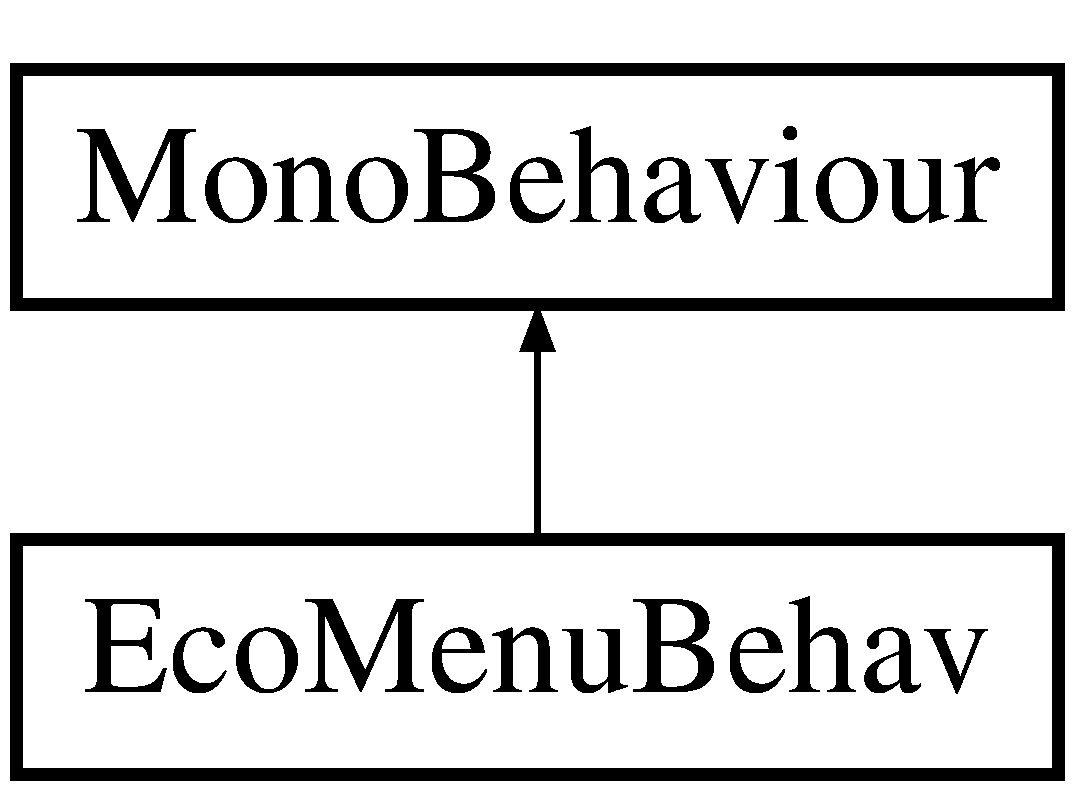
\includegraphics[height=2.000000cm]{class_eco_menu_behav}
\end{center}
\end{figure}
\subsection*{Public Member Functions}
\begin{DoxyCompactItemize}
\item 
void \mbox{\hyperlink{class_eco_menu_behav_a039f9149186291b27affa208529483dc}{load\+Eco\+Menu}} (\mbox{\hyperlink{class_ecosystem}{Ecosystem}} eco)
\begin{DoxyCompactList}\small\item\em creates an ecosystem creator from the provided ecosystem \end{DoxyCompactList}\item 
void \mbox{\hyperlink{class_eco_menu_behav_adbbf966a393af0f1d5893ea17f694dc1}{add\+Creature}} ()
\begin{DoxyCompactList}\small\item\em load the creature editor menu and pass it the current ecosystem editor \end{DoxyCompactList}\item 
void \mbox{\hyperlink{class_eco_menu_behav_a8ea8d6da55e1a0724a33e59ff0b94834}{save\+Settings}} ()
\begin{DoxyCompactList}\small\item\em saves all information that the user entered into the menu \end{DoxyCompactList}\item 
void \mbox{\hyperlink{class_eco_menu_behav_ab08a4156dfbc7df76014ce6dbe6c9577}{add\+Resource}} ()
\end{DoxyCompactItemize}
\subsection*{Public Attributes}
\begin{DoxyCompactItemize}
\item 
Game\+Object \mbox{\hyperlink{class_eco_menu_behav_aa36609d2e9367f75aee215258da4fb65}{u\+I\+Parent}}
\item 
Game\+Object \mbox{\hyperlink{class_eco_menu_behav_a10793ae22e3460867efd47298d5ed492}{error\+Obj}}
\item 
Game\+Object \mbox{\hyperlink{class_eco_menu_behav_a484ff71bd9f8f8ac0e2fa8c91b89a043}{creature\+Menu\+Obj}}
\item 
Game\+Object \mbox{\hyperlink{class_eco_menu_behav_a34b16463f4306afac5cc3371b4b2d401}{lr\+Menu\+Obj}}
\item 
Game\+Object \mbox{\hyperlink{class_eco_menu_behav_ab500173b792e9b3882d2353d8bbf6184}{eco\+Name\+Text\+Box}}
\item 
Game\+Object \mbox{\hyperlink{class_eco_menu_behav_a837b1ff5d43a4fddfacf7c042d832861}{ability\+Pts\+Per\+Creat\+Text\+Box}}
\item 
Game\+Object \mbox{\hyperlink{class_eco_menu_behav_a8568e66599d356a0210a7e255e9e17c7}{comm\+Bits\+Text}}
\item 
Game\+Object \mbox{\hyperlink{class_eco_menu_behav_a7c00751f38f04592adbedc5b325f20fc}{distinct\+Pheno\+Text}}
\item 
Game\+Object \mbox{\hyperlink{class_eco_menu_behav_a369da6c213a6fbd04a4b641418714d59}{time\+Units\+Text}}
\item 
\mbox{\hyperlink{class_ecosystem_editor}{Ecosystem\+Editor}} \mbox{\hyperlink{class_eco_menu_behav_a99428835e845880ae7e65d911a1b9d2a}{eco\+Editor}}
\end{DoxyCompactItemize}


\subsection{Member Function Documentation}
\mbox{\Hypertarget{class_eco_menu_behav_adbbf966a393af0f1d5893ea17f694dc1}\label{class_eco_menu_behav_adbbf966a393af0f1d5893ea17f694dc1}} 
\index{Eco\+Menu\+Behav@{Eco\+Menu\+Behav}!add\+Creature@{add\+Creature}}
\index{add\+Creature@{add\+Creature}!Eco\+Menu\+Behav@{Eco\+Menu\+Behav}}
\subsubsection{\texorpdfstring{add\+Creature()}{addCreature()}}
{\footnotesize\ttfamily void Eco\+Menu\+Behav.\+add\+Creature (\begin{DoxyParamCaption}{ }\end{DoxyParamCaption})}



load the creature editor menu and pass it the current ecosystem editor 

\mbox{\Hypertarget{class_eco_menu_behav_ab08a4156dfbc7df76014ce6dbe6c9577}\label{class_eco_menu_behav_ab08a4156dfbc7df76014ce6dbe6c9577}} 
\index{Eco\+Menu\+Behav@{Eco\+Menu\+Behav}!add\+Resource@{add\+Resource}}
\index{add\+Resource@{add\+Resource}!Eco\+Menu\+Behav@{Eco\+Menu\+Behav}}
\subsubsection{\texorpdfstring{add\+Resource()}{addResource()}}
{\footnotesize\ttfamily void Eco\+Menu\+Behav.\+add\+Resource (\begin{DoxyParamCaption}{ }\end{DoxyParamCaption})}

\mbox{\Hypertarget{class_eco_menu_behav_a039f9149186291b27affa208529483dc}\label{class_eco_menu_behav_a039f9149186291b27affa208529483dc}} 
\index{Eco\+Menu\+Behav@{Eco\+Menu\+Behav}!load\+Eco\+Menu@{load\+Eco\+Menu}}
\index{load\+Eco\+Menu@{load\+Eco\+Menu}!Eco\+Menu\+Behav@{Eco\+Menu\+Behav}}
\subsubsection{\texorpdfstring{load\+Eco\+Menu()}{loadEcoMenu()}}
{\footnotesize\ttfamily void Eco\+Menu\+Behav.\+load\+Eco\+Menu (\begin{DoxyParamCaption}\item[{\mbox{\hyperlink{class_ecosystem}{Ecosystem}}}]{eco }\end{DoxyParamCaption})}



creates an ecosystem creator from the provided ecosystem 

\mbox{\Hypertarget{class_eco_menu_behav_a8ea8d6da55e1a0724a33e59ff0b94834}\label{class_eco_menu_behav_a8ea8d6da55e1a0724a33e59ff0b94834}} 
\index{Eco\+Menu\+Behav@{Eco\+Menu\+Behav}!save\+Settings@{save\+Settings}}
\index{save\+Settings@{save\+Settings}!Eco\+Menu\+Behav@{Eco\+Menu\+Behav}}
\subsubsection{\texorpdfstring{save\+Settings()}{saveSettings()}}
{\footnotesize\ttfamily void Eco\+Menu\+Behav.\+save\+Settings (\begin{DoxyParamCaption}{ }\end{DoxyParamCaption})}



saves all information that the user entered into the menu 

call methods to save eco\+Editor data to actual \mbox{\hyperlink{class_ecosystem}{Ecosystem}} object 

\subsection{Member Data Documentation}
\mbox{\Hypertarget{class_eco_menu_behav_a837b1ff5d43a4fddfacf7c042d832861}\label{class_eco_menu_behav_a837b1ff5d43a4fddfacf7c042d832861}} 
\index{Eco\+Menu\+Behav@{Eco\+Menu\+Behav}!ability\+Pts\+Per\+Creat\+Text\+Box@{ability\+Pts\+Per\+Creat\+Text\+Box}}
\index{ability\+Pts\+Per\+Creat\+Text\+Box@{ability\+Pts\+Per\+Creat\+Text\+Box}!Eco\+Menu\+Behav@{Eco\+Menu\+Behav}}
\subsubsection{\texorpdfstring{ability\+Pts\+Per\+Creat\+Text\+Box}{abilityPtsPerCreatTextBox}}
{\footnotesize\ttfamily Game\+Object Eco\+Menu\+Behav.\+ability\+Pts\+Per\+Creat\+Text\+Box}

\mbox{\Hypertarget{class_eco_menu_behav_a8568e66599d356a0210a7e255e9e17c7}\label{class_eco_menu_behav_a8568e66599d356a0210a7e255e9e17c7}} 
\index{Eco\+Menu\+Behav@{Eco\+Menu\+Behav}!comm\+Bits\+Text@{comm\+Bits\+Text}}
\index{comm\+Bits\+Text@{comm\+Bits\+Text}!Eco\+Menu\+Behav@{Eco\+Menu\+Behav}}
\subsubsection{\texorpdfstring{comm\+Bits\+Text}{commBitsText}}
{\footnotesize\ttfamily Game\+Object Eco\+Menu\+Behav.\+comm\+Bits\+Text}

\mbox{\Hypertarget{class_eco_menu_behav_a484ff71bd9f8f8ac0e2fa8c91b89a043}\label{class_eco_menu_behav_a484ff71bd9f8f8ac0e2fa8c91b89a043}} 
\index{Eco\+Menu\+Behav@{Eco\+Menu\+Behav}!creature\+Menu\+Obj@{creature\+Menu\+Obj}}
\index{creature\+Menu\+Obj@{creature\+Menu\+Obj}!Eco\+Menu\+Behav@{Eco\+Menu\+Behav}}
\subsubsection{\texorpdfstring{creature\+Menu\+Obj}{creatureMenuObj}}
{\footnotesize\ttfamily Game\+Object Eco\+Menu\+Behav.\+creature\+Menu\+Obj}

\mbox{\Hypertarget{class_eco_menu_behav_a7c00751f38f04592adbedc5b325f20fc}\label{class_eco_menu_behav_a7c00751f38f04592adbedc5b325f20fc}} 
\index{Eco\+Menu\+Behav@{Eco\+Menu\+Behav}!distinct\+Pheno\+Text@{distinct\+Pheno\+Text}}
\index{distinct\+Pheno\+Text@{distinct\+Pheno\+Text}!Eco\+Menu\+Behav@{Eco\+Menu\+Behav}}
\subsubsection{\texorpdfstring{distinct\+Pheno\+Text}{distinctPhenoText}}
{\footnotesize\ttfamily Game\+Object Eco\+Menu\+Behav.\+distinct\+Pheno\+Text}

\mbox{\Hypertarget{class_eco_menu_behav_a99428835e845880ae7e65d911a1b9d2a}\label{class_eco_menu_behav_a99428835e845880ae7e65d911a1b9d2a}} 
\index{Eco\+Menu\+Behav@{Eco\+Menu\+Behav}!eco\+Editor@{eco\+Editor}}
\index{eco\+Editor@{eco\+Editor}!Eco\+Menu\+Behav@{Eco\+Menu\+Behav}}
\subsubsection{\texorpdfstring{eco\+Editor}{ecoEditor}}
{\footnotesize\ttfamily \mbox{\hyperlink{class_ecosystem_editor}{Ecosystem\+Editor}} Eco\+Menu\+Behav.\+eco\+Editor}

\mbox{\Hypertarget{class_eco_menu_behav_ab500173b792e9b3882d2353d8bbf6184}\label{class_eco_menu_behav_ab500173b792e9b3882d2353d8bbf6184}} 
\index{Eco\+Menu\+Behav@{Eco\+Menu\+Behav}!eco\+Name\+Text\+Box@{eco\+Name\+Text\+Box}}
\index{eco\+Name\+Text\+Box@{eco\+Name\+Text\+Box}!Eco\+Menu\+Behav@{Eco\+Menu\+Behav}}
\subsubsection{\texorpdfstring{eco\+Name\+Text\+Box}{ecoNameTextBox}}
{\footnotesize\ttfamily Game\+Object Eco\+Menu\+Behav.\+eco\+Name\+Text\+Box}

\mbox{\Hypertarget{class_eco_menu_behav_a10793ae22e3460867efd47298d5ed492}\label{class_eco_menu_behav_a10793ae22e3460867efd47298d5ed492}} 
\index{Eco\+Menu\+Behav@{Eco\+Menu\+Behav}!error\+Obj@{error\+Obj}}
\index{error\+Obj@{error\+Obj}!Eco\+Menu\+Behav@{Eco\+Menu\+Behav}}
\subsubsection{\texorpdfstring{error\+Obj}{errorObj}}
{\footnotesize\ttfamily Game\+Object Eco\+Menu\+Behav.\+error\+Obj}

\mbox{\Hypertarget{class_eco_menu_behav_a34b16463f4306afac5cc3371b4b2d401}\label{class_eco_menu_behav_a34b16463f4306afac5cc3371b4b2d401}} 
\index{Eco\+Menu\+Behav@{Eco\+Menu\+Behav}!lr\+Menu\+Obj@{lr\+Menu\+Obj}}
\index{lr\+Menu\+Obj@{lr\+Menu\+Obj}!Eco\+Menu\+Behav@{Eco\+Menu\+Behav}}
\subsubsection{\texorpdfstring{lr\+Menu\+Obj}{lrMenuObj}}
{\footnotesize\ttfamily Game\+Object Eco\+Menu\+Behav.\+lr\+Menu\+Obj}

\mbox{\Hypertarget{class_eco_menu_behav_a369da6c213a6fbd04a4b641418714d59}\label{class_eco_menu_behav_a369da6c213a6fbd04a4b641418714d59}} 
\index{Eco\+Menu\+Behav@{Eco\+Menu\+Behav}!time\+Units\+Text@{time\+Units\+Text}}
\index{time\+Units\+Text@{time\+Units\+Text}!Eco\+Menu\+Behav@{Eco\+Menu\+Behav}}
\subsubsection{\texorpdfstring{time\+Units\+Text}{timeUnitsText}}
{\footnotesize\ttfamily Game\+Object Eco\+Menu\+Behav.\+time\+Units\+Text}

\mbox{\Hypertarget{class_eco_menu_behav_aa36609d2e9367f75aee215258da4fb65}\label{class_eco_menu_behav_aa36609d2e9367f75aee215258da4fb65}} 
\index{Eco\+Menu\+Behav@{Eco\+Menu\+Behav}!u\+I\+Parent@{u\+I\+Parent}}
\index{u\+I\+Parent@{u\+I\+Parent}!Eco\+Menu\+Behav@{Eco\+Menu\+Behav}}
\subsubsection{\texorpdfstring{u\+I\+Parent}{uIParent}}
{\footnotesize\ttfamily Game\+Object Eco\+Menu\+Behav.\+u\+I\+Parent}



The documentation for this class was generated from the following file\+:\begin{DoxyCompactItemize}
\item 
\mbox{\hyperlink{_eco_menu_behav_8cs}{Eco\+Menu\+Behav.\+cs}}\end{DoxyCompactItemize}

\hypertarget{class_eco_menu_tester}{}\section{Eco\+Menu\+Tester Class Reference}
\label{class_eco_menu_tester}\index{Eco\+Menu\+Tester@{Eco\+Menu\+Tester}}
Inheritance diagram for Eco\+Menu\+Tester\+:\begin{figure}[H]
\begin{center}
\leavevmode
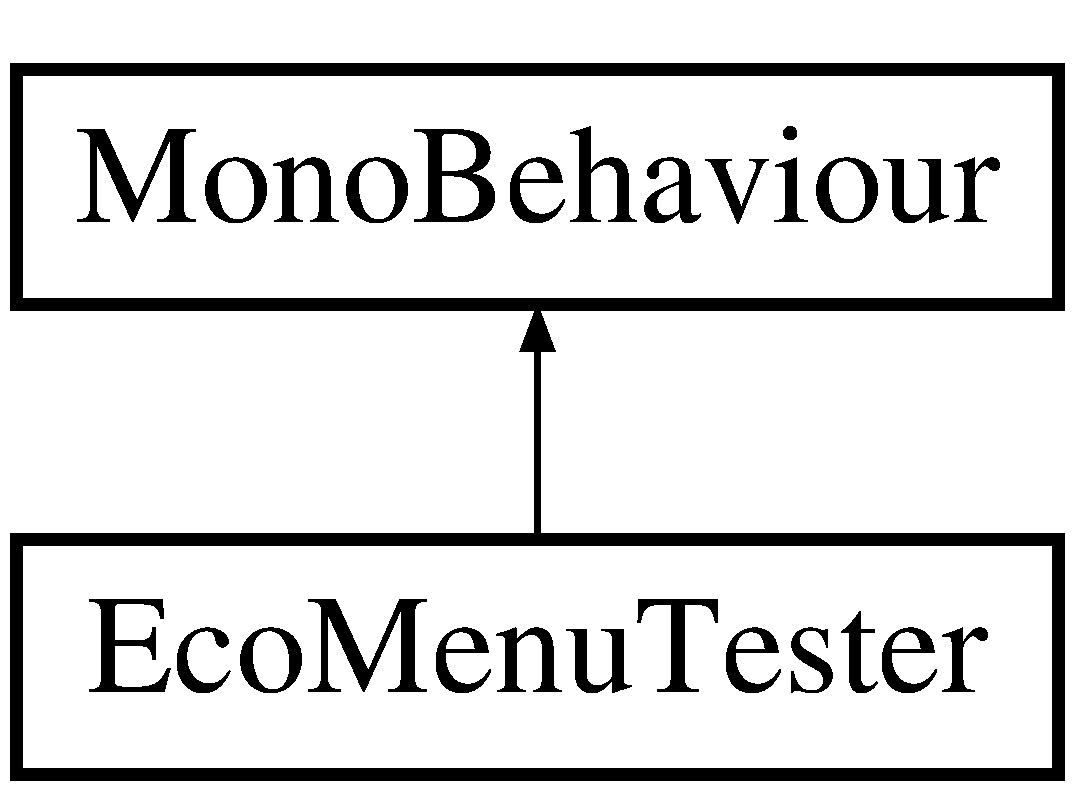
\includegraphics[height=2.000000cm]{class_eco_menu_tester}
\end{center}
\end{figure}


The documentation for this class was generated from the following file\+:\begin{DoxyCompactItemize}
\item 
\mbox{\hyperlink{_eco_menu_tester_8cs}{Eco\+Menu\+Tester.\+cs}}\end{DoxyCompactItemize}

\hypertarget{class_ecosystem}{}\section{Ecosystem Class Reference}
\label{class_ecosystem}\index{Ecosystem@{Ecosystem}}


This class contains all of the data about the state of the ecosystem including the populations, species templates, map, resources, and other general parameters.  


\subsection*{Public Member Functions}
\begin{DoxyCompactItemize}
\item 
void \mbox{\hyperlink{class_ecosystem_a2102d1d4f820c9913cccaf917df9879f}{run\+System}} (int time\+Steps)
\begin{DoxyCompactList}\small\item\em run ecosystem for a certain number of time steps \end{DoxyCompactList}\item 
void \mbox{\hyperlink{class_ecosystem_a3d2b11c7fe8b6699eee72fc77fa02d1d}{add\+Species}} (\mbox{\hyperlink{class_creature}{Creature}} creature)
\begin{DoxyCompactList}\small\item\em creates new species in dictionary based on given creature \end{DoxyCompactList}\item 
void \mbox{\hyperlink{class_ecosystem_a887af939d4bf8e17701dc1a4af875e7f}{create\+Population}} (int size, \mbox{\hyperlink{class_creature}{Creature}} \mbox{\hyperlink{class_ecosystem_a3cd0f83955fce1623326b58666a6a9af}{species}})
\item 
\mbox{\hyperlink{class_ecosystem}{Ecosystem}} \mbox{\hyperlink{class_ecosystem_a0e082a9b5c6e6df9cbe20da26d1d6968}{shallow\+Copy}} ()
\item 
void \mbox{\hyperlink{class_ecosystem_a24d493832618dbfccb61812635c2fbdf}{update\+Texture}} ()
\end{DoxyCompactItemize}
\subsection*{Public Attributes}
\begin{DoxyCompactItemize}
\item 
string \mbox{\hyperlink{class_ecosystem_ae22d1e48d43e1818705c5eda52785f63}{name}} = \char`\"{}default\char`\"{}
\item 
Dictionary$<$ string, \mbox{\hyperlink{class_population}{Population}} $>$ \mbox{\hyperlink{class_ecosystem_a8b17a9aebf9aa2619901cd3fe96c8d66}{populations}} = new Dictionary$<$string, \mbox{\hyperlink{class_population}{Population}}$>$()
\begin{DoxyCompactList}\small\item\em Lists of creatures, organized by species name in dictionary. \end{DoxyCompactList}\item 
List$<$ List$<$ \mbox{\hyperlink{class_land}{Land}} $>$ $>$ \mbox{\hyperlink{class_ecosystem_a03ba5f09ddfade51a644ec7f47349607}{map}} = new List$<$List$<$\mbox{\hyperlink{class_land}{Land}}$>$$>$()
\begin{DoxyCompactList}\small\item\em map of land spaces \end{DoxyCompactList}\item 
int \mbox{\hyperlink{class_ecosystem_a3aa718428180c38f22774b736fb4b9d3}{length}}
\begin{DoxyCompactList}\small\item\em Length of map \end{DoxyCompactList}\item 
int \mbox{\hyperlink{class_ecosystem_acd13711fb3bdc5aafb4d70ccd069d385}{width}}
\begin{DoxyCompactList}\small\item\em Width of map \end{DoxyCompactList}\item 
int \mbox{\hyperlink{class_ecosystem_a7371b349e3dcf7f22a0ab2cab61e48c8}{comm\+Bits}}
\item 
Dictionary$<$ string, \mbox{\hyperlink{class_creature}{Creature}} $>$ \mbox{\hyperlink{class_ecosystem_a3cd0f83955fce1623326b58666a6a9af}{species}} = new Dictionary$<$string, \mbox{\hyperlink{class_creature}{Creature}}$>$()
\begin{DoxyCompactList}\small\item\em Pool of species (proto-\/creatures) that can be used to generate new populations. \end{DoxyCompactList}\item 
int \mbox{\hyperlink{class_ecosystem_a7347a85ab0ac674a837ceefa63a3173c}{distict\+Phenotypes}}
\begin{DoxyCompactList}\small\item\em Number of possible phenotypes a creature can take on. \end{DoxyCompactList}\item 
int \mbox{\hyperlink{class_ecosystem_af1e2bcc0bc7096df0c326953813ca94d}{ability\+Points\+Per\+Creature}}
\begin{DoxyCompactList}\small\item\em Max number of ability points that each creature has to assign. \end{DoxyCompactList}\item 
Dictionary$<$ string, \mbox{\hyperlink{class_resource_store}{Resource\+Store}} $>$ \mbox{\hyperlink{class_ecosystem_adf42dce1cde9124f1ffb5b729967fc1a}{resource\+Options}} = new Dictionary$<$string, \mbox{\hyperlink{class_resource_store}{Resource\+Store}}$>$()
\begin{DoxyCompactList}\small\item\em List of resources that can be stored on Lands. \end{DoxyCompactList}\item 
float \mbox{\hyperlink{class_ecosystem_a4eb1b47f3b158dc533ad6c2983b2f481}{time\+Units\+Per\+Turn}}
\item 
int \mbox{\hyperlink{class_ecosystem_aad967a97d8bc9886ad764bdb3c85a83a}{age}} = 0
\item 
int \mbox{\hyperlink{class_ecosystem_a6856c0300199a5acee23d631f18f4a46}{renew\+Interval\+Steps}} = 10
\item 
Color \mbox{[}$\,$\mbox{]} \mbox{\hyperlink{class_ecosystem_ac2539557244002ab323da79ca480e281}{colors}}
\end{DoxyCompactItemize}


\subsection{Detailed Description}
This class contains all of the data about the state of the ecosystem including the populations, species templates, map, resources, and other general parameters. 



\subsection{Member Function Documentation}
\mbox{\Hypertarget{class_ecosystem_a3d2b11c7fe8b6699eee72fc77fa02d1d}\label{class_ecosystem_a3d2b11c7fe8b6699eee72fc77fa02d1d}} 
\index{Ecosystem@{Ecosystem}!add\+Species@{add\+Species}}
\index{add\+Species@{add\+Species}!Ecosystem@{Ecosystem}}
\subsubsection{\texorpdfstring{add\+Species()}{addSpecies()}}
{\footnotesize\ttfamily void Ecosystem.\+add\+Species (\begin{DoxyParamCaption}\item[{\mbox{\hyperlink{class_creature}{Creature}}}]{creature }\end{DoxyParamCaption})}



creates new species in dictionary based on given creature 

\mbox{\Hypertarget{class_ecosystem_a887af939d4bf8e17701dc1a4af875e7f}\label{class_ecosystem_a887af939d4bf8e17701dc1a4af875e7f}} 
\index{Ecosystem@{Ecosystem}!create\+Population@{create\+Population}}
\index{create\+Population@{create\+Population}!Ecosystem@{Ecosystem}}
\subsubsection{\texorpdfstring{create\+Population()}{createPopulation()}}
{\footnotesize\ttfamily void Ecosystem.\+create\+Population (\begin{DoxyParamCaption}\item[{int}]{size,  }\item[{\mbox{\hyperlink{class_creature}{Creature}}}]{species }\end{DoxyParamCaption})}

\mbox{\Hypertarget{class_ecosystem_a2102d1d4f820c9913cccaf917df9879f}\label{class_ecosystem_a2102d1d4f820c9913cccaf917df9879f}} 
\index{Ecosystem@{Ecosystem}!run\+System@{run\+System}}
\index{run\+System@{run\+System}!Ecosystem@{Ecosystem}}
\subsubsection{\texorpdfstring{run\+System()}{runSystem()}}
{\footnotesize\ttfamily void Ecosystem.\+run\+System (\begin{DoxyParamCaption}\item[{int}]{time\+Steps }\end{DoxyParamCaption})}



run ecosystem for a certain number of time steps 

\mbox{\Hypertarget{class_ecosystem_a0e082a9b5c6e6df9cbe20da26d1d6968}\label{class_ecosystem_a0e082a9b5c6e6df9cbe20da26d1d6968}} 
\index{Ecosystem@{Ecosystem}!shallow\+Copy@{shallow\+Copy}}
\index{shallow\+Copy@{shallow\+Copy}!Ecosystem@{Ecosystem}}
\subsubsection{\texorpdfstring{shallow\+Copy()}{shallowCopy()}}
{\footnotesize\ttfamily \mbox{\hyperlink{class_ecosystem}{Ecosystem}} Ecosystem.\+shallow\+Copy (\begin{DoxyParamCaption}{ }\end{DoxyParamCaption})}

\mbox{\Hypertarget{class_ecosystem_a24d493832618dbfccb61812635c2fbdf}\label{class_ecosystem_a24d493832618dbfccb61812635c2fbdf}} 
\index{Ecosystem@{Ecosystem}!update\+Texture@{update\+Texture}}
\index{update\+Texture@{update\+Texture}!Ecosystem@{Ecosystem}}
\subsubsection{\texorpdfstring{update\+Texture()}{updateTexture()}}
{\footnotesize\ttfamily void Ecosystem.\+update\+Texture (\begin{DoxyParamCaption}{ }\end{DoxyParamCaption})}

Texture stuff below 

\subsection{Member Data Documentation}
\mbox{\Hypertarget{class_ecosystem_af1e2bcc0bc7096df0c326953813ca94d}\label{class_ecosystem_af1e2bcc0bc7096df0c326953813ca94d}} 
\index{Ecosystem@{Ecosystem}!ability\+Points\+Per\+Creature@{ability\+Points\+Per\+Creature}}
\index{ability\+Points\+Per\+Creature@{ability\+Points\+Per\+Creature}!Ecosystem@{Ecosystem}}
\subsubsection{\texorpdfstring{ability\+Points\+Per\+Creature}{abilityPointsPerCreature}}
{\footnotesize\ttfamily int Ecosystem.\+ability\+Points\+Per\+Creature}



Max number of ability points that each creature has to assign. 

\mbox{\Hypertarget{class_ecosystem_aad967a97d8bc9886ad764bdb3c85a83a}\label{class_ecosystem_aad967a97d8bc9886ad764bdb3c85a83a}} 
\index{Ecosystem@{Ecosystem}!age@{age}}
\index{age@{age}!Ecosystem@{Ecosystem}}
\subsubsection{\texorpdfstring{age}{age}}
{\footnotesize\ttfamily int Ecosystem.\+age = 0}

\mbox{\Hypertarget{class_ecosystem_ac2539557244002ab323da79ca480e281}\label{class_ecosystem_ac2539557244002ab323da79ca480e281}} 
\index{Ecosystem@{Ecosystem}!colors@{colors}}
\index{colors@{colors}!Ecosystem@{Ecosystem}}
\subsubsection{\texorpdfstring{colors}{colors}}
{\footnotesize\ttfamily Color \mbox{[}$\,$\mbox{]} Ecosystem.\+colors}

\mbox{\Hypertarget{class_ecosystem_a7371b349e3dcf7f22a0ab2cab61e48c8}\label{class_ecosystem_a7371b349e3dcf7f22a0ab2cab61e48c8}} 
\index{Ecosystem@{Ecosystem}!comm\+Bits@{comm\+Bits}}
\index{comm\+Bits@{comm\+Bits}!Ecosystem@{Ecosystem}}
\subsubsection{\texorpdfstring{comm\+Bits}{commBits}}
{\footnotesize\ttfamily int Ecosystem.\+comm\+Bits}

\mbox{\Hypertarget{class_ecosystem_a7347a85ab0ac674a837ceefa63a3173c}\label{class_ecosystem_a7347a85ab0ac674a837ceefa63a3173c}} 
\index{Ecosystem@{Ecosystem}!distict\+Phenotypes@{distict\+Phenotypes}}
\index{distict\+Phenotypes@{distict\+Phenotypes}!Ecosystem@{Ecosystem}}
\subsubsection{\texorpdfstring{distict\+Phenotypes}{distictPhenotypes}}
{\footnotesize\ttfamily int Ecosystem.\+distict\+Phenotypes}



Number of possible phenotypes a creature can take on. 

\mbox{\Hypertarget{class_ecosystem_a3aa718428180c38f22774b736fb4b9d3}\label{class_ecosystem_a3aa718428180c38f22774b736fb4b9d3}} 
\index{Ecosystem@{Ecosystem}!length@{length}}
\index{length@{length}!Ecosystem@{Ecosystem}}
\subsubsection{\texorpdfstring{length}{length}}
{\footnotesize\ttfamily int Ecosystem.\+length}



Length of map 

\mbox{\Hypertarget{class_ecosystem_a03ba5f09ddfade51a644ec7f47349607}\label{class_ecosystem_a03ba5f09ddfade51a644ec7f47349607}} 
\index{Ecosystem@{Ecosystem}!map@{map}}
\index{map@{map}!Ecosystem@{Ecosystem}}
\subsubsection{\texorpdfstring{map}{map}}
{\footnotesize\ttfamily List$<$List$<$\mbox{\hyperlink{class_land}{Land}}$>$ $>$ Ecosystem.\+map = new List$<$List$<$\mbox{\hyperlink{class_land}{Land}}$>$$>$()}



map of land spaces 

\mbox{\Hypertarget{class_ecosystem_ae22d1e48d43e1818705c5eda52785f63}\label{class_ecosystem_ae22d1e48d43e1818705c5eda52785f63}} 
\index{Ecosystem@{Ecosystem}!name@{name}}
\index{name@{name}!Ecosystem@{Ecosystem}}
\subsubsection{\texorpdfstring{name}{name}}
{\footnotesize\ttfamily string Ecosystem.\+name = \char`\"{}default\char`\"{}}

\mbox{\Hypertarget{class_ecosystem_a8b17a9aebf9aa2619901cd3fe96c8d66}\label{class_ecosystem_a8b17a9aebf9aa2619901cd3fe96c8d66}} 
\index{Ecosystem@{Ecosystem}!populations@{populations}}
\index{populations@{populations}!Ecosystem@{Ecosystem}}
\subsubsection{\texorpdfstring{populations}{populations}}
{\footnotesize\ttfamily Dictionary$<$string, \mbox{\hyperlink{class_population}{Population}}$>$ Ecosystem.\+populations = new Dictionary$<$string, \mbox{\hyperlink{class_population}{Population}}$>$()}



Lists of creatures, organized by species name in dictionary. 

\mbox{\Hypertarget{class_ecosystem_a6856c0300199a5acee23d631f18f4a46}\label{class_ecosystem_a6856c0300199a5acee23d631f18f4a46}} 
\index{Ecosystem@{Ecosystem}!renew\+Interval\+Steps@{renew\+Interval\+Steps}}
\index{renew\+Interval\+Steps@{renew\+Interval\+Steps}!Ecosystem@{Ecosystem}}
\subsubsection{\texorpdfstring{renew\+Interval\+Steps}{renewIntervalSteps}}
{\footnotesize\ttfamily int Ecosystem.\+renew\+Interval\+Steps = 10}

\mbox{\Hypertarget{class_ecosystem_adf42dce1cde9124f1ffb5b729967fc1a}\label{class_ecosystem_adf42dce1cde9124f1ffb5b729967fc1a}} 
\index{Ecosystem@{Ecosystem}!resource\+Options@{resource\+Options}}
\index{resource\+Options@{resource\+Options}!Ecosystem@{Ecosystem}}
\subsubsection{\texorpdfstring{resource\+Options}{resourceOptions}}
{\footnotesize\ttfamily Dictionary$<$string, \mbox{\hyperlink{class_resource_store}{Resource\+Store}}$>$ Ecosystem.\+resource\+Options = new Dictionary$<$string, \mbox{\hyperlink{class_resource_store}{Resource\+Store}}$>$()}



List of resources that can be stored on Lands. 

\mbox{\Hypertarget{class_ecosystem_a3cd0f83955fce1623326b58666a6a9af}\label{class_ecosystem_a3cd0f83955fce1623326b58666a6a9af}} 
\index{Ecosystem@{Ecosystem}!species@{species}}
\index{species@{species}!Ecosystem@{Ecosystem}}
\subsubsection{\texorpdfstring{species}{species}}
{\footnotesize\ttfamily Dictionary$<$string, \mbox{\hyperlink{class_creature}{Creature}}$>$ Ecosystem.\+species = new Dictionary$<$string, \mbox{\hyperlink{class_creature}{Creature}}$>$()}



Pool of species (proto-\/creatures) that can be used to generate new populations. 

\mbox{\Hypertarget{class_ecosystem_a4eb1b47f3b158dc533ad6c2983b2f481}\label{class_ecosystem_a4eb1b47f3b158dc533ad6c2983b2f481}} 
\index{Ecosystem@{Ecosystem}!time\+Units\+Per\+Turn@{time\+Units\+Per\+Turn}}
\index{time\+Units\+Per\+Turn@{time\+Units\+Per\+Turn}!Ecosystem@{Ecosystem}}
\subsubsection{\texorpdfstring{time\+Units\+Per\+Turn}{timeUnitsPerTurn}}
{\footnotesize\ttfamily float Ecosystem.\+time\+Units\+Per\+Turn}

\mbox{\Hypertarget{class_ecosystem_acd13711fb3bdc5aafb4d70ccd069d385}\label{class_ecosystem_acd13711fb3bdc5aafb4d70ccd069d385}} 
\index{Ecosystem@{Ecosystem}!width@{width}}
\index{width@{width}!Ecosystem@{Ecosystem}}
\subsubsection{\texorpdfstring{width}{width}}
{\footnotesize\ttfamily int Ecosystem.\+width}



Width of map 



The documentation for this class was generated from the following file\+:\begin{DoxyCompactItemize}
\item 
\mbox{\hyperlink{_ecosystem_8cs}{Ecosystem.\+cs}}\end{DoxyCompactItemize}

\hypertarget{class_ecosystem_editor}{}\section{Ecosystem\+Editor Class Reference}
\label{class_ecosystem_editor}\index{Ecosystem\+Editor@{Ecosystem\+Editor}}


A\+PI for alterning ecosystem.  


\subsection*{Public Member Functions}
\begin{DoxyCompactItemize}
\item 
\mbox{\hyperlink{class_ecosystem_editor_ae398c2a58464b4f994929f22c71c36cc}{Ecosystem\+Editor}} (\mbox{\hyperlink{class_ecosystem}{Ecosystem}} \+\_\+ecosystem)
\item 
void \mbox{\hyperlink{class_ecosystem_editor_a9ac3559972dcc89445df6a6817c938f0}{set\+Ability\+Points\+Per\+Creature}} (int ability\+Points)
\item 
void \mbox{\hyperlink{class_ecosystem_editor_a079f04c589520a420be5c749dcb81447}{set\+Comm\+Bits}} (int num\+Bits)
\item 
void \mbox{\hyperlink{class_ecosystem_editor_a11d1e048c710c397a3cde9354d4117c3}{set\+Distinct\+Phenotype\+Num}} (int num\+Phenotypes)
\item 
void \mbox{\hyperlink{class_ecosystem_editor_a5012174c9ae01075e7749739f2700f69}{set\+Time\+Units\+Per\+Turn}} (int time\+Units)
\item 
void \mbox{\hyperlink{class_ecosystem_editor_a809bdfc28dc15c7cdbb2bde538bd34e9}{set\+Name}} (string name)
\begin{DoxyCompactList}\small\item\em sets name of dictionary to use when loading \end{DoxyCompactList}\item 
void \mbox{\hyperlink{class_ecosystem_editor_a9ba5901625731091af68a400689a2c44}{set\+Renew\+Interval}} (int renew\+Steps)
\begin{DoxyCompactList}\small\item\em sets number of steps between each renewal of resources. \end{DoxyCompactList}\item 
\mbox{\hyperlink{class_land_resource_editor}{Land\+Resource\+Editor}} \mbox{\hyperlink{class_ecosystem_editor_a8473ee588e7e2201b6c57bd7204ec803}{add\+Resource}} (string resource\+Name)
\begin{DoxyCompactList}\small\item\em 
\begin{DoxyParams}{Parameters}
{\em resource\+Name} & Name of resource\+: used as key in dictionary.\\
\hline
\end{DoxyParams}
\end{DoxyCompactList}\item 
\mbox{\hyperlink{class_creature_editor}{Creature\+Editor}} \mbox{\hyperlink{class_ecosystem_editor_a818800b8e8a812dd061e85a8f2a483b7}{add\+Creature}} ()
\begin{DoxyCompactList}\small\item\em \mbox{\hyperlink{class_creature}{Creature}} new creature \end{DoxyCompactList}\item 
\mbox{\hyperlink{class_species_populator}{Species\+Populator}} \mbox{\hyperlink{class_ecosystem_editor_a3f0623c56b5399b02f6b18a72652a1ba}{populate\+Species}} (string founder\+Species)
\item 
\mbox{\hyperlink{class_map_editor}{Map\+Editor}} \mbox{\hyperlink{class_ecosystem_editor_a34ac5bdf72932adfbdf5758a8f42a836}{create\+Map}} ()
\item 
void \mbox{\hyperlink{class_ecosystem_editor_a1d369adb1216181a3db5cdde1baf50af}{save\+Resource}} ()
\begin{DoxyCompactList}\small\item\em Saves a newly created resource to resource\+Options. \end{DoxyCompactList}\item 
void \mbox{\hyperlink{class_ecosystem_editor_af57a50510d4baf7cc372fc2b32c38ead}{save\+Resource\+Options}} ()
\begin{DoxyCompactList}\small\item\em Saves created resource\+Options to ecosystems actual resource options. \end{DoxyCompactList}\item 
void \mbox{\hyperlink{class_ecosystem_editor_a22b8b780750a21d6b893e417f623ba30}{add\+To\+Founders}} ()
\item 
void \mbox{\hyperlink{class_ecosystem_editor_a5aa46063ae1157099b036e81cdcbe2ad}{save\+Founders\+To\+Species}} ()
\begin{DoxyCompactList}\small\item\em Saves founders to ecosystem\textquotesingle{}s species dictionary. \end{DoxyCompactList}\item 
void \mbox{\hyperlink{class_ecosystem_editor_a5df7d2d657419e3a35f2b55973f7c6ef}{save\+Current\+Population}} ()
\begin{DoxyCompactList}\small\item\em Saves population creatured by species\+Populator to current\+Population. \end{DoxyCompactList}\item 
void \mbox{\hyperlink{class_ecosystem_editor_a561f235d70f14111eba609e5d5ea869b}{save\+Edited\+Map}} ()
\item 
void \mbox{\hyperlink{class_ecosystem_editor_acfbb3166d4c0ef8567a36cf66b456141}{save\+Map}} ()
\begin{DoxyCompactList}\small\item\em Saves tentative map to actual ecosystem map. \end{DoxyCompactList}\item 
void \mbox{\hyperlink{class_ecosystem_editor_a8a9917b9c31e71e610d9e4b231930ce3}{add\+Current\+Population\+To\+Ecosystem}} ()
\begin{DoxyCompactList}\small\item\em Saves current\+Population to ecosystem.\+populations \end{DoxyCompactList}\item 
void \mbox{\hyperlink{class_ecosystem_editor_af6f631b9a71a8e1f7de9d48d18ddd08a}{add\+Current\+Population\+To\+Map}} ()
\begin{DoxyCompactList}\small\item\em adds a population to the tentative map. \end{DoxyCompactList}\end{DoxyCompactItemize}
\subsection*{Public Attributes}
\begin{DoxyCompactItemize}
\item 
\mbox{\hyperlink{class_ecosystem}{Ecosystem}} \mbox{\hyperlink{class_ecosystem_editor_a49e0702cf9757efdf05a098336737890}{ecosystem}}
\begin{DoxyCompactList}\small\item\em \mbox{\hyperlink{class_ecosystem}{Ecosystem}} to be created. \end{DoxyCompactList}\item 
\mbox{\hyperlink{class_land_resource_editor}{Land\+Resource\+Editor}} \mbox{\hyperlink{class_ecosystem_editor_a1879450c7d71911c3a0f5b12cc287b2b}{lre}}
\begin{DoxyCompactList}\small\item\em Creates Lands to add to Eco\+System resource\+Options. \end{DoxyCompactList}\item 
\mbox{\hyperlink{class_map_editor}{Map\+Editor}} \mbox{\hyperlink{class_ecosystem_editor_ae2dd3be1675ac49fe39d706cef093386}{map\+Editor}}
\begin{DoxyCompactList}\small\item\em Edits map of lands. \end{DoxyCompactList}\item 
\mbox{\hyperlink{class_creature_editor}{Creature\+Editor}} \mbox{\hyperlink{class_ecosystem_editor_ae07c75810b8d9ff769bf1cd552786138}{creature\+Creator}}
\begin{DoxyCompactList}\small\item\em For generating founder creatures. \end{DoxyCompactList}\item 
Dictionary$<$ string, \mbox{\hyperlink{class_creature}{Creature}} $>$ \mbox{\hyperlink{class_ecosystem_editor_a3b9c67b19a314455f9eaf3eaa0cbe341}{founder\+Creatures}}
\begin{DoxyCompactList}\small\item\em Creatures used to generate populations. \end{DoxyCompactList}\item 
\mbox{\hyperlink{class_species_populator}{Species\+Populator}} \mbox{\hyperlink{class_ecosystem_editor_abe484ddd93b48d1300e88ab531d56aec}{species\+Populator}}
\begin{DoxyCompactList}\small\item\em Users founder and map to populate species. \end{DoxyCompactList}\item 
Dictionary$<$ string, List$<$ \mbox{\hyperlink{class_creature}{Creature}} $>$ $>$ \mbox{\hyperlink{class_ecosystem_editor_abea7f35b0d4980aad82dac92b6011993}{populations}} = new Dictionary$<$string, List$<$\mbox{\hyperlink{class_creature}{Creature}}$>$$>$()
\begin{DoxyCompactList}\small\item\em Stores populations of creatures. \end{DoxyCompactList}\item 
Dictionary$<$ string, \mbox{\hyperlink{class_resource_store}{Resource\+Store}} $>$ \mbox{\hyperlink{class_ecosystem_editor_aa0e6ad8b42512f087178aca21464da02}{tentative\+Resource\+Options}}
\begin{DoxyCompactList}\small\item\em Tenative list of resource options. \end{DoxyCompactList}\item 
List$<$ List$<$ \mbox{\hyperlink{class_land}{Land}} $>$ $>$ \mbox{\hyperlink{class_ecosystem_editor_a40077803f584d6c42951feac3569a972}{tentative\+Map}} = new List$<$List$<$\mbox{\hyperlink{class_land}{Land}}$>$$>$()
\begin{DoxyCompactList}\small\item\em Tentative map to be saved to ecosystem map when save\+Map is called. \end{DoxyCompactList}\end{DoxyCompactItemize}


\subsection{Detailed Description}
A\+PI for alterning ecosystem. 



\subsection{Constructor \& Destructor Documentation}
\mbox{\Hypertarget{class_ecosystem_editor_ae398c2a58464b4f994929f22c71c36cc}\label{class_ecosystem_editor_ae398c2a58464b4f994929f22c71c36cc}} 
\index{Ecosystem\+Editor@{Ecosystem\+Editor}!Ecosystem\+Editor@{Ecosystem\+Editor}}
\index{Ecosystem\+Editor@{Ecosystem\+Editor}!Ecosystem\+Editor@{Ecosystem\+Editor}}
\subsubsection{\texorpdfstring{Ecosystem\+Editor()}{EcosystemEditor()}}
{\footnotesize\ttfamily Ecosystem\+Editor.\+Ecosystem\+Editor (\begin{DoxyParamCaption}\item[{\mbox{\hyperlink{class_ecosystem}{Ecosystem}}}]{\+\_\+ecosystem }\end{DoxyParamCaption})}



\subsection{Member Function Documentation}
\mbox{\Hypertarget{class_ecosystem_editor_a818800b8e8a812dd061e85a8f2a483b7}\label{class_ecosystem_editor_a818800b8e8a812dd061e85a8f2a483b7}} 
\index{Ecosystem\+Editor@{Ecosystem\+Editor}!add\+Creature@{add\+Creature}}
\index{add\+Creature@{add\+Creature}!Ecosystem\+Editor@{Ecosystem\+Editor}}
\subsubsection{\texorpdfstring{add\+Creature()}{addCreature()}}
{\footnotesize\ttfamily \mbox{\hyperlink{class_creature_editor}{Creature\+Editor}} Ecosystem\+Editor.\+add\+Creature (\begin{DoxyParamCaption}{ }\end{DoxyParamCaption})}



\mbox{\hyperlink{class_creature}{Creature}} new creature 

\mbox{\Hypertarget{class_ecosystem_editor_a8a9917b9c31e71e610d9e4b231930ce3}\label{class_ecosystem_editor_a8a9917b9c31e71e610d9e4b231930ce3}} 
\index{Ecosystem\+Editor@{Ecosystem\+Editor}!add\+Current\+Population\+To\+Ecosystem@{add\+Current\+Population\+To\+Ecosystem}}
\index{add\+Current\+Population\+To\+Ecosystem@{add\+Current\+Population\+To\+Ecosystem}!Ecosystem\+Editor@{Ecosystem\+Editor}}
\subsubsection{\texorpdfstring{add\+Current\+Population\+To\+Ecosystem()}{addCurrentPopulationToEcosystem()}}
{\footnotesize\ttfamily void Ecosystem\+Editor.\+add\+Current\+Population\+To\+Ecosystem (\begin{DoxyParamCaption}{ }\end{DoxyParamCaption})}



Saves current\+Population to ecosystem.\+populations 

\mbox{\Hypertarget{class_ecosystem_editor_af6f631b9a71a8e1f7de9d48d18ddd08a}\label{class_ecosystem_editor_af6f631b9a71a8e1f7de9d48d18ddd08a}} 
\index{Ecosystem\+Editor@{Ecosystem\+Editor}!add\+Current\+Population\+To\+Map@{add\+Current\+Population\+To\+Map}}
\index{add\+Current\+Population\+To\+Map@{add\+Current\+Population\+To\+Map}!Ecosystem\+Editor@{Ecosystem\+Editor}}
\subsubsection{\texorpdfstring{add\+Current\+Population\+To\+Map()}{addCurrentPopulationToMap()}}
{\footnotesize\ttfamily void Ecosystem\+Editor.\+add\+Current\+Population\+To\+Map (\begin{DoxyParamCaption}{ }\end{DoxyParamCaption})}



adds a population to the tentative map. 

\mbox{\Hypertarget{class_ecosystem_editor_a8473ee588e7e2201b6c57bd7204ec803}\label{class_ecosystem_editor_a8473ee588e7e2201b6c57bd7204ec803}} 
\index{Ecosystem\+Editor@{Ecosystem\+Editor}!add\+Resource@{add\+Resource}}
\index{add\+Resource@{add\+Resource}!Ecosystem\+Editor@{Ecosystem\+Editor}}
\subsubsection{\texorpdfstring{add\+Resource()}{addResource()}}
{\footnotesize\ttfamily \mbox{\hyperlink{class_land_resource_editor}{Land\+Resource\+Editor}} Ecosystem\+Editor.\+add\+Resource (\begin{DoxyParamCaption}\item[{string}]{resource\+Name }\end{DoxyParamCaption})}




\begin{DoxyParams}{Parameters}
{\em resource\+Name} & Name of resource\+: used as key in dictionary.\\
\hline
\end{DoxyParams}


\mbox{\Hypertarget{class_ecosystem_editor_a22b8b780750a21d6b893e417f623ba30}\label{class_ecosystem_editor_a22b8b780750a21d6b893e417f623ba30}} 
\index{Ecosystem\+Editor@{Ecosystem\+Editor}!add\+To\+Founders@{add\+To\+Founders}}
\index{add\+To\+Founders@{add\+To\+Founders}!Ecosystem\+Editor@{Ecosystem\+Editor}}
\subsubsection{\texorpdfstring{add\+To\+Founders()}{addToFounders()}}
{\footnotesize\ttfamily void Ecosystem\+Editor.\+add\+To\+Founders (\begin{DoxyParamCaption}{ }\end{DoxyParamCaption})}

\mbox{\Hypertarget{class_ecosystem_editor_a34ac5bdf72932adfbdf5758a8f42a836}\label{class_ecosystem_editor_a34ac5bdf72932adfbdf5758a8f42a836}} 
\index{Ecosystem\+Editor@{Ecosystem\+Editor}!create\+Map@{create\+Map}}
\index{create\+Map@{create\+Map}!Ecosystem\+Editor@{Ecosystem\+Editor}}
\subsubsection{\texorpdfstring{create\+Map()}{createMap()}}
{\footnotesize\ttfamily \mbox{\hyperlink{class_map_editor}{Map\+Editor}} Ecosystem\+Editor.\+create\+Map (\begin{DoxyParamCaption}{ }\end{DoxyParamCaption})}

\mbox{\Hypertarget{class_ecosystem_editor_a3f0623c56b5399b02f6b18a72652a1ba}\label{class_ecosystem_editor_a3f0623c56b5399b02f6b18a72652a1ba}} 
\index{Ecosystem\+Editor@{Ecosystem\+Editor}!populate\+Species@{populate\+Species}}
\index{populate\+Species@{populate\+Species}!Ecosystem\+Editor@{Ecosystem\+Editor}}
\subsubsection{\texorpdfstring{populate\+Species()}{populateSpecies()}}
{\footnotesize\ttfamily \mbox{\hyperlink{class_species_populator}{Species\+Populator}} Ecosystem\+Editor.\+populate\+Species (\begin{DoxyParamCaption}\item[{string}]{founder\+Species }\end{DoxyParamCaption})}

\mbox{\Hypertarget{class_ecosystem_editor_a5df7d2d657419e3a35f2b55973f7c6ef}\label{class_ecosystem_editor_a5df7d2d657419e3a35f2b55973f7c6ef}} 
\index{Ecosystem\+Editor@{Ecosystem\+Editor}!save\+Current\+Population@{save\+Current\+Population}}
\index{save\+Current\+Population@{save\+Current\+Population}!Ecosystem\+Editor@{Ecosystem\+Editor}}
\subsubsection{\texorpdfstring{save\+Current\+Population()}{saveCurrentPopulation()}}
{\footnotesize\ttfamily void Ecosystem\+Editor.\+save\+Current\+Population (\begin{DoxyParamCaption}{ }\end{DoxyParamCaption})}



Saves population creatured by species\+Populator to current\+Population. 

\mbox{\Hypertarget{class_ecosystem_editor_a561f235d70f14111eba609e5d5ea869b}\label{class_ecosystem_editor_a561f235d70f14111eba609e5d5ea869b}} 
\index{Ecosystem\+Editor@{Ecosystem\+Editor}!save\+Edited\+Map@{save\+Edited\+Map}}
\index{save\+Edited\+Map@{save\+Edited\+Map}!Ecosystem\+Editor@{Ecosystem\+Editor}}
\subsubsection{\texorpdfstring{save\+Edited\+Map()}{saveEditedMap()}}
{\footnotesize\ttfamily void Ecosystem\+Editor.\+save\+Edited\+Map (\begin{DoxyParamCaption}{ }\end{DoxyParamCaption})}

\mbox{\Hypertarget{class_ecosystem_editor_a5aa46063ae1157099b036e81cdcbe2ad}\label{class_ecosystem_editor_a5aa46063ae1157099b036e81cdcbe2ad}} 
\index{Ecosystem\+Editor@{Ecosystem\+Editor}!save\+Founders\+To\+Species@{save\+Founders\+To\+Species}}
\index{save\+Founders\+To\+Species@{save\+Founders\+To\+Species}!Ecosystem\+Editor@{Ecosystem\+Editor}}
\subsubsection{\texorpdfstring{save\+Founders\+To\+Species()}{saveFoundersToSpecies()}}
{\footnotesize\ttfamily void Ecosystem\+Editor.\+save\+Founders\+To\+Species (\begin{DoxyParamCaption}{ }\end{DoxyParamCaption})}



Saves founders to ecosystem\textquotesingle{}s species dictionary. 

\mbox{\Hypertarget{class_ecosystem_editor_acfbb3166d4c0ef8567a36cf66b456141}\label{class_ecosystem_editor_acfbb3166d4c0ef8567a36cf66b456141}} 
\index{Ecosystem\+Editor@{Ecosystem\+Editor}!save\+Map@{save\+Map}}
\index{save\+Map@{save\+Map}!Ecosystem\+Editor@{Ecosystem\+Editor}}
\subsubsection{\texorpdfstring{save\+Map()}{saveMap()}}
{\footnotesize\ttfamily void Ecosystem\+Editor.\+save\+Map (\begin{DoxyParamCaption}{ }\end{DoxyParamCaption})}



Saves tentative map to actual ecosystem map. 

\mbox{\Hypertarget{class_ecosystem_editor_a1d369adb1216181a3db5cdde1baf50af}\label{class_ecosystem_editor_a1d369adb1216181a3db5cdde1baf50af}} 
\index{Ecosystem\+Editor@{Ecosystem\+Editor}!save\+Resource@{save\+Resource}}
\index{save\+Resource@{save\+Resource}!Ecosystem\+Editor@{Ecosystem\+Editor}}
\subsubsection{\texorpdfstring{save\+Resource()}{saveResource()}}
{\footnotesize\ttfamily void Ecosystem\+Editor.\+save\+Resource (\begin{DoxyParamCaption}{ }\end{DoxyParamCaption})}



Saves a newly created resource to resource\+Options. 

\mbox{\Hypertarget{class_ecosystem_editor_af57a50510d4baf7cc372fc2b32c38ead}\label{class_ecosystem_editor_af57a50510d4baf7cc372fc2b32c38ead}} 
\index{Ecosystem\+Editor@{Ecosystem\+Editor}!save\+Resource\+Options@{save\+Resource\+Options}}
\index{save\+Resource\+Options@{save\+Resource\+Options}!Ecosystem\+Editor@{Ecosystem\+Editor}}
\subsubsection{\texorpdfstring{save\+Resource\+Options()}{saveResourceOptions()}}
{\footnotesize\ttfamily void Ecosystem\+Editor.\+save\+Resource\+Options (\begin{DoxyParamCaption}{ }\end{DoxyParamCaption})}



Saves created resource\+Options to ecosystems actual resource options. 

\mbox{\Hypertarget{class_ecosystem_editor_a9ac3559972dcc89445df6a6817c938f0}\label{class_ecosystem_editor_a9ac3559972dcc89445df6a6817c938f0}} 
\index{Ecosystem\+Editor@{Ecosystem\+Editor}!set\+Ability\+Points\+Per\+Creature@{set\+Ability\+Points\+Per\+Creature}}
\index{set\+Ability\+Points\+Per\+Creature@{set\+Ability\+Points\+Per\+Creature}!Ecosystem\+Editor@{Ecosystem\+Editor}}
\subsubsection{\texorpdfstring{set\+Ability\+Points\+Per\+Creature()}{setAbilityPointsPerCreature()}}
{\footnotesize\ttfamily void Ecosystem\+Editor.\+set\+Ability\+Points\+Per\+Creature (\begin{DoxyParamCaption}\item[{int}]{ability\+Points }\end{DoxyParamCaption})}

\mbox{\Hypertarget{class_ecosystem_editor_a079f04c589520a420be5c749dcb81447}\label{class_ecosystem_editor_a079f04c589520a420be5c749dcb81447}} 
\index{Ecosystem\+Editor@{Ecosystem\+Editor}!set\+Comm\+Bits@{set\+Comm\+Bits}}
\index{set\+Comm\+Bits@{set\+Comm\+Bits}!Ecosystem\+Editor@{Ecosystem\+Editor}}
\subsubsection{\texorpdfstring{set\+Comm\+Bits()}{setCommBits()}}
{\footnotesize\ttfamily void Ecosystem\+Editor.\+set\+Comm\+Bits (\begin{DoxyParamCaption}\item[{int}]{num\+Bits }\end{DoxyParamCaption})}

\mbox{\Hypertarget{class_ecosystem_editor_a11d1e048c710c397a3cde9354d4117c3}\label{class_ecosystem_editor_a11d1e048c710c397a3cde9354d4117c3}} 
\index{Ecosystem\+Editor@{Ecosystem\+Editor}!set\+Distinct\+Phenotype\+Num@{set\+Distinct\+Phenotype\+Num}}
\index{set\+Distinct\+Phenotype\+Num@{set\+Distinct\+Phenotype\+Num}!Ecosystem\+Editor@{Ecosystem\+Editor}}
\subsubsection{\texorpdfstring{set\+Distinct\+Phenotype\+Num()}{setDistinctPhenotypeNum()}}
{\footnotesize\ttfamily void Ecosystem\+Editor.\+set\+Distinct\+Phenotype\+Num (\begin{DoxyParamCaption}\item[{int}]{num\+Phenotypes }\end{DoxyParamCaption})}

\mbox{\Hypertarget{class_ecosystem_editor_a809bdfc28dc15c7cdbb2bde538bd34e9}\label{class_ecosystem_editor_a809bdfc28dc15c7cdbb2bde538bd34e9}} 
\index{Ecosystem\+Editor@{Ecosystem\+Editor}!set\+Name@{set\+Name}}
\index{set\+Name@{set\+Name}!Ecosystem\+Editor@{Ecosystem\+Editor}}
\subsubsection{\texorpdfstring{set\+Name()}{setName()}}
{\footnotesize\ttfamily void Ecosystem\+Editor.\+set\+Name (\begin{DoxyParamCaption}\item[{string}]{name }\end{DoxyParamCaption})}



sets name of dictionary to use when loading 

\mbox{\Hypertarget{class_ecosystem_editor_a9ba5901625731091af68a400689a2c44}\label{class_ecosystem_editor_a9ba5901625731091af68a400689a2c44}} 
\index{Ecosystem\+Editor@{Ecosystem\+Editor}!set\+Renew\+Interval@{set\+Renew\+Interval}}
\index{set\+Renew\+Interval@{set\+Renew\+Interval}!Ecosystem\+Editor@{Ecosystem\+Editor}}
\subsubsection{\texorpdfstring{set\+Renew\+Interval()}{setRenewInterval()}}
{\footnotesize\ttfamily void Ecosystem\+Editor.\+set\+Renew\+Interval (\begin{DoxyParamCaption}\item[{int}]{renew\+Steps }\end{DoxyParamCaption})}



sets number of steps between each renewal of resources. 

\mbox{\Hypertarget{class_ecosystem_editor_a5012174c9ae01075e7749739f2700f69}\label{class_ecosystem_editor_a5012174c9ae01075e7749739f2700f69}} 
\index{Ecosystem\+Editor@{Ecosystem\+Editor}!set\+Time\+Units\+Per\+Turn@{set\+Time\+Units\+Per\+Turn}}
\index{set\+Time\+Units\+Per\+Turn@{set\+Time\+Units\+Per\+Turn}!Ecosystem\+Editor@{Ecosystem\+Editor}}
\subsubsection{\texorpdfstring{set\+Time\+Units\+Per\+Turn()}{setTimeUnitsPerTurn()}}
{\footnotesize\ttfamily void Ecosystem\+Editor.\+set\+Time\+Units\+Per\+Turn (\begin{DoxyParamCaption}\item[{int}]{time\+Units }\end{DoxyParamCaption})}



\subsection{Member Data Documentation}
\mbox{\Hypertarget{class_ecosystem_editor_ae07c75810b8d9ff769bf1cd552786138}\label{class_ecosystem_editor_ae07c75810b8d9ff769bf1cd552786138}} 
\index{Ecosystem\+Editor@{Ecosystem\+Editor}!creature\+Creator@{creature\+Creator}}
\index{creature\+Creator@{creature\+Creator}!Ecosystem\+Editor@{Ecosystem\+Editor}}
\subsubsection{\texorpdfstring{creature\+Creator}{creatureCreator}}
{\footnotesize\ttfamily \mbox{\hyperlink{class_creature_editor}{Creature\+Editor}} Ecosystem\+Editor.\+creature\+Creator}



For generating founder creatures. 

\mbox{\Hypertarget{class_ecosystem_editor_a49e0702cf9757efdf05a098336737890}\label{class_ecosystem_editor_a49e0702cf9757efdf05a098336737890}} 
\index{Ecosystem\+Editor@{Ecosystem\+Editor}!ecosystem@{ecosystem}}
\index{ecosystem@{ecosystem}!Ecosystem\+Editor@{Ecosystem\+Editor}}
\subsubsection{\texorpdfstring{ecosystem}{ecosystem}}
{\footnotesize\ttfamily \mbox{\hyperlink{class_ecosystem}{Ecosystem}} Ecosystem\+Editor.\+ecosystem}



\mbox{\hyperlink{class_ecosystem}{Ecosystem}} to be created. 

\mbox{\Hypertarget{class_ecosystem_editor_a3b9c67b19a314455f9eaf3eaa0cbe341}\label{class_ecosystem_editor_a3b9c67b19a314455f9eaf3eaa0cbe341}} 
\index{Ecosystem\+Editor@{Ecosystem\+Editor}!founder\+Creatures@{founder\+Creatures}}
\index{founder\+Creatures@{founder\+Creatures}!Ecosystem\+Editor@{Ecosystem\+Editor}}
\subsubsection{\texorpdfstring{founder\+Creatures}{founderCreatures}}
{\footnotesize\ttfamily Dictionary$<$string, \mbox{\hyperlink{class_creature}{Creature}}$>$ Ecosystem\+Editor.\+founder\+Creatures}



Creatures used to generate populations. 

\mbox{\Hypertarget{class_ecosystem_editor_a1879450c7d71911c3a0f5b12cc287b2b}\label{class_ecosystem_editor_a1879450c7d71911c3a0f5b12cc287b2b}} 
\index{Ecosystem\+Editor@{Ecosystem\+Editor}!lre@{lre}}
\index{lre@{lre}!Ecosystem\+Editor@{Ecosystem\+Editor}}
\subsubsection{\texorpdfstring{lre}{lre}}
{\footnotesize\ttfamily \mbox{\hyperlink{class_land_resource_editor}{Land\+Resource\+Editor}} Ecosystem\+Editor.\+lre}



Creates Lands to add to Eco\+System resource\+Options. 

\mbox{\Hypertarget{class_ecosystem_editor_ae2dd3be1675ac49fe39d706cef093386}\label{class_ecosystem_editor_ae2dd3be1675ac49fe39d706cef093386}} 
\index{Ecosystem\+Editor@{Ecosystem\+Editor}!map\+Editor@{map\+Editor}}
\index{map\+Editor@{map\+Editor}!Ecosystem\+Editor@{Ecosystem\+Editor}}
\subsubsection{\texorpdfstring{map\+Editor}{mapEditor}}
{\footnotesize\ttfamily \mbox{\hyperlink{class_map_editor}{Map\+Editor}} Ecosystem\+Editor.\+map\+Editor}



Edits map of lands. 

\mbox{\Hypertarget{class_ecosystem_editor_abea7f35b0d4980aad82dac92b6011993}\label{class_ecosystem_editor_abea7f35b0d4980aad82dac92b6011993}} 
\index{Ecosystem\+Editor@{Ecosystem\+Editor}!populations@{populations}}
\index{populations@{populations}!Ecosystem\+Editor@{Ecosystem\+Editor}}
\subsubsection{\texorpdfstring{populations}{populations}}
{\footnotesize\ttfamily Dictionary$<$string, List$<$\mbox{\hyperlink{class_creature}{Creature}}$>$ $>$ Ecosystem\+Editor.\+populations = new Dictionary$<$string, List$<$\mbox{\hyperlink{class_creature}{Creature}}$>$$>$()}



Stores populations of creatures. 

\mbox{\Hypertarget{class_ecosystem_editor_abe484ddd93b48d1300e88ab531d56aec}\label{class_ecosystem_editor_abe484ddd93b48d1300e88ab531d56aec}} 
\index{Ecosystem\+Editor@{Ecosystem\+Editor}!species\+Populator@{species\+Populator}}
\index{species\+Populator@{species\+Populator}!Ecosystem\+Editor@{Ecosystem\+Editor}}
\subsubsection{\texorpdfstring{species\+Populator}{speciesPopulator}}
{\footnotesize\ttfamily \mbox{\hyperlink{class_species_populator}{Species\+Populator}} Ecosystem\+Editor.\+species\+Populator}



Users founder and map to populate species. 

\mbox{\Hypertarget{class_ecosystem_editor_a40077803f584d6c42951feac3569a972}\label{class_ecosystem_editor_a40077803f584d6c42951feac3569a972}} 
\index{Ecosystem\+Editor@{Ecosystem\+Editor}!tentative\+Map@{tentative\+Map}}
\index{tentative\+Map@{tentative\+Map}!Ecosystem\+Editor@{Ecosystem\+Editor}}
\subsubsection{\texorpdfstring{tentative\+Map}{tentativeMap}}
{\footnotesize\ttfamily List$<$List$<$\mbox{\hyperlink{class_land}{Land}}$>$ $>$ Ecosystem\+Editor.\+tentative\+Map = new List$<$List$<$\mbox{\hyperlink{class_land}{Land}}$>$$>$()}



Tentative map to be saved to ecosystem map when save\+Map is called. 

\mbox{\Hypertarget{class_ecosystem_editor_aa0e6ad8b42512f087178aca21464da02}\label{class_ecosystem_editor_aa0e6ad8b42512f087178aca21464da02}} 
\index{Ecosystem\+Editor@{Ecosystem\+Editor}!tentative\+Resource\+Options@{tentative\+Resource\+Options}}
\index{tentative\+Resource\+Options@{tentative\+Resource\+Options}!Ecosystem\+Editor@{Ecosystem\+Editor}}
\subsubsection{\texorpdfstring{tentative\+Resource\+Options}{tentativeResourceOptions}}
{\footnotesize\ttfamily Dictionary$<$string, \mbox{\hyperlink{class_resource_store}{Resource\+Store}}$>$ Ecosystem\+Editor.\+tentative\+Resource\+Options}



Tenative list of resource options. 



The documentation for this class was generated from the following file\+:\begin{DoxyCompactItemize}
\item 
\mbox{\hyperlink{_ecosystem_editor_8cs}{Ecosystem\+Editor.\+cs}}\end{DoxyCompactItemize}

\hypertarget{class_ecosystem_getter}{}\section{Ecosystem\+Getter Class Reference}
\label{class_ecosystem_getter}\index{Ecosystem\+Getter@{Ecosystem\+Getter}}
Inheritance diagram for Ecosystem\+Getter\+:\begin{figure}[H]
\begin{center}
\leavevmode
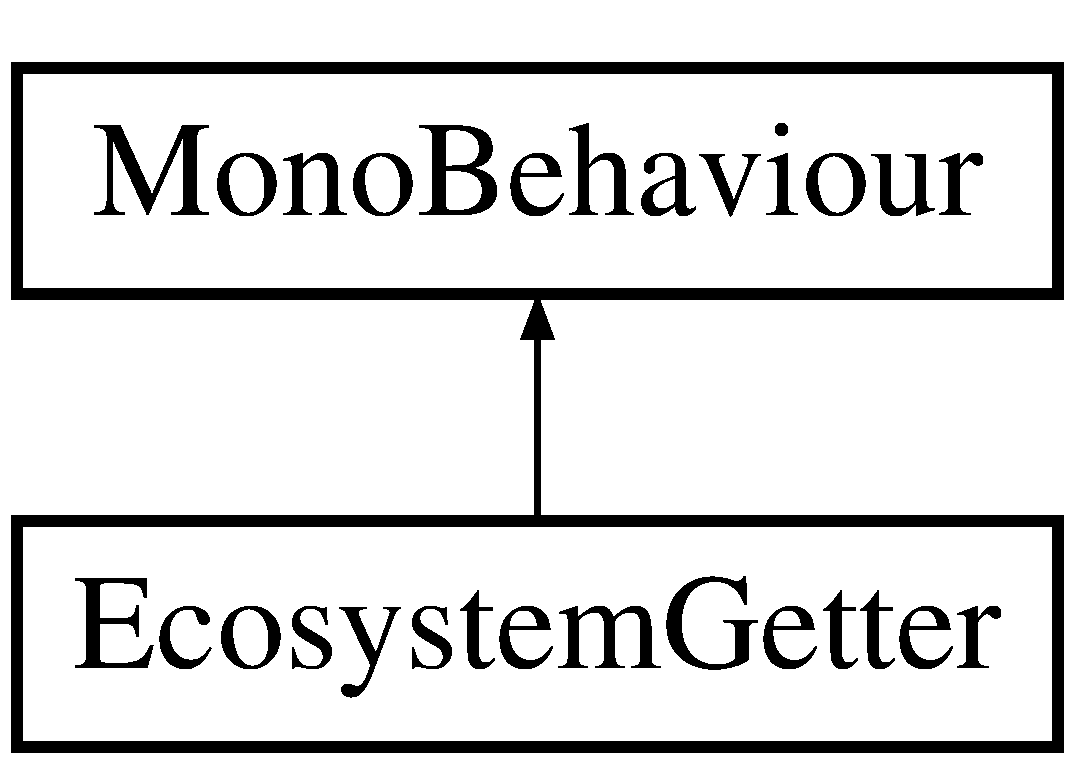
\includegraphics[height=2.000000cm]{class_ecosystem_getter}
\end{center}
\end{figure}
\subsection*{Public Member Functions}
\begin{DoxyCompactItemize}
\item 
int \mbox{\hyperlink{class_ecosystem_getter_a9dab6af6bc871d8e8c6f29bbdcb18483}{get\+Map\+Width}} ()
\item 
int \mbox{\hyperlink{class_ecosystem_getter_abfaba89089f5c6095ca138168a630732}{get\+Map\+Height}} ()
\end{DoxyCompactItemize}
\subsection*{Public Attributes}
\begin{DoxyCompactItemize}
\item 
Game\+Object \mbox{\hyperlink{class_ecosystem_getter_a2a8755cd95e4f94ee8924c699e63a2b8}{sim\+Runner\+Obj}}
\end{DoxyCompactItemize}


\subsection{Member Function Documentation}
\mbox{\Hypertarget{class_ecosystem_getter_abfaba89089f5c6095ca138168a630732}\label{class_ecosystem_getter_abfaba89089f5c6095ca138168a630732}} 
\index{Ecosystem\+Getter@{Ecosystem\+Getter}!get\+Map\+Height@{get\+Map\+Height}}
\index{get\+Map\+Height@{get\+Map\+Height}!Ecosystem\+Getter@{Ecosystem\+Getter}}
\subsubsection{\texorpdfstring{get\+Map\+Height()}{getMapHeight()}}
{\footnotesize\ttfamily int Ecosystem\+Getter.\+get\+Map\+Height (\begin{DoxyParamCaption}{ }\end{DoxyParamCaption})}

\mbox{\Hypertarget{class_ecosystem_getter_a9dab6af6bc871d8e8c6f29bbdcb18483}\label{class_ecosystem_getter_a9dab6af6bc871d8e8c6f29bbdcb18483}} 
\index{Ecosystem\+Getter@{Ecosystem\+Getter}!get\+Map\+Width@{get\+Map\+Width}}
\index{get\+Map\+Width@{get\+Map\+Width}!Ecosystem\+Getter@{Ecosystem\+Getter}}
\subsubsection{\texorpdfstring{get\+Map\+Width()}{getMapWidth()}}
{\footnotesize\ttfamily int Ecosystem\+Getter.\+get\+Map\+Width (\begin{DoxyParamCaption}{ }\end{DoxyParamCaption})}



\subsection{Member Data Documentation}
\mbox{\Hypertarget{class_ecosystem_getter_a2a8755cd95e4f94ee8924c699e63a2b8}\label{class_ecosystem_getter_a2a8755cd95e4f94ee8924c699e63a2b8}} 
\index{Ecosystem\+Getter@{Ecosystem\+Getter}!sim\+Runner\+Obj@{sim\+Runner\+Obj}}
\index{sim\+Runner\+Obj@{sim\+Runner\+Obj}!Ecosystem\+Getter@{Ecosystem\+Getter}}
\subsubsection{\texorpdfstring{sim\+Runner\+Obj}{simRunnerObj}}
{\footnotesize\ttfamily Game\+Object Ecosystem\+Getter.\+sim\+Runner\+Obj}



The documentation for this class was generated from the following file\+:\begin{DoxyCompactItemize}
\item 
\mbox{\hyperlink{_ecosystem_getter_8cs}{Ecosystem\+Getter.\+cs}}\end{DoxyCompactItemize}

\hypertarget{class_empty_activ_behavior}{}\section{Empty\+Activ\+Behavior Class Reference}
\label{class_empty_activ_behavior}\index{Empty\+Activ\+Behavior@{Empty\+Activ\+Behavior}}


No activation function (node simply uses linear combination).  


Inheritance diagram for Empty\+Activ\+Behavior\+:\begin{figure}[H]
\begin{center}
\leavevmode
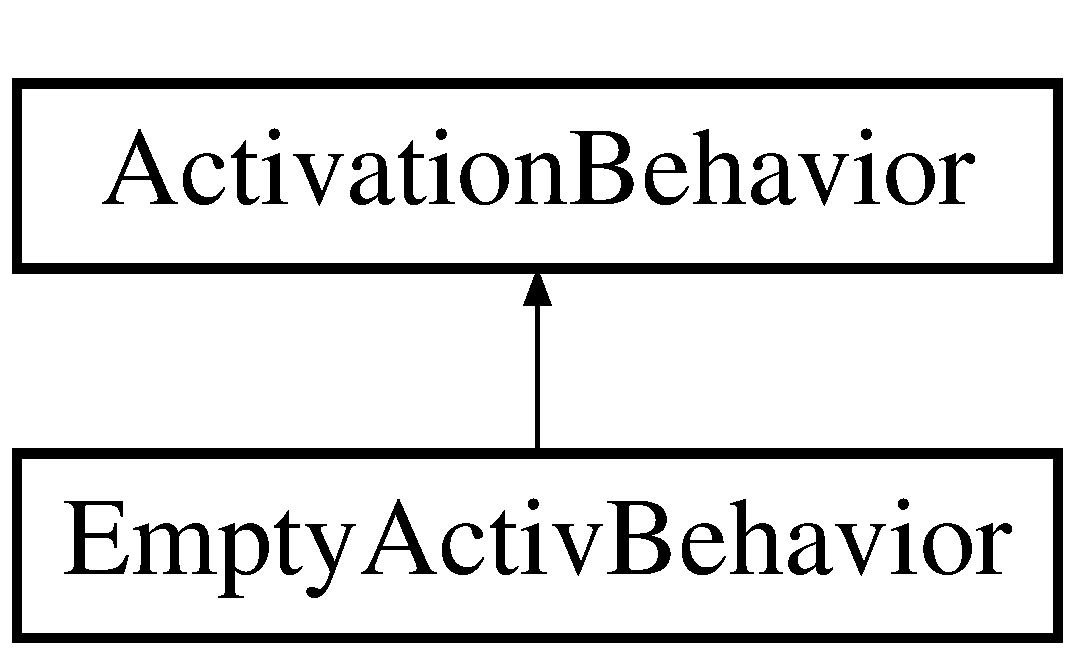
\includegraphics[height=2.000000cm]{class_empty_activ_behavior}
\end{center}
\end{figure}
\subsection*{Public Member Functions}
\begin{DoxyCompactItemize}
\item 
float \mbox{\hyperlink{class_empty_activ_behavior_acc640ba59f2c258030501f8ec9c537d8}{activ\+Funct}} (float input)
\end{DoxyCompactItemize}


\subsection{Detailed Description}
No activation function (node simply uses linear combination). 



\subsection{Member Function Documentation}
\mbox{\Hypertarget{class_empty_activ_behavior_acc640ba59f2c258030501f8ec9c537d8}\label{class_empty_activ_behavior_acc640ba59f2c258030501f8ec9c537d8}} 
\index{Empty\+Activ\+Behavior@{Empty\+Activ\+Behavior}!activ\+Funct@{activ\+Funct}}
\index{activ\+Funct@{activ\+Funct}!Empty\+Activ\+Behavior@{Empty\+Activ\+Behavior}}
\subsubsection{\texorpdfstring{activ\+Funct()}{activFunct()}}
{\footnotesize\ttfamily float Empty\+Activ\+Behavior.\+activ\+Funct (\begin{DoxyParamCaption}\item[{float}]{input }\end{DoxyParamCaption})}



Implements \mbox{\hyperlink{interface_activation_behavior_a6c7af51cf1b10eaadcbf086231e5539b}{Activation\+Behavior}}.



The documentation for this class was generated from the following file\+:\begin{DoxyCompactItemize}
\item 
\mbox{\hyperlink{_empty_activ_behavior_8cs}{Empty\+Activ\+Behavior.\+cs}}\end{DoxyCompactItemize}

\hypertarget{class_error_manager}{}\section{Error\+Manager Class Reference}
\label{class_error_manager}\index{Error\+Manager@{Error\+Manager}}
Inheritance diagram for Error\+Manager\+:\begin{figure}[H]
\begin{center}
\leavevmode
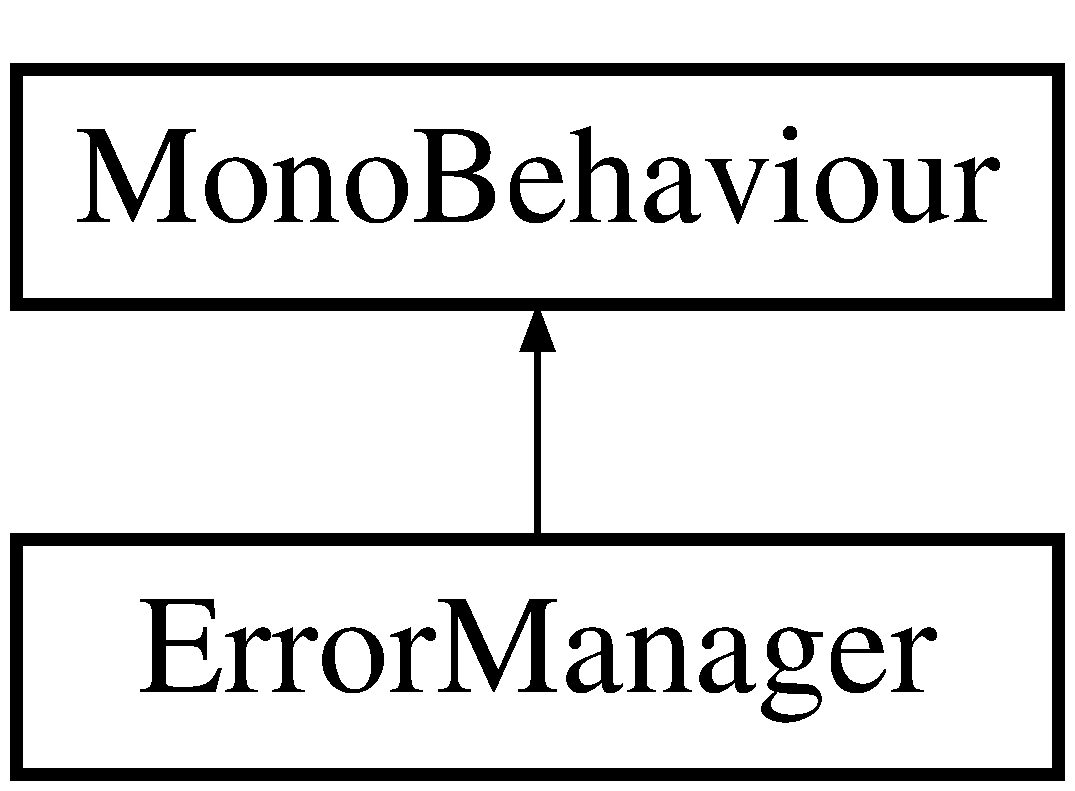
\includegraphics[height=2.000000cm]{class_error_manager}
\end{center}
\end{figure}
\subsection*{Public Attributes}
\begin{DoxyCompactItemize}
\item 
Game\+Object \mbox{\hyperlink{class_error_manager_af503072edfca5b93a809467d35e37677}{error\+Obj}}
\end{DoxyCompactItemize}


\subsection{Member Data Documentation}
\mbox{\Hypertarget{class_error_manager_af503072edfca5b93a809467d35e37677}\label{class_error_manager_af503072edfca5b93a809467d35e37677}} 
\index{Error\+Manager@{Error\+Manager}!error\+Obj@{error\+Obj}}
\index{error\+Obj@{error\+Obj}!Error\+Manager@{Error\+Manager}}
\subsubsection{\texorpdfstring{error\+Obj}{errorObj}}
{\footnotesize\ttfamily Game\+Object Error\+Manager.\+error\+Obj}



The documentation for this class was generated from the following file\+:\begin{DoxyCompactItemize}
\item 
\mbox{\hyperlink{_error_manager_8cs}{Error\+Manager.\+cs}}\end{DoxyCompactItemize}

\hypertarget{class_game_manager}{}\section{Game\+Manager Class Reference}
\label{class_game_manager}\index{Game\+Manager@{Game\+Manager}}
Inheritance diagram for Game\+Manager\+:\begin{figure}[H]
\begin{center}
\leavevmode
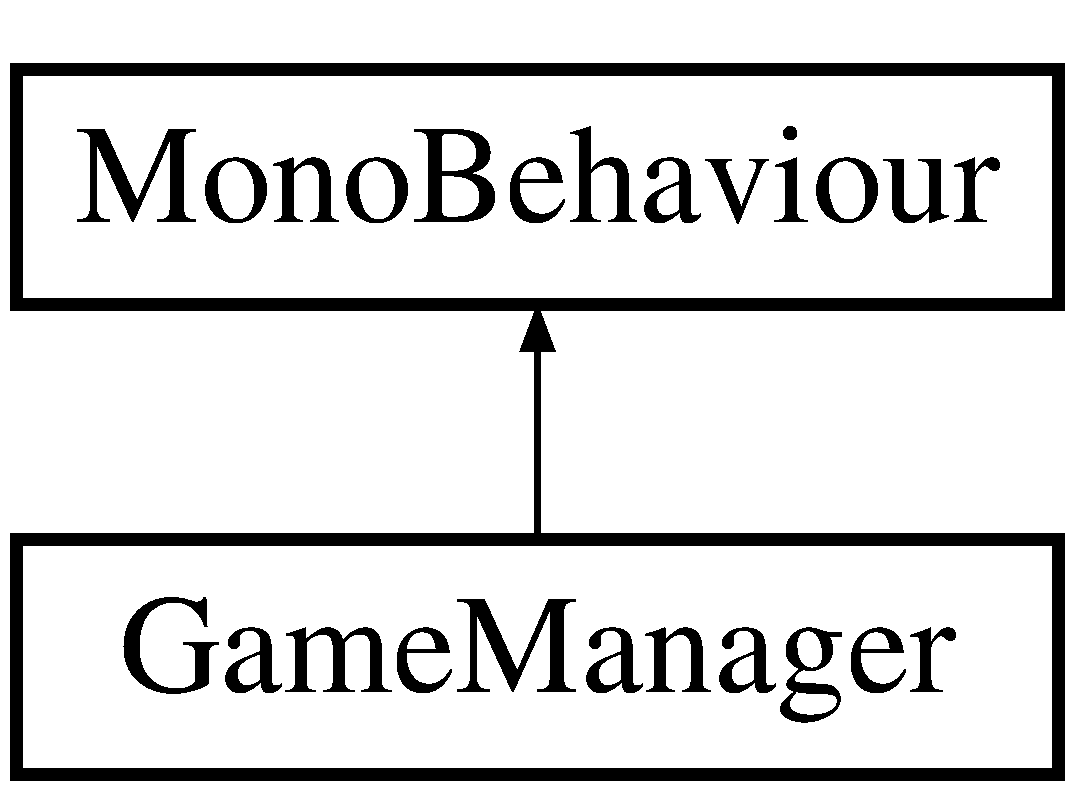
\includegraphics[height=2.000000cm]{class_game_manager}
\end{center}
\end{figure}
\subsection*{Public Member Functions}
\begin{DoxyCompactItemize}
\item 
void \mbox{\hyperlink{class_game_manager_a5ccfacd027ad08eeb4ff1f25a7f59c98}{Start}} ()
\item 
void \mbox{\hyperlink{class_game_manager_a5ef457428a5dca16616bd717a7e5aec9}{add\+Ecosystem}} (\mbox{\hyperlink{class_ecosystem}{Ecosystem}} eco)
\item 
void \mbox{\hyperlink{class_game_manager_ae6f288a4230d1cf2e5ed42614fcfc12a}{start\+User\+Simulation}} (int sim\+Steps)
\end{DoxyCompactItemize}


\subsection{Member Function Documentation}
\mbox{\Hypertarget{class_game_manager_a5ef457428a5dca16616bd717a7e5aec9}\label{class_game_manager_a5ef457428a5dca16616bd717a7e5aec9}} 
\index{Game\+Manager@{Game\+Manager}!add\+Ecosystem@{add\+Ecosystem}}
\index{add\+Ecosystem@{add\+Ecosystem}!Game\+Manager@{Game\+Manager}}
\subsubsection{\texorpdfstring{add\+Ecosystem()}{addEcosystem()}}
{\footnotesize\ttfamily void Game\+Manager.\+add\+Ecosystem (\begin{DoxyParamCaption}\item[{\mbox{\hyperlink{class_ecosystem}{Ecosystem}}}]{eco }\end{DoxyParamCaption})}

\mbox{\Hypertarget{class_game_manager_a5ccfacd027ad08eeb4ff1f25a7f59c98}\label{class_game_manager_a5ccfacd027ad08eeb4ff1f25a7f59c98}} 
\index{Game\+Manager@{Game\+Manager}!Start@{Start}}
\index{Start@{Start}!Game\+Manager@{Game\+Manager}}
\subsubsection{\texorpdfstring{Start()}{Start()}}
{\footnotesize\ttfamily void Game\+Manager.\+Start (\begin{DoxyParamCaption}{ }\end{DoxyParamCaption})}

\mbox{\Hypertarget{class_game_manager_ae6f288a4230d1cf2e5ed42614fcfc12a}\label{class_game_manager_ae6f288a4230d1cf2e5ed42614fcfc12a}} 
\index{Game\+Manager@{Game\+Manager}!start\+User\+Simulation@{start\+User\+Simulation}}
\index{start\+User\+Simulation@{start\+User\+Simulation}!Game\+Manager@{Game\+Manager}}
\subsubsection{\texorpdfstring{start\+User\+Simulation()}{startUserSimulation()}}
{\footnotesize\ttfamily void Game\+Manager.\+start\+User\+Simulation (\begin{DoxyParamCaption}\item[{int}]{sim\+Steps }\end{DoxyParamCaption})}



The documentation for this class was generated from the following file\+:\begin{DoxyCompactItemize}
\item 
\mbox{\hyperlink{_game_manager_8cs}{Game\+Manager.\+cs}}\end{DoxyCompactItemize}

\hypertarget{class_helper_validator}{}\section{Helper\+Validator Class Reference}
\label{class_helper_validator}\index{Helper\+Validator@{Helper\+Validator}}
\subsection*{Static Public Member Functions}
\begin{DoxyCompactItemize}
\item 
static bool \mbox{\hyperlink{class_helper_validator_ae2a4197b74ecf12c37770790da74149f}{validate\+Integer\+String}} (string text)
\item 
static bool \mbox{\hyperlink{class_helper_validator_a655881eabb458927f86ff12201f68ba1}{validate\+Float\+String}} (string text)
\item 
static bool \mbox{\hyperlink{class_helper_validator_adabea3639000268b6d2a12a2b9c17eaf}{set\+Integer\+Funct}} (Game\+Object go, \mbox{\hyperlink{_helper_validator_8cs_a39d82d930145ffb7e5326699e0ef7f27}{Int\+Funct}} set\+Int, Game\+Object \mbox{\hyperlink{class_helper_validator_aa83d9143271cabe1e41f61d94304c960}{error\+Obj}})
\item 
static bool \mbox{\hyperlink{class_helper_validator_ac0d529df7419bf6aec6754c43565d4cc}{set\+Name}} (Game\+Object text\+Box, Game\+Object \mbox{\hyperlink{class_helper_validator_aa83d9143271cabe1e41f61d94304c960}{error\+Obj}}, \mbox{\hyperlink{_helper_validator_8cs_a960dfdb4c2811fe6c539a15632075939}{String\+Funct}} string\+Setter)
\end{DoxyCompactItemize}
\subsection*{Static Public Attributes}
\begin{DoxyCompactItemize}
\item 
static Game\+Object \mbox{\hyperlink{class_helper_validator_aa83d9143271cabe1e41f61d94304c960}{error\+Obj}}
\end{DoxyCompactItemize}


\subsection{Member Function Documentation}
\mbox{\Hypertarget{class_helper_validator_adabea3639000268b6d2a12a2b9c17eaf}\label{class_helper_validator_adabea3639000268b6d2a12a2b9c17eaf}} 
\index{Helper\+Validator@{Helper\+Validator}!set\+Integer\+Funct@{set\+Integer\+Funct}}
\index{set\+Integer\+Funct@{set\+Integer\+Funct}!Helper\+Validator@{Helper\+Validator}}
\subsubsection{\texorpdfstring{set\+Integer\+Funct()}{setIntegerFunct()}}
{\footnotesize\ttfamily static bool Helper\+Validator.\+set\+Integer\+Funct (\begin{DoxyParamCaption}\item[{Game\+Object}]{go,  }\item[{\mbox{\hyperlink{_helper_validator_8cs_a39d82d930145ffb7e5326699e0ef7f27}{Int\+Funct}}}]{set\+Int,  }\item[{Game\+Object}]{error\+Obj }\end{DoxyParamCaption})\hspace{0.3cm}{\ttfamily [static]}}

\mbox{\Hypertarget{class_helper_validator_ac0d529df7419bf6aec6754c43565d4cc}\label{class_helper_validator_ac0d529df7419bf6aec6754c43565d4cc}} 
\index{Helper\+Validator@{Helper\+Validator}!set\+Name@{set\+Name}}
\index{set\+Name@{set\+Name}!Helper\+Validator@{Helper\+Validator}}
\subsubsection{\texorpdfstring{set\+Name()}{setName()}}
{\footnotesize\ttfamily static bool Helper\+Validator.\+set\+Name (\begin{DoxyParamCaption}\item[{Game\+Object}]{text\+Box,  }\item[{Game\+Object}]{error\+Obj,  }\item[{\mbox{\hyperlink{_helper_validator_8cs_a960dfdb4c2811fe6c539a15632075939}{String\+Funct}}}]{string\+Setter }\end{DoxyParamCaption})\hspace{0.3cm}{\ttfamily [static]}}

\mbox{\Hypertarget{class_helper_validator_a655881eabb458927f86ff12201f68ba1}\label{class_helper_validator_a655881eabb458927f86ff12201f68ba1}} 
\index{Helper\+Validator@{Helper\+Validator}!validate\+Float\+String@{validate\+Float\+String}}
\index{validate\+Float\+String@{validate\+Float\+String}!Helper\+Validator@{Helper\+Validator}}
\subsubsection{\texorpdfstring{validate\+Float\+String()}{validateFloatString()}}
{\footnotesize\ttfamily static bool Helper\+Validator.\+validate\+Float\+String (\begin{DoxyParamCaption}\item[{string}]{text }\end{DoxyParamCaption})\hspace{0.3cm}{\ttfamily [static]}}

\mbox{\Hypertarget{class_helper_validator_ae2a4197b74ecf12c37770790da74149f}\label{class_helper_validator_ae2a4197b74ecf12c37770790da74149f}} 
\index{Helper\+Validator@{Helper\+Validator}!validate\+Integer\+String@{validate\+Integer\+String}}
\index{validate\+Integer\+String@{validate\+Integer\+String}!Helper\+Validator@{Helper\+Validator}}
\subsubsection{\texorpdfstring{validate\+Integer\+String()}{validateIntegerString()}}
{\footnotesize\ttfamily static bool Helper\+Validator.\+validate\+Integer\+String (\begin{DoxyParamCaption}\item[{string}]{text }\end{DoxyParamCaption})\hspace{0.3cm}{\ttfamily [static]}}



\subsection{Member Data Documentation}
\mbox{\Hypertarget{class_helper_validator_aa83d9143271cabe1e41f61d94304c960}\label{class_helper_validator_aa83d9143271cabe1e41f61d94304c960}} 
\index{Helper\+Validator@{Helper\+Validator}!error\+Obj@{error\+Obj}}
\index{error\+Obj@{error\+Obj}!Helper\+Validator@{Helper\+Validator}}
\subsubsection{\texorpdfstring{error\+Obj}{errorObj}}
{\footnotesize\ttfamily Game\+Object Helper\+Validator.\+error\+Obj\hspace{0.3cm}{\ttfamily [static]}}



The documentation for this class was generated from the following file\+:\begin{DoxyCompactItemize}
\item 
\mbox{\hyperlink{_helper_validator_8cs}{Helper\+Validator.\+cs}}\end{DoxyCompactItemize}

\hypertarget{interface_i_ecosystem_editor}{}\section{I\+Ecosystem\+Editor Interface Reference}
\label{interface_i_ecosystem_editor}\index{I\+Ecosystem\+Editor@{I\+Ecosystem\+Editor}}
\subsection*{Public Member Functions}
\begin{DoxyCompactItemize}
\item 
\mbox{\hyperlink{class_creature_editor}{Creature\+Editor}} \mbox{\hyperlink{interface_i_ecosystem_editor_aaae20f895373be5be6f31b6f93bbfd0b}{add\+Creature}} ()
\item 
void \mbox{\hyperlink{interface_i_ecosystem_editor_ab6545a2061db61dcb2d2dd05da18957e}{add\+Current\+Population\+To\+Ecosystem}} ()
\item 
void \mbox{\hyperlink{interface_i_ecosystem_editor_ac4a3d0d62cbb3e2c5df3f053b2527f1c}{add\+Current\+Population\+To\+Map}} ()
\item 
void \mbox{\hyperlink{interface_i_ecosystem_editor_a41508804136106839c9715c7c26ae1b0}{add\+Resource}} (string resource\+Name)
\item 
void \mbox{\hyperlink{interface_i_ecosystem_editor_a63ed483beb9eaee554e2cdc4355d120a}{add\+To\+Founders}} ()
\item 
\mbox{\hyperlink{class_species_populator}{Species\+Populator}} \mbox{\hyperlink{interface_i_ecosystem_editor_ac69c303518bbb0f6990fb6927d6ae1fb}{populate\+Species}} (string founder\+Species)
\item 
void \mbox{\hyperlink{interface_i_ecosystem_editor_a5f37487f43114680ba0b0673662a6110}{save\+Current\+Population}} ()
\item 
void \mbox{\hyperlink{interface_i_ecosystem_editor_a2837b080f668269248f47a11e14425ea}{save\+Edited\+Map}} ()
\item 
void \mbox{\hyperlink{interface_i_ecosystem_editor_a1030121515b424e576fe33d8a3590fd7}{save\+Founders\+To\+Species}} ()
\item 
void \mbox{\hyperlink{interface_i_ecosystem_editor_a293320f7cb1ea2b228339f6a44e8fe8b}{save\+Map}} ()
\item 
void \mbox{\hyperlink{interface_i_ecosystem_editor_a04d432f43910eb38f45f68ff3a6a52a0}{save\+Resource}} ()
\item 
void \mbox{\hyperlink{interface_i_ecosystem_editor_a673154ec9f666f6bf5b25c5767d5de46}{save\+Resource\+Options}} ()
\item 
void \mbox{\hyperlink{interface_i_ecosystem_editor_ae4e824dc976d499010849d8d7d9fb730}{set\+Ability\+Points\+Per\+Creature}} (int ability\+Points)
\item 
void \mbox{\hyperlink{interface_i_ecosystem_editor_a61e02c9c45d6cff7f8d2b2760eeba1dc}{set\+Comm\+Bits}} (int num\+Bits)
\item 
void \mbox{\hyperlink{interface_i_ecosystem_editor_af81453db6f44e7276ba5467c5b582527}{set\+Distinct\+Phenotype\+Num}} (int num\+Phenotypes)
\item 
void \mbox{\hyperlink{interface_i_ecosystem_editor_a4dabd8d8fcf4acab6e2345675a33724a}{set\+Name}} (string name)
\item 
void \mbox{\hyperlink{interface_i_ecosystem_editor_ae05ed2195503dc3ee2aee5ef61116039}{set\+Time\+Units\+Per\+Turn}} (int time\+Units)
\end{DoxyCompactItemize}


\subsection{Member Function Documentation}
\mbox{\Hypertarget{interface_i_ecosystem_editor_aaae20f895373be5be6f31b6f93bbfd0b}\label{interface_i_ecosystem_editor_aaae20f895373be5be6f31b6f93bbfd0b}} 
\index{I\+Ecosystem\+Editor@{I\+Ecosystem\+Editor}!add\+Creature@{add\+Creature}}
\index{add\+Creature@{add\+Creature}!I\+Ecosystem\+Editor@{I\+Ecosystem\+Editor}}
\subsubsection{\texorpdfstring{add\+Creature()}{addCreature()}}
{\footnotesize\ttfamily \mbox{\hyperlink{class_creature_editor}{Creature\+Editor}} I\+Ecosystem\+Editor.\+add\+Creature (\begin{DoxyParamCaption}{ }\end{DoxyParamCaption})}

\mbox{\Hypertarget{interface_i_ecosystem_editor_ab6545a2061db61dcb2d2dd05da18957e}\label{interface_i_ecosystem_editor_ab6545a2061db61dcb2d2dd05da18957e}} 
\index{I\+Ecosystem\+Editor@{I\+Ecosystem\+Editor}!add\+Current\+Population\+To\+Ecosystem@{add\+Current\+Population\+To\+Ecosystem}}
\index{add\+Current\+Population\+To\+Ecosystem@{add\+Current\+Population\+To\+Ecosystem}!I\+Ecosystem\+Editor@{I\+Ecosystem\+Editor}}
\subsubsection{\texorpdfstring{add\+Current\+Population\+To\+Ecosystem()}{addCurrentPopulationToEcosystem()}}
{\footnotesize\ttfamily void I\+Ecosystem\+Editor.\+add\+Current\+Population\+To\+Ecosystem (\begin{DoxyParamCaption}{ }\end{DoxyParamCaption})}

\mbox{\Hypertarget{interface_i_ecosystem_editor_ac4a3d0d62cbb3e2c5df3f053b2527f1c}\label{interface_i_ecosystem_editor_ac4a3d0d62cbb3e2c5df3f053b2527f1c}} 
\index{I\+Ecosystem\+Editor@{I\+Ecosystem\+Editor}!add\+Current\+Population\+To\+Map@{add\+Current\+Population\+To\+Map}}
\index{add\+Current\+Population\+To\+Map@{add\+Current\+Population\+To\+Map}!I\+Ecosystem\+Editor@{I\+Ecosystem\+Editor}}
\subsubsection{\texorpdfstring{add\+Current\+Population\+To\+Map()}{addCurrentPopulationToMap()}}
{\footnotesize\ttfamily void I\+Ecosystem\+Editor.\+add\+Current\+Population\+To\+Map (\begin{DoxyParamCaption}{ }\end{DoxyParamCaption})}

\mbox{\Hypertarget{interface_i_ecosystem_editor_a41508804136106839c9715c7c26ae1b0}\label{interface_i_ecosystem_editor_a41508804136106839c9715c7c26ae1b0}} 
\index{I\+Ecosystem\+Editor@{I\+Ecosystem\+Editor}!add\+Resource@{add\+Resource}}
\index{add\+Resource@{add\+Resource}!I\+Ecosystem\+Editor@{I\+Ecosystem\+Editor}}
\subsubsection{\texorpdfstring{add\+Resource()}{addResource()}}
{\footnotesize\ttfamily void I\+Ecosystem\+Editor.\+add\+Resource (\begin{DoxyParamCaption}\item[{string}]{resource\+Name }\end{DoxyParamCaption})}

\mbox{\Hypertarget{interface_i_ecosystem_editor_a63ed483beb9eaee554e2cdc4355d120a}\label{interface_i_ecosystem_editor_a63ed483beb9eaee554e2cdc4355d120a}} 
\index{I\+Ecosystem\+Editor@{I\+Ecosystem\+Editor}!add\+To\+Founders@{add\+To\+Founders}}
\index{add\+To\+Founders@{add\+To\+Founders}!I\+Ecosystem\+Editor@{I\+Ecosystem\+Editor}}
\subsubsection{\texorpdfstring{add\+To\+Founders()}{addToFounders()}}
{\footnotesize\ttfamily void I\+Ecosystem\+Editor.\+add\+To\+Founders (\begin{DoxyParamCaption}{ }\end{DoxyParamCaption})}

\mbox{\Hypertarget{interface_i_ecosystem_editor_ac69c303518bbb0f6990fb6927d6ae1fb}\label{interface_i_ecosystem_editor_ac69c303518bbb0f6990fb6927d6ae1fb}} 
\index{I\+Ecosystem\+Editor@{I\+Ecosystem\+Editor}!populate\+Species@{populate\+Species}}
\index{populate\+Species@{populate\+Species}!I\+Ecosystem\+Editor@{I\+Ecosystem\+Editor}}
\subsubsection{\texorpdfstring{populate\+Species()}{populateSpecies()}}
{\footnotesize\ttfamily \mbox{\hyperlink{class_species_populator}{Species\+Populator}} I\+Ecosystem\+Editor.\+populate\+Species (\begin{DoxyParamCaption}\item[{string}]{founder\+Species }\end{DoxyParamCaption})}

\mbox{\Hypertarget{interface_i_ecosystem_editor_a5f37487f43114680ba0b0673662a6110}\label{interface_i_ecosystem_editor_a5f37487f43114680ba0b0673662a6110}} 
\index{I\+Ecosystem\+Editor@{I\+Ecosystem\+Editor}!save\+Current\+Population@{save\+Current\+Population}}
\index{save\+Current\+Population@{save\+Current\+Population}!I\+Ecosystem\+Editor@{I\+Ecosystem\+Editor}}
\subsubsection{\texorpdfstring{save\+Current\+Population()}{saveCurrentPopulation()}}
{\footnotesize\ttfamily void I\+Ecosystem\+Editor.\+save\+Current\+Population (\begin{DoxyParamCaption}{ }\end{DoxyParamCaption})}

\mbox{\Hypertarget{interface_i_ecosystem_editor_a2837b080f668269248f47a11e14425ea}\label{interface_i_ecosystem_editor_a2837b080f668269248f47a11e14425ea}} 
\index{I\+Ecosystem\+Editor@{I\+Ecosystem\+Editor}!save\+Edited\+Map@{save\+Edited\+Map}}
\index{save\+Edited\+Map@{save\+Edited\+Map}!I\+Ecosystem\+Editor@{I\+Ecosystem\+Editor}}
\subsubsection{\texorpdfstring{save\+Edited\+Map()}{saveEditedMap()}}
{\footnotesize\ttfamily void I\+Ecosystem\+Editor.\+save\+Edited\+Map (\begin{DoxyParamCaption}{ }\end{DoxyParamCaption})}

\mbox{\Hypertarget{interface_i_ecosystem_editor_a1030121515b424e576fe33d8a3590fd7}\label{interface_i_ecosystem_editor_a1030121515b424e576fe33d8a3590fd7}} 
\index{I\+Ecosystem\+Editor@{I\+Ecosystem\+Editor}!save\+Founders\+To\+Species@{save\+Founders\+To\+Species}}
\index{save\+Founders\+To\+Species@{save\+Founders\+To\+Species}!I\+Ecosystem\+Editor@{I\+Ecosystem\+Editor}}
\subsubsection{\texorpdfstring{save\+Founders\+To\+Species()}{saveFoundersToSpecies()}}
{\footnotesize\ttfamily void I\+Ecosystem\+Editor.\+save\+Founders\+To\+Species (\begin{DoxyParamCaption}{ }\end{DoxyParamCaption})}

\mbox{\Hypertarget{interface_i_ecosystem_editor_a293320f7cb1ea2b228339f6a44e8fe8b}\label{interface_i_ecosystem_editor_a293320f7cb1ea2b228339f6a44e8fe8b}} 
\index{I\+Ecosystem\+Editor@{I\+Ecosystem\+Editor}!save\+Map@{save\+Map}}
\index{save\+Map@{save\+Map}!I\+Ecosystem\+Editor@{I\+Ecosystem\+Editor}}
\subsubsection{\texorpdfstring{save\+Map()}{saveMap()}}
{\footnotesize\ttfamily void I\+Ecosystem\+Editor.\+save\+Map (\begin{DoxyParamCaption}{ }\end{DoxyParamCaption})}

\mbox{\Hypertarget{interface_i_ecosystem_editor_a04d432f43910eb38f45f68ff3a6a52a0}\label{interface_i_ecosystem_editor_a04d432f43910eb38f45f68ff3a6a52a0}} 
\index{I\+Ecosystem\+Editor@{I\+Ecosystem\+Editor}!save\+Resource@{save\+Resource}}
\index{save\+Resource@{save\+Resource}!I\+Ecosystem\+Editor@{I\+Ecosystem\+Editor}}
\subsubsection{\texorpdfstring{save\+Resource()}{saveResource()}}
{\footnotesize\ttfamily void I\+Ecosystem\+Editor.\+save\+Resource (\begin{DoxyParamCaption}{ }\end{DoxyParamCaption})}

\mbox{\Hypertarget{interface_i_ecosystem_editor_a673154ec9f666f6bf5b25c5767d5de46}\label{interface_i_ecosystem_editor_a673154ec9f666f6bf5b25c5767d5de46}} 
\index{I\+Ecosystem\+Editor@{I\+Ecosystem\+Editor}!save\+Resource\+Options@{save\+Resource\+Options}}
\index{save\+Resource\+Options@{save\+Resource\+Options}!I\+Ecosystem\+Editor@{I\+Ecosystem\+Editor}}
\subsubsection{\texorpdfstring{save\+Resource\+Options()}{saveResourceOptions()}}
{\footnotesize\ttfamily void I\+Ecosystem\+Editor.\+save\+Resource\+Options (\begin{DoxyParamCaption}{ }\end{DoxyParamCaption})}

\mbox{\Hypertarget{interface_i_ecosystem_editor_ae4e824dc976d499010849d8d7d9fb730}\label{interface_i_ecosystem_editor_ae4e824dc976d499010849d8d7d9fb730}} 
\index{I\+Ecosystem\+Editor@{I\+Ecosystem\+Editor}!set\+Ability\+Points\+Per\+Creature@{set\+Ability\+Points\+Per\+Creature}}
\index{set\+Ability\+Points\+Per\+Creature@{set\+Ability\+Points\+Per\+Creature}!I\+Ecosystem\+Editor@{I\+Ecosystem\+Editor}}
\subsubsection{\texorpdfstring{set\+Ability\+Points\+Per\+Creature()}{setAbilityPointsPerCreature()}}
{\footnotesize\ttfamily void I\+Ecosystem\+Editor.\+set\+Ability\+Points\+Per\+Creature (\begin{DoxyParamCaption}\item[{int}]{ability\+Points }\end{DoxyParamCaption})}

\mbox{\Hypertarget{interface_i_ecosystem_editor_a61e02c9c45d6cff7f8d2b2760eeba1dc}\label{interface_i_ecosystem_editor_a61e02c9c45d6cff7f8d2b2760eeba1dc}} 
\index{I\+Ecosystem\+Editor@{I\+Ecosystem\+Editor}!set\+Comm\+Bits@{set\+Comm\+Bits}}
\index{set\+Comm\+Bits@{set\+Comm\+Bits}!I\+Ecosystem\+Editor@{I\+Ecosystem\+Editor}}
\subsubsection{\texorpdfstring{set\+Comm\+Bits()}{setCommBits()}}
{\footnotesize\ttfamily void I\+Ecosystem\+Editor.\+set\+Comm\+Bits (\begin{DoxyParamCaption}\item[{int}]{num\+Bits }\end{DoxyParamCaption})}

\mbox{\Hypertarget{interface_i_ecosystem_editor_af81453db6f44e7276ba5467c5b582527}\label{interface_i_ecosystem_editor_af81453db6f44e7276ba5467c5b582527}} 
\index{I\+Ecosystem\+Editor@{I\+Ecosystem\+Editor}!set\+Distinct\+Phenotype\+Num@{set\+Distinct\+Phenotype\+Num}}
\index{set\+Distinct\+Phenotype\+Num@{set\+Distinct\+Phenotype\+Num}!I\+Ecosystem\+Editor@{I\+Ecosystem\+Editor}}
\subsubsection{\texorpdfstring{set\+Distinct\+Phenotype\+Num()}{setDistinctPhenotypeNum()}}
{\footnotesize\ttfamily void I\+Ecosystem\+Editor.\+set\+Distinct\+Phenotype\+Num (\begin{DoxyParamCaption}\item[{int}]{num\+Phenotypes }\end{DoxyParamCaption})}

\mbox{\Hypertarget{interface_i_ecosystem_editor_a4dabd8d8fcf4acab6e2345675a33724a}\label{interface_i_ecosystem_editor_a4dabd8d8fcf4acab6e2345675a33724a}} 
\index{I\+Ecosystem\+Editor@{I\+Ecosystem\+Editor}!set\+Name@{set\+Name}}
\index{set\+Name@{set\+Name}!I\+Ecosystem\+Editor@{I\+Ecosystem\+Editor}}
\subsubsection{\texorpdfstring{set\+Name()}{setName()}}
{\footnotesize\ttfamily void I\+Ecosystem\+Editor.\+set\+Name (\begin{DoxyParamCaption}\item[{string}]{name }\end{DoxyParamCaption})}

\mbox{\Hypertarget{interface_i_ecosystem_editor_ae05ed2195503dc3ee2aee5ef61116039}\label{interface_i_ecosystem_editor_ae05ed2195503dc3ee2aee5ef61116039}} 
\index{I\+Ecosystem\+Editor@{I\+Ecosystem\+Editor}!set\+Time\+Units\+Per\+Turn@{set\+Time\+Units\+Per\+Turn}}
\index{set\+Time\+Units\+Per\+Turn@{set\+Time\+Units\+Per\+Turn}!I\+Ecosystem\+Editor@{I\+Ecosystem\+Editor}}
\subsubsection{\texorpdfstring{set\+Time\+Units\+Per\+Turn()}{setTimeUnitsPerTurn()}}
{\footnotesize\ttfamily void I\+Ecosystem\+Editor.\+set\+Time\+Units\+Per\+Turn (\begin{DoxyParamCaption}\item[{int}]{time\+Units }\end{DoxyParamCaption})}



The documentation for this interface was generated from the following file\+:\begin{DoxyCompactItemize}
\item 
\mbox{\hyperlink{_i_ecosystem_editor_8cs}{I\+Ecosystem\+Editor.\+cs}}\end{DoxyCompactItemize}

\hypertarget{class_inner_input_node}{}\section{Inner\+Input\+Node Class Reference}
\label{class_inner_input_node}\index{Inner\+Input\+Node@{Inner\+Input\+Node}}
Inheritance diagram for Inner\+Input\+Node\+:\begin{figure}[H]
\begin{center}
\leavevmode
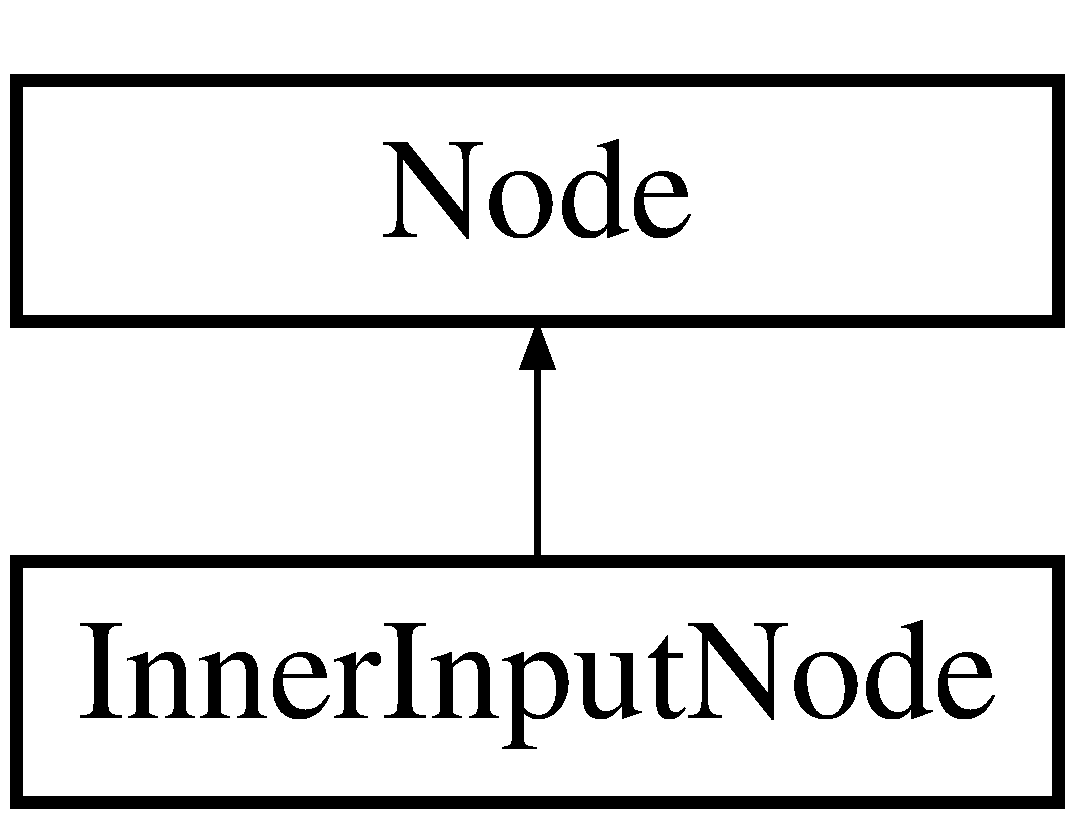
\includegraphics[height=2.000000cm]{class_inner_input_node}
\end{center}
\end{figure}
\subsection*{Public Member Functions}
\begin{DoxyCompactItemize}
\item 
override void \mbox{\hyperlink{class_inner_input_node_ac67f9a1dcd0ae72d2d7fe4cfa7f91152}{update\+Value}} ()
\begin{DoxyCompactList}\small\item\em This method simply gets the value from in\+Node. \end{DoxyCompactList}\item 
\mbox{\hyperlink{class_inner_input_node}{Inner\+Input\+Node}} \mbox{\hyperlink{class_inner_input_node_ae5611efed948ab50400a6204319490a5}{clone}} ()
\end{DoxyCompactItemize}
\subsection*{Public Attributes}
\begin{DoxyCompactItemize}
\item 
\mbox{\hyperlink{class_node}{Node}} \mbox{\hyperlink{class_inner_input_node_a56ef3e3b3b66cac2a74094373a154fc6}{linked\+Node}}
\item 
string \mbox{\hyperlink{class_inner_input_node_a59c3f5f1aacedbf2bebab494d9e75f91}{linked\+Net\+Name}}
\item 
\mbox{\hyperlink{class_creature}{Creature}} \mbox{\hyperlink{class_inner_input_node_adfb709c73b39672d7bcecc0bed14ad5f}{parent\+Creature}}
\item 
int \mbox{\hyperlink{class_inner_input_node_a110568103ae4dc406276330d83be7fad}{linked\+Node\+Index}}
\item 
int \mbox{\hyperlink{class_inner_input_node_a839da78d668a0a301d7bb640ac431082}{linked\+Node\+Network\+Layer}}
\end{DoxyCompactItemize}


\subsection{Member Function Documentation}
\mbox{\Hypertarget{class_inner_input_node_ae5611efed948ab50400a6204319490a5}\label{class_inner_input_node_ae5611efed948ab50400a6204319490a5}} 
\index{Inner\+Input\+Node@{Inner\+Input\+Node}!clone@{clone}}
\index{clone@{clone}!Inner\+Input\+Node@{Inner\+Input\+Node}}
\subsubsection{\texorpdfstring{clone()}{clone()}}
{\footnotesize\ttfamily \mbox{\hyperlink{class_inner_input_node}{Inner\+Input\+Node}} Inner\+Input\+Node.\+clone (\begin{DoxyParamCaption}{ }\end{DoxyParamCaption})}

\mbox{\Hypertarget{class_inner_input_node_ac67f9a1dcd0ae72d2d7fe4cfa7f91152}\label{class_inner_input_node_ac67f9a1dcd0ae72d2d7fe4cfa7f91152}} 
\index{Inner\+Input\+Node@{Inner\+Input\+Node}!update\+Value@{update\+Value}}
\index{update\+Value@{update\+Value}!Inner\+Input\+Node@{Inner\+Input\+Node}}
\subsubsection{\texorpdfstring{update\+Value()}{updateValue()}}
{\footnotesize\ttfamily override void Inner\+Input\+Node.\+update\+Value (\begin{DoxyParamCaption}{ }\end{DoxyParamCaption})\hspace{0.3cm}{\ttfamily [virtual]}}



This method simply gets the value from in\+Node. 



Implements \mbox{\hyperlink{class_node_a85ebd0e36c25430570b94f923afd2a62}{Node}}.



\subsection{Member Data Documentation}
\mbox{\Hypertarget{class_inner_input_node_a59c3f5f1aacedbf2bebab494d9e75f91}\label{class_inner_input_node_a59c3f5f1aacedbf2bebab494d9e75f91}} 
\index{Inner\+Input\+Node@{Inner\+Input\+Node}!linked\+Net\+Name@{linked\+Net\+Name}}
\index{linked\+Net\+Name@{linked\+Net\+Name}!Inner\+Input\+Node@{Inner\+Input\+Node}}
\subsubsection{\texorpdfstring{linked\+Net\+Name}{linkedNetName}}
{\footnotesize\ttfamily string Inner\+Input\+Node.\+linked\+Net\+Name}

\mbox{\Hypertarget{class_inner_input_node_a56ef3e3b3b66cac2a74094373a154fc6}\label{class_inner_input_node_a56ef3e3b3b66cac2a74094373a154fc6}} 
\index{Inner\+Input\+Node@{Inner\+Input\+Node}!linked\+Node@{linked\+Node}}
\index{linked\+Node@{linked\+Node}!Inner\+Input\+Node@{Inner\+Input\+Node}}
\subsubsection{\texorpdfstring{linked\+Node}{linkedNode}}
{\footnotesize\ttfamily \mbox{\hyperlink{class_node}{Node}} Inner\+Input\+Node.\+linked\+Node}

\mbox{\Hypertarget{class_inner_input_node_a110568103ae4dc406276330d83be7fad}\label{class_inner_input_node_a110568103ae4dc406276330d83be7fad}} 
\index{Inner\+Input\+Node@{Inner\+Input\+Node}!linked\+Node\+Index@{linked\+Node\+Index}}
\index{linked\+Node\+Index@{linked\+Node\+Index}!Inner\+Input\+Node@{Inner\+Input\+Node}}
\subsubsection{\texorpdfstring{linked\+Node\+Index}{linkedNodeIndex}}
{\footnotesize\ttfamily int Inner\+Input\+Node.\+linked\+Node\+Index}

\mbox{\Hypertarget{class_inner_input_node_a839da78d668a0a301d7bb640ac431082}\label{class_inner_input_node_a839da78d668a0a301d7bb640ac431082}} 
\index{Inner\+Input\+Node@{Inner\+Input\+Node}!linked\+Node\+Network\+Layer@{linked\+Node\+Network\+Layer}}
\index{linked\+Node\+Network\+Layer@{linked\+Node\+Network\+Layer}!Inner\+Input\+Node@{Inner\+Input\+Node}}
\subsubsection{\texorpdfstring{linked\+Node\+Network\+Layer}{linkedNodeNetworkLayer}}
{\footnotesize\ttfamily int Inner\+Input\+Node.\+linked\+Node\+Network\+Layer}

\mbox{\Hypertarget{class_inner_input_node_adfb709c73b39672d7bcecc0bed14ad5f}\label{class_inner_input_node_adfb709c73b39672d7bcecc0bed14ad5f}} 
\index{Inner\+Input\+Node@{Inner\+Input\+Node}!parent\+Creature@{parent\+Creature}}
\index{parent\+Creature@{parent\+Creature}!Inner\+Input\+Node@{Inner\+Input\+Node}}
\subsubsection{\texorpdfstring{parent\+Creature}{parentCreature}}
{\footnotesize\ttfamily \mbox{\hyperlink{class_creature}{Creature}} Inner\+Input\+Node.\+parent\+Creature}



The documentation for this class was generated from the following file\+:\begin{DoxyCompactItemize}
\item 
\mbox{\hyperlink{_inner_input_node_8cs}{Inner\+Input\+Node.\+cs}}\end{DoxyCompactItemize}

\hypertarget{class_inner_input_node_editor}{}\section{Inner\+Input\+Node\+Editor Class Reference}
\label{class_inner_input_node_editor}\index{Inner\+Input\+Node\+Editor@{Inner\+Input\+Node\+Editor}}


A\+PI for Inner\+Input\+Nodes.  


Inheritance diagram for Inner\+Input\+Node\+Editor\+:\begin{figure}[H]
\begin{center}
\leavevmode
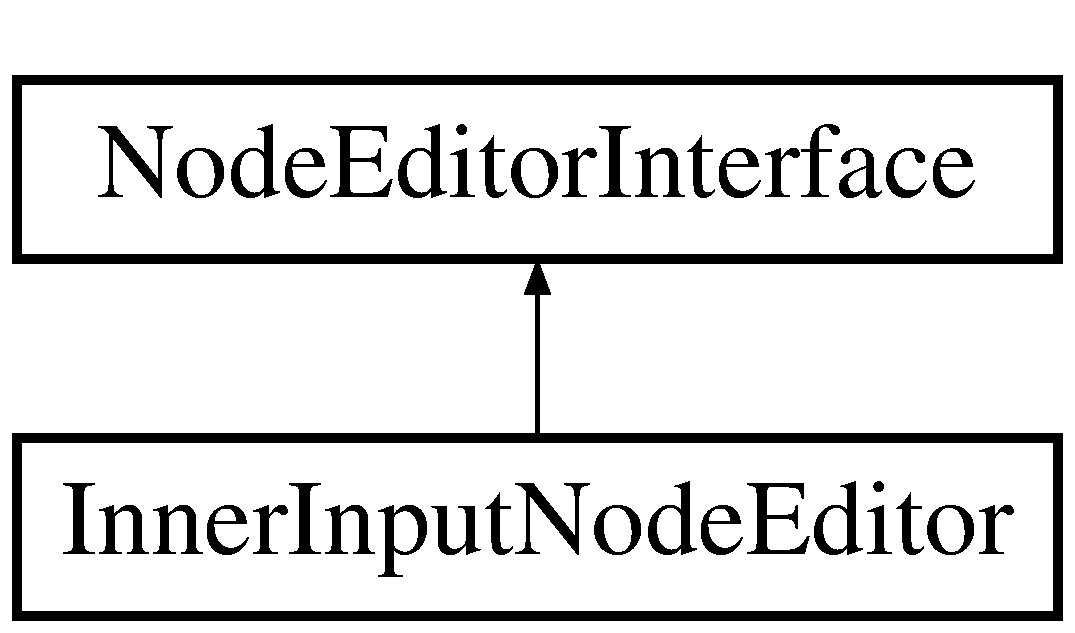
\includegraphics[height=2.000000cm]{class_inner_input_node_editor}
\end{center}
\end{figure}
\subsection*{Public Member Functions}
\begin{DoxyCompactItemize}
\item 
\mbox{\hyperlink{class_inner_input_node_editor_a08ef44059b09a0166808936d4f9aa5a9}{Inner\+Input\+Node\+Editor}} (\mbox{\hyperlink{class_inner_input_node}{Inner\+Input\+Node}} node, \mbox{\hyperlink{class_creature}{Creature}} parent\+Creature)
\item 
\mbox{\hyperlink{class_node}{Node}} \mbox{\hyperlink{class_inner_input_node_editor_a211d3bfaad897b853671c9c61366779f}{get\+Node}} ()
\item 
void \mbox{\hyperlink{class_inner_input_node_editor_ac3ad2c6210d5a95549d598b29e24caf0}{set\+Linked\+Node}} (string net\+Name, int out\+Layer\+Node\+Index, int net\+Layer)
\end{DoxyCompactItemize}


\subsection{Detailed Description}
A\+PI for Inner\+Input\+Nodes. 



\subsection{Constructor \& Destructor Documentation}
\mbox{\Hypertarget{class_inner_input_node_editor_a08ef44059b09a0166808936d4f9aa5a9}\label{class_inner_input_node_editor_a08ef44059b09a0166808936d4f9aa5a9}} 
\index{Inner\+Input\+Node\+Editor@{Inner\+Input\+Node\+Editor}!Inner\+Input\+Node\+Editor@{Inner\+Input\+Node\+Editor}}
\index{Inner\+Input\+Node\+Editor@{Inner\+Input\+Node\+Editor}!Inner\+Input\+Node\+Editor@{Inner\+Input\+Node\+Editor}}
\subsubsection{\texorpdfstring{Inner\+Input\+Node\+Editor()}{InnerInputNodeEditor()}}
{\footnotesize\ttfamily Inner\+Input\+Node\+Editor.\+Inner\+Input\+Node\+Editor (\begin{DoxyParamCaption}\item[{\mbox{\hyperlink{class_inner_input_node}{Inner\+Input\+Node}}}]{node,  }\item[{\mbox{\hyperlink{class_creature}{Creature}}}]{parent\+Creature }\end{DoxyParamCaption})}



\subsection{Member Function Documentation}
\mbox{\Hypertarget{class_inner_input_node_editor_a211d3bfaad897b853671c9c61366779f}\label{class_inner_input_node_editor_a211d3bfaad897b853671c9c61366779f}} 
\index{Inner\+Input\+Node\+Editor@{Inner\+Input\+Node\+Editor}!get\+Node@{get\+Node}}
\index{get\+Node@{get\+Node}!Inner\+Input\+Node\+Editor@{Inner\+Input\+Node\+Editor}}
\subsubsection{\texorpdfstring{get\+Node()}{getNode()}}
{\footnotesize\ttfamily \mbox{\hyperlink{class_node}{Node}} Inner\+Input\+Node\+Editor.\+get\+Node (\begin{DoxyParamCaption}{ }\end{DoxyParamCaption})}



Implements \mbox{\hyperlink{interface_node_editor_interface_a56e2abaedf17d7fbf2be90d521ec9363}{Node\+Editor\+Interface}}.

\mbox{\Hypertarget{class_inner_input_node_editor_ac3ad2c6210d5a95549d598b29e24caf0}\label{class_inner_input_node_editor_ac3ad2c6210d5a95549d598b29e24caf0}} 
\index{Inner\+Input\+Node\+Editor@{Inner\+Input\+Node\+Editor}!set\+Linked\+Node@{set\+Linked\+Node}}
\index{set\+Linked\+Node@{set\+Linked\+Node}!Inner\+Input\+Node\+Editor@{Inner\+Input\+Node\+Editor}}
\subsubsection{\texorpdfstring{set\+Linked\+Node()}{setLinkedNode()}}
{\footnotesize\ttfamily void Inner\+Input\+Node\+Editor.\+set\+Linked\+Node (\begin{DoxyParamCaption}\item[{string}]{net\+Name,  }\item[{int}]{out\+Layer\+Node\+Index,  }\item[{int}]{net\+Layer }\end{DoxyParamCaption})}



The documentation for this class was generated from the following file\+:\begin{DoxyCompactItemize}
\item 
\mbox{\hyperlink{_inner_input_node_editor_8cs}{Inner\+Input\+Node\+Editor.\+cs}}\end{DoxyCompactItemize}

\hypertarget{class_land}{}\section{Land Class Reference}
\label{class_land}\index{Land@{Land}}


Class for storing data about a location on the map. Also facilitates creature\textquotesingle{}s interaction with the environment.  


\subsection*{Public Member Functions}
\begin{DoxyCompactItemize}
\item 
bool \mbox{\hyperlink{class_land_ad66a06c6c305a42c12c5b63410242251}{creature\+Is\+On}} ()
\begin{DoxyCompactList}\small\item\em returns true if creature\+On is not null \end{DoxyCompactList}\item 
float \mbox{\hyperlink{class_land_ad2eefda30f5859bb62fc33804f445e20}{attempt\+Resource\+Consumption}} (string resource\+Key, float time\+Dedicated, float creature\+Ability, float c\+Storage\+Space)
\begin{DoxyCompactList}\small\item\em Try to consume resource of given name. \end{DoxyCompactList}\item 
\mbox{\hyperlink{class_land}{Land}} \mbox{\hyperlink{class_land_a39ae866c981982746dd04515bbab8238}{shallow\+Copy}} ()
\end{DoxyCompactItemize}
\subsection*{Public Attributes}
\begin{DoxyCompactItemize}
\item 
System.\+Collections.\+Generic.\+Dictionary$<$ string, \mbox{\hyperlink{class_resource_store}{Resource\+Store}} $>$ \mbox{\hyperlink{class_land_adcbc195ca2ec38fb30d0ef5e2fde4397}{property\+Dict}} = new Dictionary$<$string, \mbox{\hyperlink{class_resource_store}{Resource\+Store}}$>$()
\begin{DoxyCompactList}\small\item\em Stores resource values and other attributes of the land \end{DoxyCompactList}\item 
\mbox{\hyperlink{class_creature}{Creature}} \mbox{\hyperlink{class_land_a3cab3cf218bd21e41181b908bd76a053}{creature\+On}}
\begin{DoxyCompactList}\small\item\em Stores whatever creature is currently on this land. \end{DoxyCompactList}\item 
bool \mbox{\hyperlink{class_land_a309b7300b5d1bcdfec0fd7db41a94cc3}{is\+Dummy}} = false
\end{DoxyCompactItemize}


\subsection{Detailed Description}
Class for storing data about a location on the map. Also facilitates creature\textquotesingle{}s interaction with the environment. 



\subsection{Member Function Documentation}
\mbox{\Hypertarget{class_land_ad2eefda30f5859bb62fc33804f445e20}\label{class_land_ad2eefda30f5859bb62fc33804f445e20}} 
\index{Land@{Land}!attempt\+Resource\+Consumption@{attempt\+Resource\+Consumption}}
\index{attempt\+Resource\+Consumption@{attempt\+Resource\+Consumption}!Land@{Land}}
\subsubsection{\texorpdfstring{attempt\+Resource\+Consumption()}{attemptResourceConsumption()}}
{\footnotesize\ttfamily float Land.\+attempt\+Resource\+Consumption (\begin{DoxyParamCaption}\item[{string}]{resource\+Key,  }\item[{float}]{time\+Dedicated,  }\item[{float}]{creature\+Ability,  }\item[{float}]{c\+Storage\+Space }\end{DoxyParamCaption})}



Try to consume resource of given name. 


\begin{DoxyParams}{Parameters}
{\em resource\+Key} & Resource name.\\
\hline
{\em time\+Dedicated} & Comes from action time\+Cost variable.\\
\hline
\end{DoxyParams}
\mbox{\Hypertarget{class_land_ad66a06c6c305a42c12c5b63410242251}\label{class_land_ad66a06c6c305a42c12c5b63410242251}} 
\index{Land@{Land}!creature\+Is\+On@{creature\+Is\+On}}
\index{creature\+Is\+On@{creature\+Is\+On}!Land@{Land}}
\subsubsection{\texorpdfstring{creature\+Is\+On()}{creatureIsOn()}}
{\footnotesize\ttfamily bool Land.\+creature\+Is\+On (\begin{DoxyParamCaption}{ }\end{DoxyParamCaption})}



returns true if creature\+On is not null 

\mbox{\Hypertarget{class_land_a39ae866c981982746dd04515bbab8238}\label{class_land_a39ae866c981982746dd04515bbab8238}} 
\index{Land@{Land}!shallow\+Copy@{shallow\+Copy}}
\index{shallow\+Copy@{shallow\+Copy}!Land@{Land}}
\subsubsection{\texorpdfstring{shallow\+Copy()}{shallowCopy()}}
{\footnotesize\ttfamily \mbox{\hyperlink{class_land}{Land}} Land.\+shallow\+Copy (\begin{DoxyParamCaption}{ }\end{DoxyParamCaption})}



\subsection{Member Data Documentation}
\mbox{\Hypertarget{class_land_a3cab3cf218bd21e41181b908bd76a053}\label{class_land_a3cab3cf218bd21e41181b908bd76a053}} 
\index{Land@{Land}!creature\+On@{creature\+On}}
\index{creature\+On@{creature\+On}!Land@{Land}}
\subsubsection{\texorpdfstring{creature\+On}{creatureOn}}
{\footnotesize\ttfamily \mbox{\hyperlink{class_creature}{Creature}} Land.\+creature\+On}



Stores whatever creature is currently on this land. 

\mbox{\Hypertarget{class_land_a309b7300b5d1bcdfec0fd7db41a94cc3}\label{class_land_a309b7300b5d1bcdfec0fd7db41a94cc3}} 
\index{Land@{Land}!is\+Dummy@{is\+Dummy}}
\index{is\+Dummy@{is\+Dummy}!Land@{Land}}
\subsubsection{\texorpdfstring{is\+Dummy}{isDummy}}
{\footnotesize\ttfamily bool Land.\+is\+Dummy = false}

\mbox{\Hypertarget{class_land_adcbc195ca2ec38fb30d0ef5e2fde4397}\label{class_land_adcbc195ca2ec38fb30d0ef5e2fde4397}} 
\index{Land@{Land}!property\+Dict@{property\+Dict}}
\index{property\+Dict@{property\+Dict}!Land@{Land}}
\subsubsection{\texorpdfstring{property\+Dict}{propertyDict}}
{\footnotesize\ttfamily System.\+Collections.\+Generic.\+Dictionary$<$string, \mbox{\hyperlink{class_resource_store}{Resource\+Store}}$>$ Land.\+property\+Dict = new Dictionary$<$string, \mbox{\hyperlink{class_resource_store}{Resource\+Store}}$>$()}



Stores resource values and other attributes of the land 



The documentation for this class was generated from the following file\+:\begin{DoxyCompactItemize}
\item 
\mbox{\hyperlink{_land_8cs}{Land.\+cs}}\end{DoxyCompactItemize}

\hypertarget{class_land_resource_editor}{}\section{Land\+Resource\+Editor Class Reference}
\label{class_land_resource_editor}\index{Land\+Resource\+Editor@{Land\+Resource\+Editor}}


Used as interface for generating \mbox{\hyperlink{class_resource_store}{Resource\+Store}} objects.  


\subsection*{Public Member Functions}
\begin{DoxyCompactItemize}
\item 
\mbox{\hyperlink{class_land_resource_editor_ac8aacd2b8ec7329ec261665c0068f356}{Land\+Resource\+Editor}} (\mbox{\hyperlink{class_resource_store}{Resource\+Store}} \+\_\+resource\+Store)
\item 
void \mbox{\hyperlink{class_land_resource_editor_a5d3bfebc77d458924048d2ce42c25c55}{set\+Amt\+Consumed\+Per\+Time}} (float amount\+Consumed)
\begin{DoxyCompactList}\small\item\em Amount of the resource consumped per time unit. \end{DoxyCompactList}\item 
void \mbox{\hyperlink{class_land_resource_editor_a78ac1e33157301f579816da8fe86b8a1}{set\+Renewal\+Amt}} (float amount\+Renewed)
\begin{DoxyCompactList}\small\item\em Set how much the resource increases at the end of each interval number of turns (default interval is 10 turns) \end{DoxyCompactList}\item 
void \mbox{\hyperlink{class_land_resource_editor_a5390ac74d63e553c155fd515a6a035e0}{set\+Amount\+Of\+Resource}} (float amount)
\begin{DoxyCompactList}\small\item\em Set amount being stored \end{DoxyCompactList}\item 
void \mbox{\hyperlink{class_land_resource_editor_a2b401ce42af2c51063542978f500ccc1}{set\+Proportion\+Extracted}} (float proportion)
\begin{DoxyCompactList}\small\item\em Sets fraction of resource consumed per time unit that the creature actually recieves if creature does not have an ability for this. \end{DoxyCompactList}\item 
void \mbox{\hyperlink{class_land_resource_editor_a7f7cf4e6c7dacb9028a155dae2428e71}{set\+Max\+Amt}} (float max\+Amount)
\begin{DoxyCompactList}\small\item\em Sets maximum amount of the resource that can be stored. \end{DoxyCompactList}\end{DoxyCompactItemize}
\subsection*{Public Attributes}
\begin{DoxyCompactItemize}
\item 
\mbox{\hyperlink{class_resource_store}{Resource\+Store}} \mbox{\hyperlink{class_land_resource_editor_a5cde04313d283beee5f340a056b75bc2}{resource\+Store}}
\end{DoxyCompactItemize}


\subsection{Detailed Description}
Used as interface for generating \mbox{\hyperlink{class_resource_store}{Resource\+Store}} objects. 



\subsection{Constructor \& Destructor Documentation}
\mbox{\Hypertarget{class_land_resource_editor_ac8aacd2b8ec7329ec261665c0068f356}\label{class_land_resource_editor_ac8aacd2b8ec7329ec261665c0068f356}} 
\index{Land\+Resource\+Editor@{Land\+Resource\+Editor}!Land\+Resource\+Editor@{Land\+Resource\+Editor}}
\index{Land\+Resource\+Editor@{Land\+Resource\+Editor}!Land\+Resource\+Editor@{Land\+Resource\+Editor}}
\subsubsection{\texorpdfstring{Land\+Resource\+Editor()}{LandResourceEditor()}}
{\footnotesize\ttfamily Land\+Resource\+Editor.\+Land\+Resource\+Editor (\begin{DoxyParamCaption}\item[{\mbox{\hyperlink{class_resource_store}{Resource\+Store}}}]{\+\_\+resource\+Store }\end{DoxyParamCaption})}



\subsection{Member Function Documentation}
\mbox{\Hypertarget{class_land_resource_editor_a5390ac74d63e553c155fd515a6a035e0}\label{class_land_resource_editor_a5390ac74d63e553c155fd515a6a035e0}} 
\index{Land\+Resource\+Editor@{Land\+Resource\+Editor}!set\+Amount\+Of\+Resource@{set\+Amount\+Of\+Resource}}
\index{set\+Amount\+Of\+Resource@{set\+Amount\+Of\+Resource}!Land\+Resource\+Editor@{Land\+Resource\+Editor}}
\subsubsection{\texorpdfstring{set\+Amount\+Of\+Resource()}{setAmountOfResource()}}
{\footnotesize\ttfamily void Land\+Resource\+Editor.\+set\+Amount\+Of\+Resource (\begin{DoxyParamCaption}\item[{float}]{amount }\end{DoxyParamCaption})}



Set amount being stored 

\mbox{\Hypertarget{class_land_resource_editor_a5d3bfebc77d458924048d2ce42c25c55}\label{class_land_resource_editor_a5d3bfebc77d458924048d2ce42c25c55}} 
\index{Land\+Resource\+Editor@{Land\+Resource\+Editor}!set\+Amt\+Consumed\+Per\+Time@{set\+Amt\+Consumed\+Per\+Time}}
\index{set\+Amt\+Consumed\+Per\+Time@{set\+Amt\+Consumed\+Per\+Time}!Land\+Resource\+Editor@{Land\+Resource\+Editor}}
\subsubsection{\texorpdfstring{set\+Amt\+Consumed\+Per\+Time()}{setAmtConsumedPerTime()}}
{\footnotesize\ttfamily void Land\+Resource\+Editor.\+set\+Amt\+Consumed\+Per\+Time (\begin{DoxyParamCaption}\item[{float}]{amount\+Consumed }\end{DoxyParamCaption})}



Amount of the resource consumped per time unit. 

\mbox{\Hypertarget{class_land_resource_editor_a7f7cf4e6c7dacb9028a155dae2428e71}\label{class_land_resource_editor_a7f7cf4e6c7dacb9028a155dae2428e71}} 
\index{Land\+Resource\+Editor@{Land\+Resource\+Editor}!set\+Max\+Amt@{set\+Max\+Amt}}
\index{set\+Max\+Amt@{set\+Max\+Amt}!Land\+Resource\+Editor@{Land\+Resource\+Editor}}
\subsubsection{\texorpdfstring{set\+Max\+Amt()}{setMaxAmt()}}
{\footnotesize\ttfamily void Land\+Resource\+Editor.\+set\+Max\+Amt (\begin{DoxyParamCaption}\item[{float}]{max\+Amount }\end{DoxyParamCaption})}



Sets maximum amount of the resource that can be stored. 

\mbox{\Hypertarget{class_land_resource_editor_a2b401ce42af2c51063542978f500ccc1}\label{class_land_resource_editor_a2b401ce42af2c51063542978f500ccc1}} 
\index{Land\+Resource\+Editor@{Land\+Resource\+Editor}!set\+Proportion\+Extracted@{set\+Proportion\+Extracted}}
\index{set\+Proportion\+Extracted@{set\+Proportion\+Extracted}!Land\+Resource\+Editor@{Land\+Resource\+Editor}}
\subsubsection{\texorpdfstring{set\+Proportion\+Extracted()}{setProportionExtracted()}}
{\footnotesize\ttfamily void Land\+Resource\+Editor.\+set\+Proportion\+Extracted (\begin{DoxyParamCaption}\item[{float}]{proportion }\end{DoxyParamCaption})}



Sets fraction of resource consumed per time unit that the creature actually recieves if creature does not have an ability for this. 


\begin{DoxyParams}{Parameters}
{\em proportion} & Must be between 0 and 1.\\
\hline
\end{DoxyParams}
\mbox{\Hypertarget{class_land_resource_editor_a78ac1e33157301f579816da8fe86b8a1}\label{class_land_resource_editor_a78ac1e33157301f579816da8fe86b8a1}} 
\index{Land\+Resource\+Editor@{Land\+Resource\+Editor}!set\+Renewal\+Amt@{set\+Renewal\+Amt}}
\index{set\+Renewal\+Amt@{set\+Renewal\+Amt}!Land\+Resource\+Editor@{Land\+Resource\+Editor}}
\subsubsection{\texorpdfstring{set\+Renewal\+Amt()}{setRenewalAmt()}}
{\footnotesize\ttfamily void Land\+Resource\+Editor.\+set\+Renewal\+Amt (\begin{DoxyParamCaption}\item[{float}]{amount\+Renewed }\end{DoxyParamCaption})}



Set how much the resource increases at the end of each interval number of turns (default interval is 10 turns) 



\subsection{Member Data Documentation}
\mbox{\Hypertarget{class_land_resource_editor_a5cde04313d283beee5f340a056b75bc2}\label{class_land_resource_editor_a5cde04313d283beee5f340a056b75bc2}} 
\index{Land\+Resource\+Editor@{Land\+Resource\+Editor}!resource\+Store@{resource\+Store}}
\index{resource\+Store@{resource\+Store}!Land\+Resource\+Editor@{Land\+Resource\+Editor}}
\subsubsection{\texorpdfstring{resource\+Store}{resourceStore}}
{\footnotesize\ttfamily \mbox{\hyperlink{class_resource_store}{Resource\+Store}} Land\+Resource\+Editor.\+resource\+Store}



The documentation for this class was generated from the following file\+:\begin{DoxyCompactItemize}
\item 
\mbox{\hyperlink{_land_resource_editor_8cs}{Land\+Resource\+Editor.\+cs}}\end{DoxyCompactItemize}

\hypertarget{class_logistic_activ_behavior}{}\section{Logistic\+Activ\+Behavior Class Reference}
\label{class_logistic_activ_behavior}\index{Logistic\+Activ\+Behavior@{Logistic\+Activ\+Behavior}}


Implements logistic activation function.  


Inheritance diagram for Logistic\+Activ\+Behavior\+:\begin{figure}[H]
\begin{center}
\leavevmode
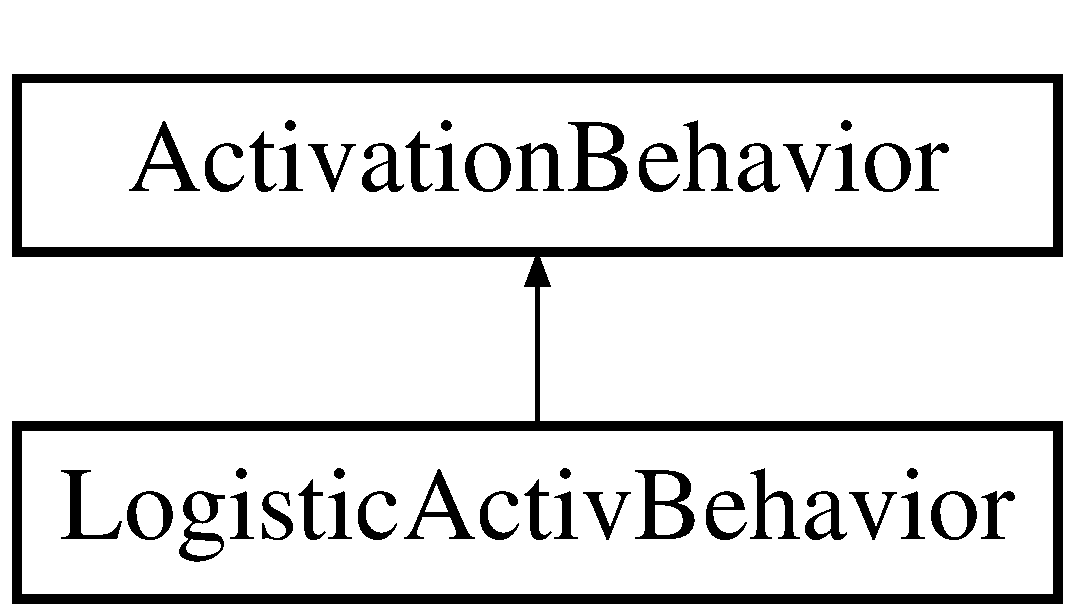
\includegraphics[height=2.000000cm]{class_logistic_activ_behavior}
\end{center}
\end{figure}
\subsection*{Public Member Functions}
\begin{DoxyCompactItemize}
\item 
float \mbox{\hyperlink{class_logistic_activ_behavior_a20a20f3e29d8aad19f35067a9304ee96}{activ\+Funct}} (float input)
\end{DoxyCompactItemize}


\subsection{Detailed Description}
Implements logistic activation function. 



\subsection{Member Function Documentation}
\mbox{\Hypertarget{class_logistic_activ_behavior_a20a20f3e29d8aad19f35067a9304ee96}\label{class_logistic_activ_behavior_a20a20f3e29d8aad19f35067a9304ee96}} 
\index{Logistic\+Activ\+Behavior@{Logistic\+Activ\+Behavior}!activ\+Funct@{activ\+Funct}}
\index{activ\+Funct@{activ\+Funct}!Logistic\+Activ\+Behavior@{Logistic\+Activ\+Behavior}}
\subsubsection{\texorpdfstring{activ\+Funct()}{activFunct()}}
{\footnotesize\ttfamily float Logistic\+Activ\+Behavior.\+activ\+Funct (\begin{DoxyParamCaption}\item[{float}]{input }\end{DoxyParamCaption})}



Implements \mbox{\hyperlink{interface_activation_behavior_a6c7af51cf1b10eaadcbf086231e5539b}{Activation\+Behavior}}.



The documentation for this class was generated from the following file\+:\begin{DoxyCompactItemize}
\item 
\mbox{\hyperlink{_logistic_activ_behavior_8cs}{Logistic\+Activ\+Behavior.\+cs}}\end{DoxyCompactItemize}

\hypertarget{class_logistic_with_neg_activ_behav}{}\section{Logistic\+With\+Neg\+Activ\+Behav Class Reference}
\label{class_logistic_with_neg_activ_behav}\index{Logistic\+With\+Neg\+Activ\+Behav@{Logistic\+With\+Neg\+Activ\+Behav}}


Logistic activation function, but mapped to \mbox{[}-\/1,1\mbox{]}  


Inheritance diagram for Logistic\+With\+Neg\+Activ\+Behav\+:\begin{figure}[H]
\begin{center}
\leavevmode
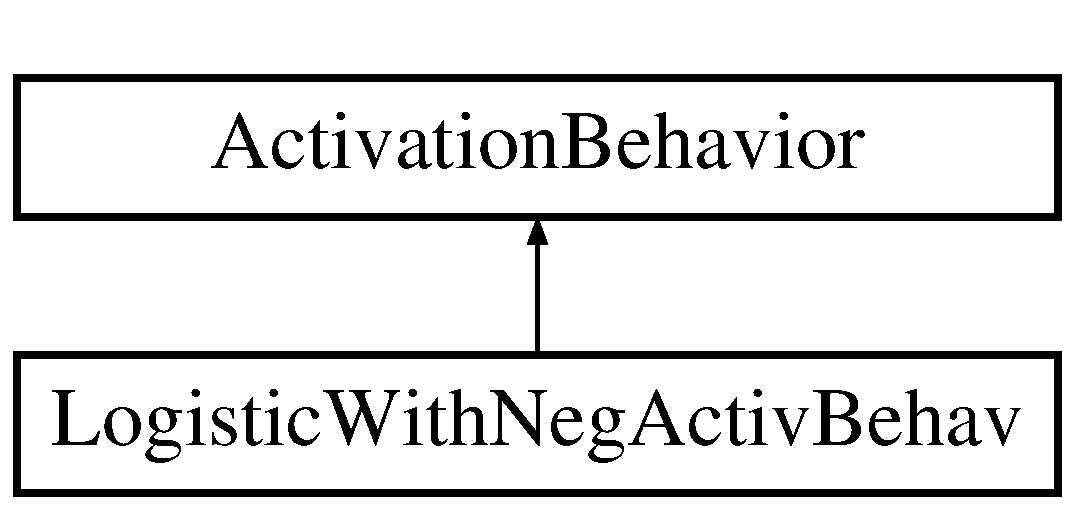
\includegraphics[height=2.000000cm]{class_logistic_with_neg_activ_behav}
\end{center}
\end{figure}
\subsection*{Public Member Functions}
\begin{DoxyCompactItemize}
\item 
float \mbox{\hyperlink{class_logistic_with_neg_activ_behav_abfe284e0e1854e171412cb2e6f0ad8e3}{activ\+Funct}} (float input)
\end{DoxyCompactItemize}


\subsection{Detailed Description}
Logistic activation function, but mapped to \mbox{[}-\/1,1\mbox{]} 



\subsection{Member Function Documentation}
\mbox{\Hypertarget{class_logistic_with_neg_activ_behav_abfe284e0e1854e171412cb2e6f0ad8e3}\label{class_logistic_with_neg_activ_behav_abfe284e0e1854e171412cb2e6f0ad8e3}} 
\index{Logistic\+With\+Neg\+Activ\+Behav@{Logistic\+With\+Neg\+Activ\+Behav}!activ\+Funct@{activ\+Funct}}
\index{activ\+Funct@{activ\+Funct}!Logistic\+With\+Neg\+Activ\+Behav@{Logistic\+With\+Neg\+Activ\+Behav}}
\subsubsection{\texorpdfstring{activ\+Funct()}{activFunct()}}
{\footnotesize\ttfamily float Logistic\+With\+Neg\+Activ\+Behav.\+activ\+Funct (\begin{DoxyParamCaption}\item[{float}]{input }\end{DoxyParamCaption})}



Implements \mbox{\hyperlink{interface_activation_behavior_a6c7af51cf1b10eaadcbf086231e5539b}{Activation\+Behavior}}.



The documentation for this class was generated from the following file\+:\begin{DoxyCompactItemize}
\item 
\mbox{\hyperlink{_logistic_with_neg_activ_behav_8cs}{Logistic\+With\+Neg\+Activ\+Behav.\+cs}}\end{DoxyCompactItemize}

\hypertarget{class_l_r_menu_behav}{}\section{L\+R\+Menu\+Behav Class Reference}
\label{class_l_r_menu_behav}\index{L\+R\+Menu\+Behav@{L\+R\+Menu\+Behav}}
Inheritance diagram for L\+R\+Menu\+Behav\+:\begin{figure}[H]
\begin{center}
\leavevmode
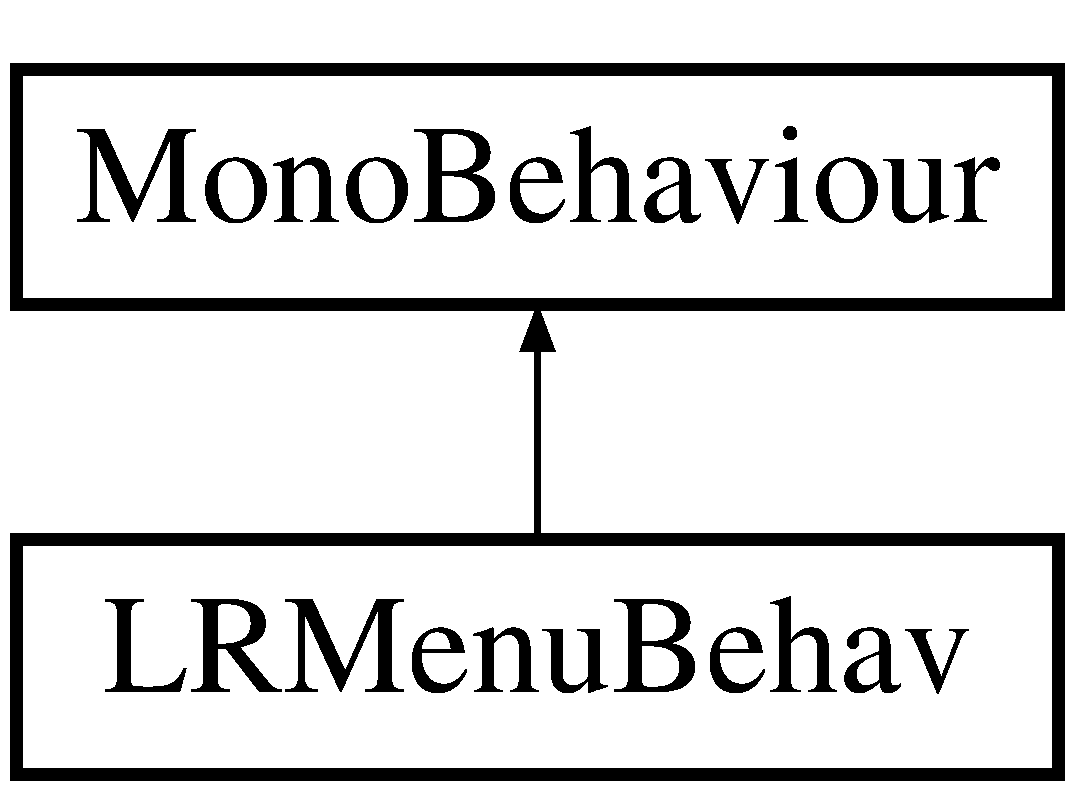
\includegraphics[height=2.000000cm]{class_l_r_menu_behav}
\end{center}
\end{figure}
\subsection*{Public Member Functions}
\begin{DoxyCompactItemize}
\item 
void \mbox{\hyperlink{class_l_r_menu_behav_afac347dc845bbc5907d7f113a5ab83a6}{load\+Land\+Res\+Menu}} (\mbox{\hyperlink{class_ecosystem_editor}{Ecosystem\+Editor}} ee)
\begin{DoxyCompactList}\small\item\em load the creature editor menu using the ecosystem editor \end{DoxyCompactList}\item 
void \mbox{\hyperlink{class_l_r_menu_behav_ae018bba40d93916f0b390dff34071506}{save\+Settings}} ()
\begin{DoxyCompactList}\small\item\em saves all information that the user entered into the menu \end{DoxyCompactList}\end{DoxyCompactItemize}
\subsection*{Public Attributes}
\begin{DoxyCompactItemize}
\item 
\mbox{\hyperlink{class_land_resource_editor}{Land\+Resource\+Editor}} \mbox{\hyperlink{class_l_r_menu_behav_a3433b21bf4da825d03191d3df7bccea4}{lr\+Editor}}
\item 
Game\+Object \mbox{\hyperlink{class_l_r_menu_behav_a8885c84d3b95c8275b8316b1268172a2}{u\+I\+Parent}}
\item 
Game\+Object \mbox{\hyperlink{class_l_r_menu_behav_abf503e806d61c19a2e4e2b18f47f734f}{error\+Obj}}
\item 
Game\+Object \mbox{\hyperlink{class_l_r_menu_behav_a36fe40f9fe549ef8bf734e961d580026}{amt\+Stored\+Text}}
\item 
Game\+Object \mbox{\hyperlink{class_l_r_menu_behav_ad95cf2a9f97147c12205e6f06ecdd8d7}{max\+Amt\+Text}}
\item 
Game\+Object \mbox{\hyperlink{class_l_r_menu_behav_af3e6af9c5f7527c8c13167303e7cacc9}{renew\+Amt\+Text}}
\item 
Game\+Object \mbox{\hyperlink{class_l_r_menu_behav_afab64deacaeb870162a7084e3b7ee103}{amt\+Cons\+Text}}
\item 
Game\+Object \mbox{\hyperlink{class_l_r_menu_behav_a99dafb63ae87a4b82fb89b681605849c}{res\+Name\+Text}}
\item 
Game\+Object \mbox{\hyperlink{class_l_r_menu_behav_abc2c0ca0f972e72c3d0a7950a8865783}{prop\+Extract\+Text}}
\end{DoxyCompactItemize}


\subsection{Member Function Documentation}
\mbox{\Hypertarget{class_l_r_menu_behav_afac347dc845bbc5907d7f113a5ab83a6}\label{class_l_r_menu_behav_afac347dc845bbc5907d7f113a5ab83a6}} 
\index{L\+R\+Menu\+Behav@{L\+R\+Menu\+Behav}!load\+Land\+Res\+Menu@{load\+Land\+Res\+Menu}}
\index{load\+Land\+Res\+Menu@{load\+Land\+Res\+Menu}!L\+R\+Menu\+Behav@{L\+R\+Menu\+Behav}}
\subsubsection{\texorpdfstring{load\+Land\+Res\+Menu()}{loadLandResMenu()}}
{\footnotesize\ttfamily void L\+R\+Menu\+Behav.\+load\+Land\+Res\+Menu (\begin{DoxyParamCaption}\item[{\mbox{\hyperlink{class_ecosystem_editor}{Ecosystem\+Editor}}}]{ee }\end{DoxyParamCaption})}



load the creature editor menu using the ecosystem editor 

\mbox{\Hypertarget{class_l_r_menu_behav_ae018bba40d93916f0b390dff34071506}\label{class_l_r_menu_behav_ae018bba40d93916f0b390dff34071506}} 
\index{L\+R\+Menu\+Behav@{L\+R\+Menu\+Behav}!save\+Settings@{save\+Settings}}
\index{save\+Settings@{save\+Settings}!L\+R\+Menu\+Behav@{L\+R\+Menu\+Behav}}
\subsubsection{\texorpdfstring{save\+Settings()}{saveSettings()}}
{\footnotesize\ttfamily void L\+R\+Menu\+Behav.\+save\+Settings (\begin{DoxyParamCaption}{ }\end{DoxyParamCaption})}



saves all information that the user entered into the menu 



\subsection{Member Data Documentation}
\mbox{\Hypertarget{class_l_r_menu_behav_afab64deacaeb870162a7084e3b7ee103}\label{class_l_r_menu_behav_afab64deacaeb870162a7084e3b7ee103}} 
\index{L\+R\+Menu\+Behav@{L\+R\+Menu\+Behav}!amt\+Cons\+Text@{amt\+Cons\+Text}}
\index{amt\+Cons\+Text@{amt\+Cons\+Text}!L\+R\+Menu\+Behav@{L\+R\+Menu\+Behav}}
\subsubsection{\texorpdfstring{amt\+Cons\+Text}{amtConsText}}
{\footnotesize\ttfamily Game\+Object L\+R\+Menu\+Behav.\+amt\+Cons\+Text}

\mbox{\Hypertarget{class_l_r_menu_behav_a36fe40f9fe549ef8bf734e961d580026}\label{class_l_r_menu_behav_a36fe40f9fe549ef8bf734e961d580026}} 
\index{L\+R\+Menu\+Behav@{L\+R\+Menu\+Behav}!amt\+Stored\+Text@{amt\+Stored\+Text}}
\index{amt\+Stored\+Text@{amt\+Stored\+Text}!L\+R\+Menu\+Behav@{L\+R\+Menu\+Behav}}
\subsubsection{\texorpdfstring{amt\+Stored\+Text}{amtStoredText}}
{\footnotesize\ttfamily Game\+Object L\+R\+Menu\+Behav.\+amt\+Stored\+Text}

\mbox{\Hypertarget{class_l_r_menu_behav_abf503e806d61c19a2e4e2b18f47f734f}\label{class_l_r_menu_behav_abf503e806d61c19a2e4e2b18f47f734f}} 
\index{L\+R\+Menu\+Behav@{L\+R\+Menu\+Behav}!error\+Obj@{error\+Obj}}
\index{error\+Obj@{error\+Obj}!L\+R\+Menu\+Behav@{L\+R\+Menu\+Behav}}
\subsubsection{\texorpdfstring{error\+Obj}{errorObj}}
{\footnotesize\ttfamily Game\+Object L\+R\+Menu\+Behav.\+error\+Obj}

\mbox{\Hypertarget{class_l_r_menu_behav_a3433b21bf4da825d03191d3df7bccea4}\label{class_l_r_menu_behav_a3433b21bf4da825d03191d3df7bccea4}} 
\index{L\+R\+Menu\+Behav@{L\+R\+Menu\+Behav}!lr\+Editor@{lr\+Editor}}
\index{lr\+Editor@{lr\+Editor}!L\+R\+Menu\+Behav@{L\+R\+Menu\+Behav}}
\subsubsection{\texorpdfstring{lr\+Editor}{lrEditor}}
{\footnotesize\ttfamily \mbox{\hyperlink{class_land_resource_editor}{Land\+Resource\+Editor}} L\+R\+Menu\+Behav.\+lr\+Editor}

\mbox{\Hypertarget{class_l_r_menu_behav_ad95cf2a9f97147c12205e6f06ecdd8d7}\label{class_l_r_menu_behav_ad95cf2a9f97147c12205e6f06ecdd8d7}} 
\index{L\+R\+Menu\+Behav@{L\+R\+Menu\+Behav}!max\+Amt\+Text@{max\+Amt\+Text}}
\index{max\+Amt\+Text@{max\+Amt\+Text}!L\+R\+Menu\+Behav@{L\+R\+Menu\+Behav}}
\subsubsection{\texorpdfstring{max\+Amt\+Text}{maxAmtText}}
{\footnotesize\ttfamily Game\+Object L\+R\+Menu\+Behav.\+max\+Amt\+Text}

\mbox{\Hypertarget{class_l_r_menu_behav_abc2c0ca0f972e72c3d0a7950a8865783}\label{class_l_r_menu_behav_abc2c0ca0f972e72c3d0a7950a8865783}} 
\index{L\+R\+Menu\+Behav@{L\+R\+Menu\+Behav}!prop\+Extract\+Text@{prop\+Extract\+Text}}
\index{prop\+Extract\+Text@{prop\+Extract\+Text}!L\+R\+Menu\+Behav@{L\+R\+Menu\+Behav}}
\subsubsection{\texorpdfstring{prop\+Extract\+Text}{propExtractText}}
{\footnotesize\ttfamily Game\+Object L\+R\+Menu\+Behav.\+prop\+Extract\+Text}

\mbox{\Hypertarget{class_l_r_menu_behav_af3e6af9c5f7527c8c13167303e7cacc9}\label{class_l_r_menu_behav_af3e6af9c5f7527c8c13167303e7cacc9}} 
\index{L\+R\+Menu\+Behav@{L\+R\+Menu\+Behav}!renew\+Amt\+Text@{renew\+Amt\+Text}}
\index{renew\+Amt\+Text@{renew\+Amt\+Text}!L\+R\+Menu\+Behav@{L\+R\+Menu\+Behav}}
\subsubsection{\texorpdfstring{renew\+Amt\+Text}{renewAmtText}}
{\footnotesize\ttfamily Game\+Object L\+R\+Menu\+Behav.\+renew\+Amt\+Text}

\mbox{\Hypertarget{class_l_r_menu_behav_a99dafb63ae87a4b82fb89b681605849c}\label{class_l_r_menu_behav_a99dafb63ae87a4b82fb89b681605849c}} 
\index{L\+R\+Menu\+Behav@{L\+R\+Menu\+Behav}!res\+Name\+Text@{res\+Name\+Text}}
\index{res\+Name\+Text@{res\+Name\+Text}!L\+R\+Menu\+Behav@{L\+R\+Menu\+Behav}}
\subsubsection{\texorpdfstring{res\+Name\+Text}{resNameText}}
{\footnotesize\ttfamily Game\+Object L\+R\+Menu\+Behav.\+res\+Name\+Text}

\mbox{\Hypertarget{class_l_r_menu_behav_a8885c84d3b95c8275b8316b1268172a2}\label{class_l_r_menu_behav_a8885c84d3b95c8275b8316b1268172a2}} 
\index{L\+R\+Menu\+Behav@{L\+R\+Menu\+Behav}!u\+I\+Parent@{u\+I\+Parent}}
\index{u\+I\+Parent@{u\+I\+Parent}!L\+R\+Menu\+Behav@{L\+R\+Menu\+Behav}}
\subsubsection{\texorpdfstring{u\+I\+Parent}{uIParent}}
{\footnotesize\ttfamily Game\+Object L\+R\+Menu\+Behav.\+u\+I\+Parent}



The documentation for this class was generated from the following file\+:\begin{DoxyCompactItemize}
\item 
\mbox{\hyperlink{_l_r_menu_behav_8cs}{L\+R\+Menu\+Behav.\+cs}}\end{DoxyCompactItemize}

\hypertarget{class_main_menu_behav}{}\section{Main\+Menu\+Behav Class Reference}
\label{class_main_menu_behav}\index{Main\+Menu\+Behav@{Main\+Menu\+Behav}}
Inheritance diagram for Main\+Menu\+Behav\+:\begin{figure}[H]
\begin{center}
\leavevmode
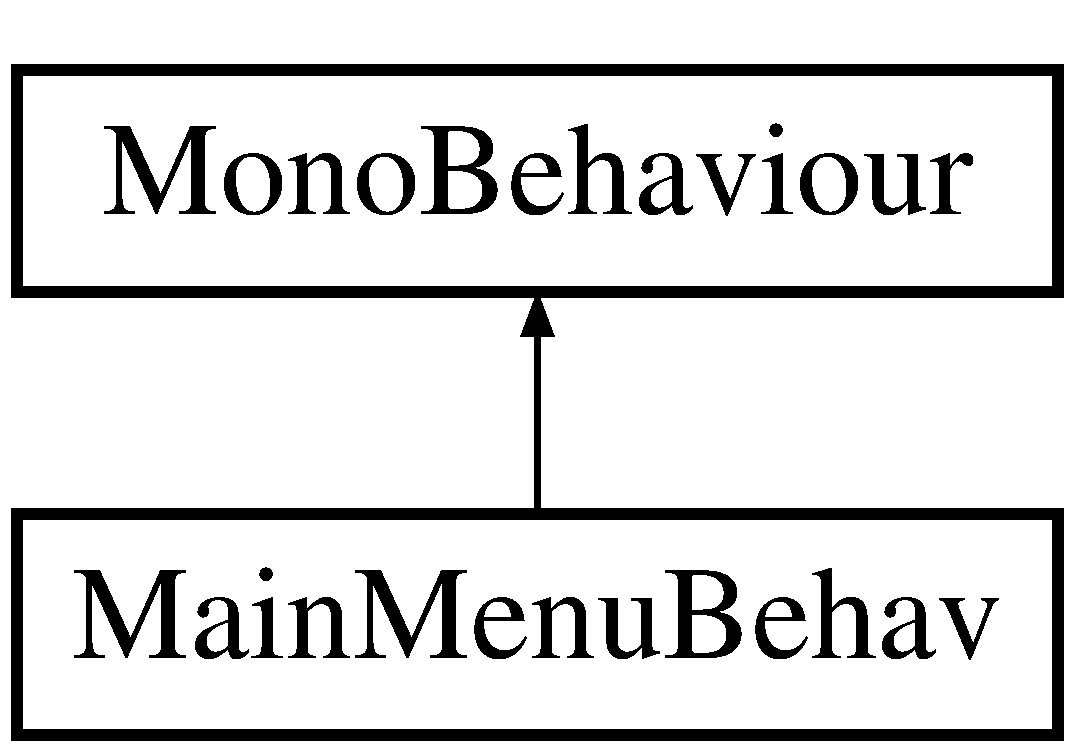
\includegraphics[height=2.000000cm]{class_main_menu_behav}
\end{center}
\end{figure}
\subsection*{Public Member Functions}
\begin{DoxyCompactItemize}
\item 
void \mbox{\hyperlink{class_main_menu_behav_ae23e7f61fb7c6affea630307fac58f92}{create\+New\+Ecosystem}} ()
\begin{DoxyCompactList}\small\item\em provides the ecosystem menu with a new ecosystem to edit \end{DoxyCompactList}\item 
void \mbox{\hyperlink{class_main_menu_behav_ac17fe569792552206ddae7d65d66ced3}{save\+Current\+Ecosystem}} ()
\begin{DoxyCompactList}\small\item\em saves last ecosystem edited by ecosystem menu to the ecosystem dictionary \end{DoxyCompactList}\item 
void \mbox{\hyperlink{class_main_menu_behav_a9d999e202894ebe1df82a88e677cc45e}{start\+Simulation}} ()
\end{DoxyCompactItemize}
\subsection*{Public Attributes}
\begin{DoxyCompactItemize}
\item 
Game\+Object \mbox{\hyperlink{class_main_menu_behav_a74da9f8edb36612d2587f00006db89e8}{u\+I\+Parent}}
\item 
Game\+Object \mbox{\hyperlink{class_main_menu_behav_af762eecb3eeea9808e64e35758efdca9}{eco\+Menu}}
\item 
int \mbox{\hyperlink{class_main_menu_behav_a6b087cc95f494547d1f0e04a5c045531}{sim\+Steps}}
\end{DoxyCompactItemize}


\subsection{Member Function Documentation}
\mbox{\Hypertarget{class_main_menu_behav_ae23e7f61fb7c6affea630307fac58f92}\label{class_main_menu_behav_ae23e7f61fb7c6affea630307fac58f92}} 
\index{Main\+Menu\+Behav@{Main\+Menu\+Behav}!create\+New\+Ecosystem@{create\+New\+Ecosystem}}
\index{create\+New\+Ecosystem@{create\+New\+Ecosystem}!Main\+Menu\+Behav@{Main\+Menu\+Behav}}
\subsubsection{\texorpdfstring{create\+New\+Ecosystem()}{createNewEcosystem()}}
{\footnotesize\ttfamily void Main\+Menu\+Behav.\+create\+New\+Ecosystem (\begin{DoxyParamCaption}{ }\end{DoxyParamCaption})}



provides the ecosystem menu with a new ecosystem to edit 

\mbox{\Hypertarget{class_main_menu_behav_ac17fe569792552206ddae7d65d66ced3}\label{class_main_menu_behav_ac17fe569792552206ddae7d65d66ced3}} 
\index{Main\+Menu\+Behav@{Main\+Menu\+Behav}!save\+Current\+Ecosystem@{save\+Current\+Ecosystem}}
\index{save\+Current\+Ecosystem@{save\+Current\+Ecosystem}!Main\+Menu\+Behav@{Main\+Menu\+Behav}}
\subsubsection{\texorpdfstring{save\+Current\+Ecosystem()}{saveCurrentEcosystem()}}
{\footnotesize\ttfamily void Main\+Menu\+Behav.\+save\+Current\+Ecosystem (\begin{DoxyParamCaption}{ }\end{DoxyParamCaption})}



saves last ecosystem edited by ecosystem menu to the ecosystem dictionary 

\mbox{\Hypertarget{class_main_menu_behav_a9d999e202894ebe1df82a88e677cc45e}\label{class_main_menu_behav_a9d999e202894ebe1df82a88e677cc45e}} 
\index{Main\+Menu\+Behav@{Main\+Menu\+Behav}!start\+Simulation@{start\+Simulation}}
\index{start\+Simulation@{start\+Simulation}!Main\+Menu\+Behav@{Main\+Menu\+Behav}}
\subsubsection{\texorpdfstring{start\+Simulation()}{startSimulation()}}
{\footnotesize\ttfamily void Main\+Menu\+Behav.\+start\+Simulation (\begin{DoxyParamCaption}{ }\end{DoxyParamCaption})}



\subsection{Member Data Documentation}
\mbox{\Hypertarget{class_main_menu_behav_af762eecb3eeea9808e64e35758efdca9}\label{class_main_menu_behav_af762eecb3eeea9808e64e35758efdca9}} 
\index{Main\+Menu\+Behav@{Main\+Menu\+Behav}!eco\+Menu@{eco\+Menu}}
\index{eco\+Menu@{eco\+Menu}!Main\+Menu\+Behav@{Main\+Menu\+Behav}}
\subsubsection{\texorpdfstring{eco\+Menu}{ecoMenu}}
{\footnotesize\ttfamily Game\+Object Main\+Menu\+Behav.\+eco\+Menu}

\mbox{\Hypertarget{class_main_menu_behav_a6b087cc95f494547d1f0e04a5c045531}\label{class_main_menu_behav_a6b087cc95f494547d1f0e04a5c045531}} 
\index{Main\+Menu\+Behav@{Main\+Menu\+Behav}!sim\+Steps@{sim\+Steps}}
\index{sim\+Steps@{sim\+Steps}!Main\+Menu\+Behav@{Main\+Menu\+Behav}}
\subsubsection{\texorpdfstring{sim\+Steps}{simSteps}}
{\footnotesize\ttfamily int Main\+Menu\+Behav.\+sim\+Steps}

\mbox{\Hypertarget{class_main_menu_behav_a74da9f8edb36612d2587f00006db89e8}\label{class_main_menu_behav_a74da9f8edb36612d2587f00006db89e8}} 
\index{Main\+Menu\+Behav@{Main\+Menu\+Behav}!u\+I\+Parent@{u\+I\+Parent}}
\index{u\+I\+Parent@{u\+I\+Parent}!Main\+Menu\+Behav@{Main\+Menu\+Behav}}
\subsubsection{\texorpdfstring{u\+I\+Parent}{uIParent}}
{\footnotesize\ttfamily Game\+Object Main\+Menu\+Behav.\+u\+I\+Parent}



The documentation for this class was generated from the following file\+:\begin{DoxyCompactItemize}
\item 
\mbox{\hyperlink{_main_menu_behav_8cs}{Main\+Menu\+Behav.\+cs}}\end{DoxyCompactItemize}

\hypertarget{class_map_editor}{}\section{Map\+Editor Class Reference}
\label{class_map_editor}\index{Map\+Editor@{Map\+Editor}}


A\+PI for editing the map\+: a 2D array of \mbox{\hyperlink{class_land}{Land}} spaces. Used to generate the map, and add resources.  


\subsection*{Public Member Functions}
\begin{DoxyCompactItemize}
\item 
\mbox{\hyperlink{class_map_editor_acc8af16a98b138b39e1c0e8f3d3ad83b}{Map\+Editor}} (List$<$ List$<$ \mbox{\hyperlink{class_land}{Land}} $>$$>$ \+\_\+map, Dictionary$<$ string, \mbox{\hyperlink{class_resource_store}{Resource\+Store}} $>$ \+\_\+res\+Options)
\item 
void \mbox{\hyperlink{class_map_editor_af0faf8e47a1ed57ada0e1d1f56b64be4}{add\+Uniform\+Resource}} (string resource, float level)
\begin{DoxyCompactList}\small\item\em Adds resource uniformly to all lands on map. \end{DoxyCompactList}\item 
void \mbox{\hyperlink{class_map_editor_a3f0e4bacb89992b0aa0aaa4f17aafd28}{add\+L\+E\+R\+P\+X\+Resource}} (string resource, float max\+Amt)
\item 
void \mbox{\hyperlink{class_map_editor_a3da89d803fa558eb9cc071a604f4351c}{generate\+Map}} (int length, int width)
\end{DoxyCompactItemize}
\subsection*{Public Attributes}
\begin{DoxyCompactItemize}
\item 
List$<$ List$<$ \mbox{\hyperlink{class_land}{Land}} $>$ $>$ \mbox{\hyperlink{class_map_editor_a3899ec34c7e9acb6cd8b98434504e726}{map}}
\begin{DoxyCompactList}\small\item\em Map to be edited \end{DoxyCompactList}\end{DoxyCompactItemize}


\subsection{Detailed Description}
A\+PI for editing the map\+: a 2D array of \mbox{\hyperlink{class_land}{Land}} spaces. Used to generate the map, and add resources. 



\subsection{Constructor \& Destructor Documentation}
\mbox{\Hypertarget{class_map_editor_acc8af16a98b138b39e1c0e8f3d3ad83b}\label{class_map_editor_acc8af16a98b138b39e1c0e8f3d3ad83b}} 
\index{Map\+Editor@{Map\+Editor}!Map\+Editor@{Map\+Editor}}
\index{Map\+Editor@{Map\+Editor}!Map\+Editor@{Map\+Editor}}
\subsubsection{\texorpdfstring{Map\+Editor()}{MapEditor()}}
{\footnotesize\ttfamily Map\+Editor.\+Map\+Editor (\begin{DoxyParamCaption}\item[{List$<$ List$<$ \mbox{\hyperlink{class_land}{Land}} $>$$>$}]{\+\_\+map,  }\item[{Dictionary$<$ string, \mbox{\hyperlink{class_resource_store}{Resource\+Store}} $>$}]{\+\_\+res\+Options }\end{DoxyParamCaption})}



\subsection{Member Function Documentation}
\mbox{\Hypertarget{class_map_editor_a3f0e4bacb89992b0aa0aaa4f17aafd28}\label{class_map_editor_a3f0e4bacb89992b0aa0aaa4f17aafd28}} 
\index{Map\+Editor@{Map\+Editor}!add\+L\+E\+R\+P\+X\+Resource@{add\+L\+E\+R\+P\+X\+Resource}}
\index{add\+L\+E\+R\+P\+X\+Resource@{add\+L\+E\+R\+P\+X\+Resource}!Map\+Editor@{Map\+Editor}}
\subsubsection{\texorpdfstring{add\+L\+E\+R\+P\+X\+Resource()}{addLERPXResource()}}
{\footnotesize\ttfamily void Map\+Editor.\+add\+L\+E\+R\+P\+X\+Resource (\begin{DoxyParamCaption}\item[{string}]{resource,  }\item[{float}]{max\+Amt }\end{DoxyParamCaption})}

\mbox{\Hypertarget{class_map_editor_af0faf8e47a1ed57ada0e1d1f56b64be4}\label{class_map_editor_af0faf8e47a1ed57ada0e1d1f56b64be4}} 
\index{Map\+Editor@{Map\+Editor}!add\+Uniform\+Resource@{add\+Uniform\+Resource}}
\index{add\+Uniform\+Resource@{add\+Uniform\+Resource}!Map\+Editor@{Map\+Editor}}
\subsubsection{\texorpdfstring{add\+Uniform\+Resource()}{addUniformResource()}}
{\footnotesize\ttfamily void Map\+Editor.\+add\+Uniform\+Resource (\begin{DoxyParamCaption}\item[{string}]{resource,  }\item[{float}]{level }\end{DoxyParamCaption})}



Adds resource uniformly to all lands on map. 


\begin{DoxyParams}{Parameters}
{\em level} & Fraction of max possible amount of resource. Must be between 0 and 1.\\
\hline
\end{DoxyParams}
\mbox{\Hypertarget{class_map_editor_a3da89d803fa558eb9cc071a604f4351c}\label{class_map_editor_a3da89d803fa558eb9cc071a604f4351c}} 
\index{Map\+Editor@{Map\+Editor}!generate\+Map@{generate\+Map}}
\index{generate\+Map@{generate\+Map}!Map\+Editor@{Map\+Editor}}
\subsubsection{\texorpdfstring{generate\+Map()}{generateMap()}}
{\footnotesize\ttfamily void Map\+Editor.\+generate\+Map (\begin{DoxyParamCaption}\item[{int}]{length,  }\item[{int}]{width }\end{DoxyParamCaption})}



\subsection{Member Data Documentation}
\mbox{\Hypertarget{class_map_editor_a3899ec34c7e9acb6cd8b98434504e726}\label{class_map_editor_a3899ec34c7e9acb6cd8b98434504e726}} 
\index{Map\+Editor@{Map\+Editor}!map@{map}}
\index{map@{map}!Map\+Editor@{Map\+Editor}}
\subsubsection{\texorpdfstring{map}{map}}
{\footnotesize\ttfamily List$<$List$<$\mbox{\hyperlink{class_land}{Land}}$>$ $>$ Map\+Editor.\+map}



Map to be edited 



The documentation for this class was generated from the following file\+:\begin{DoxyCompactItemize}
\item 
\mbox{\hyperlink{_map_editor_8cs}{Map\+Editor.\+cs}}\end{DoxyCompactItemize}

\hypertarget{class_memory_input_node}{}\section{Memory\+Input\+Node Class Reference}
\label{class_memory_input_node}\index{Memory\+Input\+Node@{Memory\+Input\+Node}}
Inheritance diagram for Memory\+Input\+Node\+:\begin{figure}[H]
\begin{center}
\leavevmode
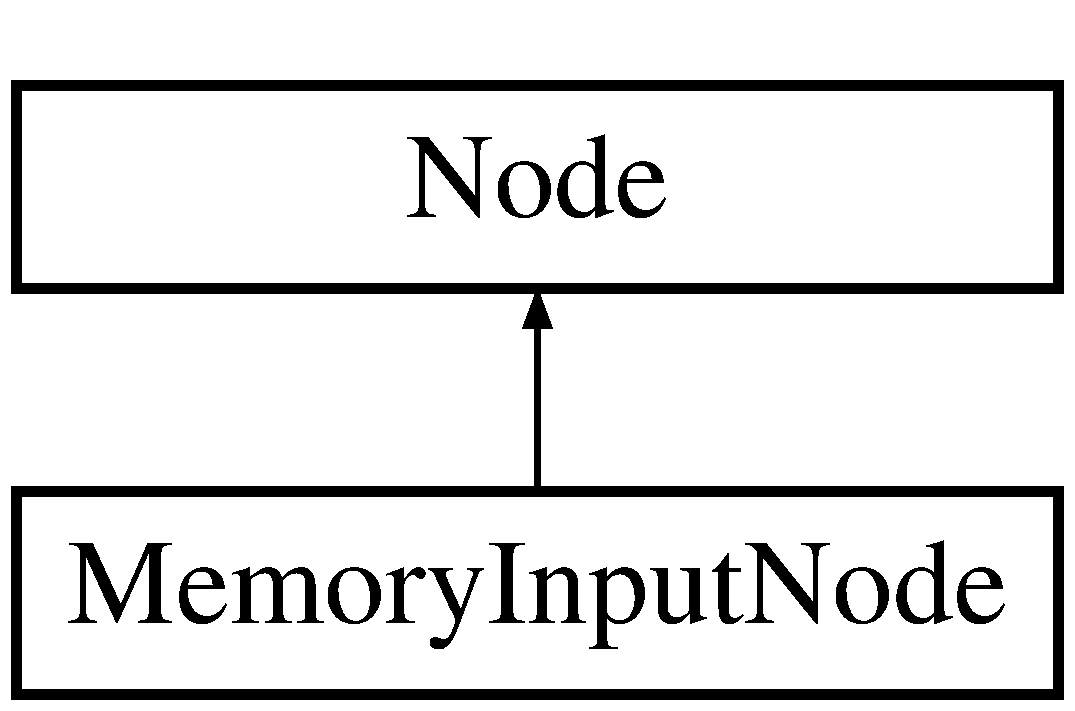
\includegraphics[height=2.000000cm]{class_memory_input_node}
\end{center}
\end{figure}
\subsection*{Public Member Functions}
\begin{DoxyCompactItemize}
\item 
override void \mbox{\hyperlink{class_memory_input_node_aa1efec4e8bc221a879c959ba9941587b}{update\+Value}} ()
\end{DoxyCompactItemize}
\subsection*{Additional Inherited Members}


\subsection{Member Function Documentation}
\mbox{\Hypertarget{class_memory_input_node_aa1efec4e8bc221a879c959ba9941587b}\label{class_memory_input_node_aa1efec4e8bc221a879c959ba9941587b}} 
\index{Memory\+Input\+Node@{Memory\+Input\+Node}!update\+Value@{update\+Value}}
\index{update\+Value@{update\+Value}!Memory\+Input\+Node@{Memory\+Input\+Node}}
\subsubsection{\texorpdfstring{update\+Value()}{updateValue()}}
{\footnotesize\ttfamily override void Memory\+Input\+Node.\+update\+Value (\begin{DoxyParamCaption}{ }\end{DoxyParamCaption})\hspace{0.3cm}{\ttfamily [virtual]}}







Implements \mbox{\hyperlink{class_node_a85ebd0e36c25430570b94f923afd2a62}{Node}}.



The documentation for this class was generated from the following file\+:\begin{DoxyCompactItemize}
\item 
\mbox{\hyperlink{_memory_input_node_8cs}{Memory\+Input\+Node.\+cs}}\end{DoxyCompactItemize}

\hypertarget{class_move_action}{}\section{Move\+Action Class Reference}
\label{class_move_action}\index{Move\+Action@{Move\+Action}}
Inheritance diagram for Move\+Action\+:\begin{figure}[H]
\begin{center}
\leavevmode
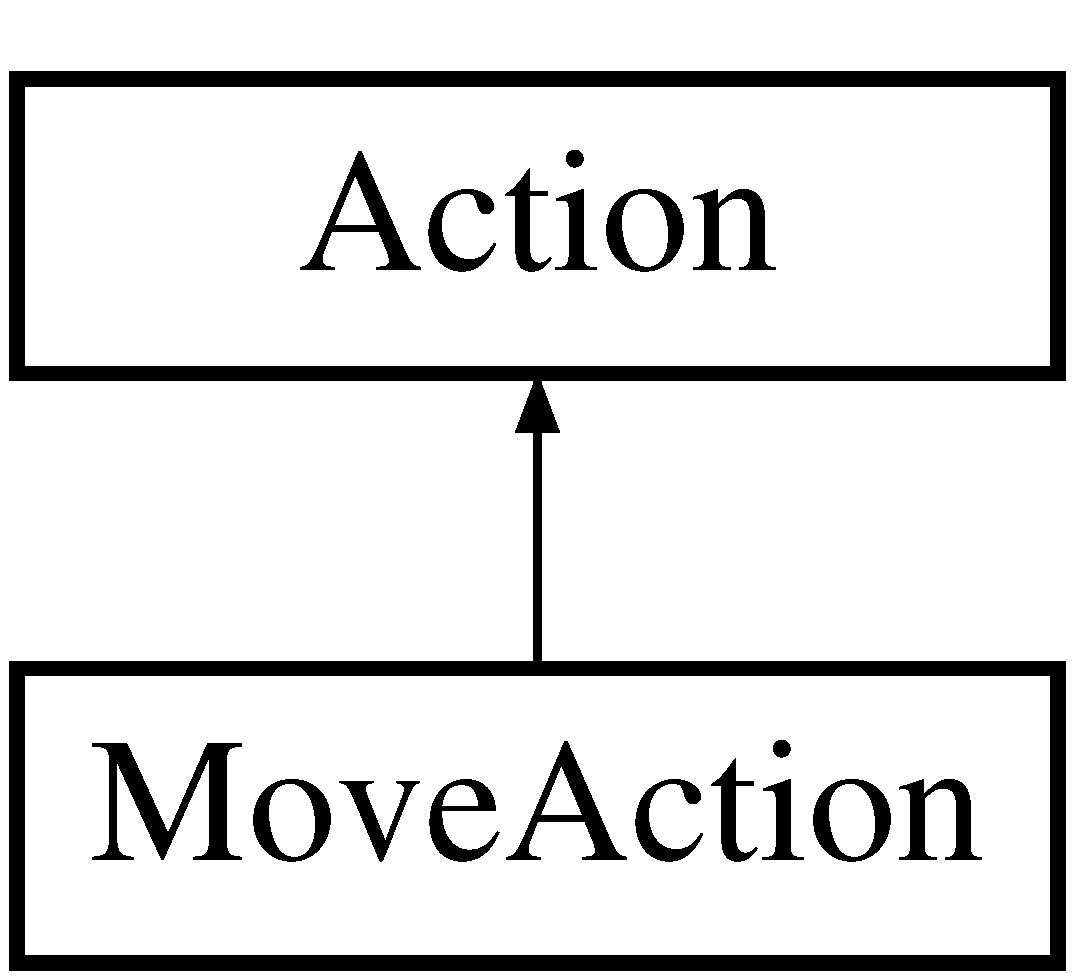
\includegraphics[height=2.000000cm]{class_move_action}
\end{center}
\end{figure}
\subsection*{Public Member Functions}
\begin{DoxyCompactItemize}
\item 
\mbox{\hyperlink{class_move_action_a163a34639a00dba4969c45ded4a9bf2f}{Move\+Action}} ()
\item 
\mbox{\hyperlink{class_move_action_afff0c610e50f431d268386ed848640fd}{Move\+Action}} (\mbox{\hyperlink{_move_action_8cs_a9e4683fdca765fb08e2d0e5f7f57c162}{move\+Dir}} dir)
\item 
override void \mbox{\hyperlink{class_move_action_a259b4b4542e7f72df322e060d7737f71}{perform}} (\mbox{\hyperlink{class_creature}{Creature}} creature, \mbox{\hyperlink{class_ecosystem}{Ecosystem}} eco)
\end{DoxyCompactItemize}
\subsection*{Public Attributes}
\begin{DoxyCompactItemize}
\item 
\mbox{\hyperlink{_move_action_8cs_a9e4683fdca765fb08e2d0e5f7f57c162}{move\+Dir}} \mbox{\hyperlink{class_move_action_af0fa977f226987c01b843163799c747a}{direction}}
\end{DoxyCompactItemize}


\subsection{Constructor \& Destructor Documentation}
\mbox{\Hypertarget{class_move_action_a163a34639a00dba4969c45ded4a9bf2f}\label{class_move_action_a163a34639a00dba4969c45ded4a9bf2f}} 
\index{Move\+Action@{Move\+Action}!Move\+Action@{Move\+Action}}
\index{Move\+Action@{Move\+Action}!Move\+Action@{Move\+Action}}
\subsubsection{\texorpdfstring{Move\+Action()}{MoveAction()}\hspace{0.1cm}{\footnotesize\ttfamily [1/2]}}
{\footnotesize\ttfamily Move\+Action.\+Move\+Action (\begin{DoxyParamCaption}{ }\end{DoxyParamCaption})}

\mbox{\Hypertarget{class_move_action_afff0c610e50f431d268386ed848640fd}\label{class_move_action_afff0c610e50f431d268386ed848640fd}} 
\index{Move\+Action@{Move\+Action}!Move\+Action@{Move\+Action}}
\index{Move\+Action@{Move\+Action}!Move\+Action@{Move\+Action}}
\subsubsection{\texorpdfstring{Move\+Action()}{MoveAction()}\hspace{0.1cm}{\footnotesize\ttfamily [2/2]}}
{\footnotesize\ttfamily Move\+Action.\+Move\+Action (\begin{DoxyParamCaption}\item[{\mbox{\hyperlink{_move_action_8cs_a9e4683fdca765fb08e2d0e5f7f57c162}{move\+Dir}}}]{dir }\end{DoxyParamCaption})}



\subsection{Member Function Documentation}
\mbox{\Hypertarget{class_move_action_a259b4b4542e7f72df322e060d7737f71}\label{class_move_action_a259b4b4542e7f72df322e060d7737f71}} 
\index{Move\+Action@{Move\+Action}!perform@{perform}}
\index{perform@{perform}!Move\+Action@{Move\+Action}}
\subsubsection{\texorpdfstring{perform()}{perform()}}
{\footnotesize\ttfamily override void Move\+Action.\+perform (\begin{DoxyParamCaption}\item[{\mbox{\hyperlink{class_creature}{Creature}}}]{creature,  }\item[{\mbox{\hyperlink{class_ecosystem}{Ecosystem}}}]{eco }\end{DoxyParamCaption})\hspace{0.3cm}{\ttfamily [virtual]}}



Implements \mbox{\hyperlink{class_action_a2aedfc3be16448fbf224cb13607de3c0}{Action}}.



\subsection{Member Data Documentation}
\mbox{\Hypertarget{class_move_action_af0fa977f226987c01b843163799c747a}\label{class_move_action_af0fa977f226987c01b843163799c747a}} 
\index{Move\+Action@{Move\+Action}!direction@{direction}}
\index{direction@{direction}!Move\+Action@{Move\+Action}}
\subsubsection{\texorpdfstring{direction}{direction}}
{\footnotesize\ttfamily \mbox{\hyperlink{_move_action_8cs_a9e4683fdca765fb08e2d0e5f7f57c162}{move\+Dir}} Move\+Action.\+direction}



The documentation for this class was generated from the following file\+:\begin{DoxyCompactItemize}
\item 
\mbox{\hyperlink{_move_action_8cs}{Move\+Action.\+cs}}\end{DoxyCompactItemize}

\hypertarget{class_move_action_editor}{}\section{Move\+Action\+Editor Class Reference}
\label{class_move_action_editor}\index{Move\+Action\+Editor@{Move\+Action\+Editor}}
Inheritance diagram for Move\+Action\+Editor\+:\begin{figure}[H]
\begin{center}
\leavevmode
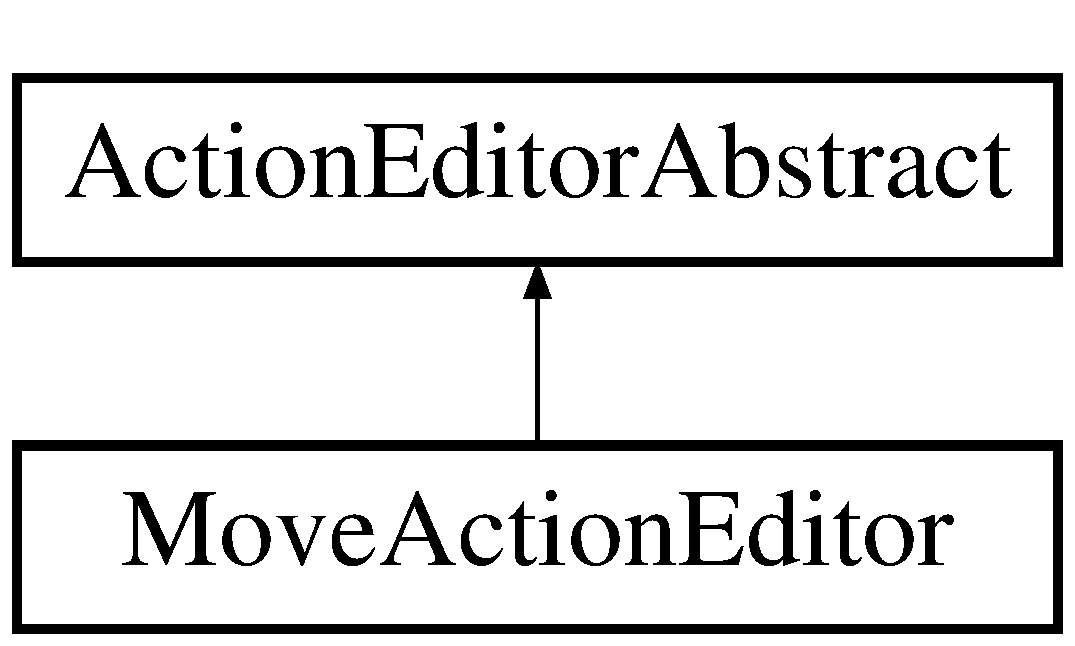
\includegraphics[height=2.000000cm]{class_move_action_editor}
\end{center}
\end{figure}
\subsection*{Public Member Functions}
\begin{DoxyCompactItemize}
\item 
\mbox{\hyperlink{class_move_action_editor_aa29a42691c56079aec9a9c22cbadb994}{Move\+Action\+Editor}} (\mbox{\hyperlink{class_move_action}{Move\+Action}} a)
\item 
void \mbox{\hyperlink{class_move_action_editor_a68dfb286dc1f7ea843b2916d12f0de26}{set\+Direction}} (\mbox{\hyperlink{_move_action_8cs_a9e4683fdca765fb08e2d0e5f7f57c162}{move\+Dir}} direction)
\end{DoxyCompactItemize}
\subsection*{Additional Inherited Members}


\subsection{Constructor \& Destructor Documentation}
\mbox{\Hypertarget{class_move_action_editor_aa29a42691c56079aec9a9c22cbadb994}\label{class_move_action_editor_aa29a42691c56079aec9a9c22cbadb994}} 
\index{Move\+Action\+Editor@{Move\+Action\+Editor}!Move\+Action\+Editor@{Move\+Action\+Editor}}
\index{Move\+Action\+Editor@{Move\+Action\+Editor}!Move\+Action\+Editor@{Move\+Action\+Editor}}
\subsubsection{\texorpdfstring{Move\+Action\+Editor()}{MoveActionEditor()}}
{\footnotesize\ttfamily Move\+Action\+Editor.\+Move\+Action\+Editor (\begin{DoxyParamCaption}\item[{\mbox{\hyperlink{class_move_action}{Move\+Action}}}]{a }\end{DoxyParamCaption})}



\subsection{Member Function Documentation}
\mbox{\Hypertarget{class_move_action_editor_a68dfb286dc1f7ea843b2916d12f0de26}\label{class_move_action_editor_a68dfb286dc1f7ea843b2916d12f0de26}} 
\index{Move\+Action\+Editor@{Move\+Action\+Editor}!set\+Direction@{set\+Direction}}
\index{set\+Direction@{set\+Direction}!Move\+Action\+Editor@{Move\+Action\+Editor}}
\subsubsection{\texorpdfstring{set\+Direction()}{setDirection()}}
{\footnotesize\ttfamily void Move\+Action\+Editor.\+set\+Direction (\begin{DoxyParamCaption}\item[{\mbox{\hyperlink{_move_action_8cs_a9e4683fdca765fb08e2d0e5f7f57c162}{move\+Dir}}}]{direction }\end{DoxyParamCaption})}



The documentation for this class was generated from the following file\+:\begin{DoxyCompactItemize}
\item 
\mbox{\hyperlink{_move_action_editor_8cs}{Move\+Action\+Editor.\+cs}}\end{DoxyCompactItemize}

\hypertarget{class_network}{}\section{Network Class Reference}
\label{class_network}\index{Network@{Network}}


A neural network of a creature, which consists of layers of nodes.  


Inheritance diagram for Network\+:\begin{figure}[H]
\begin{center}
\leavevmode
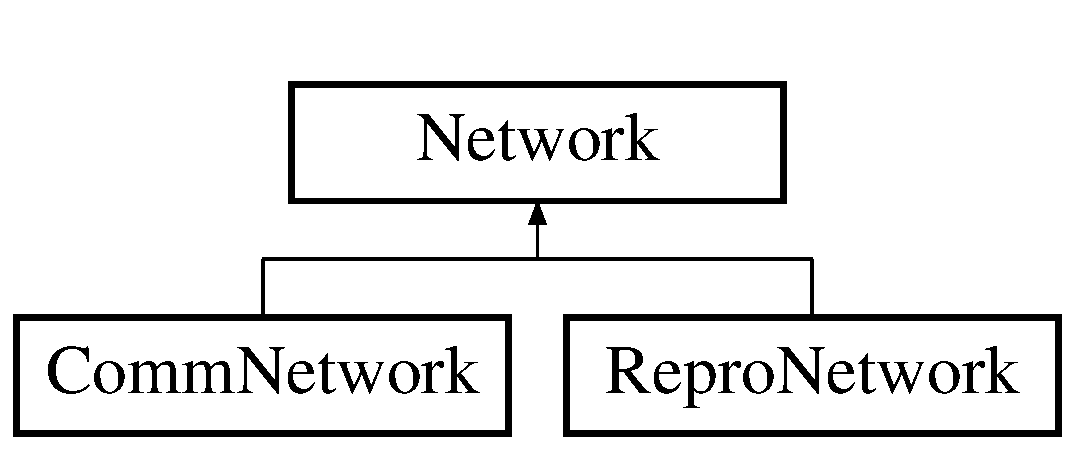
\includegraphics[height=2.000000cm]{class_network}
\end{center}
\end{figure}
\subsection*{Public Member Functions}
\begin{DoxyCompactItemize}
\item 
void \mbox{\hyperlink{class_network_a8285772739069a17a6cf3407208c25cb}{feed\+Forward}} ()
\begin{DoxyCompactList}\small\item\em Calls update value on each node in each layer \end{DoxyCompactList}\item 
\mbox{\hyperlink{class_network}{Network}} \mbox{\hyperlink{class_network_a08970b95e111e12a0463719c959db247}{get\+Shallow\+Copy}} ()
\end{DoxyCompactItemize}
\subsection*{Public Attributes}
\begin{DoxyCompactItemize}
\item 
List$<$ List$<$ \mbox{\hyperlink{class_node}{Node}} $>$ $>$ \mbox{\hyperlink{class_network_a5575fb3cc8b86da6ff8ffed15634e4b4}{net}} = new List$<$List$<$\mbox{\hyperlink{class_node}{Node}}$>$$>$()
\item 
string \mbox{\hyperlink{class_network_a9d47011c0cdd1c2c2a17f487fc20aa74}{name}}
\item 
int \mbox{\hyperlink{class_network_a28e1ac9d80508cd8bb52624e4e1efede}{in\+Layer}}
\end{DoxyCompactItemize}


\subsection{Detailed Description}
A neural network of a creature, which consists of layers of nodes. 



\subsection{Member Function Documentation}
\mbox{\Hypertarget{class_network_a8285772739069a17a6cf3407208c25cb}\label{class_network_a8285772739069a17a6cf3407208c25cb}} 
\index{Network@{Network}!feed\+Forward@{feed\+Forward}}
\index{feed\+Forward@{feed\+Forward}!Network@{Network}}
\subsubsection{\texorpdfstring{feed\+Forward()}{feedForward()}}
{\footnotesize\ttfamily void Network.\+feed\+Forward (\begin{DoxyParamCaption}{ }\end{DoxyParamCaption})}



Calls update value on each node in each layer 

\mbox{\Hypertarget{class_network_a08970b95e111e12a0463719c959db247}\label{class_network_a08970b95e111e12a0463719c959db247}} 
\index{Network@{Network}!get\+Shallow\+Copy@{get\+Shallow\+Copy}}
\index{get\+Shallow\+Copy@{get\+Shallow\+Copy}!Network@{Network}}
\subsubsection{\texorpdfstring{get\+Shallow\+Copy()}{getShallowCopy()}}
{\footnotesize\ttfamily \mbox{\hyperlink{class_network}{Network}} Network.\+get\+Shallow\+Copy (\begin{DoxyParamCaption}{ }\end{DoxyParamCaption})}



\subsection{Member Data Documentation}
\mbox{\Hypertarget{class_network_a28e1ac9d80508cd8bb52624e4e1efede}\label{class_network_a28e1ac9d80508cd8bb52624e4e1efede}} 
\index{Network@{Network}!in\+Layer@{in\+Layer}}
\index{in\+Layer@{in\+Layer}!Network@{Network}}
\subsubsection{\texorpdfstring{in\+Layer}{inLayer}}
{\footnotesize\ttfamily int Network.\+in\+Layer}

\mbox{\Hypertarget{class_network_a9d47011c0cdd1c2c2a17f487fc20aa74}\label{class_network_a9d47011c0cdd1c2c2a17f487fc20aa74}} 
\index{Network@{Network}!name@{name}}
\index{name@{name}!Network@{Network}}
\subsubsection{\texorpdfstring{name}{name}}
{\footnotesize\ttfamily string Network.\+name}

\mbox{\Hypertarget{class_network_a5575fb3cc8b86da6ff8ffed15634e4b4}\label{class_network_a5575fb3cc8b86da6ff8ffed15634e4b4}} 
\index{Network@{Network}!net@{net}}
\index{net@{net}!Network@{Network}}
\subsubsection{\texorpdfstring{net}{net}}
{\footnotesize\ttfamily List$<$List$<$\mbox{\hyperlink{class_node}{Node}}$>$ $>$ Network.\+net = new List$<$List$<$\mbox{\hyperlink{class_node}{Node}}$>$$>$()}



The documentation for this class was generated from the following file\+:\begin{DoxyCompactItemize}
\item 
\mbox{\hyperlink{_network_8cs}{Network.\+cs}}\end{DoxyCompactItemize}

\hypertarget{class_network_editor}{}\section{Network\+Editor Class Reference}
\label{class_network_editor}\index{Network\+Editor@{Network\+Editor}}


A\+PI for \mbox{\hyperlink{class_network}{Network}} objects. Stored by Ecosystem\+Creator.  


\subsection*{Public Member Functions}
\begin{DoxyCompactItemize}
\item 
\mbox{\hyperlink{class_network_editor_a8e9b3df4a6b328ee2d42318a82160faa}{Network\+Editor}} (\mbox{\hyperlink{class_network}{Network}} net, \mbox{\hyperlink{class_creature_editor}{Creature\+Editor}} \mbox{\hyperlink{class_network_editor_ac21fdc9f2b2211e5c79e05658d65b119}{parent\+Creature\+Creator}})
\item 
void \mbox{\hyperlink{class_network_editor_ac6cb833b0655afc32cb87323b96cd18d}{initialize\+Network}} ()
\item 
void \mbox{\hyperlink{class_network_editor_a9424b0712de79d74664e75822a39baf7}{set\+Name}} (string name)
\item 
void \mbox{\hyperlink{class_network_editor_aa0b9ca558f67b306d9ebacd6b797f723}{set\+In\+Layer}} (int layer)
\item 
void \mbox{\hyperlink{class_network_editor_aa81908526dda169d2b29161460f9b0e2}{save\+Node}} ()
\item 
\mbox{\hyperlink{class_node_editor}{Node\+Editor}} \mbox{\hyperlink{class_network_editor_a3958da3c1d8c016ba28e6ffc44a7e35f}{add\+Node}} (int layer)
\end{DoxyCompactItemize}
\subsection*{Public Attributes}
\begin{DoxyCompactItemize}
\item 
\mbox{\hyperlink{class_network}{Network}} \mbox{\hyperlink{class_network_editor_ad7a7f511e42a332743dc2abb223ca2c4}{network}}
\item 
\mbox{\hyperlink{class_node_editor}{Node\+Editor}} \mbox{\hyperlink{class_network_editor_a877324ecefb6e6371a0572fc4a57b116}{node\+Creator}}
\item 
\mbox{\hyperlink{class_creature_editor}{Creature\+Editor}} \mbox{\hyperlink{class_network_editor_ac21fdc9f2b2211e5c79e05658d65b119}{parent\+Creature\+Creator}}
\end{DoxyCompactItemize}


\subsection{Detailed Description}
A\+PI for \mbox{\hyperlink{class_network}{Network}} objects. Stored by Ecosystem\+Creator. 



\subsection{Constructor \& Destructor Documentation}
\mbox{\Hypertarget{class_network_editor_a8e9b3df4a6b328ee2d42318a82160faa}\label{class_network_editor_a8e9b3df4a6b328ee2d42318a82160faa}} 
\index{Network\+Editor@{Network\+Editor}!Network\+Editor@{Network\+Editor}}
\index{Network\+Editor@{Network\+Editor}!Network\+Editor@{Network\+Editor}}
\subsubsection{\texorpdfstring{Network\+Editor()}{NetworkEditor()}}
{\footnotesize\ttfamily Network\+Editor.\+Network\+Editor (\begin{DoxyParamCaption}\item[{\mbox{\hyperlink{class_network}{Network}}}]{net,  }\item[{\mbox{\hyperlink{class_creature_editor}{Creature\+Editor}}}]{parent\+Creature\+Creator }\end{DoxyParamCaption})}



\subsection{Member Function Documentation}
\mbox{\Hypertarget{class_network_editor_a3958da3c1d8c016ba28e6ffc44a7e35f}\label{class_network_editor_a3958da3c1d8c016ba28e6ffc44a7e35f}} 
\index{Network\+Editor@{Network\+Editor}!add\+Node@{add\+Node}}
\index{add\+Node@{add\+Node}!Network\+Editor@{Network\+Editor}}
\subsubsection{\texorpdfstring{add\+Node()}{addNode()}}
{\footnotesize\ttfamily \mbox{\hyperlink{class_node_editor}{Node\+Editor}} Network\+Editor.\+add\+Node (\begin{DoxyParamCaption}\item[{int}]{layer }\end{DoxyParamCaption})}

\mbox{\Hypertarget{class_network_editor_ac6cb833b0655afc32cb87323b96cd18d}\label{class_network_editor_ac6cb833b0655afc32cb87323b96cd18d}} 
\index{Network\+Editor@{Network\+Editor}!initialize\+Network@{initialize\+Network}}
\index{initialize\+Network@{initialize\+Network}!Network\+Editor@{Network\+Editor}}
\subsubsection{\texorpdfstring{initialize\+Network()}{initializeNetwork()}}
{\footnotesize\ttfamily void Network\+Editor.\+initialize\+Network (\begin{DoxyParamCaption}{ }\end{DoxyParamCaption})}

\mbox{\Hypertarget{class_network_editor_aa81908526dda169d2b29161460f9b0e2}\label{class_network_editor_aa81908526dda169d2b29161460f9b0e2}} 
\index{Network\+Editor@{Network\+Editor}!save\+Node@{save\+Node}}
\index{save\+Node@{save\+Node}!Network\+Editor@{Network\+Editor}}
\subsubsection{\texorpdfstring{save\+Node()}{saveNode()}}
{\footnotesize\ttfamily void Network\+Editor.\+save\+Node (\begin{DoxyParamCaption}{ }\end{DoxyParamCaption})}

\mbox{\Hypertarget{class_network_editor_aa0b9ca558f67b306d9ebacd6b797f723}\label{class_network_editor_aa0b9ca558f67b306d9ebacd6b797f723}} 
\index{Network\+Editor@{Network\+Editor}!set\+In\+Layer@{set\+In\+Layer}}
\index{set\+In\+Layer@{set\+In\+Layer}!Network\+Editor@{Network\+Editor}}
\subsubsection{\texorpdfstring{set\+In\+Layer()}{setInLayer()}}
{\footnotesize\ttfamily void Network\+Editor.\+set\+In\+Layer (\begin{DoxyParamCaption}\item[{int}]{layer }\end{DoxyParamCaption})}

\mbox{\Hypertarget{class_network_editor_a9424b0712de79d74664e75822a39baf7}\label{class_network_editor_a9424b0712de79d74664e75822a39baf7}} 
\index{Network\+Editor@{Network\+Editor}!set\+Name@{set\+Name}}
\index{set\+Name@{set\+Name}!Network\+Editor@{Network\+Editor}}
\subsubsection{\texorpdfstring{set\+Name()}{setName()}}
{\footnotesize\ttfamily void Network\+Editor.\+set\+Name (\begin{DoxyParamCaption}\item[{string}]{name }\end{DoxyParamCaption})}



\subsection{Member Data Documentation}
\mbox{\Hypertarget{class_network_editor_ad7a7f511e42a332743dc2abb223ca2c4}\label{class_network_editor_ad7a7f511e42a332743dc2abb223ca2c4}} 
\index{Network\+Editor@{Network\+Editor}!network@{network}}
\index{network@{network}!Network\+Editor@{Network\+Editor}}
\subsubsection{\texorpdfstring{network}{network}}
{\footnotesize\ttfamily \mbox{\hyperlink{class_network}{Network}} Network\+Editor.\+network}

\mbox{\Hypertarget{class_network_editor_a877324ecefb6e6371a0572fc4a57b116}\label{class_network_editor_a877324ecefb6e6371a0572fc4a57b116}} 
\index{Network\+Editor@{Network\+Editor}!node\+Creator@{node\+Creator}}
\index{node\+Creator@{node\+Creator}!Network\+Editor@{Network\+Editor}}
\subsubsection{\texorpdfstring{node\+Creator}{nodeCreator}}
{\footnotesize\ttfamily \mbox{\hyperlink{class_node_editor}{Node\+Editor}} Network\+Editor.\+node\+Creator}

\mbox{\Hypertarget{class_network_editor_ac21fdc9f2b2211e5c79e05658d65b119}\label{class_network_editor_ac21fdc9f2b2211e5c79e05658d65b119}} 
\index{Network\+Editor@{Network\+Editor}!parent\+Creature\+Creator@{parent\+Creature\+Creator}}
\index{parent\+Creature\+Creator@{parent\+Creature\+Creator}!Network\+Editor@{Network\+Editor}}
\subsubsection{\texorpdfstring{parent\+Creature\+Creator}{parentCreatureCreator}}
{\footnotesize\ttfamily \mbox{\hyperlink{class_creature_editor}{Creature\+Editor}} Network\+Editor.\+parent\+Creature\+Creator}



The documentation for this class was generated from the following file\+:\begin{DoxyCompactItemize}
\item 
\mbox{\hyperlink{_network_editor_8cs}{Network\+Editor.\+cs}}\end{DoxyCompactItemize}

\hypertarget{class_node}{}\section{Node Class Reference}
\label{class_node}\index{Node@{Node}}
\subsection*{Public Member Functions}
\begin{DoxyCompactItemize}
\item 
void \mbox{\hyperlink{class_node_a6700b2928da6ac5fcac8431d6f16597e}{append\+Input\+Node}} (\mbox{\hyperlink{class_node}{Node}} new\+Node)
\begin{DoxyCompactList}\small\item\em Adds a node to the array of input nodes. \end{DoxyCompactList}\item 
bool \mbox{\hyperlink{class_node_ae35ca95be4806e6a3f81617d888f724f}{remove\+Node}} (int remove\+Index)
\begin{DoxyCompactList}\small\item\em Remove node from input nodes. \end{DoxyCompactList}\end{DoxyCompactItemize}
\subsection*{Properties}
\begin{DoxyCompactItemize}
\item 
float \mbox{\hyperlink{class_node_a4d82b89fd1d72cc0184763279a3811dc}{value}}\hspace{0.3cm}{\ttfamily  \mbox{[}get, set\mbox{]}}
\begin{DoxyCompactList}\small\item\em The value of the node takes on based on it\textquotesingle{}s inputs and activation function. \end{DoxyCompactList}\end{DoxyCompactItemize}


\subsection{Member Function Documentation}
\mbox{\Hypertarget{class_node_a6700b2928da6ac5fcac8431d6f16597e}\label{class_node_a6700b2928da6ac5fcac8431d6f16597e}} 
\index{Node@{Node}!append\+Input\+Node@{append\+Input\+Node}}
\index{append\+Input\+Node@{append\+Input\+Node}!Node@{Node}}
\subsubsection{\texorpdfstring{append\+Input\+Node()}{appendInputNode()}}
{\footnotesize\ttfamily void Node.\+append\+Input\+Node (\begin{DoxyParamCaption}\item[{\mbox{\hyperlink{class_node}{Node}}}]{new\+Node }\end{DoxyParamCaption})}



Adds a node to the array of input nodes. 

\mbox{\Hypertarget{class_node_ae35ca95be4806e6a3f81617d888f724f}\label{class_node_ae35ca95be4806e6a3f81617d888f724f}} 
\index{Node@{Node}!remove\+Node@{remove\+Node}}
\index{remove\+Node@{remove\+Node}!Node@{Node}}
\subsubsection{\texorpdfstring{remove\+Node()}{removeNode()}}
{\footnotesize\ttfamily bool Node.\+remove\+Node (\begin{DoxyParamCaption}\item[{int}]{remove\+Index }\end{DoxyParamCaption})}



Remove node from input nodes. 


\begin{DoxyParams}{Parameters}
{\em remove\+Index} & Index of node to remove.\\
\hline
\end{DoxyParams}


\subsection{Property Documentation}
\mbox{\Hypertarget{class_node_a4d82b89fd1d72cc0184763279a3811dc}\label{class_node_a4d82b89fd1d72cc0184763279a3811dc}} 
\index{Node@{Node}!value@{value}}
\index{value@{value}!Node@{Node}}
\subsubsection{\texorpdfstring{value}{value}}
{\footnotesize\ttfamily float Node.\+value\hspace{0.3cm}{\ttfamily [get]}, {\ttfamily [set]}}



The value of the node takes on based on it\textquotesingle{}s inputs and activation function. 



The documentation for this class was generated from the following file\+:\begin{DoxyCompactItemize}
\item 
C\+:/\+Users/\+Brett/\+Documents/\+Git\+Hub/\+Unity/\+Eco\+Net/\+Assets/\+Scripts/Node.\+cs\end{DoxyCompactItemize}

\hypertarget{class_node_editor}{}\section{Node\+Editor Class Reference}
\label{class_node_editor}\index{Node\+Editor@{Node\+Editor}}


A\+PI for storing different kinds of specific node creators. ex. -\/ could wrap a Sensory\+Input\+Node\+Creator. Stored by Network\+Creator.  


\subsection*{Public Member Functions}
\begin{DoxyCompactItemize}
\item 
\mbox{\hyperlink{class_node_editor_abd0642bacf3934685527b94425770f64}{Node\+Editor}} (int \+\_\+layer, \mbox{\hyperlink{class_network_editor}{Network\+Editor}} parent\+Net\+Creator)
\item 
void \mbox{\hyperlink{class_node_editor_a24174978502582ab68d487d35f38d029}{set\+Creator}} (\mbox{\hyperlink{_node_editor_8cs_afc5d9fc086bcd57827af91c5d369b625}{Node\+Creator\+Type}} type)
\item 
\mbox{\hyperlink{interface_node_editor_interface}{Node\+Editor\+Interface}} \mbox{\hyperlink{class_node_editor_acdd21c090158fa8bbfd636bec7d86309}{get\+Node\+Creator}} ()
\item 
\mbox{\hyperlink{class_node}{Node}} \mbox{\hyperlink{class_node_editor_a42b9d431ac444320d4d628d13868c19f}{get\+Created\+Node}} ()
\end{DoxyCompactItemize}
\subsection*{Public Attributes}
\begin{DoxyCompactItemize}
\item 
int \mbox{\hyperlink{class_node_editor_aebb0d7bfb182de466d69abe21ab21fbb}{node\+Layer}}
\end{DoxyCompactItemize}


\subsection{Detailed Description}
A\+PI for storing different kinds of specific node creators. ex. -\/ could wrap a Sensory\+Input\+Node\+Creator. Stored by Network\+Creator. 



\subsection{Constructor \& Destructor Documentation}
\mbox{\Hypertarget{class_node_editor_abd0642bacf3934685527b94425770f64}\label{class_node_editor_abd0642bacf3934685527b94425770f64}} 
\index{Node\+Editor@{Node\+Editor}!Node\+Editor@{Node\+Editor}}
\index{Node\+Editor@{Node\+Editor}!Node\+Editor@{Node\+Editor}}
\subsubsection{\texorpdfstring{Node\+Editor()}{NodeEditor()}}
{\footnotesize\ttfamily Node\+Editor.\+Node\+Editor (\begin{DoxyParamCaption}\item[{int}]{\+\_\+layer,  }\item[{\mbox{\hyperlink{class_network_editor}{Network\+Editor}}}]{parent\+Net\+Creator }\end{DoxyParamCaption})}



\subsection{Member Function Documentation}
\mbox{\Hypertarget{class_node_editor_a42b9d431ac444320d4d628d13868c19f}\label{class_node_editor_a42b9d431ac444320d4d628d13868c19f}} 
\index{Node\+Editor@{Node\+Editor}!get\+Created\+Node@{get\+Created\+Node}}
\index{get\+Created\+Node@{get\+Created\+Node}!Node\+Editor@{Node\+Editor}}
\subsubsection{\texorpdfstring{get\+Created\+Node()}{getCreatedNode()}}
{\footnotesize\ttfamily \mbox{\hyperlink{class_node}{Node}} Node\+Editor.\+get\+Created\+Node (\begin{DoxyParamCaption}{ }\end{DoxyParamCaption})}

\mbox{\Hypertarget{class_node_editor_acdd21c090158fa8bbfd636bec7d86309}\label{class_node_editor_acdd21c090158fa8bbfd636bec7d86309}} 
\index{Node\+Editor@{Node\+Editor}!get\+Node\+Creator@{get\+Node\+Creator}}
\index{get\+Node\+Creator@{get\+Node\+Creator}!Node\+Editor@{Node\+Editor}}
\subsubsection{\texorpdfstring{get\+Node\+Creator()}{getNodeCreator()}}
{\footnotesize\ttfamily \mbox{\hyperlink{interface_node_editor_interface}{Node\+Editor\+Interface}} Node\+Editor.\+get\+Node\+Creator (\begin{DoxyParamCaption}{ }\end{DoxyParamCaption})}

\mbox{\Hypertarget{class_node_editor_a24174978502582ab68d487d35f38d029}\label{class_node_editor_a24174978502582ab68d487d35f38d029}} 
\index{Node\+Editor@{Node\+Editor}!set\+Creator@{set\+Creator}}
\index{set\+Creator@{set\+Creator}!Node\+Editor@{Node\+Editor}}
\subsubsection{\texorpdfstring{set\+Creator()}{setCreator()}}
{\footnotesize\ttfamily void Node\+Editor.\+set\+Creator (\begin{DoxyParamCaption}\item[{\mbox{\hyperlink{_node_editor_8cs_afc5d9fc086bcd57827af91c5d369b625}{Node\+Creator\+Type}}}]{type }\end{DoxyParamCaption})}



\subsection{Member Data Documentation}
\mbox{\Hypertarget{class_node_editor_aebb0d7bfb182de466d69abe21ab21fbb}\label{class_node_editor_aebb0d7bfb182de466d69abe21ab21fbb}} 
\index{Node\+Editor@{Node\+Editor}!node\+Layer@{node\+Layer}}
\index{node\+Layer@{node\+Layer}!Node\+Editor@{Node\+Editor}}
\subsubsection{\texorpdfstring{node\+Layer}{nodeLayer}}
{\footnotesize\ttfamily int Node\+Editor.\+node\+Layer}



The documentation for this class was generated from the following file\+:\begin{DoxyCompactItemize}
\item 
\mbox{\hyperlink{_node_editor_8cs}{Node\+Editor.\+cs}}\end{DoxyCompactItemize}

\hypertarget{interface_node_editor_interface}{}\section{Node\+Editor\+Interface Interface Reference}
\label{interface_node_editor_interface}\index{Node\+Editor\+Interface@{Node\+Editor\+Interface}}


Interface that allows all specific node creator objects to be stored by Node\+Creator class.  


Inheritance diagram for Node\+Editor\+Interface\+:\begin{figure}[H]
\begin{center}
\leavevmode
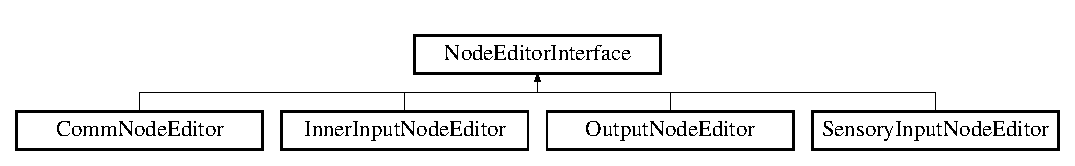
\includegraphics[height=1.783440cm]{interface_node_editor_interface}
\end{center}
\end{figure}
\subsection*{Public Member Functions}
\begin{DoxyCompactItemize}
\item 
\mbox{\hyperlink{class_node}{Node}} \mbox{\hyperlink{interface_node_editor_interface_a56e2abaedf17d7fbf2be90d521ec9363}{get\+Node}} ()
\end{DoxyCompactItemize}


\subsection{Detailed Description}
Interface that allows all specific node creator objects to be stored by Node\+Creator class. 



\subsection{Member Function Documentation}
\mbox{\Hypertarget{interface_node_editor_interface_a56e2abaedf17d7fbf2be90d521ec9363}\label{interface_node_editor_interface_a56e2abaedf17d7fbf2be90d521ec9363}} 
\index{Node\+Editor\+Interface@{Node\+Editor\+Interface}!get\+Node@{get\+Node}}
\index{get\+Node@{get\+Node}!Node\+Editor\+Interface@{Node\+Editor\+Interface}}
\subsubsection{\texorpdfstring{get\+Node()}{getNode()}}
{\footnotesize\ttfamily \mbox{\hyperlink{class_node}{Node}} Node\+Editor\+Interface.\+get\+Node (\begin{DoxyParamCaption}{ }\end{DoxyParamCaption})}



Implemented in \mbox{\hyperlink{class_comm_node_editor_ad578649fe7c3775e0b91c1acdb5e738a}{Comm\+Node\+Editor}}, \mbox{\hyperlink{class_sensory_input_node_editor_ab6f6a94004254d8bba213a6e91fcc946}{Sensory\+Input\+Node\+Editor}}, \mbox{\hyperlink{class_inner_input_node_editor_a211d3bfaad897b853671c9c61366779f}{Inner\+Input\+Node\+Editor}}, and \mbox{\hyperlink{class_output_node_editor_afca854ca2a34703a1becfee48da12631}{Output\+Node\+Editor}}.



The documentation for this interface was generated from the following file\+:\begin{DoxyCompactItemize}
\item 
\mbox{\hyperlink{_node_editor_interface_8cs}{Node\+Editor\+Interface.\+cs}}\end{DoxyCompactItemize}

\hypertarget{class_non_input_node}{}\section{Non\+Input\+Node Class Reference}
\label{class_non_input_node}\index{Non\+Input\+Node@{Non\+Input\+Node}}


Encompasses hidden nodes (which use this class directly) and output nodes (which use the \mbox{\hyperlink{class_output_node}{Output\+Node}} class).  


Inheritance diagram for Non\+Input\+Node\+:\begin{figure}[H]
\begin{center}
\leavevmode
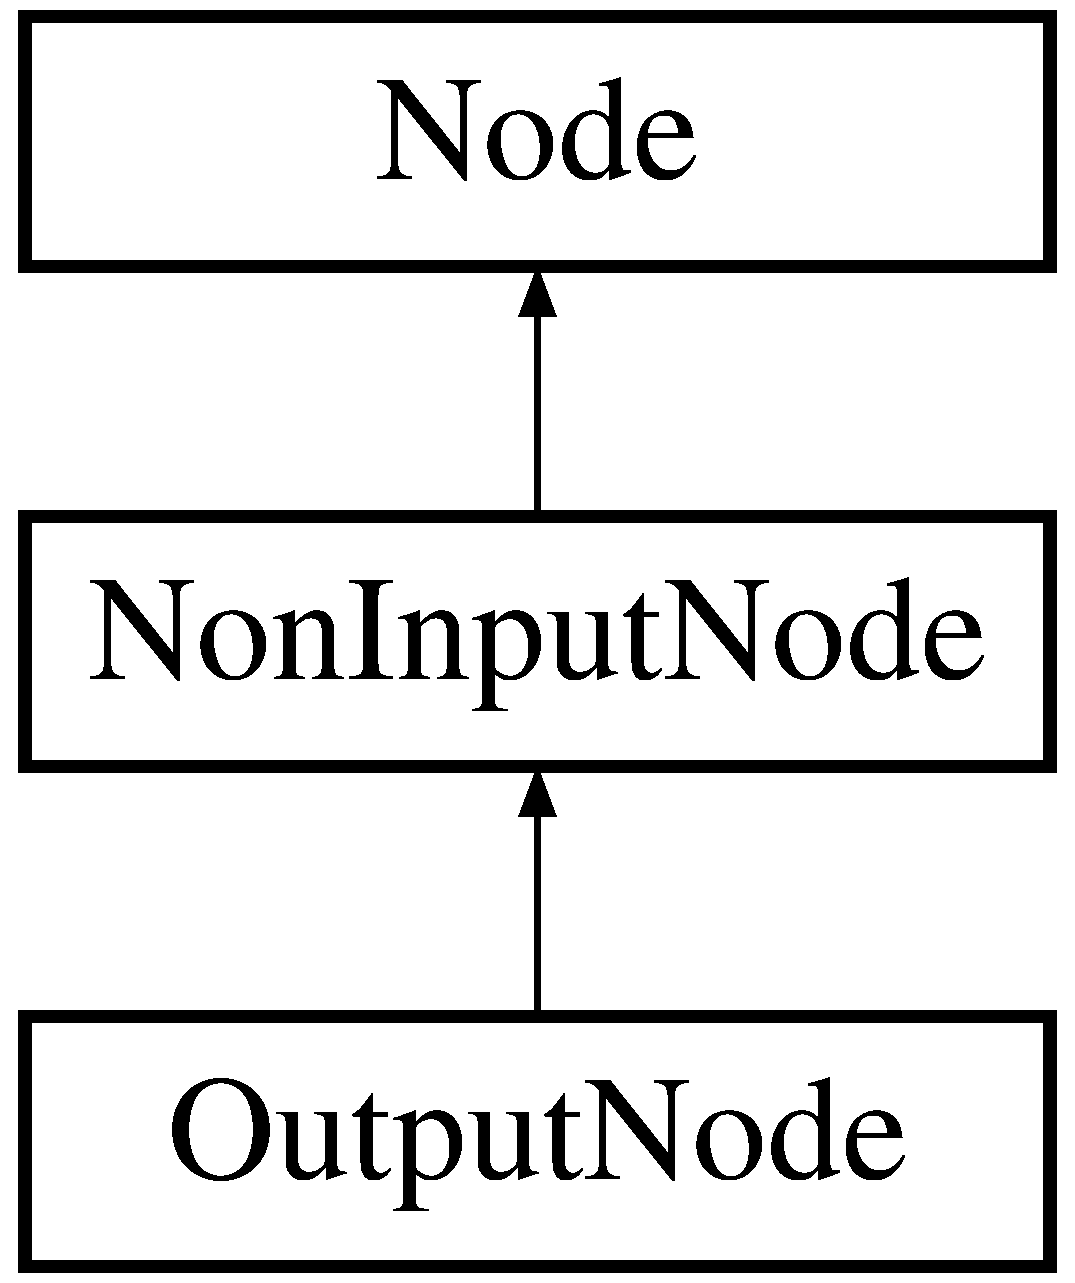
\includegraphics[height=3.000000cm]{class_non_input_node}
\end{center}
\end{figure}
\subsection*{Public Member Functions}
\begin{DoxyCompactItemize}
\item 
\mbox{\hyperlink{class_non_input_node_a3facbd688b6a772cf1259420238255c8}{Non\+Input\+Node}} ()
\item 
\mbox{\hyperlink{class_non_input_node_a2805394951d04ebab266877c5723132b}{Non\+Input\+Node}} (\mbox{\hyperlink{class_network}{Network}} \mbox{\hyperlink{class_non_input_node_ac79615aee9a2b85aa9c31f98451da37a}{parent\+Net}}, int \mbox{\hyperlink{class_non_input_node_a5614e202d11fbe3ca55ec88e6e803cb8}{layer}})
\item 
override void \mbox{\hyperlink{class_non_input_node_a075d0278c5500f0d2455a3d8eeb04f55}{update\+Value}} ()
\begin{DoxyCompactList}\small\item\em Updates node value \end{DoxyCompactList}\item 
void \mbox{\hyperlink{class_non_input_node_a458bad6de5c7d5e82d85998d456be3ec}{append\+Prev\+Node}} (\mbox{\hyperlink{class_node}{Node}} new\+Node)
\item 
void \mbox{\hyperlink{class_non_input_node_a2318ad48afb979bc655d67b4f7f6dca2}{remove\+Prev\+Node}} (int index)
\item 
void \mbox{\hyperlink{class_non_input_node_a7c1d1f3d6b86394ade501797f1733472}{set\+Prev\+Node\+Weight}} (int index, float weight)
\item 
float \mbox{\hyperlink{class_non_input_node_ab6f9a79605853e0e4aec8c7034345aa0}{perform\+Activ\+Behavior}} (float input)
\begin{DoxyCompactList}\small\item\em Calls activation function of activ\+Behavior. \end{DoxyCompactList}\item 
void \mbox{\hyperlink{class_non_input_node_a44be3d4caebaa9f9fc8d6c9659bdb674}{set\+Activ\+Behavior}} (\mbox{\hyperlink{interface_activation_behavior}{Activation\+Behavior}} behavior)
\begin{DoxyCompactList}\small\item\em Sets a new activation behavior, thus altering the activation function. \end{DoxyCompactList}\item 
void \mbox{\hyperlink{class_non_input_node_a703986aac246746c6269522d7a03e13e}{reset\+All\+Previous\+Nodes}} ()
\begin{DoxyCompactList}\small\item\em Sets prev\+Nodes to include all nodes in previous layer. Resets nodes and weights \end{DoxyCompactList}\item 
void \mbox{\hyperlink{class_non_input_node_abd2e854cfd7c52bc91bd8a14df972a79}{assign\+Prev\+Nodes}} ()
\item 
float \mbox{\hyperlink{class_non_input_node_a8368526477286eba442737fa000fef16}{generate\+New\+Random\+Weight}} ()
\item 
void \mbox{\hyperlink{class_non_input_node_a7d9c289b2c8d666a3d9ae69e1f536cfa}{reset\+Rand}} ()
\item 
object \mbox{\hyperlink{class_non_input_node_a4aadcefa9b95598c8d8c985e0e690041}{clone}} ()
\item 
void \mbox{\hyperlink{class_non_input_node_a67de84779fee28a0db7b5b10b84f9db6}{print\+Inputs\+And\+Weights}} ()
\end{DoxyCompactItemize}
\subsection*{Public Attributes}
\begin{DoxyCompactItemize}
\item 
List$<$ int $>$ \mbox{\hyperlink{class_non_input_node_a8bbea5d8230dac63fd88d987e5eb41a7}{taboo\+Prev\+Node\+Indicies}} = new List$<$int$>$()
\item 
List$<$ \mbox{\hyperlink{class_node}{Node}} $>$ \mbox{\hyperlink{class_non_input_node_ad4f05e0609cd43ea03edfd9937f4e3b9}{prev\+Nodes}} = new List$<$\mbox{\hyperlink{class_node}{Node}}$>$()
\item 
List$<$ float $>$ \mbox{\hyperlink{class_non_input_node_a4c2ddced3cd3b741bbf5253dd69661d2}{weights}} = new List$<$float$>$()
\begin{DoxyCompactList}\small\item\em List of weights to be multiplied by previous node values. \end{DoxyCompactList}\item 
\mbox{\hyperlink{class_network}{Network}} \mbox{\hyperlink{class_non_input_node_ac79615aee9a2b85aa9c31f98451da37a}{parent\+Net}}
\item 
int \mbox{\hyperlink{class_non_input_node_a5614e202d11fbe3ca55ec88e6e803cb8}{layer}}
\end{DoxyCompactItemize}
\subsection*{Protected Attributes}
\begin{DoxyCompactItemize}
\item 
\mbox{\hyperlink{interface_activation_behavior}{Activation\+Behavior}} \mbox{\hyperlink{class_non_input_node_ab33f9a611488e5dfcb697941736f5cfc}{activ\+Behavior}}
\begin{DoxyCompactList}\small\item\em Holds an object that carries out an activation function. \end{DoxyCompactList}\end{DoxyCompactItemize}


\subsection{Detailed Description}
Encompasses hidden nodes (which use this class directly) and output nodes (which use the \mbox{\hyperlink{class_output_node}{Output\+Node}} class). 



\subsection{Constructor \& Destructor Documentation}
\mbox{\Hypertarget{class_non_input_node_a3facbd688b6a772cf1259420238255c8}\label{class_non_input_node_a3facbd688b6a772cf1259420238255c8}} 
\index{Non\+Input\+Node@{Non\+Input\+Node}!Non\+Input\+Node@{Non\+Input\+Node}}
\index{Non\+Input\+Node@{Non\+Input\+Node}!Non\+Input\+Node@{Non\+Input\+Node}}
\subsubsection{\texorpdfstring{Non\+Input\+Node()}{NonInputNode()}\hspace{0.1cm}{\footnotesize\ttfamily [1/2]}}
{\footnotesize\ttfamily Non\+Input\+Node.\+Non\+Input\+Node (\begin{DoxyParamCaption}{ }\end{DoxyParamCaption})}

\mbox{\Hypertarget{class_non_input_node_a2805394951d04ebab266877c5723132b}\label{class_non_input_node_a2805394951d04ebab266877c5723132b}} 
\index{Non\+Input\+Node@{Non\+Input\+Node}!Non\+Input\+Node@{Non\+Input\+Node}}
\index{Non\+Input\+Node@{Non\+Input\+Node}!Non\+Input\+Node@{Non\+Input\+Node}}
\subsubsection{\texorpdfstring{Non\+Input\+Node()}{NonInputNode()}\hspace{0.1cm}{\footnotesize\ttfamily [2/2]}}
{\footnotesize\ttfamily Non\+Input\+Node.\+Non\+Input\+Node (\begin{DoxyParamCaption}\item[{\mbox{\hyperlink{class_network}{Network}}}]{parent\+Net,  }\item[{int}]{layer }\end{DoxyParamCaption})}



\subsection{Member Function Documentation}
\mbox{\Hypertarget{class_non_input_node_a458bad6de5c7d5e82d85998d456be3ec}\label{class_non_input_node_a458bad6de5c7d5e82d85998d456be3ec}} 
\index{Non\+Input\+Node@{Non\+Input\+Node}!append\+Prev\+Node@{append\+Prev\+Node}}
\index{append\+Prev\+Node@{append\+Prev\+Node}!Non\+Input\+Node@{Non\+Input\+Node}}
\subsubsection{\texorpdfstring{append\+Prev\+Node()}{appendPrevNode()}}
{\footnotesize\ttfamily void Non\+Input\+Node.\+append\+Prev\+Node (\begin{DoxyParamCaption}\item[{\mbox{\hyperlink{class_node}{Node}}}]{new\+Node }\end{DoxyParamCaption})}

\mbox{\Hypertarget{class_non_input_node_abd2e854cfd7c52bc91bd8a14df972a79}\label{class_non_input_node_abd2e854cfd7c52bc91bd8a14df972a79}} 
\index{Non\+Input\+Node@{Non\+Input\+Node}!assign\+Prev\+Nodes@{assign\+Prev\+Nodes}}
\index{assign\+Prev\+Nodes@{assign\+Prev\+Nodes}!Non\+Input\+Node@{Non\+Input\+Node}}
\subsubsection{\texorpdfstring{assign\+Prev\+Nodes()}{assignPrevNodes()}}
{\footnotesize\ttfamily void Non\+Input\+Node.\+assign\+Prev\+Nodes (\begin{DoxyParamCaption}{ }\end{DoxyParamCaption})}

\mbox{\Hypertarget{class_non_input_node_a4aadcefa9b95598c8d8c985e0e690041}\label{class_non_input_node_a4aadcefa9b95598c8d8c985e0e690041}} 
\index{Non\+Input\+Node@{Non\+Input\+Node}!clone@{clone}}
\index{clone@{clone}!Non\+Input\+Node@{Non\+Input\+Node}}
\subsubsection{\texorpdfstring{clone()}{clone()}}
{\footnotesize\ttfamily object Non\+Input\+Node.\+clone (\begin{DoxyParamCaption}{ }\end{DoxyParamCaption})}

\mbox{\Hypertarget{class_non_input_node_a8368526477286eba442737fa000fef16}\label{class_non_input_node_a8368526477286eba442737fa000fef16}} 
\index{Non\+Input\+Node@{Non\+Input\+Node}!generate\+New\+Random\+Weight@{generate\+New\+Random\+Weight}}
\index{generate\+New\+Random\+Weight@{generate\+New\+Random\+Weight}!Non\+Input\+Node@{Non\+Input\+Node}}
\subsubsection{\texorpdfstring{generate\+New\+Random\+Weight()}{generateNewRandomWeight()}}
{\footnotesize\ttfamily float Non\+Input\+Node.\+generate\+New\+Random\+Weight (\begin{DoxyParamCaption}{ }\end{DoxyParamCaption})}

\mbox{\Hypertarget{class_non_input_node_ab6f9a79605853e0e4aec8c7034345aa0}\label{class_non_input_node_ab6f9a79605853e0e4aec8c7034345aa0}} 
\index{Non\+Input\+Node@{Non\+Input\+Node}!perform\+Activ\+Behavior@{perform\+Activ\+Behavior}}
\index{perform\+Activ\+Behavior@{perform\+Activ\+Behavior}!Non\+Input\+Node@{Non\+Input\+Node}}
\subsubsection{\texorpdfstring{perform\+Activ\+Behavior()}{performActivBehavior()}}
{\footnotesize\ttfamily float Non\+Input\+Node.\+perform\+Activ\+Behavior (\begin{DoxyParamCaption}\item[{float}]{input }\end{DoxyParamCaption})}



Calls activation function of activ\+Behavior. 

\mbox{\Hypertarget{class_non_input_node_a67de84779fee28a0db7b5b10b84f9db6}\label{class_non_input_node_a67de84779fee28a0db7b5b10b84f9db6}} 
\index{Non\+Input\+Node@{Non\+Input\+Node}!print\+Inputs\+And\+Weights@{print\+Inputs\+And\+Weights}}
\index{print\+Inputs\+And\+Weights@{print\+Inputs\+And\+Weights}!Non\+Input\+Node@{Non\+Input\+Node}}
\subsubsection{\texorpdfstring{print\+Inputs\+And\+Weights()}{printInputsAndWeights()}}
{\footnotesize\ttfamily void Non\+Input\+Node.\+print\+Inputs\+And\+Weights (\begin{DoxyParamCaption}{ }\end{DoxyParamCaption})}

\mbox{\Hypertarget{class_non_input_node_a2318ad48afb979bc655d67b4f7f6dca2}\label{class_non_input_node_a2318ad48afb979bc655d67b4f7f6dca2}} 
\index{Non\+Input\+Node@{Non\+Input\+Node}!remove\+Prev\+Node@{remove\+Prev\+Node}}
\index{remove\+Prev\+Node@{remove\+Prev\+Node}!Non\+Input\+Node@{Non\+Input\+Node}}
\subsubsection{\texorpdfstring{remove\+Prev\+Node()}{removePrevNode()}}
{\footnotesize\ttfamily void Non\+Input\+Node.\+remove\+Prev\+Node (\begin{DoxyParamCaption}\item[{int}]{index }\end{DoxyParamCaption})}

\mbox{\Hypertarget{class_non_input_node_a703986aac246746c6269522d7a03e13e}\label{class_non_input_node_a703986aac246746c6269522d7a03e13e}} 
\index{Non\+Input\+Node@{Non\+Input\+Node}!reset\+All\+Previous\+Nodes@{reset\+All\+Previous\+Nodes}}
\index{reset\+All\+Previous\+Nodes@{reset\+All\+Previous\+Nodes}!Non\+Input\+Node@{Non\+Input\+Node}}
\subsubsection{\texorpdfstring{reset\+All\+Previous\+Nodes()}{resetAllPreviousNodes()}}
{\footnotesize\ttfamily void Non\+Input\+Node.\+reset\+All\+Previous\+Nodes (\begin{DoxyParamCaption}{ }\end{DoxyParamCaption})}



Sets prev\+Nodes to include all nodes in previous layer. Resets nodes and weights 

\mbox{\Hypertarget{class_non_input_node_a7d9c289b2c8d666a3d9ae69e1f536cfa}\label{class_non_input_node_a7d9c289b2c8d666a3d9ae69e1f536cfa}} 
\index{Non\+Input\+Node@{Non\+Input\+Node}!reset\+Rand@{reset\+Rand}}
\index{reset\+Rand@{reset\+Rand}!Non\+Input\+Node@{Non\+Input\+Node}}
\subsubsection{\texorpdfstring{reset\+Rand()}{resetRand()}}
{\footnotesize\ttfamily void Non\+Input\+Node.\+reset\+Rand (\begin{DoxyParamCaption}{ }\end{DoxyParamCaption})}

\mbox{\Hypertarget{class_non_input_node_a44be3d4caebaa9f9fc8d6c9659bdb674}\label{class_non_input_node_a44be3d4caebaa9f9fc8d6c9659bdb674}} 
\index{Non\+Input\+Node@{Non\+Input\+Node}!set\+Activ\+Behavior@{set\+Activ\+Behavior}}
\index{set\+Activ\+Behavior@{set\+Activ\+Behavior}!Non\+Input\+Node@{Non\+Input\+Node}}
\subsubsection{\texorpdfstring{set\+Activ\+Behavior()}{setActivBehavior()}}
{\footnotesize\ttfamily void Non\+Input\+Node.\+set\+Activ\+Behavior (\begin{DoxyParamCaption}\item[{\mbox{\hyperlink{interface_activation_behavior}{Activation\+Behavior}}}]{behavior }\end{DoxyParamCaption})}



Sets a new activation behavior, thus altering the activation function. 

\mbox{\Hypertarget{class_non_input_node_a7c1d1f3d6b86394ade501797f1733472}\label{class_non_input_node_a7c1d1f3d6b86394ade501797f1733472}} 
\index{Non\+Input\+Node@{Non\+Input\+Node}!set\+Prev\+Node\+Weight@{set\+Prev\+Node\+Weight}}
\index{set\+Prev\+Node\+Weight@{set\+Prev\+Node\+Weight}!Non\+Input\+Node@{Non\+Input\+Node}}
\subsubsection{\texorpdfstring{set\+Prev\+Node\+Weight()}{setPrevNodeWeight()}}
{\footnotesize\ttfamily void Non\+Input\+Node.\+set\+Prev\+Node\+Weight (\begin{DoxyParamCaption}\item[{int}]{index,  }\item[{float}]{weight }\end{DoxyParamCaption})}


\begin{DoxyParams}{Parameters}
{\em index} & Index of previous node.\\
\hline
{\em value} & Weight coming from previous node.\\
\hline
\end{DoxyParams}
\mbox{\Hypertarget{class_non_input_node_a075d0278c5500f0d2455a3d8eeb04f55}\label{class_non_input_node_a075d0278c5500f0d2455a3d8eeb04f55}} 
\index{Non\+Input\+Node@{Non\+Input\+Node}!update\+Value@{update\+Value}}
\index{update\+Value@{update\+Value}!Non\+Input\+Node@{Non\+Input\+Node}}
\subsubsection{\texorpdfstring{update\+Value()}{updateValue()}}
{\footnotesize\ttfamily override void Non\+Input\+Node.\+update\+Value (\begin{DoxyParamCaption}{ }\end{DoxyParamCaption})\hspace{0.3cm}{\ttfamily [virtual]}}



Updates node value 



Implements \mbox{\hyperlink{class_node_a85ebd0e36c25430570b94f923afd2a62}{Node}}.



\subsection{Member Data Documentation}
\mbox{\Hypertarget{class_non_input_node_ab33f9a611488e5dfcb697941736f5cfc}\label{class_non_input_node_ab33f9a611488e5dfcb697941736f5cfc}} 
\index{Non\+Input\+Node@{Non\+Input\+Node}!activ\+Behavior@{activ\+Behavior}}
\index{activ\+Behavior@{activ\+Behavior}!Non\+Input\+Node@{Non\+Input\+Node}}
\subsubsection{\texorpdfstring{activ\+Behavior}{activBehavior}}
{\footnotesize\ttfamily \mbox{\hyperlink{interface_activation_behavior}{Activation\+Behavior}} Non\+Input\+Node.\+activ\+Behavior\hspace{0.3cm}{\ttfamily [protected]}}



Holds an object that carries out an activation function. 

\mbox{\Hypertarget{class_non_input_node_a5614e202d11fbe3ca55ec88e6e803cb8}\label{class_non_input_node_a5614e202d11fbe3ca55ec88e6e803cb8}} 
\index{Non\+Input\+Node@{Non\+Input\+Node}!layer@{layer}}
\index{layer@{layer}!Non\+Input\+Node@{Non\+Input\+Node}}
\subsubsection{\texorpdfstring{layer}{layer}}
{\footnotesize\ttfamily int Non\+Input\+Node.\+layer}

\mbox{\Hypertarget{class_non_input_node_ac79615aee9a2b85aa9c31f98451da37a}\label{class_non_input_node_ac79615aee9a2b85aa9c31f98451da37a}} 
\index{Non\+Input\+Node@{Non\+Input\+Node}!parent\+Net@{parent\+Net}}
\index{parent\+Net@{parent\+Net}!Non\+Input\+Node@{Non\+Input\+Node}}
\subsubsection{\texorpdfstring{parent\+Net}{parentNet}}
{\footnotesize\ttfamily \mbox{\hyperlink{class_network}{Network}} Non\+Input\+Node.\+parent\+Net}

\mbox{\Hypertarget{class_non_input_node_ad4f05e0609cd43ea03edfd9937f4e3b9}\label{class_non_input_node_ad4f05e0609cd43ea03edfd9937f4e3b9}} 
\index{Non\+Input\+Node@{Non\+Input\+Node}!prev\+Nodes@{prev\+Nodes}}
\index{prev\+Nodes@{prev\+Nodes}!Non\+Input\+Node@{Non\+Input\+Node}}
\subsubsection{\texorpdfstring{prev\+Nodes}{prevNodes}}
{\footnotesize\ttfamily List$<$\mbox{\hyperlink{class_node}{Node}}$>$ Non\+Input\+Node.\+prev\+Nodes = new List$<$\mbox{\hyperlink{class_node}{Node}}$>$()}

\mbox{\Hypertarget{class_non_input_node_a8bbea5d8230dac63fd88d987e5eb41a7}\label{class_non_input_node_a8bbea5d8230dac63fd88d987e5eb41a7}} 
\index{Non\+Input\+Node@{Non\+Input\+Node}!taboo\+Prev\+Node\+Indicies@{taboo\+Prev\+Node\+Indicies}}
\index{taboo\+Prev\+Node\+Indicies@{taboo\+Prev\+Node\+Indicies}!Non\+Input\+Node@{Non\+Input\+Node}}
\subsubsection{\texorpdfstring{taboo\+Prev\+Node\+Indicies}{tabooPrevNodeIndicies}}
{\footnotesize\ttfamily List$<$int$>$ Non\+Input\+Node.\+taboo\+Prev\+Node\+Indicies = new List$<$int$>$()}

\mbox{\Hypertarget{class_non_input_node_a4c2ddced3cd3b741bbf5253dd69661d2}\label{class_non_input_node_a4c2ddced3cd3b741bbf5253dd69661d2}} 
\index{Non\+Input\+Node@{Non\+Input\+Node}!weights@{weights}}
\index{weights@{weights}!Non\+Input\+Node@{Non\+Input\+Node}}
\subsubsection{\texorpdfstring{weights}{weights}}
{\footnotesize\ttfamily List$<$float$>$ Non\+Input\+Node.\+weights = new List$<$float$>$()}



List of weights to be multiplied by previous node values. 



The documentation for this class was generated from the following file\+:\begin{DoxyCompactItemize}
\item 
\mbox{\hyperlink{_non_input_node_8cs}{Non\+Input\+Node.\+cs}}\end{DoxyCompactItemize}

\hypertarget{class_output_node}{}\section{Output\+Node Class Reference}
\label{class_output_node}\index{Output\+Node@{Output\+Node}}


Maps a the value of the node (as calculated by \mbox{\hyperlink{class_non_input_node}{Non\+Input\+Node}} methods) to an action.  


Inheritance diagram for Output\+Node\+:\begin{figure}[H]
\begin{center}
\leavevmode
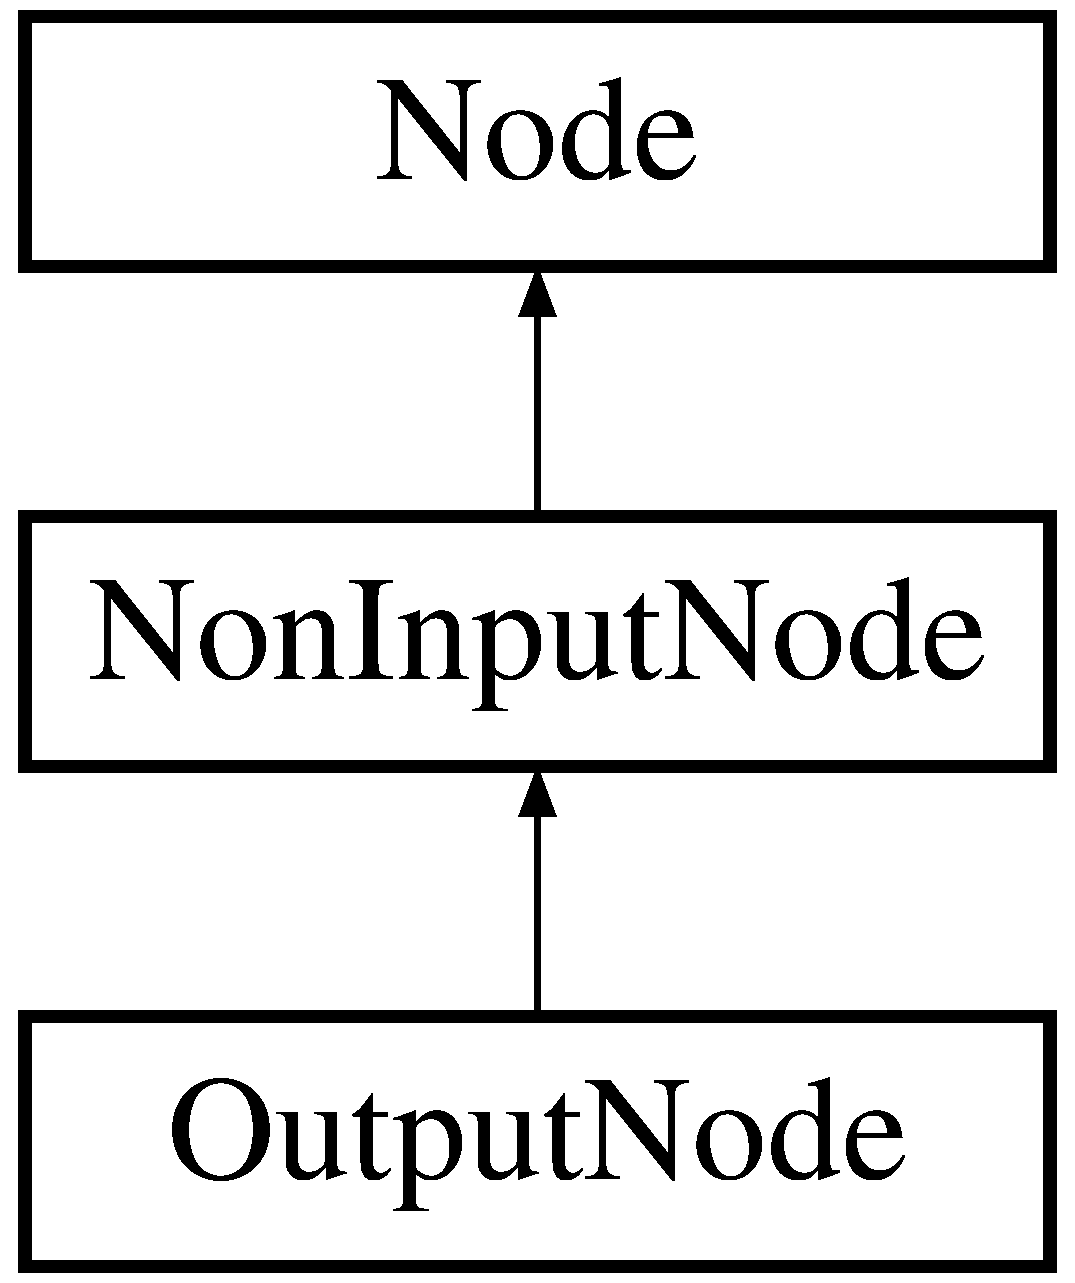
\includegraphics[height=3.000000cm]{class_output_node}
\end{center}
\end{figure}
\subsection*{Public Member Functions}
\begin{DoxyCompactItemize}
\item 
\mbox{\hyperlink{class_output_node_abf3c6c3ab42fb35f64e894a15f0d057e}{Output\+Node}} ()
\item 
\mbox{\hyperlink{class_output_node_ab065c6d98c883b8416acbc5add709013}{Output\+Node}} (\mbox{\hyperlink{class_creature}{Creature}} \mbox{\hyperlink{class_output_node_a4be36782d750ac8d91c0f51628d353fb}{parent\+Creature}}, \mbox{\hyperlink{class_network}{Network}} \mbox{\hyperlink{class_non_input_node_ac79615aee9a2b85aa9c31f98451da37a}{parent\+Net}}, int \mbox{\hyperlink{class_non_input_node_a5614e202d11fbe3ca55ec88e6e803cb8}{layer}})
\item 
void \mbox{\hyperlink{class_output_node_a6d6a43ded165156d825fd039487f2a10}{add\+Action\+If\+Active}} ()
\begin{DoxyCompactList}\small\item\em Adds its action to the action queue based on probability returned from the activation function. \end{DoxyCompactList}\item 
void \mbox{\hyperlink{class_output_node_aeb94c02a334d514de5a0bcb474778f41}{set\+Action}} (string \mbox{\hyperlink{class_output_node_a48299e62ef82f692d8656d0efec1b236}{action\+Key}})
\item 
\mbox{\hyperlink{class_output_node}{Output\+Node}} \mbox{\hyperlink{class_output_node_af4524058cc5cbb2fbd29aac4b970395f}{clone}} ()
\end{DoxyCompactItemize}
\subsection*{Public Attributes}
\begin{DoxyCompactItemize}
\item 
\mbox{\hyperlink{class_action}{Action}} \mbox{\hyperlink{class_output_node_a330eb0533baf20b237f93627106d6b56}{action}}
\item 
\mbox{\hyperlink{class_creature}{Creature}} \mbox{\hyperlink{class_output_node_a4be36782d750ac8d91c0f51628d353fb}{parent\+Creature}}
\item 
string \mbox{\hyperlink{class_output_node_a48299e62ef82f692d8656d0efec1b236}{action\+Key}}
\end{DoxyCompactItemize}
\subsection*{Additional Inherited Members}


\subsection{Detailed Description}
Maps a the value of the node (as calculated by \mbox{\hyperlink{class_non_input_node}{Non\+Input\+Node}} methods) to an action. 



\subsection{Constructor \& Destructor Documentation}
\mbox{\Hypertarget{class_output_node_abf3c6c3ab42fb35f64e894a15f0d057e}\label{class_output_node_abf3c6c3ab42fb35f64e894a15f0d057e}} 
\index{Output\+Node@{Output\+Node}!Output\+Node@{Output\+Node}}
\index{Output\+Node@{Output\+Node}!Output\+Node@{Output\+Node}}
\subsubsection{\texorpdfstring{Output\+Node()}{OutputNode()}\hspace{0.1cm}{\footnotesize\ttfamily [1/2]}}
{\footnotesize\ttfamily Output\+Node.\+Output\+Node (\begin{DoxyParamCaption}{ }\end{DoxyParamCaption})}

\mbox{\Hypertarget{class_output_node_ab065c6d98c883b8416acbc5add709013}\label{class_output_node_ab065c6d98c883b8416acbc5add709013}} 
\index{Output\+Node@{Output\+Node}!Output\+Node@{Output\+Node}}
\index{Output\+Node@{Output\+Node}!Output\+Node@{Output\+Node}}
\subsubsection{\texorpdfstring{Output\+Node()}{OutputNode()}\hspace{0.1cm}{\footnotesize\ttfamily [2/2]}}
{\footnotesize\ttfamily Output\+Node.\+Output\+Node (\begin{DoxyParamCaption}\item[{\mbox{\hyperlink{class_creature}{Creature}}}]{parent\+Creature,  }\item[{\mbox{\hyperlink{class_network}{Network}}}]{parent\+Net,  }\item[{int}]{layer }\end{DoxyParamCaption})}



\subsection{Member Function Documentation}
\mbox{\Hypertarget{class_output_node_a6d6a43ded165156d825fd039487f2a10}\label{class_output_node_a6d6a43ded165156d825fd039487f2a10}} 
\index{Output\+Node@{Output\+Node}!add\+Action\+If\+Active@{add\+Action\+If\+Active}}
\index{add\+Action\+If\+Active@{add\+Action\+If\+Active}!Output\+Node@{Output\+Node}}
\subsubsection{\texorpdfstring{add\+Action\+If\+Active()}{addActionIfActive()}}
{\footnotesize\ttfamily void Output\+Node.\+add\+Action\+If\+Active (\begin{DoxyParamCaption}{ }\end{DoxyParamCaption})}



Adds its action to the action queue based on probability returned from the activation function. 

\mbox{\Hypertarget{class_output_node_af4524058cc5cbb2fbd29aac4b970395f}\label{class_output_node_af4524058cc5cbb2fbd29aac4b970395f}} 
\index{Output\+Node@{Output\+Node}!clone@{clone}}
\index{clone@{clone}!Output\+Node@{Output\+Node}}
\subsubsection{\texorpdfstring{clone()}{clone()}}
{\footnotesize\ttfamily \mbox{\hyperlink{class_output_node}{Output\+Node}} Output\+Node.\+clone (\begin{DoxyParamCaption}{ }\end{DoxyParamCaption})}

\mbox{\Hypertarget{class_output_node_aeb94c02a334d514de5a0bcb474778f41}\label{class_output_node_aeb94c02a334d514de5a0bcb474778f41}} 
\index{Output\+Node@{Output\+Node}!set\+Action@{set\+Action}}
\index{set\+Action@{set\+Action}!Output\+Node@{Output\+Node}}
\subsubsection{\texorpdfstring{set\+Action()}{setAction()}}
{\footnotesize\ttfamily void Output\+Node.\+set\+Action (\begin{DoxyParamCaption}\item[{string}]{action\+Key }\end{DoxyParamCaption})}



\subsection{Member Data Documentation}
\mbox{\Hypertarget{class_output_node_a330eb0533baf20b237f93627106d6b56}\label{class_output_node_a330eb0533baf20b237f93627106d6b56}} 
\index{Output\+Node@{Output\+Node}!action@{action}}
\index{action@{action}!Output\+Node@{Output\+Node}}
\subsubsection{\texorpdfstring{action}{action}}
{\footnotesize\ttfamily \mbox{\hyperlink{class_action}{Action}} Output\+Node.\+action}

\mbox{\Hypertarget{class_output_node_a48299e62ef82f692d8656d0efec1b236}\label{class_output_node_a48299e62ef82f692d8656d0efec1b236}} 
\index{Output\+Node@{Output\+Node}!action\+Key@{action\+Key}}
\index{action\+Key@{action\+Key}!Output\+Node@{Output\+Node}}
\subsubsection{\texorpdfstring{action\+Key}{actionKey}}
{\footnotesize\ttfamily string Output\+Node.\+action\+Key}

\mbox{\Hypertarget{class_output_node_a4be36782d750ac8d91c0f51628d353fb}\label{class_output_node_a4be36782d750ac8d91c0f51628d353fb}} 
\index{Output\+Node@{Output\+Node}!parent\+Creature@{parent\+Creature}}
\index{parent\+Creature@{parent\+Creature}!Output\+Node@{Output\+Node}}
\subsubsection{\texorpdfstring{parent\+Creature}{parentCreature}}
{\footnotesize\ttfamily \mbox{\hyperlink{class_creature}{Creature}} Output\+Node.\+parent\+Creature}



The documentation for this class was generated from the following file\+:\begin{DoxyCompactItemize}
\item 
\mbox{\hyperlink{_output_node_8cs}{Output\+Node.\+cs}}\end{DoxyCompactItemize}

\hypertarget{class_output_node_editor}{}\section{Output\+Node\+Editor Class Reference}
\label{class_output_node_editor}\index{Output\+Node\+Editor@{Output\+Node\+Editor}}


A\+PI for Output\+Nodes.  


Inheritance diagram for Output\+Node\+Editor\+:\begin{figure}[H]
\begin{center}
\leavevmode
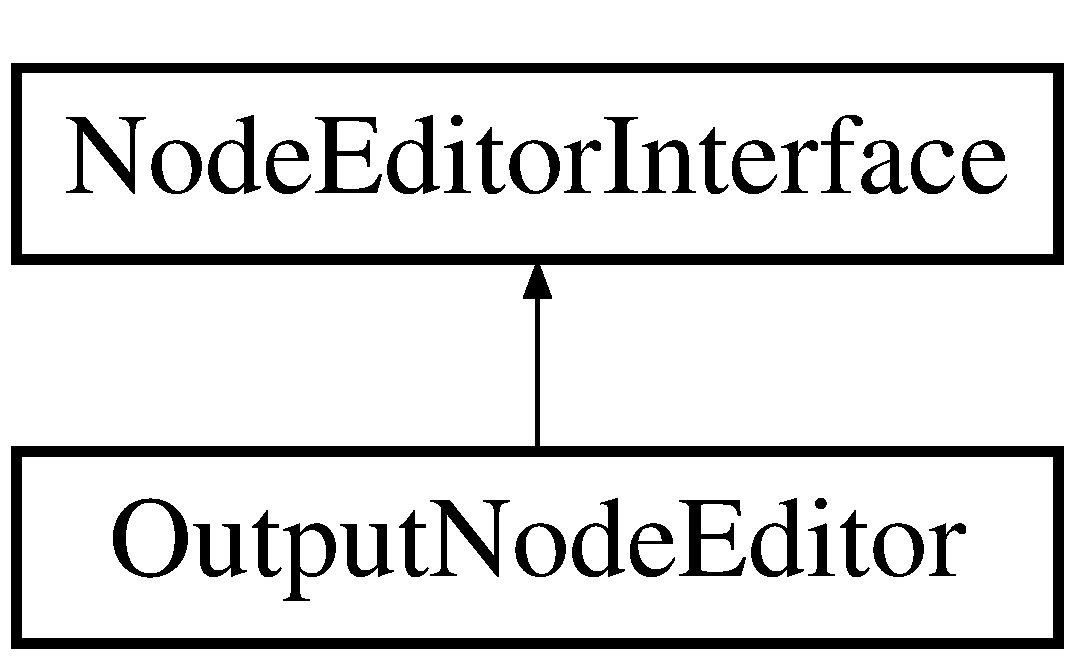
\includegraphics[height=2.000000cm]{class_output_node_editor}
\end{center}
\end{figure}
\subsection*{Public Member Functions}
\begin{DoxyCompactItemize}
\item 
\mbox{\hyperlink{class_output_node_editor_a623838b68ab06f8409a371e119bf70ac}{Output\+Node\+Editor}} (\mbox{\hyperlink{class_output_node}{Output\+Node}} \mbox{\hyperlink{class_output_node_editor_a78bb1baa0dddf7eb38ac12357ddea2f6}{fo\+Node}}, int \mbox{\hyperlink{class_output_node_editor_acbb36568e920b010b900395a59959e9d}{node\+Layer}})
\item 
\mbox{\hyperlink{class_node}{Node}} \mbox{\hyperlink{class_output_node_editor_afca854ca2a34703a1becfee48da12631}{get\+Node}} ()
\item 
void \mbox{\hyperlink{class_output_node_editor_a04ec0f0500518d70391de298bcb07513}{set\+Action}} (string action\+Key)
\item 
void \mbox{\hyperlink{class_output_node_editor_a832616727e8d1ab1a1a5e8c8d793ac0d}{set\+Activation\+Function}} (\mbox{\hyperlink{_non_input_node_8cs_a832a6943e91e304dea9608c4ae2818e7}{Activation\+Behavior\+Types}} activ\+Type)
\end{DoxyCompactItemize}
\subsection*{Public Attributes}
\begin{DoxyCompactItemize}
\item 
\mbox{\hyperlink{class_output_node}{Output\+Node}} \mbox{\hyperlink{class_output_node_editor_a78bb1baa0dddf7eb38ac12357ddea2f6}{fo\+Node}}
\item 
int \mbox{\hyperlink{class_output_node_editor_acbb36568e920b010b900395a59959e9d}{node\+Layer}}
\end{DoxyCompactItemize}


\subsection{Detailed Description}
A\+PI for Output\+Nodes. 



\subsection{Constructor \& Destructor Documentation}
\mbox{\Hypertarget{class_output_node_editor_a623838b68ab06f8409a371e119bf70ac}\label{class_output_node_editor_a623838b68ab06f8409a371e119bf70ac}} 
\index{Output\+Node\+Editor@{Output\+Node\+Editor}!Output\+Node\+Editor@{Output\+Node\+Editor}}
\index{Output\+Node\+Editor@{Output\+Node\+Editor}!Output\+Node\+Editor@{Output\+Node\+Editor}}
\subsubsection{\texorpdfstring{Output\+Node\+Editor()}{OutputNodeEditor()}}
{\footnotesize\ttfamily Output\+Node\+Editor.\+Output\+Node\+Editor (\begin{DoxyParamCaption}\item[{\mbox{\hyperlink{class_output_node}{Output\+Node}}}]{fo\+Node,  }\item[{int}]{node\+Layer }\end{DoxyParamCaption})}



\subsection{Member Function Documentation}
\mbox{\Hypertarget{class_output_node_editor_afca854ca2a34703a1becfee48da12631}\label{class_output_node_editor_afca854ca2a34703a1becfee48da12631}} 
\index{Output\+Node\+Editor@{Output\+Node\+Editor}!get\+Node@{get\+Node}}
\index{get\+Node@{get\+Node}!Output\+Node\+Editor@{Output\+Node\+Editor}}
\subsubsection{\texorpdfstring{get\+Node()}{getNode()}}
{\footnotesize\ttfamily \mbox{\hyperlink{class_node}{Node}} Output\+Node\+Editor.\+get\+Node (\begin{DoxyParamCaption}{ }\end{DoxyParamCaption})}



Implements \mbox{\hyperlink{interface_node_editor_interface_a56e2abaedf17d7fbf2be90d521ec9363}{Node\+Editor\+Interface}}.

\mbox{\Hypertarget{class_output_node_editor_a04ec0f0500518d70391de298bcb07513}\label{class_output_node_editor_a04ec0f0500518d70391de298bcb07513}} 
\index{Output\+Node\+Editor@{Output\+Node\+Editor}!set\+Action@{set\+Action}}
\index{set\+Action@{set\+Action}!Output\+Node\+Editor@{Output\+Node\+Editor}}
\subsubsection{\texorpdfstring{set\+Action()}{setAction()}}
{\footnotesize\ttfamily void Output\+Node\+Editor.\+set\+Action (\begin{DoxyParamCaption}\item[{string}]{action\+Key }\end{DoxyParamCaption})}

\mbox{\Hypertarget{class_output_node_editor_a832616727e8d1ab1a1a5e8c8d793ac0d}\label{class_output_node_editor_a832616727e8d1ab1a1a5e8c8d793ac0d}} 
\index{Output\+Node\+Editor@{Output\+Node\+Editor}!set\+Activation\+Function@{set\+Activation\+Function}}
\index{set\+Activation\+Function@{set\+Activation\+Function}!Output\+Node\+Editor@{Output\+Node\+Editor}}
\subsubsection{\texorpdfstring{set\+Activation\+Function()}{setActivationFunction()}}
{\footnotesize\ttfamily void Output\+Node\+Editor.\+set\+Activation\+Function (\begin{DoxyParamCaption}\item[{\mbox{\hyperlink{_non_input_node_8cs_a832a6943e91e304dea9608c4ae2818e7}{Activation\+Behavior\+Types}}}]{activ\+Type }\end{DoxyParamCaption})}



\subsection{Member Data Documentation}
\mbox{\Hypertarget{class_output_node_editor_a78bb1baa0dddf7eb38ac12357ddea2f6}\label{class_output_node_editor_a78bb1baa0dddf7eb38ac12357ddea2f6}} 
\index{Output\+Node\+Editor@{Output\+Node\+Editor}!fo\+Node@{fo\+Node}}
\index{fo\+Node@{fo\+Node}!Output\+Node\+Editor@{Output\+Node\+Editor}}
\subsubsection{\texorpdfstring{fo\+Node}{foNode}}
{\footnotesize\ttfamily \mbox{\hyperlink{class_output_node}{Output\+Node}} Output\+Node\+Editor.\+fo\+Node}

\mbox{\Hypertarget{class_output_node_editor_acbb36568e920b010b900395a59959e9d}\label{class_output_node_editor_acbb36568e920b010b900395a59959e9d}} 
\index{Output\+Node\+Editor@{Output\+Node\+Editor}!node\+Layer@{node\+Layer}}
\index{node\+Layer@{node\+Layer}!Output\+Node\+Editor@{Output\+Node\+Editor}}
\subsubsection{\texorpdfstring{node\+Layer}{nodeLayer}}
{\footnotesize\ttfamily int Output\+Node\+Editor.\+node\+Layer}



The documentation for this class was generated from the following file\+:\begin{DoxyCompactItemize}
\item 
\mbox{\hyperlink{_output_node_editor_8cs}{Output\+Node\+Editor.\+cs}}\end{DoxyCompactItemize}

\hypertarget{class_population}{}\section{Population Class Reference}
\label{class_population}\index{Population@{Population}}


A population stores information about a list of creatures, including it\textquotesingle{}s founder, and initial variation.  


\subsection*{Public Member Functions}
\begin{DoxyCompactItemize}
\item 
\mbox{\hyperlink{class_creature}{Creature}} \mbox{\hyperlink{class_population_a72997a708270ddf7ae76faff9a97190e}{generate\+Member}} ()
\item 
\mbox{\hyperlink{class_population}{Population}} \mbox{\hyperlink{class_population_a910060609bb65d002204b871df9a6876}{shallow\+Copy}} ()
\end{DoxyCompactItemize}
\subsection*{Public Attributes}
\begin{DoxyCompactItemize}
\item 
List$<$ \mbox{\hyperlink{class_creature}{Creature}} $>$ \mbox{\hyperlink{class_population_a417192b3b7e2f3cd9e9d528752e6c340}{creatures}}
\item 
List$<$ \mbox{\hyperlink{class_creature}{Creature}} $>$ \mbox{\hyperlink{class_population_a69c9eb7cfdb0e5d269ae9ac24290762d}{offspring}} = new List$<$\mbox{\hyperlink{class_creature}{Creature}}$>$()
\item 
\mbox{\hyperlink{class_creature}{Creature}} \mbox{\hyperlink{class_population_ad823b4be605e706379c58ed2880ca7f4}{founder}}
\item 
float \mbox{\hyperlink{class_population_a6b94d7c76b73372f59e95368b301c8f0}{weight\+Standard\+Dev}}
\item 
float \mbox{\hyperlink{class_population_a84fda8156e0f5cf7a90178f879d070b0}{ability\+Standard\+Dev}}
\item 
float \mbox{\hyperlink{class_population_add38fbdaebb253fd3cc2375e36e4d2dc}{mutation\+Standard\+Dev}}
\item 
int \mbox{\hyperlink{class_population_a1df2f4121cc9396d17e0bbc6b8a14b81}{size}} = 0
\item 
int \mbox{\hyperlink{class_population_a8b2bc8fa877db5c7280bbc97b414acf3}{max\+Size}} = 1000
\end{DoxyCompactItemize}


\subsection{Detailed Description}
A population stores information about a list of creatures, including it\textquotesingle{}s founder, and initial variation. 



\subsection{Member Function Documentation}
\mbox{\Hypertarget{class_population_a72997a708270ddf7ae76faff9a97190e}\label{class_population_a72997a708270ddf7ae76faff9a97190e}} 
\index{Population@{Population}!generate\+Member@{generate\+Member}}
\index{generate\+Member@{generate\+Member}!Population@{Population}}
\subsubsection{\texorpdfstring{generate\+Member()}{generateMember()}}
{\footnotesize\ttfamily \mbox{\hyperlink{class_creature}{Creature}} Population.\+generate\+Member (\begin{DoxyParamCaption}{ }\end{DoxyParamCaption})}

\mbox{\Hypertarget{class_population_a910060609bb65d002204b871df9a6876}\label{class_population_a910060609bb65d002204b871df9a6876}} 
\index{Population@{Population}!shallow\+Copy@{shallow\+Copy}}
\index{shallow\+Copy@{shallow\+Copy}!Population@{Population}}
\subsubsection{\texorpdfstring{shallow\+Copy()}{shallowCopy()}}
{\footnotesize\ttfamily \mbox{\hyperlink{class_population}{Population}} Population.\+shallow\+Copy (\begin{DoxyParamCaption}{ }\end{DoxyParamCaption})}



\subsection{Member Data Documentation}
\mbox{\Hypertarget{class_population_a84fda8156e0f5cf7a90178f879d070b0}\label{class_population_a84fda8156e0f5cf7a90178f879d070b0}} 
\index{Population@{Population}!ability\+Standard\+Dev@{ability\+Standard\+Dev}}
\index{ability\+Standard\+Dev@{ability\+Standard\+Dev}!Population@{Population}}
\subsubsection{\texorpdfstring{ability\+Standard\+Dev}{abilityStandardDev}}
{\footnotesize\ttfamily float Population.\+ability\+Standard\+Dev}

\mbox{\Hypertarget{class_population_a417192b3b7e2f3cd9e9d528752e6c340}\label{class_population_a417192b3b7e2f3cd9e9d528752e6c340}} 
\index{Population@{Population}!creatures@{creatures}}
\index{creatures@{creatures}!Population@{Population}}
\subsubsection{\texorpdfstring{creatures}{creatures}}
{\footnotesize\ttfamily List$<$\mbox{\hyperlink{class_creature}{Creature}}$>$ Population.\+creatures}

\mbox{\Hypertarget{class_population_ad823b4be605e706379c58ed2880ca7f4}\label{class_population_ad823b4be605e706379c58ed2880ca7f4}} 
\index{Population@{Population}!founder@{founder}}
\index{founder@{founder}!Population@{Population}}
\subsubsection{\texorpdfstring{founder}{founder}}
{\footnotesize\ttfamily \mbox{\hyperlink{class_creature}{Creature}} Population.\+founder}

\mbox{\Hypertarget{class_population_a8b2bc8fa877db5c7280bbc97b414acf3}\label{class_population_a8b2bc8fa877db5c7280bbc97b414acf3}} 
\index{Population@{Population}!max\+Size@{max\+Size}}
\index{max\+Size@{max\+Size}!Population@{Population}}
\subsubsection{\texorpdfstring{max\+Size}{maxSize}}
{\footnotesize\ttfamily int Population.\+max\+Size = 1000}

\mbox{\Hypertarget{class_population_add38fbdaebb253fd3cc2375e36e4d2dc}\label{class_population_add38fbdaebb253fd3cc2375e36e4d2dc}} 
\index{Population@{Population}!mutation\+Standard\+Dev@{mutation\+Standard\+Dev}}
\index{mutation\+Standard\+Dev@{mutation\+Standard\+Dev}!Population@{Population}}
\subsubsection{\texorpdfstring{mutation\+Standard\+Dev}{mutationStandardDev}}
{\footnotesize\ttfamily float Population.\+mutation\+Standard\+Dev}

\mbox{\Hypertarget{class_population_a69c9eb7cfdb0e5d269ae9ac24290762d}\label{class_population_a69c9eb7cfdb0e5d269ae9ac24290762d}} 
\index{Population@{Population}!offspring@{offspring}}
\index{offspring@{offspring}!Population@{Population}}
\subsubsection{\texorpdfstring{offspring}{offspring}}
{\footnotesize\ttfamily List$<$\mbox{\hyperlink{class_creature}{Creature}}$>$ Population.\+offspring = new List$<$\mbox{\hyperlink{class_creature}{Creature}}$>$()}

\mbox{\Hypertarget{class_population_a1df2f4121cc9396d17e0bbc6b8a14b81}\label{class_population_a1df2f4121cc9396d17e0bbc6b8a14b81}} 
\index{Population@{Population}!size@{size}}
\index{size@{size}!Population@{Population}}
\subsubsection{\texorpdfstring{size}{size}}
{\footnotesize\ttfamily int Population.\+size = 0}

\mbox{\Hypertarget{class_population_a6b94d7c76b73372f59e95368b301c8f0}\label{class_population_a6b94d7c76b73372f59e95368b301c8f0}} 
\index{Population@{Population}!weight\+Standard\+Dev@{weight\+Standard\+Dev}}
\index{weight\+Standard\+Dev@{weight\+Standard\+Dev}!Population@{Population}}
\subsubsection{\texorpdfstring{weight\+Standard\+Dev}{weightStandardDev}}
{\footnotesize\ttfamily float Population.\+weight\+Standard\+Dev}



The documentation for this class was generated from the following file\+:\begin{DoxyCompactItemize}
\item 
\mbox{\hyperlink{_population_8cs}{Population.\+cs}}\end{DoxyCompactItemize}

\hypertarget{class_repro_action}{}\section{Repro\+Action Class Reference}
\label{class_repro_action}\index{Repro\+Action@{Repro\+Action}}
Inheritance diagram for Repro\+Action\+:\begin{figure}[H]
\begin{center}
\leavevmode
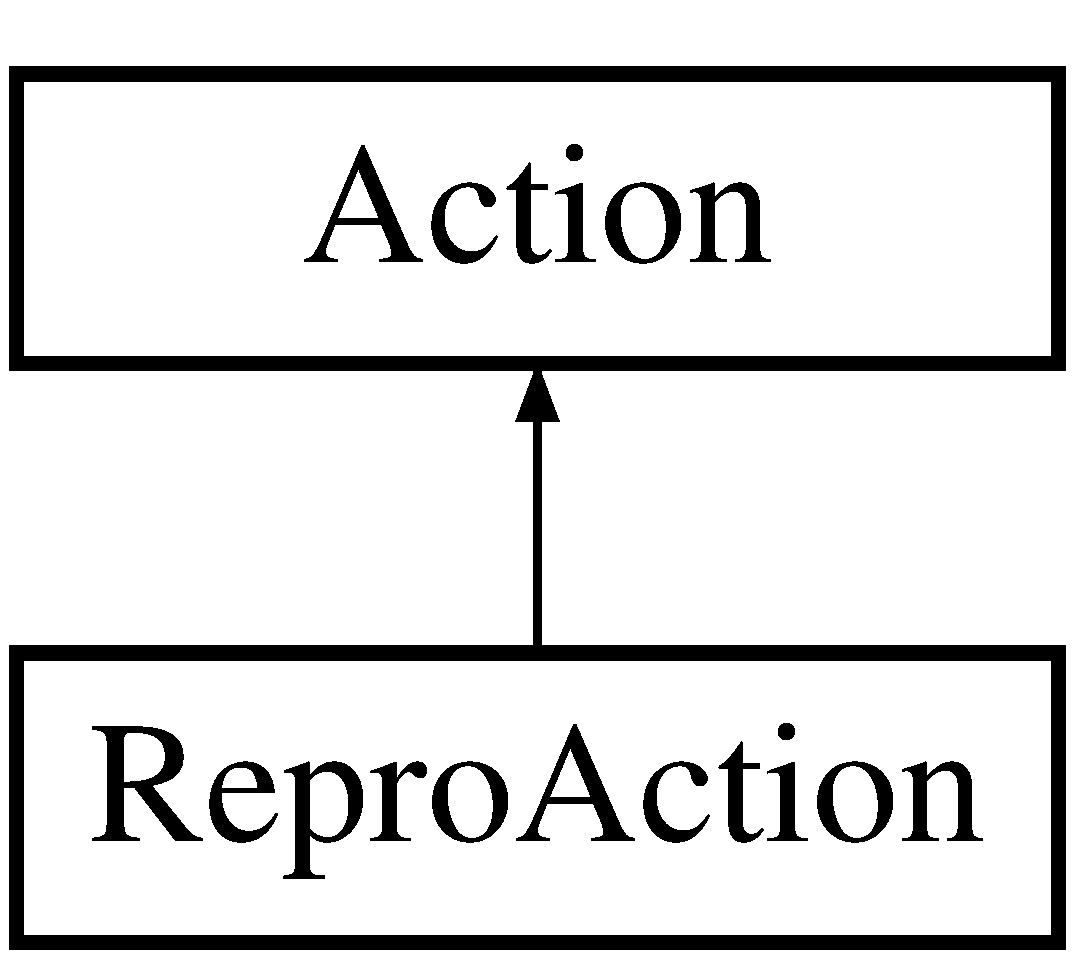
\includegraphics[height=2.000000cm]{class_repro_action}
\end{center}
\end{figure}
\subsection*{Public Member Functions}
\begin{DoxyCompactItemize}
\item 
override void \mbox{\hyperlink{class_repro_action_ab018325092d2a13cf333a8576c7f9dd0}{perform}} (\mbox{\hyperlink{class_creature}{Creature}} creature, \mbox{\hyperlink{class_ecosystem}{Ecosystem}} eco)
\item 
void \mbox{\hyperlink{class_repro_action_a0f1b2a6774238b935c3b2c544be7b5e0}{set\+Position}} (int\mbox{[}$\,$\mbox{]} parent\+Pos, int neighbor\+Index, int\mbox{[}$\,$\mbox{]} child\+Position)
\item 
\mbox{\hyperlink{class_repro_action}{Repro\+Action}} \mbox{\hyperlink{class_repro_action_ae68477b2e64171bf9a3bf20458fcc96c}{shallow\+Copy}} ()
\end{DoxyCompactItemize}
\subsection*{Additional Inherited Members}


\subsection{Member Function Documentation}
\mbox{\Hypertarget{class_repro_action_ab018325092d2a13cf333a8576c7f9dd0}\label{class_repro_action_ab018325092d2a13cf333a8576c7f9dd0}} 
\index{Repro\+Action@{Repro\+Action}!perform@{perform}}
\index{perform@{perform}!Repro\+Action@{Repro\+Action}}
\subsubsection{\texorpdfstring{perform()}{perform()}}
{\footnotesize\ttfamily override void Repro\+Action.\+perform (\begin{DoxyParamCaption}\item[{\mbox{\hyperlink{class_creature}{Creature}}}]{creature,  }\item[{\mbox{\hyperlink{class_ecosystem}{Ecosystem}}}]{eco }\end{DoxyParamCaption})\hspace{0.3cm}{\ttfamily [virtual]}}



Implements \mbox{\hyperlink{class_action_a2aedfc3be16448fbf224cb13607de3c0}{Action}}.

\mbox{\Hypertarget{class_repro_action_a0f1b2a6774238b935c3b2c544be7b5e0}\label{class_repro_action_a0f1b2a6774238b935c3b2c544be7b5e0}} 
\index{Repro\+Action@{Repro\+Action}!set\+Position@{set\+Position}}
\index{set\+Position@{set\+Position}!Repro\+Action@{Repro\+Action}}
\subsubsection{\texorpdfstring{set\+Position()}{setPosition()}}
{\footnotesize\ttfamily void Repro\+Action.\+set\+Position (\begin{DoxyParamCaption}\item[{int \mbox{[}$\,$\mbox{]}}]{parent\+Pos,  }\item[{int}]{neighbor\+Index,  }\item[{int \mbox{[}$\,$\mbox{]}}]{child\+Position }\end{DoxyParamCaption})}

\mbox{\Hypertarget{class_repro_action_ae68477b2e64171bf9a3bf20458fcc96c}\label{class_repro_action_ae68477b2e64171bf9a3bf20458fcc96c}} 
\index{Repro\+Action@{Repro\+Action}!shallow\+Copy@{shallow\+Copy}}
\index{shallow\+Copy@{shallow\+Copy}!Repro\+Action@{Repro\+Action}}
\subsubsection{\texorpdfstring{shallow\+Copy()}{shallowCopy()}}
{\footnotesize\ttfamily \mbox{\hyperlink{class_repro_action}{Repro\+Action}} Repro\+Action.\+shallow\+Copy (\begin{DoxyParamCaption}{ }\end{DoxyParamCaption})}



The documentation for this class was generated from the following file\+:\begin{DoxyCompactItemize}
\item 
\mbox{\hyperlink{_repro_action_8cs}{Repro\+Action.\+cs}}\end{DoxyCompactItemize}

\hypertarget{class_repro_action_editor}{}\section{Repro\+Action\+Editor Class Reference}
\label{class_repro_action_editor}\index{Repro\+Action\+Editor@{Repro\+Action\+Editor}}
Inheritance diagram for Repro\+Action\+Editor\+:\begin{figure}[H]
\begin{center}
\leavevmode
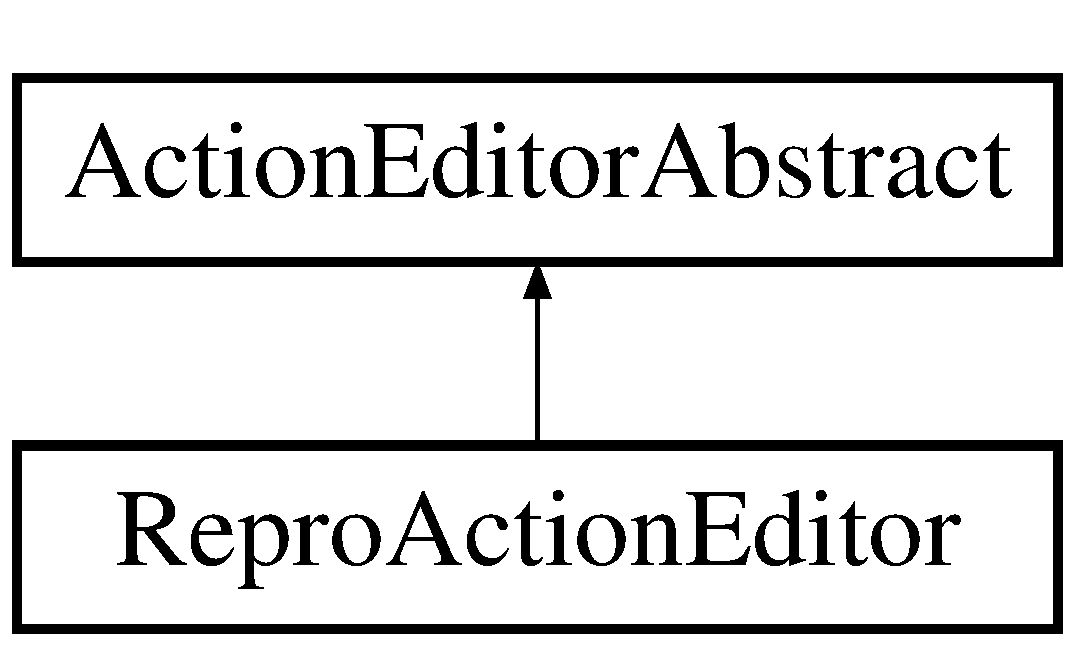
\includegraphics[height=2.000000cm]{class_repro_action_editor}
\end{center}
\end{figure}
\subsection*{Public Member Functions}
\begin{DoxyCompactItemize}
\item 
\mbox{\hyperlink{class_repro_action_editor_a8b70d2f53e4eb6224411021fc5ea3f33}{Repro\+Action\+Editor}} (\mbox{\hyperlink{class_repro_action}{Repro\+Action}} repro\+Action)
\end{DoxyCompactItemize}
\subsection*{Additional Inherited Members}


\subsection{Constructor \& Destructor Documentation}
\mbox{\Hypertarget{class_repro_action_editor_a8b70d2f53e4eb6224411021fc5ea3f33}\label{class_repro_action_editor_a8b70d2f53e4eb6224411021fc5ea3f33}} 
\index{Repro\+Action\+Editor@{Repro\+Action\+Editor}!Repro\+Action\+Editor@{Repro\+Action\+Editor}}
\index{Repro\+Action\+Editor@{Repro\+Action\+Editor}!Repro\+Action\+Editor@{Repro\+Action\+Editor}}
\subsubsection{\texorpdfstring{Repro\+Action\+Editor()}{ReproActionEditor()}}
{\footnotesize\ttfamily Repro\+Action\+Editor.\+Repro\+Action\+Editor (\begin{DoxyParamCaption}\item[{\mbox{\hyperlink{class_repro_action}{Repro\+Action}}}]{repro\+Action }\end{DoxyParamCaption})}



The documentation for this class was generated from the following file\+:\begin{DoxyCompactItemize}
\item 
\mbox{\hyperlink{_repro_action_editor_8cs}{Repro\+Action\+Editor.\+cs}}\end{DoxyCompactItemize}

\hypertarget{class_repro_network}{}\section{Repro\+Network Class Reference}
\label{class_repro_network}\index{Repro\+Network@{Repro\+Network}}


A specific kind of network that decided whether a creature should reproduce.  


Inheritance diagram for Repro\+Network\+:\begin{figure}[H]
\begin{center}
\leavevmode
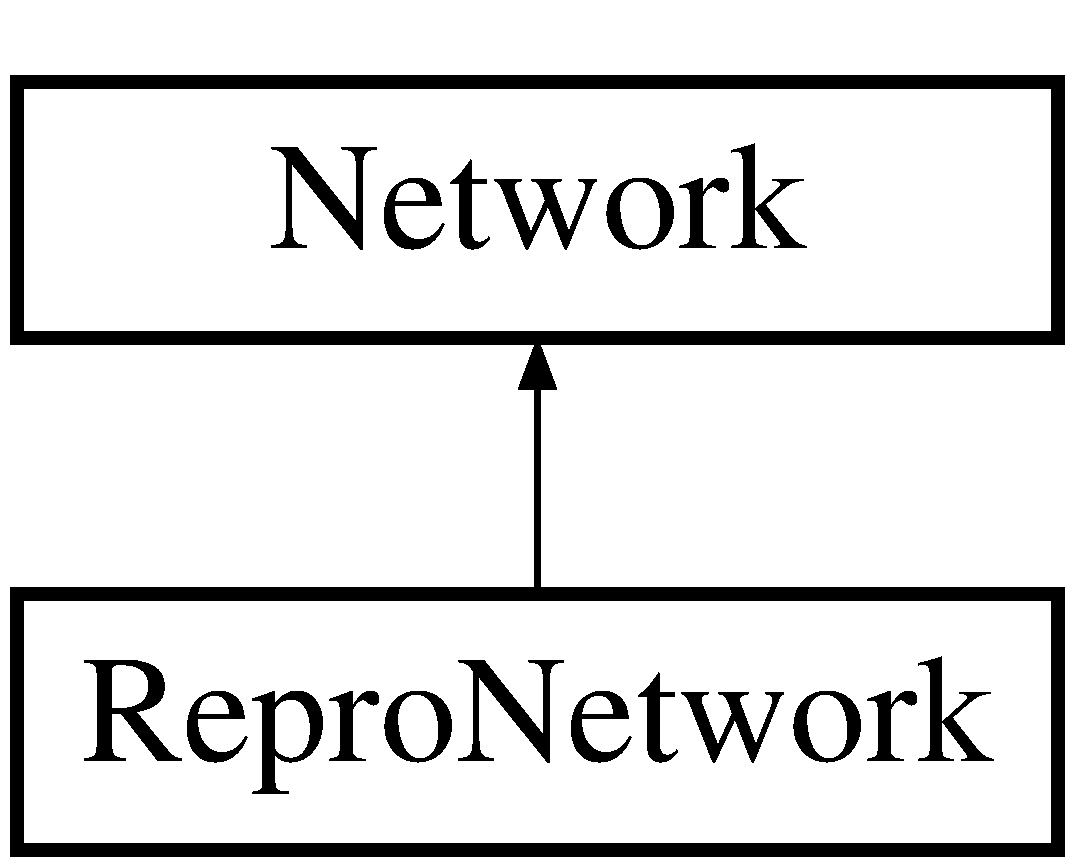
\includegraphics[height=2.000000cm]{class_repro_network}
\end{center}
\end{figure}
\subsection*{Public Attributes}
\begin{DoxyCompactItemize}
\item 
int \mbox{\hyperlink{class_repro_network_a2e648d1a88c94f1008a21c7c0d0b122b}{reproduce\+With}}
\begin{DoxyCompactList}\small\item\em Index of neighbor to reproduce with. \end{DoxyCompactList}\end{DoxyCompactItemize}
\subsection*{Additional Inherited Members}


\subsection{Detailed Description}
A specific kind of network that decided whether a creature should reproduce. 



\subsection{Member Data Documentation}
\mbox{\Hypertarget{class_repro_network_a2e648d1a88c94f1008a21c7c0d0b122b}\label{class_repro_network_a2e648d1a88c94f1008a21c7c0d0b122b}} 
\index{Repro\+Network@{Repro\+Network}!reproduce\+With@{reproduce\+With}}
\index{reproduce\+With@{reproduce\+With}!Repro\+Network@{Repro\+Network}}
\subsubsection{\texorpdfstring{reproduce\+With}{reproduceWith}}
{\footnotesize\ttfamily int Repro\+Network.\+reproduce\+With}



Index of neighbor to reproduce with. 



The documentation for this class was generated from the following file\+:\begin{DoxyCompactItemize}
\item 
\mbox{\hyperlink{_repro_network_8cs}{Repro\+Network.\+cs}}\end{DoxyCompactItemize}

\hypertarget{class_resource_editor}{}\section{Resource\+Editor Class Reference}
\label{class_resource_editor}\index{Resource\+Editor@{Resource\+Editor}}


A\+PI for setting resources that creature can store, and how the resource effects the creature.  


\subsection*{Public Member Functions}
\begin{DoxyCompactItemize}
\item 
\mbox{\hyperlink{class_resource_editor_a928faf6be8a59c7145e47948bcfeeeb2}{Resource\+Editor}} (\mbox{\hyperlink{class_creature_resource}{Creature\+Resource}} \+\_\+resource)
\item 
void \mbox{\hyperlink{class_resource_editor_a123d8260cfbc18a439e5e222ec1c101e}{set\+Level}} (float resource\+Level)
\item 
void \mbox{\hyperlink{class_resource_editor_a7b6f57a8791a396d56a2d08cea1db14b}{set\+Deficiency\+Health\+Drain}} (float drain\+Amt)
\begin{DoxyCompactList}\small\item\em Set amount of health drained per health\+Update when below deficiency threshold. \end{DoxyCompactList}\item 
void \mbox{\hyperlink{class_resource_editor_a98153dea69b0e350ae2ac75bf328891c}{set\+Deficiency\+Threshold}} (float deficiency\+Threshold)
\begin{DoxyCompactList}\small\item\em Set threshold at which deficiency occurs (health drain takes effect). \end{DoxyCompactList}\item 
void \mbox{\hyperlink{class_resource_editor_a4865f27f5f791455a7c4aa885be706a8}{set\+Health\+Gain}} (float health\+Gain)
\begin{DoxyCompactList}\small\item\em Set health gained when health gain threshold is met. \end{DoxyCompactList}\item 
void \mbox{\hyperlink{class_resource_editor_ac3d8fea68de6b8141fa6c777bb192590}{set\+Health\+Gain\+Threshold}} (float gain\+Threshold)
\begin{DoxyCompactList}\small\item\em Set threshold at which health is gained when it\textquotesingle{}s surpassed. \end{DoxyCompactList}\item 
void \mbox{\hyperlink{class_resource_editor_ac6807f97759768dfbf00a4517e46907d}{set\+Max\+Level}} (float max\+Level)
\item 
void \mbox{\hyperlink{class_resource_editor_afcd49279ce6e7d4c886dea66fcbe6d55}{set\+Base\+Usage}} (float base\+Usage)
\item 
void \mbox{\hyperlink{class_resource_editor_ae0558c83ceec579e083cf02d1a8e698e}{set\+Name}} (string name)
\end{DoxyCompactItemize}
\subsection*{Public Attributes}
\begin{DoxyCompactItemize}
\item 
\mbox{\hyperlink{class_creature_resource}{Creature\+Resource}} \mbox{\hyperlink{class_resource_editor_a523c5ec92b05df42505540a92df1e441}{resource}}
\begin{DoxyCompactList}\small\item\em Resource being created. \end{DoxyCompactList}\end{DoxyCompactItemize}


\subsection{Detailed Description}
A\+PI for setting resources that creature can store, and how the resource effects the creature. 



\subsection{Constructor \& Destructor Documentation}
\mbox{\Hypertarget{class_resource_editor_a928faf6be8a59c7145e47948bcfeeeb2}\label{class_resource_editor_a928faf6be8a59c7145e47948bcfeeeb2}} 
\index{Resource\+Editor@{Resource\+Editor}!Resource\+Editor@{Resource\+Editor}}
\index{Resource\+Editor@{Resource\+Editor}!Resource\+Editor@{Resource\+Editor}}
\subsubsection{\texorpdfstring{Resource\+Editor()}{ResourceEditor()}}
{\footnotesize\ttfamily Resource\+Editor.\+Resource\+Editor (\begin{DoxyParamCaption}\item[{\mbox{\hyperlink{class_creature_resource}{Creature\+Resource}}}]{\+\_\+resource }\end{DoxyParamCaption})}



\subsection{Member Function Documentation}
\mbox{\Hypertarget{class_resource_editor_afcd49279ce6e7d4c886dea66fcbe6d55}\label{class_resource_editor_afcd49279ce6e7d4c886dea66fcbe6d55}} 
\index{Resource\+Editor@{Resource\+Editor}!set\+Base\+Usage@{set\+Base\+Usage}}
\index{set\+Base\+Usage@{set\+Base\+Usage}!Resource\+Editor@{Resource\+Editor}}
\subsubsection{\texorpdfstring{set\+Base\+Usage()}{setBaseUsage()}}
{\footnotesize\ttfamily void Resource\+Editor.\+set\+Base\+Usage (\begin{DoxyParamCaption}\item[{float}]{base\+Usage }\end{DoxyParamCaption})}

\mbox{\Hypertarget{class_resource_editor_a7b6f57a8791a396d56a2d08cea1db14b}\label{class_resource_editor_a7b6f57a8791a396d56a2d08cea1db14b}} 
\index{Resource\+Editor@{Resource\+Editor}!set\+Deficiency\+Health\+Drain@{set\+Deficiency\+Health\+Drain}}
\index{set\+Deficiency\+Health\+Drain@{set\+Deficiency\+Health\+Drain}!Resource\+Editor@{Resource\+Editor}}
\subsubsection{\texorpdfstring{set\+Deficiency\+Health\+Drain()}{setDeficiencyHealthDrain()}}
{\footnotesize\ttfamily void Resource\+Editor.\+set\+Deficiency\+Health\+Drain (\begin{DoxyParamCaption}\item[{float}]{drain\+Amt }\end{DoxyParamCaption})}



Set amount of health drained per health\+Update when below deficiency threshold. 


\begin{DoxyParams}{Parameters}
{\em drain\+Amt} & Amount of health drained per health\+Update when below deficiency threshold.\\
\hline
\end{DoxyParams}
\mbox{\Hypertarget{class_resource_editor_a98153dea69b0e350ae2ac75bf328891c}\label{class_resource_editor_a98153dea69b0e350ae2ac75bf328891c}} 
\index{Resource\+Editor@{Resource\+Editor}!set\+Deficiency\+Threshold@{set\+Deficiency\+Threshold}}
\index{set\+Deficiency\+Threshold@{set\+Deficiency\+Threshold}!Resource\+Editor@{Resource\+Editor}}
\subsubsection{\texorpdfstring{set\+Deficiency\+Threshold()}{setDeficiencyThreshold()}}
{\footnotesize\ttfamily void Resource\+Editor.\+set\+Deficiency\+Threshold (\begin{DoxyParamCaption}\item[{float}]{deficiency\+Threshold }\end{DoxyParamCaption})}



Set threshold at which deficiency occurs (health drain takes effect). 


\begin{DoxyParams}{Parameters}
{\em deficiency\+Threshold} & Threshold at which deficiency occurs (health drain takes effect).\\
\hline
\end{DoxyParams}
\mbox{\Hypertarget{class_resource_editor_a4865f27f5f791455a7c4aa885be706a8}\label{class_resource_editor_a4865f27f5f791455a7c4aa885be706a8}} 
\index{Resource\+Editor@{Resource\+Editor}!set\+Health\+Gain@{set\+Health\+Gain}}
\index{set\+Health\+Gain@{set\+Health\+Gain}!Resource\+Editor@{Resource\+Editor}}
\subsubsection{\texorpdfstring{set\+Health\+Gain()}{setHealthGain()}}
{\footnotesize\ttfamily void Resource\+Editor.\+set\+Health\+Gain (\begin{DoxyParamCaption}\item[{float}]{health\+Gain }\end{DoxyParamCaption})}



Set health gained when health gain threshold is met. 


\begin{DoxyParams}{Parameters}
{\em health\+Gain} & Health gained when health gain threshold is met.\\
\hline
\end{DoxyParams}
\mbox{\Hypertarget{class_resource_editor_ac3d8fea68de6b8141fa6c777bb192590}\label{class_resource_editor_ac3d8fea68de6b8141fa6c777bb192590}} 
\index{Resource\+Editor@{Resource\+Editor}!set\+Health\+Gain\+Threshold@{set\+Health\+Gain\+Threshold}}
\index{set\+Health\+Gain\+Threshold@{set\+Health\+Gain\+Threshold}!Resource\+Editor@{Resource\+Editor}}
\subsubsection{\texorpdfstring{set\+Health\+Gain\+Threshold()}{setHealthGainThreshold()}}
{\footnotesize\ttfamily void Resource\+Editor.\+set\+Health\+Gain\+Threshold (\begin{DoxyParamCaption}\item[{float}]{gain\+Threshold }\end{DoxyParamCaption})}



Set threshold at which health is gained when it\textquotesingle{}s surpassed. 


\begin{DoxyParams}{Parameters}
{\em gain\+Threshold} & Threshold at which health is gained when it\textquotesingle{}s surpassed.\\
\hline
\end{DoxyParams}
\mbox{\Hypertarget{class_resource_editor_a123d8260cfbc18a439e5e222ec1c101e}\label{class_resource_editor_a123d8260cfbc18a439e5e222ec1c101e}} 
\index{Resource\+Editor@{Resource\+Editor}!set\+Level@{set\+Level}}
\index{set\+Level@{set\+Level}!Resource\+Editor@{Resource\+Editor}}
\subsubsection{\texorpdfstring{set\+Level()}{setLevel()}}
{\footnotesize\ttfamily void Resource\+Editor.\+set\+Level (\begin{DoxyParamCaption}\item[{float}]{resource\+Level }\end{DoxyParamCaption})}

\mbox{\Hypertarget{class_resource_editor_ac6807f97759768dfbf00a4517e46907d}\label{class_resource_editor_ac6807f97759768dfbf00a4517e46907d}} 
\index{Resource\+Editor@{Resource\+Editor}!set\+Max\+Level@{set\+Max\+Level}}
\index{set\+Max\+Level@{set\+Max\+Level}!Resource\+Editor@{Resource\+Editor}}
\subsubsection{\texorpdfstring{set\+Max\+Level()}{setMaxLevel()}}
{\footnotesize\ttfamily void Resource\+Editor.\+set\+Max\+Level (\begin{DoxyParamCaption}\item[{float}]{max\+Level }\end{DoxyParamCaption})}

\mbox{\Hypertarget{class_resource_editor_ae0558c83ceec579e083cf02d1a8e698e}\label{class_resource_editor_ae0558c83ceec579e083cf02d1a8e698e}} 
\index{Resource\+Editor@{Resource\+Editor}!set\+Name@{set\+Name}}
\index{set\+Name@{set\+Name}!Resource\+Editor@{Resource\+Editor}}
\subsubsection{\texorpdfstring{set\+Name()}{setName()}}
{\footnotesize\ttfamily void Resource\+Editor.\+set\+Name (\begin{DoxyParamCaption}\item[{string}]{name }\end{DoxyParamCaption})}



\subsection{Member Data Documentation}
\mbox{\Hypertarget{class_resource_editor_a523c5ec92b05df42505540a92df1e441}\label{class_resource_editor_a523c5ec92b05df42505540a92df1e441}} 
\index{Resource\+Editor@{Resource\+Editor}!resource@{resource}}
\index{resource@{resource}!Resource\+Editor@{Resource\+Editor}}
\subsubsection{\texorpdfstring{resource}{resource}}
{\footnotesize\ttfamily \mbox{\hyperlink{class_creature_resource}{Creature\+Resource}} Resource\+Editor.\+resource}



Resource being created. 



The documentation for this class was generated from the following file\+:\begin{DoxyCompactItemize}
\item 
\mbox{\hyperlink{_resource_editor_8cs}{Resource\+Editor.\+cs}}\end{DoxyCompactItemize}

\hypertarget{class_resource_store}{}\section{Resource\+Store Class Reference}
\label{class_resource_store}\index{Resource\+Store@{Resource\+Store}}


Basic unit of a resource to be stored in a \mbox{\hyperlink{class_land}{Land}} object. \mbox{\hyperlink{class_creature}{Creature}} can attempt to consume this resource from the land.  


\subsection*{Public Member Functions}
\begin{DoxyCompactItemize}
\item 
\mbox{\hyperlink{class_resource_store_aa9d9ff044e6156590656f1471b6d3e7d}{Resource\+Store}} (string \+\_\+name)
\item 
\mbox{\hyperlink{class_resource_store}{Resource\+Store}} \mbox{\hyperlink{class_resource_store_a7a609776888726de6169f1e9b90dd36f}{shallow\+Copy}} ()
\begin{DoxyCompactList}\small\item\em this returns a new instance of a resource store with shallow copies of all of the instance variables \end{DoxyCompactList}\item 
float \mbox{\hyperlink{class_resource_store_a0a779526593c2dab8e6b9d9e4d5013e6}{attempt\+Consumption}} (float time\+Dedicated, float creature\+Ability, float c\+Storage\+Space)
\begin{DoxyCompactList}\small\item\em Resolves amount of resource consumed in given amount of time. \end{DoxyCompactList}\item 
void \mbox{\hyperlink{class_resource_store_a9c37fdfe13469bed6232c3ed1418d313}{renew\+Resource}} ()
\begin{DoxyCompactList}\small\item\em Renews resource according to renewal\+Amt (called each time step). \end{DoxyCompactList}\item 
float \mbox{\hyperlink{class_resource_store_aa3b1414c69c413330e41fc53b32563ca}{get\+Proportion\+Stored}} ()
\end{DoxyCompactItemize}
\subsection*{Public Attributes}
\begin{DoxyCompactItemize}
\item 
float \mbox{\hyperlink{class_resource_store_a8fbddc12eb1ca75affdc31a4a5244917}{amount\+Stored}}
\begin{DoxyCompactList}\small\item\em Amount of resource stored. \end{DoxyCompactList}\item 
float \mbox{\hyperlink{class_resource_store_a17216b811a57c86dc3dfd0310f647bdb}{proportion\+Extracted}}
\begin{DoxyCompactList}\small\item\em Possible values\+: \mbox{[}0,1\mbox{]}. Proportion of the attempted amount that will be successfully extracted on one attempt. Modified by creature\textquotesingle{}s extraction ability. \end{DoxyCompactList}\item 
float \mbox{\hyperlink{class_resource_store_aadc1eae620b2c81bd4d16de13ca7f435}{amount\+Consumed\+Per\+Time\+Unit}}
\begin{DoxyCompactList}\small\item\em Amount of resource that can be taken by one action. \end{DoxyCompactList}\item 
float \mbox{\hyperlink{class_resource_store_a0f9723ce7385fb03909eeea64c38fdbb}{renewal\+Amt}}
\begin{DoxyCompactList}\small\item\em Amount renewed on a renewal step. \end{DoxyCompactList}\item 
string \mbox{\hyperlink{class_resource_store_a688e70d481b87077fd1af3c11743f9f8}{name}}
\item 
float \mbox{\hyperlink{class_resource_store_ae86f3cd5ac8a8bc58ee1db0917ef3021}{max\+Amount}}
\begin{DoxyCompactList}\small\item\em Maximum amount of resource that can be stored in this land location. \end{DoxyCompactList}\end{DoxyCompactItemize}


\subsection{Detailed Description}
Basic unit of a resource to be stored in a \mbox{\hyperlink{class_land}{Land}} object. \mbox{\hyperlink{class_creature}{Creature}} can attempt to consume this resource from the land. 



\subsection{Constructor \& Destructor Documentation}
\mbox{\Hypertarget{class_resource_store_aa9d9ff044e6156590656f1471b6d3e7d}\label{class_resource_store_aa9d9ff044e6156590656f1471b6d3e7d}} 
\index{Resource\+Store@{Resource\+Store}!Resource\+Store@{Resource\+Store}}
\index{Resource\+Store@{Resource\+Store}!Resource\+Store@{Resource\+Store}}
\subsubsection{\texorpdfstring{Resource\+Store()}{ResourceStore()}}
{\footnotesize\ttfamily Resource\+Store.\+Resource\+Store (\begin{DoxyParamCaption}\item[{string}]{\+\_\+name }\end{DoxyParamCaption})}



\subsection{Member Function Documentation}
\mbox{\Hypertarget{class_resource_store_a0a779526593c2dab8e6b9d9e4d5013e6}\label{class_resource_store_a0a779526593c2dab8e6b9d9e4d5013e6}} 
\index{Resource\+Store@{Resource\+Store}!attempt\+Consumption@{attempt\+Consumption}}
\index{attempt\+Consumption@{attempt\+Consumption}!Resource\+Store@{Resource\+Store}}
\subsubsection{\texorpdfstring{attempt\+Consumption()}{attemptConsumption()}}
{\footnotesize\ttfamily float Resource\+Store.\+attempt\+Consumption (\begin{DoxyParamCaption}\item[{float}]{time\+Dedicated,  }\item[{float}]{creature\+Ability,  }\item[{float}]{c\+Storage\+Space }\end{DoxyParamCaption})}



Resolves amount of resource consumed in given amount of time. 

\mbox{\Hypertarget{class_resource_store_aa3b1414c69c413330e41fc53b32563ca}\label{class_resource_store_aa3b1414c69c413330e41fc53b32563ca}} 
\index{Resource\+Store@{Resource\+Store}!get\+Proportion\+Stored@{get\+Proportion\+Stored}}
\index{get\+Proportion\+Stored@{get\+Proportion\+Stored}!Resource\+Store@{Resource\+Store}}
\subsubsection{\texorpdfstring{get\+Proportion\+Stored()}{getProportionStored()}}
{\footnotesize\ttfamily float Resource\+Store.\+get\+Proportion\+Stored (\begin{DoxyParamCaption}{ }\end{DoxyParamCaption})}

\mbox{\Hypertarget{class_resource_store_a9c37fdfe13469bed6232c3ed1418d313}\label{class_resource_store_a9c37fdfe13469bed6232c3ed1418d313}} 
\index{Resource\+Store@{Resource\+Store}!renew\+Resource@{renew\+Resource}}
\index{renew\+Resource@{renew\+Resource}!Resource\+Store@{Resource\+Store}}
\subsubsection{\texorpdfstring{renew\+Resource()}{renewResource()}}
{\footnotesize\ttfamily void Resource\+Store.\+renew\+Resource (\begin{DoxyParamCaption}{ }\end{DoxyParamCaption})}



Renews resource according to renewal\+Amt (called each time step). 

\mbox{\Hypertarget{class_resource_store_a7a609776888726de6169f1e9b90dd36f}\label{class_resource_store_a7a609776888726de6169f1e9b90dd36f}} 
\index{Resource\+Store@{Resource\+Store}!shallow\+Copy@{shallow\+Copy}}
\index{shallow\+Copy@{shallow\+Copy}!Resource\+Store@{Resource\+Store}}
\subsubsection{\texorpdfstring{shallow\+Copy()}{shallowCopy()}}
{\footnotesize\ttfamily \mbox{\hyperlink{class_resource_store}{Resource\+Store}} Resource\+Store.\+shallow\+Copy (\begin{DoxyParamCaption}{ }\end{DoxyParamCaption})}



this returns a new instance of a resource store with shallow copies of all of the instance variables 



\subsection{Member Data Documentation}
\mbox{\Hypertarget{class_resource_store_aadc1eae620b2c81bd4d16de13ca7f435}\label{class_resource_store_aadc1eae620b2c81bd4d16de13ca7f435}} 
\index{Resource\+Store@{Resource\+Store}!amount\+Consumed\+Per\+Time\+Unit@{amount\+Consumed\+Per\+Time\+Unit}}
\index{amount\+Consumed\+Per\+Time\+Unit@{amount\+Consumed\+Per\+Time\+Unit}!Resource\+Store@{Resource\+Store}}
\subsubsection{\texorpdfstring{amount\+Consumed\+Per\+Time\+Unit}{amountConsumedPerTimeUnit}}
{\footnotesize\ttfamily float Resource\+Store.\+amount\+Consumed\+Per\+Time\+Unit}



Amount of resource that can be taken by one action. 

\mbox{\Hypertarget{class_resource_store_a8fbddc12eb1ca75affdc31a4a5244917}\label{class_resource_store_a8fbddc12eb1ca75affdc31a4a5244917}} 
\index{Resource\+Store@{Resource\+Store}!amount\+Stored@{amount\+Stored}}
\index{amount\+Stored@{amount\+Stored}!Resource\+Store@{Resource\+Store}}
\subsubsection{\texorpdfstring{amount\+Stored}{amountStored}}
{\footnotesize\ttfamily float Resource\+Store.\+amount\+Stored}



Amount of resource stored. 

\mbox{\Hypertarget{class_resource_store_ae86f3cd5ac8a8bc58ee1db0917ef3021}\label{class_resource_store_ae86f3cd5ac8a8bc58ee1db0917ef3021}} 
\index{Resource\+Store@{Resource\+Store}!max\+Amount@{max\+Amount}}
\index{max\+Amount@{max\+Amount}!Resource\+Store@{Resource\+Store}}
\subsubsection{\texorpdfstring{max\+Amount}{maxAmount}}
{\footnotesize\ttfamily float Resource\+Store.\+max\+Amount}



Maximum amount of resource that can be stored in this land location. 

\mbox{\Hypertarget{class_resource_store_a688e70d481b87077fd1af3c11743f9f8}\label{class_resource_store_a688e70d481b87077fd1af3c11743f9f8}} 
\index{Resource\+Store@{Resource\+Store}!name@{name}}
\index{name@{name}!Resource\+Store@{Resource\+Store}}
\subsubsection{\texorpdfstring{name}{name}}
{\footnotesize\ttfamily string Resource\+Store.\+name}

\mbox{\Hypertarget{class_resource_store_a17216b811a57c86dc3dfd0310f647bdb}\label{class_resource_store_a17216b811a57c86dc3dfd0310f647bdb}} 
\index{Resource\+Store@{Resource\+Store}!proportion\+Extracted@{proportion\+Extracted}}
\index{proportion\+Extracted@{proportion\+Extracted}!Resource\+Store@{Resource\+Store}}
\subsubsection{\texorpdfstring{proportion\+Extracted}{proportionExtracted}}
{\footnotesize\ttfamily float Resource\+Store.\+proportion\+Extracted}



Possible values\+: \mbox{[}0,1\mbox{]}. Proportion of the attempted amount that will be successfully extracted on one attempt. Modified by creature\textquotesingle{}s extraction ability. 

\mbox{\Hypertarget{class_resource_store_a0f9723ce7385fb03909eeea64c38fdbb}\label{class_resource_store_a0f9723ce7385fb03909eeea64c38fdbb}} 
\index{Resource\+Store@{Resource\+Store}!renewal\+Amt@{renewal\+Amt}}
\index{renewal\+Amt@{renewal\+Amt}!Resource\+Store@{Resource\+Store}}
\subsubsection{\texorpdfstring{renewal\+Amt}{renewalAmt}}
{\footnotesize\ttfamily float Resource\+Store.\+renewal\+Amt}



Amount renewed on a renewal step. 



The documentation for this class was generated from the following file\+:\begin{DoxyCompactItemize}
\item 
\mbox{\hyperlink{_resource_store_8cs}{Resource\+Store.\+cs}}\end{DoxyCompactItemize}

\hypertarget{class_sensory_input_node}{}\section{Sensory\+Input\+Node Class Reference}
\label{class_sensory_input_node}\index{Sensory\+Input\+Node@{Sensory\+Input\+Node}}
Inheritance diagram for Sensory\+Input\+Node\+:\begin{figure}[H]
\begin{center}
\leavevmode
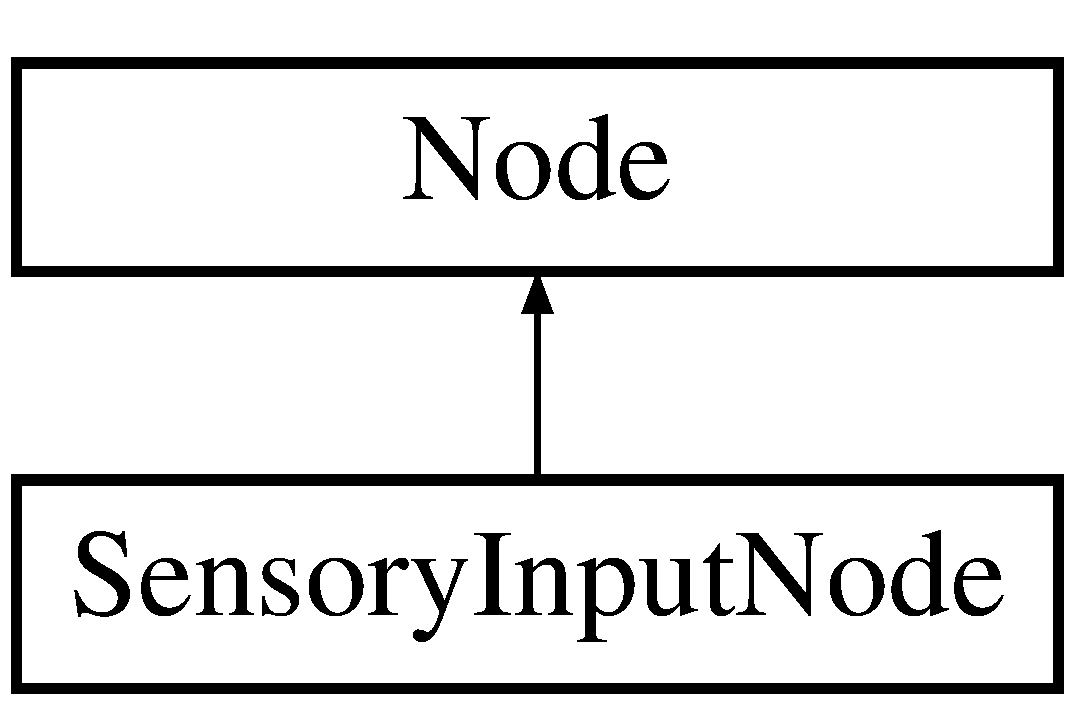
\includegraphics[height=2.000000cm]{class_sensory_input_node}
\end{center}
\end{figure}
\subsection*{Public Member Functions}
\begin{DoxyCompactItemize}
\item 
\mbox{\hyperlink{class_sensory_input_node_a45013c0e606dabbdeb51cdb12f56108d}{Sensory\+Input\+Node}} ()
\item 
\mbox{\hyperlink{class_sensory_input_node_a0af1e3930af4acd24155c7887fe38043}{Sensory\+Input\+Node}} (\mbox{\hyperlink{class_creature}{Creature}} \mbox{\hyperlink{class_sensory_input_node_a2886b0729565781d8e27cbfe72726625}{creature}})
\item 
void \mbox{\hyperlink{class_sensory_input_node_a31e18eb14cbeb233c8097e53b9f6c896}{set\+Creature}} (\mbox{\hyperlink{class_creature}{Creature}} parent\+Creature)
\item 
float \mbox{\hyperlink{class_sensory_input_node_a32f65537039b935585d204770eba89eb}{sense\+Val\+From\+Neighbor}} ()
\begin{DoxyCompactList}\small\item\em Uses neighbor\+Index and key with property\+Dict to get an updated value \end{DoxyCompactList}\item 
override void \mbox{\hyperlink{class_sensory_input_node_a3db8f13a203e1e604a3b79a20153cfa7}{update\+Value}} ()
\begin{DoxyCompactList}\small\item\em calls sense\+Val\+From\+Neighbor to update\+Value \end{DoxyCompactList}\item 
\mbox{\hyperlink{class_sensory_input_node}{Sensory\+Input\+Node}} \mbox{\hyperlink{class_sensory_input_node_afc439eb6875fbc26de67e4c546d1797c}{clone}} ()
\end{DoxyCompactItemize}
\subsection*{Public Attributes}
\begin{DoxyCompactItemize}
\item 
int \mbox{\hyperlink{class_sensory_input_node_aed52405e2e63c5e5ca6ad0142b3aaede}{neighbor\+Land\+Index}}
\begin{DoxyCompactList}\small\item\em specifies which neighbor \mbox{\hyperlink{class_land}{Land}} (0 -\/ 8) this node gets it\textquotesingle{}s input from\+: 0 for current\+Pos \end{DoxyCompactList}\item 
string \mbox{\hyperlink{class_sensory_input_node_a928c67bebc7f59466c91cbc6c5552bb4}{sensed\+Resource}}
\begin{DoxyCompactList}\small\item\em string designating resource to be found in neighbor dictionary \end{DoxyCompactList}\item 
\mbox{\hyperlink{class_creature}{Creature}} \mbox{\hyperlink{class_sensory_input_node_a2886b0729565781d8e27cbfe72726625}{creature}}
\begin{DoxyCompactList}\small\item\em stores a reference to the creature it belongs to (for getting neighbors) \end{DoxyCompactList}\end{DoxyCompactItemize}


\subsection{Constructor \& Destructor Documentation}
\mbox{\Hypertarget{class_sensory_input_node_a45013c0e606dabbdeb51cdb12f56108d}\label{class_sensory_input_node_a45013c0e606dabbdeb51cdb12f56108d}} 
\index{Sensory\+Input\+Node@{Sensory\+Input\+Node}!Sensory\+Input\+Node@{Sensory\+Input\+Node}}
\index{Sensory\+Input\+Node@{Sensory\+Input\+Node}!Sensory\+Input\+Node@{Sensory\+Input\+Node}}
\subsubsection{\texorpdfstring{Sensory\+Input\+Node()}{SensoryInputNode()}\hspace{0.1cm}{\footnotesize\ttfamily [1/2]}}
{\footnotesize\ttfamily Sensory\+Input\+Node.\+Sensory\+Input\+Node (\begin{DoxyParamCaption}{ }\end{DoxyParamCaption})}

\mbox{\Hypertarget{class_sensory_input_node_a0af1e3930af4acd24155c7887fe38043}\label{class_sensory_input_node_a0af1e3930af4acd24155c7887fe38043}} 
\index{Sensory\+Input\+Node@{Sensory\+Input\+Node}!Sensory\+Input\+Node@{Sensory\+Input\+Node}}
\index{Sensory\+Input\+Node@{Sensory\+Input\+Node}!Sensory\+Input\+Node@{Sensory\+Input\+Node}}
\subsubsection{\texorpdfstring{Sensory\+Input\+Node()}{SensoryInputNode()}\hspace{0.1cm}{\footnotesize\ttfamily [2/2]}}
{\footnotesize\ttfamily Sensory\+Input\+Node.\+Sensory\+Input\+Node (\begin{DoxyParamCaption}\item[{\mbox{\hyperlink{class_creature}{Creature}}}]{creature }\end{DoxyParamCaption})}



\subsection{Member Function Documentation}
\mbox{\Hypertarget{class_sensory_input_node_afc439eb6875fbc26de67e4c546d1797c}\label{class_sensory_input_node_afc439eb6875fbc26de67e4c546d1797c}} 
\index{Sensory\+Input\+Node@{Sensory\+Input\+Node}!clone@{clone}}
\index{clone@{clone}!Sensory\+Input\+Node@{Sensory\+Input\+Node}}
\subsubsection{\texorpdfstring{clone()}{clone()}}
{\footnotesize\ttfamily \mbox{\hyperlink{class_sensory_input_node}{Sensory\+Input\+Node}} Sensory\+Input\+Node.\+clone (\begin{DoxyParamCaption}{ }\end{DoxyParamCaption})}

\mbox{\Hypertarget{class_sensory_input_node_a32f65537039b935585d204770eba89eb}\label{class_sensory_input_node_a32f65537039b935585d204770eba89eb}} 
\index{Sensory\+Input\+Node@{Sensory\+Input\+Node}!sense\+Val\+From\+Neighbor@{sense\+Val\+From\+Neighbor}}
\index{sense\+Val\+From\+Neighbor@{sense\+Val\+From\+Neighbor}!Sensory\+Input\+Node@{Sensory\+Input\+Node}}
\subsubsection{\texorpdfstring{sense\+Val\+From\+Neighbor()}{senseValFromNeighbor()}}
{\footnotesize\ttfamily float Sensory\+Input\+Node.\+sense\+Val\+From\+Neighbor (\begin{DoxyParamCaption}{ }\end{DoxyParamCaption})}



Uses neighbor\+Index and key with property\+Dict to get an updated value 

\mbox{\Hypertarget{class_sensory_input_node_a31e18eb14cbeb233c8097e53b9f6c896}\label{class_sensory_input_node_a31e18eb14cbeb233c8097e53b9f6c896}} 
\index{Sensory\+Input\+Node@{Sensory\+Input\+Node}!set\+Creature@{set\+Creature}}
\index{set\+Creature@{set\+Creature}!Sensory\+Input\+Node@{Sensory\+Input\+Node}}
\subsubsection{\texorpdfstring{set\+Creature()}{setCreature()}}
{\footnotesize\ttfamily void Sensory\+Input\+Node.\+set\+Creature (\begin{DoxyParamCaption}\item[{\mbox{\hyperlink{class_creature}{Creature}}}]{parent\+Creature }\end{DoxyParamCaption})}

\mbox{\Hypertarget{class_sensory_input_node_a3db8f13a203e1e604a3b79a20153cfa7}\label{class_sensory_input_node_a3db8f13a203e1e604a3b79a20153cfa7}} 
\index{Sensory\+Input\+Node@{Sensory\+Input\+Node}!update\+Value@{update\+Value}}
\index{update\+Value@{update\+Value}!Sensory\+Input\+Node@{Sensory\+Input\+Node}}
\subsubsection{\texorpdfstring{update\+Value()}{updateValue()}}
{\footnotesize\ttfamily override void Sensory\+Input\+Node.\+update\+Value (\begin{DoxyParamCaption}{ }\end{DoxyParamCaption})\hspace{0.3cm}{\ttfamily [virtual]}}



calls sense\+Val\+From\+Neighbor to update\+Value 



Implements \mbox{\hyperlink{class_node_a85ebd0e36c25430570b94f923afd2a62}{Node}}.



\subsection{Member Data Documentation}
\mbox{\Hypertarget{class_sensory_input_node_a2886b0729565781d8e27cbfe72726625}\label{class_sensory_input_node_a2886b0729565781d8e27cbfe72726625}} 
\index{Sensory\+Input\+Node@{Sensory\+Input\+Node}!creature@{creature}}
\index{creature@{creature}!Sensory\+Input\+Node@{Sensory\+Input\+Node}}
\subsubsection{\texorpdfstring{creature}{creature}}
{\footnotesize\ttfamily \mbox{\hyperlink{class_creature}{Creature}} Sensory\+Input\+Node.\+creature}



stores a reference to the creature it belongs to (for getting neighbors) 

\mbox{\Hypertarget{class_sensory_input_node_aed52405e2e63c5e5ca6ad0142b3aaede}\label{class_sensory_input_node_aed52405e2e63c5e5ca6ad0142b3aaede}} 
\index{Sensory\+Input\+Node@{Sensory\+Input\+Node}!neighbor\+Land\+Index@{neighbor\+Land\+Index}}
\index{neighbor\+Land\+Index@{neighbor\+Land\+Index}!Sensory\+Input\+Node@{Sensory\+Input\+Node}}
\subsubsection{\texorpdfstring{neighbor\+Land\+Index}{neighborLandIndex}}
{\footnotesize\ttfamily int Sensory\+Input\+Node.\+neighbor\+Land\+Index}



specifies which neighbor \mbox{\hyperlink{class_land}{Land}} (0 -\/ 8) this node gets it\textquotesingle{}s input from\+: 0 for current\+Pos 

\mbox{\Hypertarget{class_sensory_input_node_a928c67bebc7f59466c91cbc6c5552bb4}\label{class_sensory_input_node_a928c67bebc7f59466c91cbc6c5552bb4}} 
\index{Sensory\+Input\+Node@{Sensory\+Input\+Node}!sensed\+Resource@{sensed\+Resource}}
\index{sensed\+Resource@{sensed\+Resource}!Sensory\+Input\+Node@{Sensory\+Input\+Node}}
\subsubsection{\texorpdfstring{sensed\+Resource}{sensedResource}}
{\footnotesize\ttfamily string Sensory\+Input\+Node.\+sensed\+Resource}



string designating resource to be found in neighbor dictionary 



The documentation for this class was generated from the following file\+:\begin{DoxyCompactItemize}
\item 
\mbox{\hyperlink{_sensory_input_node_8cs}{Sensory\+Input\+Node.\+cs}}\end{DoxyCompactItemize}

\hypertarget{class_sensory_input_node_editor}{}\section{Sensory\+Input\+Node\+Editor Class Reference}
\label{class_sensory_input_node_editor}\index{Sensory\+Input\+Node\+Editor@{Sensory\+Input\+Node\+Editor}}


A\+PI for Sensory\+Input\+Nodes.  


Inheritance diagram for Sensory\+Input\+Node\+Editor\+:\begin{figure}[H]
\begin{center}
\leavevmode
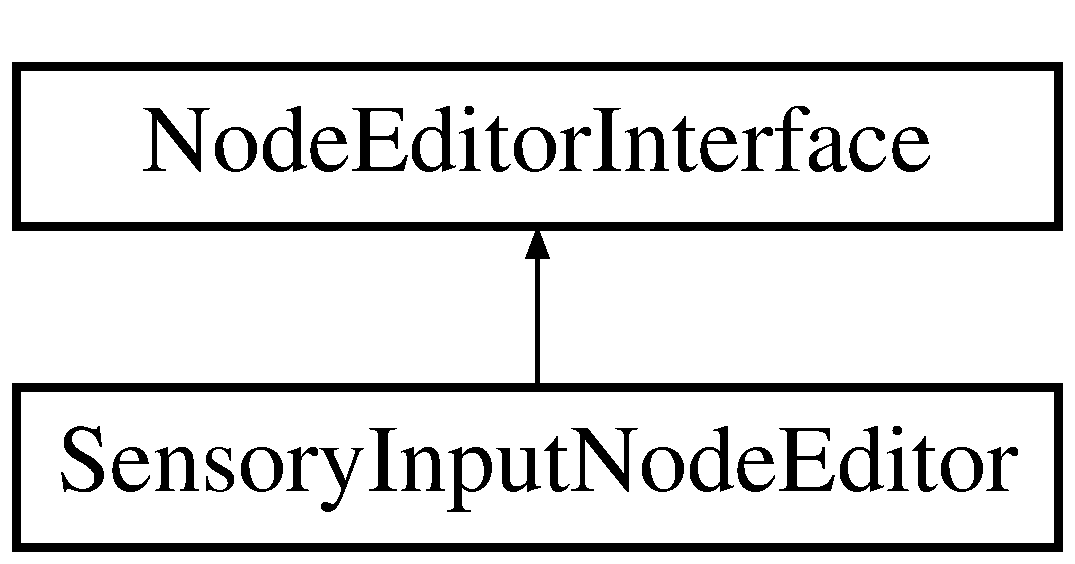
\includegraphics[height=2.000000cm]{class_sensory_input_node_editor}
\end{center}
\end{figure}
\subsection*{Public Member Functions}
\begin{DoxyCompactItemize}
\item 
\mbox{\hyperlink{class_sensory_input_node_editor_aa2b8400dc6ba926026c2580ed83fdc25}{Sensory\+Input\+Node\+Editor}} (\mbox{\hyperlink{class_sensory_input_node}{Sensory\+Input\+Node}} \+\_\+si\+Node, int \+\_\+node\+Layer)
\item 
\mbox{\hyperlink{class_node}{Node}} \mbox{\hyperlink{class_sensory_input_node_editor_ab6f6a94004254d8bba213a6e91fcc946}{get\+Node}} ()
\item 
void \mbox{\hyperlink{class_sensory_input_node_editor_a6c8e83c4bf895984f57f712f1fad1dcb}{set\+Land\+Index}} (int index)
\item 
void \mbox{\hyperlink{class_sensory_input_node_editor_a6441e77cda6614c60aeac8585acd2b4e}{set\+Sensed\+Resource}} (string resource)
\end{DoxyCompactItemize}
\subsection*{Public Attributes}
\begin{DoxyCompactItemize}
\item 
\mbox{\hyperlink{class_sensory_input_node}{Sensory\+Input\+Node}} \mbox{\hyperlink{class_sensory_input_node_editor_a276780a449128bccbae7730ef816f6db}{si\+Node}}
\item 
int \mbox{\hyperlink{class_sensory_input_node_editor_a22f4c25856b251e847ad8ac4d90351bf}{node\+Layer}}
\end{DoxyCompactItemize}


\subsection{Detailed Description}
A\+PI for Sensory\+Input\+Nodes. 



\subsection{Constructor \& Destructor Documentation}
\mbox{\Hypertarget{class_sensory_input_node_editor_aa2b8400dc6ba926026c2580ed83fdc25}\label{class_sensory_input_node_editor_aa2b8400dc6ba926026c2580ed83fdc25}} 
\index{Sensory\+Input\+Node\+Editor@{Sensory\+Input\+Node\+Editor}!Sensory\+Input\+Node\+Editor@{Sensory\+Input\+Node\+Editor}}
\index{Sensory\+Input\+Node\+Editor@{Sensory\+Input\+Node\+Editor}!Sensory\+Input\+Node\+Editor@{Sensory\+Input\+Node\+Editor}}
\subsubsection{\texorpdfstring{Sensory\+Input\+Node\+Editor()}{SensoryInputNodeEditor()}}
{\footnotesize\ttfamily Sensory\+Input\+Node\+Editor.\+Sensory\+Input\+Node\+Editor (\begin{DoxyParamCaption}\item[{\mbox{\hyperlink{class_sensory_input_node}{Sensory\+Input\+Node}}}]{\+\_\+si\+Node,  }\item[{int}]{\+\_\+node\+Layer }\end{DoxyParamCaption})}



\subsection{Member Function Documentation}
\mbox{\Hypertarget{class_sensory_input_node_editor_ab6f6a94004254d8bba213a6e91fcc946}\label{class_sensory_input_node_editor_ab6f6a94004254d8bba213a6e91fcc946}} 
\index{Sensory\+Input\+Node\+Editor@{Sensory\+Input\+Node\+Editor}!get\+Node@{get\+Node}}
\index{get\+Node@{get\+Node}!Sensory\+Input\+Node\+Editor@{Sensory\+Input\+Node\+Editor}}
\subsubsection{\texorpdfstring{get\+Node()}{getNode()}}
{\footnotesize\ttfamily \mbox{\hyperlink{class_node}{Node}} Sensory\+Input\+Node\+Editor.\+get\+Node (\begin{DoxyParamCaption}{ }\end{DoxyParamCaption})}



Implements \mbox{\hyperlink{interface_node_editor_interface_a56e2abaedf17d7fbf2be90d521ec9363}{Node\+Editor\+Interface}}.

\mbox{\Hypertarget{class_sensory_input_node_editor_a6c8e83c4bf895984f57f712f1fad1dcb}\label{class_sensory_input_node_editor_a6c8e83c4bf895984f57f712f1fad1dcb}} 
\index{Sensory\+Input\+Node\+Editor@{Sensory\+Input\+Node\+Editor}!set\+Land\+Index@{set\+Land\+Index}}
\index{set\+Land\+Index@{set\+Land\+Index}!Sensory\+Input\+Node\+Editor@{Sensory\+Input\+Node\+Editor}}
\subsubsection{\texorpdfstring{set\+Land\+Index()}{setLandIndex()}}
{\footnotesize\ttfamily void Sensory\+Input\+Node\+Editor.\+set\+Land\+Index (\begin{DoxyParamCaption}\item[{int}]{index }\end{DoxyParamCaption})}

\mbox{\Hypertarget{class_sensory_input_node_editor_a6441e77cda6614c60aeac8585acd2b4e}\label{class_sensory_input_node_editor_a6441e77cda6614c60aeac8585acd2b4e}} 
\index{Sensory\+Input\+Node\+Editor@{Sensory\+Input\+Node\+Editor}!set\+Sensed\+Resource@{set\+Sensed\+Resource}}
\index{set\+Sensed\+Resource@{set\+Sensed\+Resource}!Sensory\+Input\+Node\+Editor@{Sensory\+Input\+Node\+Editor}}
\subsubsection{\texorpdfstring{set\+Sensed\+Resource()}{setSensedResource()}}
{\footnotesize\ttfamily void Sensory\+Input\+Node\+Editor.\+set\+Sensed\+Resource (\begin{DoxyParamCaption}\item[{string}]{resource }\end{DoxyParamCaption})}



\subsection{Member Data Documentation}
\mbox{\Hypertarget{class_sensory_input_node_editor_a22f4c25856b251e847ad8ac4d90351bf}\label{class_sensory_input_node_editor_a22f4c25856b251e847ad8ac4d90351bf}} 
\index{Sensory\+Input\+Node\+Editor@{Sensory\+Input\+Node\+Editor}!node\+Layer@{node\+Layer}}
\index{node\+Layer@{node\+Layer}!Sensory\+Input\+Node\+Editor@{Sensory\+Input\+Node\+Editor}}
\subsubsection{\texorpdfstring{node\+Layer}{nodeLayer}}
{\footnotesize\ttfamily int Sensory\+Input\+Node\+Editor.\+node\+Layer}

\mbox{\Hypertarget{class_sensory_input_node_editor_a276780a449128bccbae7730ef816f6db}\label{class_sensory_input_node_editor_a276780a449128bccbae7730ef816f6db}} 
\index{Sensory\+Input\+Node\+Editor@{Sensory\+Input\+Node\+Editor}!si\+Node@{si\+Node}}
\index{si\+Node@{si\+Node}!Sensory\+Input\+Node\+Editor@{Sensory\+Input\+Node\+Editor}}
\subsubsection{\texorpdfstring{si\+Node}{siNode}}
{\footnotesize\ttfamily \mbox{\hyperlink{class_sensory_input_node}{Sensory\+Input\+Node}} Sensory\+Input\+Node\+Editor.\+si\+Node}



The documentation for this class was generated from the following file\+:\begin{DoxyCompactItemize}
\item 
\mbox{\hyperlink{_sensory_input_node_editor_8cs}{Sensory\+Input\+Node\+Editor.\+cs}}\end{DoxyCompactItemize}

\hypertarget{class_sim_runner_test}{}\section{Sim\+Runner\+Test Class Reference}
\label{class_sim_runner_test}\index{Sim\+Runner\+Test@{Sim\+Runner\+Test}}


Class for running simulation.  


Inheritance diagram for Sim\+Runner\+Test\+:\begin{figure}[H]
\begin{center}
\leavevmode
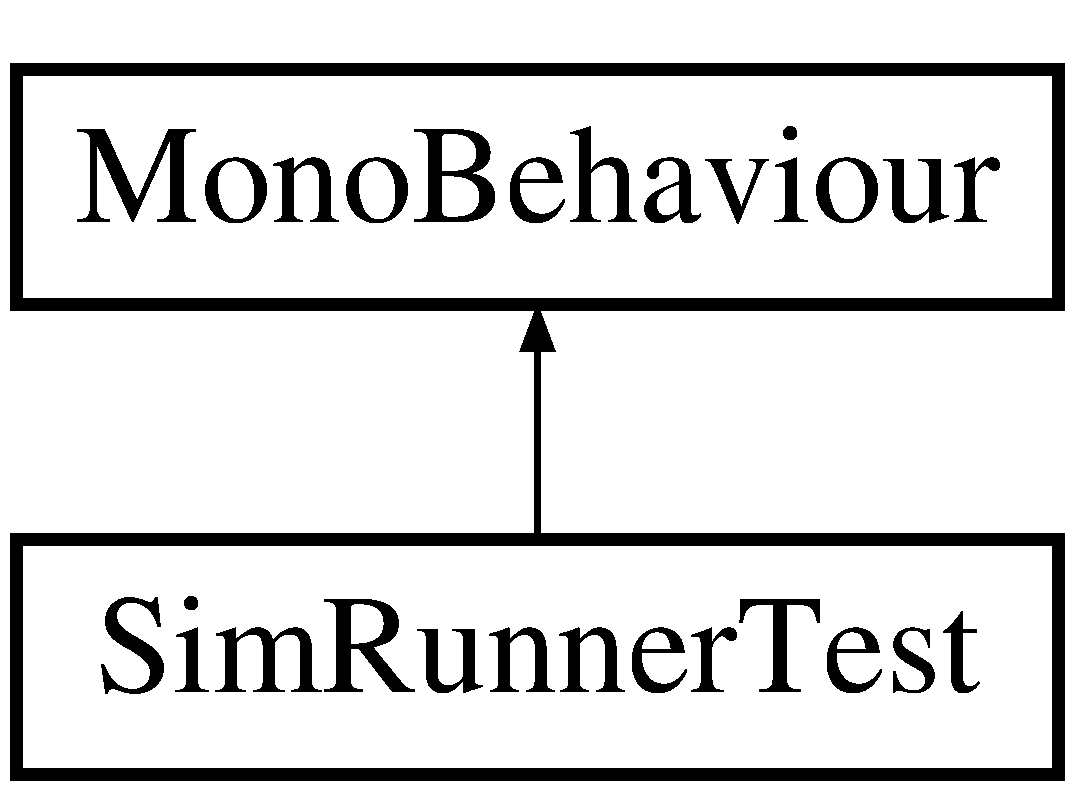
\includegraphics[height=2.000000cm]{class_sim_runner_test}
\end{center}
\end{figure}
\subsection*{Public Member Functions}
\begin{DoxyCompactItemize}
\item 
void \mbox{\hyperlink{class_sim_runner_test_a2c0a21b60ed966ab67b2bdf46e4b4b4e}{flip\+Paused}} ()
\item 
void \mbox{\hyperlink{class_sim_runner_test_ae48ceacccbc52ef5a7f037f0a723a781}{set\+Steps}} ()
\item 
void \mbox{\hyperlink{class_sim_runner_test_a7919c296008d4ed412b1b6c1469753ef}{get\+Val\+From\+Slider}} (float value)
\end{DoxyCompactItemize}
\subsection*{Public Attributes}
\begin{DoxyCompactItemize}
\item 
Game\+Object \mbox{\hyperlink{class_sim_runner_test_a630ab4bd41cddc58b193d990f8ae225b}{tile\+Prefab}}
\item 
Game\+Object \mbox{\hyperlink{class_sim_runner_test_a6b09f48590c46e807abe6d551b17dda0}{steps\+Text}}
\item 
Game\+Object \mbox{\hyperlink{class_sim_runner_test_aa6c06d9cb1c9bf367315315202abbae7}{map\+Sprite\+Obj}}
\end{DoxyCompactItemize}


\subsection{Detailed Description}
Class for running simulation. 



\subsection{Member Function Documentation}
\mbox{\Hypertarget{class_sim_runner_test_a2c0a21b60ed966ab67b2bdf46e4b4b4e}\label{class_sim_runner_test_a2c0a21b60ed966ab67b2bdf46e4b4b4e}} 
\index{Sim\+Runner\+Test@{Sim\+Runner\+Test}!flip\+Paused@{flip\+Paused}}
\index{flip\+Paused@{flip\+Paused}!Sim\+Runner\+Test@{Sim\+Runner\+Test}}
\subsubsection{\texorpdfstring{flip\+Paused()}{flipPaused()}}
{\footnotesize\ttfamily void Sim\+Runner\+Test.\+flip\+Paused (\begin{DoxyParamCaption}{ }\end{DoxyParamCaption})}

\mbox{\Hypertarget{class_sim_runner_test_a7919c296008d4ed412b1b6c1469753ef}\label{class_sim_runner_test_a7919c296008d4ed412b1b6c1469753ef}} 
\index{Sim\+Runner\+Test@{Sim\+Runner\+Test}!get\+Val\+From\+Slider@{get\+Val\+From\+Slider}}
\index{get\+Val\+From\+Slider@{get\+Val\+From\+Slider}!Sim\+Runner\+Test@{Sim\+Runner\+Test}}
\subsubsection{\texorpdfstring{get\+Val\+From\+Slider()}{getValFromSlider()}}
{\footnotesize\ttfamily void Sim\+Runner\+Test.\+get\+Val\+From\+Slider (\begin{DoxyParamCaption}\item[{float}]{value }\end{DoxyParamCaption})}

\mbox{\Hypertarget{class_sim_runner_test_ae48ceacccbc52ef5a7f037f0a723a781}\label{class_sim_runner_test_ae48ceacccbc52ef5a7f037f0a723a781}} 
\index{Sim\+Runner\+Test@{Sim\+Runner\+Test}!set\+Steps@{set\+Steps}}
\index{set\+Steps@{set\+Steps}!Sim\+Runner\+Test@{Sim\+Runner\+Test}}
\subsubsection{\texorpdfstring{set\+Steps()}{setSteps()}}
{\footnotesize\ttfamily void Sim\+Runner\+Test.\+set\+Steps (\begin{DoxyParamCaption}{ }\end{DoxyParamCaption})}



\subsection{Member Data Documentation}
\mbox{\Hypertarget{class_sim_runner_test_aa6c06d9cb1c9bf367315315202abbae7}\label{class_sim_runner_test_aa6c06d9cb1c9bf367315315202abbae7}} 
\index{Sim\+Runner\+Test@{Sim\+Runner\+Test}!map\+Sprite\+Obj@{map\+Sprite\+Obj}}
\index{map\+Sprite\+Obj@{map\+Sprite\+Obj}!Sim\+Runner\+Test@{Sim\+Runner\+Test}}
\subsubsection{\texorpdfstring{map\+Sprite\+Obj}{mapSpriteObj}}
{\footnotesize\ttfamily Game\+Object Sim\+Runner\+Test.\+map\+Sprite\+Obj}

\mbox{\Hypertarget{class_sim_runner_test_a6b09f48590c46e807abe6d551b17dda0}\label{class_sim_runner_test_a6b09f48590c46e807abe6d551b17dda0}} 
\index{Sim\+Runner\+Test@{Sim\+Runner\+Test}!steps\+Text@{steps\+Text}}
\index{steps\+Text@{steps\+Text}!Sim\+Runner\+Test@{Sim\+Runner\+Test}}
\subsubsection{\texorpdfstring{steps\+Text}{stepsText}}
{\footnotesize\ttfamily Game\+Object Sim\+Runner\+Test.\+steps\+Text}

\mbox{\Hypertarget{class_sim_runner_test_a630ab4bd41cddc58b193d990f8ae225b}\label{class_sim_runner_test_a630ab4bd41cddc58b193d990f8ae225b}} 
\index{Sim\+Runner\+Test@{Sim\+Runner\+Test}!tile\+Prefab@{tile\+Prefab}}
\index{tile\+Prefab@{tile\+Prefab}!Sim\+Runner\+Test@{Sim\+Runner\+Test}}
\subsubsection{\texorpdfstring{tile\+Prefab}{tilePrefab}}
{\footnotesize\ttfamily Game\+Object Sim\+Runner\+Test.\+tile\+Prefab}



The documentation for this class was generated from the following file\+:\begin{DoxyCompactItemize}
\item 
\mbox{\hyperlink{_sim_runner_test_8cs}{Sim\+Runner\+Test.\+cs}}\end{DoxyCompactItemize}

\hypertarget{class_sim_runner_user}{}\section{Sim\+Runner\+User Class Reference}
\label{class_sim_runner_user}\index{Sim\+Runner\+User@{Sim\+Runner\+User}}


Class for running simulation.  


Inheritance diagram for Sim\+Runner\+User\+:\begin{figure}[H]
\begin{center}
\leavevmode
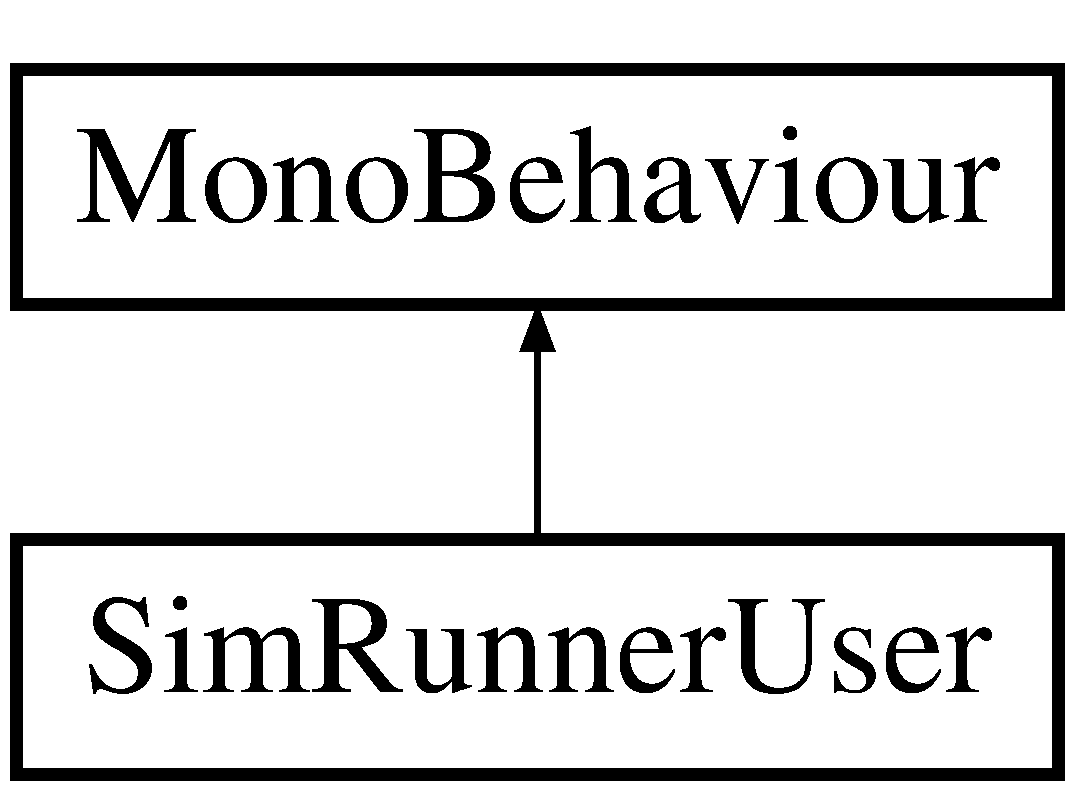
\includegraphics[height=2.000000cm]{class_sim_runner_user}
\end{center}
\end{figure}
\subsection*{Public Member Functions}
\begin{DoxyCompactItemize}
\item 
void \mbox{\hyperlink{class_sim_runner_user_a8e0173173b2f5dc76cd4f280f9978897}{start\+Sim}} (int interval)
\end{DoxyCompactItemize}
\subsection*{Public Attributes}
\begin{DoxyCompactItemize}
\item 
Game\+Object \mbox{\hyperlink{class_sim_runner_user_a049fcb968076857e64527f1ed6645284}{tile\+Prefab}}
\end{DoxyCompactItemize}


\subsection{Detailed Description}
Class for running simulation. 



\subsection{Member Function Documentation}
\mbox{\Hypertarget{class_sim_runner_user_a8e0173173b2f5dc76cd4f280f9978897}\label{class_sim_runner_user_a8e0173173b2f5dc76cd4f280f9978897}} 
\index{Sim\+Runner\+User@{Sim\+Runner\+User}!start\+Sim@{start\+Sim}}
\index{start\+Sim@{start\+Sim}!Sim\+Runner\+User@{Sim\+Runner\+User}}
\subsubsection{\texorpdfstring{start\+Sim()}{startSim()}}
{\footnotesize\ttfamily void Sim\+Runner\+User.\+start\+Sim (\begin{DoxyParamCaption}\item[{int}]{interval }\end{DoxyParamCaption})}



\subsection{Member Data Documentation}
\mbox{\Hypertarget{class_sim_runner_user_a049fcb968076857e64527f1ed6645284}\label{class_sim_runner_user_a049fcb968076857e64527f1ed6645284}} 
\index{Sim\+Runner\+User@{Sim\+Runner\+User}!tile\+Prefab@{tile\+Prefab}}
\index{tile\+Prefab@{tile\+Prefab}!Sim\+Runner\+User@{Sim\+Runner\+User}}
\subsubsection{\texorpdfstring{tile\+Prefab}{tilePrefab}}
{\footnotesize\ttfamily Game\+Object Sim\+Runner\+User.\+tile\+Prefab}



The documentation for this class was generated from the following file\+:\begin{DoxyCompactItemize}
\item 
\mbox{\hyperlink{_sim_runner_user_8cs}{Sim\+Runner\+User.\+cs}}\end{DoxyCompactItemize}

\hypertarget{class_species_populator}{}\section{Species\+Populator Class Reference}
\label{class_species_populator}\index{Species\+Populator@{Species\+Populator}}


Class for using a founder species to generate a population on the map. Wraps \mbox{\hyperlink{class_population}{Population}} class.  


\subsection*{Public Member Functions}
\begin{DoxyCompactItemize}
\item 
\mbox{\hyperlink{class_species_populator_aa3187e4e8906a10d15365aafddd183f4}{Species\+Populator}} (\mbox{\hyperlink{class_creature}{Creature}} founder, List$<$ List$<$ \mbox{\hyperlink{class_land}{Land}} $>$$>$ \mbox{\hyperlink{class_species_populator_a886b0f7ecb2a21621178d68b00d637e3}{map}})
\item 
void \mbox{\hyperlink{class_species_populator_ac76623f1bd486e6981c7f7382ca70f1e}{populate\+Random\+Uniform}} (float probability)
\begin{DoxyCompactList}\small\item\em Populate uniformly across map, using given probability. \end{DoxyCompactList}\item 
void \mbox{\hyperlink{class_species_populator_aecdf7b73ed1506c1c879268c357200e4}{set\+Network\+Weight\+Standard\+Deviation}} (float standard\+Deviation)
\begin{DoxyCompactList}\small\item\em Set the standard deviation of creature network weights. \end{DoxyCompactList}\item 
void \mbox{\hyperlink{class_species_populator_af1c39ba08b340e3b23f42f7a67fc826d}{set\+Max\+Pop\+Size}} (int max)
\item 
void \mbox{\hyperlink{class_species_populator_a6d9571023b9d9edd44e28a11e638b001}{populate\+Random}} (int size)
\begin{DoxyCompactList}\small\item\em Creates set number of creatures, sets their locations randomly across the map (to be added later). Adds them to population variable. \end{DoxyCompactList}\item 
void \mbox{\hyperlink{class_species_populator_ae1d2c7fc2142918304556b20a7f2f361}{Set\+Ability\+Standard\+Deviation}} (float standard\+Deviation)
\end{DoxyCompactItemize}
\subsection*{Public Attributes}
\begin{DoxyCompactItemize}
\item 
\mbox{\hyperlink{class_population}{Population}} \mbox{\hyperlink{class_species_populator_a119d16beaafe55f1a49d26daa08fcc5a}{population}} = new \mbox{\hyperlink{class_population}{Population}}()
\begin{DoxyCompactList}\small\item\em Stores Information about the population. \end{DoxyCompactList}\item 
List$<$ List$<$ \mbox{\hyperlink{class_land}{Land}} $>$ $>$ \mbox{\hyperlink{class_species_populator_a886b0f7ecb2a21621178d68b00d637e3}{map}}
\item 
List$<$ int\mbox{[}$\,$\mbox{]}$>$ \mbox{\hyperlink{class_species_populator_a795ce62b0794ced8ac231dab8a836c1d}{spots\+Taken}} = new List$<$int\mbox{[}$\,$\mbox{]}$>$()
\end{DoxyCompactItemize}
\subsection*{Static Public Attributes}
\begin{DoxyCompactItemize}
\item 
static int \mbox{\hyperlink{class_species_populator_ae63e5d9d4b3d8e83bf1c3c288d34a4d9}{creature\+Num}} = 0
\end{DoxyCompactItemize}


\subsection{Detailed Description}
Class for using a founder species to generate a population on the map. Wraps \mbox{\hyperlink{class_population}{Population}} class. 



\subsection{Constructor \& Destructor Documentation}
\mbox{\Hypertarget{class_species_populator_aa3187e4e8906a10d15365aafddd183f4}\label{class_species_populator_aa3187e4e8906a10d15365aafddd183f4}} 
\index{Species\+Populator@{Species\+Populator}!Species\+Populator@{Species\+Populator}}
\index{Species\+Populator@{Species\+Populator}!Species\+Populator@{Species\+Populator}}
\subsubsection{\texorpdfstring{Species\+Populator()}{SpeciesPopulator()}}
{\footnotesize\ttfamily Species\+Populator.\+Species\+Populator (\begin{DoxyParamCaption}\item[{\mbox{\hyperlink{class_creature}{Creature}}}]{founder,  }\item[{List$<$ List$<$ \mbox{\hyperlink{class_land}{Land}} $>$$>$}]{map }\end{DoxyParamCaption})}



\subsection{Member Function Documentation}
\mbox{\Hypertarget{class_species_populator_a6d9571023b9d9edd44e28a11e638b001}\label{class_species_populator_a6d9571023b9d9edd44e28a11e638b001}} 
\index{Species\+Populator@{Species\+Populator}!populate\+Random@{populate\+Random}}
\index{populate\+Random@{populate\+Random}!Species\+Populator@{Species\+Populator}}
\subsubsection{\texorpdfstring{populate\+Random()}{populateRandom()}}
{\footnotesize\ttfamily void Species\+Populator.\+populate\+Random (\begin{DoxyParamCaption}\item[{int}]{size }\end{DoxyParamCaption})}



Creates set number of creatures, sets their locations randomly across the map (to be added later). Adds them to population variable. 


\begin{DoxyParams}{Parameters}
{\em size} & Number of creatures.\\
\hline
\end{DoxyParams}
\mbox{\Hypertarget{class_species_populator_ac76623f1bd486e6981c7f7382ca70f1e}\label{class_species_populator_ac76623f1bd486e6981c7f7382ca70f1e}} 
\index{Species\+Populator@{Species\+Populator}!populate\+Random\+Uniform@{populate\+Random\+Uniform}}
\index{populate\+Random\+Uniform@{populate\+Random\+Uniform}!Species\+Populator@{Species\+Populator}}
\subsubsection{\texorpdfstring{populate\+Random\+Uniform()}{populateRandomUniform()}}
{\footnotesize\ttfamily void Species\+Populator.\+populate\+Random\+Uniform (\begin{DoxyParamCaption}\item[{float}]{probability }\end{DoxyParamCaption})}



Populate uniformly across map, using given probability. 


\begin{DoxyParams}{Parameters}
{\em probability} & Probability of making a creature in a given land. Must be between 0 and 1.\\
\hline
\end{DoxyParams}
\mbox{\Hypertarget{class_species_populator_ae1d2c7fc2142918304556b20a7f2f361}\label{class_species_populator_ae1d2c7fc2142918304556b20a7f2f361}} 
\index{Species\+Populator@{Species\+Populator}!Set\+Ability\+Standard\+Deviation@{Set\+Ability\+Standard\+Deviation}}
\index{Set\+Ability\+Standard\+Deviation@{Set\+Ability\+Standard\+Deviation}!Species\+Populator@{Species\+Populator}}
\subsubsection{\texorpdfstring{Set\+Ability\+Standard\+Deviation()}{SetAbilityStandardDeviation()}}
{\footnotesize\ttfamily void Species\+Populator.\+Set\+Ability\+Standard\+Deviation (\begin{DoxyParamCaption}\item[{float}]{standard\+Deviation }\end{DoxyParamCaption})}






\begin{DoxyParams}{Parameters}
{\em standard\+Deviation} & \\
\hline
\end{DoxyParams}
\mbox{\Hypertarget{class_species_populator_af1c39ba08b340e3b23f42f7a67fc826d}\label{class_species_populator_af1c39ba08b340e3b23f42f7a67fc826d}} 
\index{Species\+Populator@{Species\+Populator}!set\+Max\+Pop\+Size@{set\+Max\+Pop\+Size}}
\index{set\+Max\+Pop\+Size@{set\+Max\+Pop\+Size}!Species\+Populator@{Species\+Populator}}
\subsubsection{\texorpdfstring{set\+Max\+Pop\+Size()}{setMaxPopSize()}}
{\footnotesize\ttfamily void Species\+Populator.\+set\+Max\+Pop\+Size (\begin{DoxyParamCaption}\item[{int}]{max }\end{DoxyParamCaption})}

\mbox{\Hypertarget{class_species_populator_aecdf7b73ed1506c1c879268c357200e4}\label{class_species_populator_aecdf7b73ed1506c1c879268c357200e4}} 
\index{Species\+Populator@{Species\+Populator}!set\+Network\+Weight\+Standard\+Deviation@{set\+Network\+Weight\+Standard\+Deviation}}
\index{set\+Network\+Weight\+Standard\+Deviation@{set\+Network\+Weight\+Standard\+Deviation}!Species\+Populator@{Species\+Populator}}
\subsubsection{\texorpdfstring{set\+Network\+Weight\+Standard\+Deviation()}{setNetworkWeightStandardDeviation()}}
{\footnotesize\ttfamily void Species\+Populator.\+set\+Network\+Weight\+Standard\+Deviation (\begin{DoxyParamCaption}\item[{float}]{standard\+Deviation }\end{DoxyParamCaption})}



Set the standard deviation of creature network weights. 



\subsection{Member Data Documentation}
\mbox{\Hypertarget{class_species_populator_ae63e5d9d4b3d8e83bf1c3c288d34a4d9}\label{class_species_populator_ae63e5d9d4b3d8e83bf1c3c288d34a4d9}} 
\index{Species\+Populator@{Species\+Populator}!creature\+Num@{creature\+Num}}
\index{creature\+Num@{creature\+Num}!Species\+Populator@{Species\+Populator}}
\subsubsection{\texorpdfstring{creature\+Num}{creatureNum}}
{\footnotesize\ttfamily int Species\+Populator.\+creature\+Num = 0\hspace{0.3cm}{\ttfamily [static]}}

\mbox{\Hypertarget{class_species_populator_a886b0f7ecb2a21621178d68b00d637e3}\label{class_species_populator_a886b0f7ecb2a21621178d68b00d637e3}} 
\index{Species\+Populator@{Species\+Populator}!map@{map}}
\index{map@{map}!Species\+Populator@{Species\+Populator}}
\subsubsection{\texorpdfstring{map}{map}}
{\footnotesize\ttfamily List$<$List$<$\mbox{\hyperlink{class_land}{Land}}$>$ $>$ Species\+Populator.\+map}

\mbox{\Hypertarget{class_species_populator_a119d16beaafe55f1a49d26daa08fcc5a}\label{class_species_populator_a119d16beaafe55f1a49d26daa08fcc5a}} 
\index{Species\+Populator@{Species\+Populator}!population@{population}}
\index{population@{population}!Species\+Populator@{Species\+Populator}}
\subsubsection{\texorpdfstring{population}{population}}
{\footnotesize\ttfamily \mbox{\hyperlink{class_population}{Population}} Species\+Populator.\+population = new \mbox{\hyperlink{class_population}{Population}}()}



Stores Information about the population. 

\mbox{\Hypertarget{class_species_populator_a795ce62b0794ced8ac231dab8a836c1d}\label{class_species_populator_a795ce62b0794ced8ac231dab8a836c1d}} 
\index{Species\+Populator@{Species\+Populator}!spots\+Taken@{spots\+Taken}}
\index{spots\+Taken@{spots\+Taken}!Species\+Populator@{Species\+Populator}}
\subsubsection{\texorpdfstring{spots\+Taken}{spotsTaken}}
{\footnotesize\ttfamily List$<$int\mbox{[}$\,$\mbox{]}$>$ Species\+Populator.\+spots\+Taken = new List$<$int\mbox{[}$\,$\mbox{]}$>$()}



The documentation for this class was generated from the following file\+:\begin{DoxyCompactItemize}
\item 
\mbox{\hyperlink{_species_populator_8cs}{Species\+Populator.\+cs}}\end{DoxyCompactItemize}

\hypertarget{class_static_variables}{}\section{Static\+Variables Class Reference}
\label{class_static_variables}\index{Static\+Variables@{Static\+Variables}}


The documentation for this class was generated from the following file\+:\begin{DoxyCompactItemize}
\item 
\mbox{\hyperlink{static_variables_8cs}{static\+Variables.\+cs}}\end{DoxyCompactItemize}

\hypertarget{class_tanh_activ_behav}{}\section{Tanh\+Activ\+Behav Class Reference}
\label{class_tanh_activ_behav}\index{Tanh\+Activ\+Behav@{Tanh\+Activ\+Behav}}


Implements Tanh activation function.  


Inheritance diagram for Tanh\+Activ\+Behav\+:\begin{figure}[H]
\begin{center}
\leavevmode
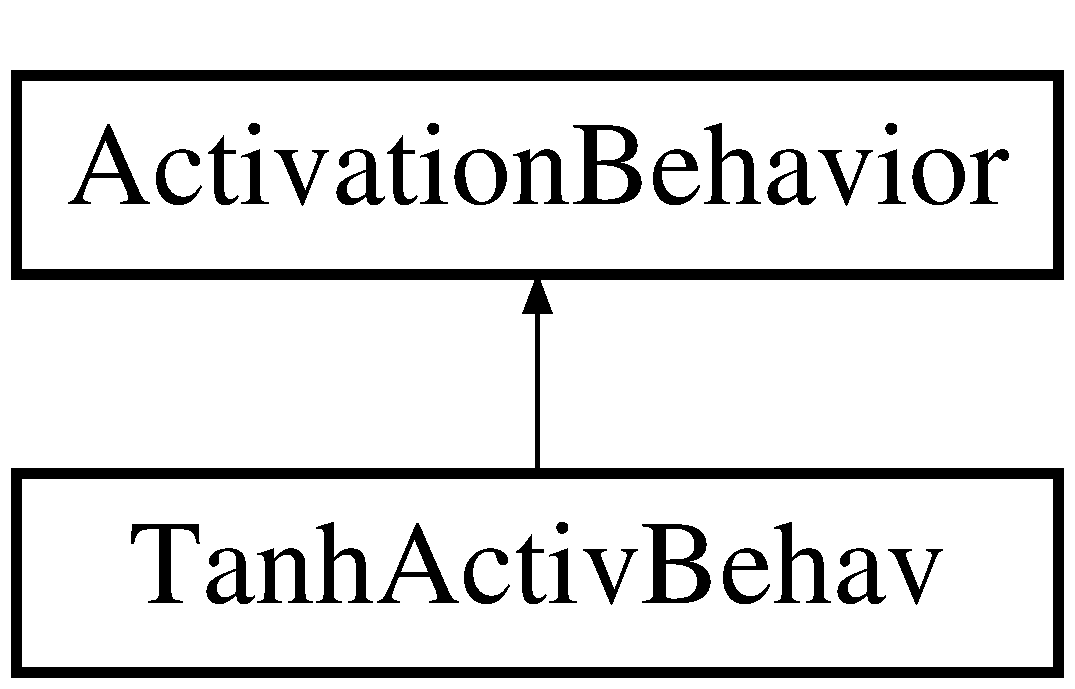
\includegraphics[height=2.000000cm]{class_tanh_activ_behav}
\end{center}
\end{figure}
\subsection*{Public Member Functions}
\begin{DoxyCompactItemize}
\item 
float \mbox{\hyperlink{class_tanh_activ_behav_a7aa47f0ab45debc7cc89d62334e28b77}{activ\+Funct}} (float input)
\end{DoxyCompactItemize}


\subsection{Detailed Description}
Implements Tanh activation function. 



\subsection{Member Function Documentation}
\mbox{\Hypertarget{class_tanh_activ_behav_a7aa47f0ab45debc7cc89d62334e28b77}\label{class_tanh_activ_behav_a7aa47f0ab45debc7cc89d62334e28b77}} 
\index{Tanh\+Activ\+Behav@{Tanh\+Activ\+Behav}!activ\+Funct@{activ\+Funct}}
\index{activ\+Funct@{activ\+Funct}!Tanh\+Activ\+Behav@{Tanh\+Activ\+Behav}}
\subsubsection{\texorpdfstring{activ\+Funct()}{activFunct()}}
{\footnotesize\ttfamily float Tanh\+Activ\+Behav.\+activ\+Funct (\begin{DoxyParamCaption}\item[{float}]{input }\end{DoxyParamCaption})}



Implements \mbox{\hyperlink{interface_activation_behavior_a6c7af51cf1b10eaadcbf086231e5539b}{Activation\+Behavior}}.



The documentation for this class was generated from the following file\+:\begin{DoxyCompactItemize}
\item 
\mbox{\hyperlink{_tanh_activ_behav_8cs}{Tanh\+Activ\+Behav.\+cs}}\end{DoxyCompactItemize}

\hypertarget{class_texture_maker_example}{}\section{Texture\+Maker\+Example Class Reference}
\label{class_texture_maker_example}\index{Texture\+Maker\+Example@{Texture\+Maker\+Example}}
Inheritance diagram for Texture\+Maker\+Example\+:\begin{figure}[H]
\begin{center}
\leavevmode
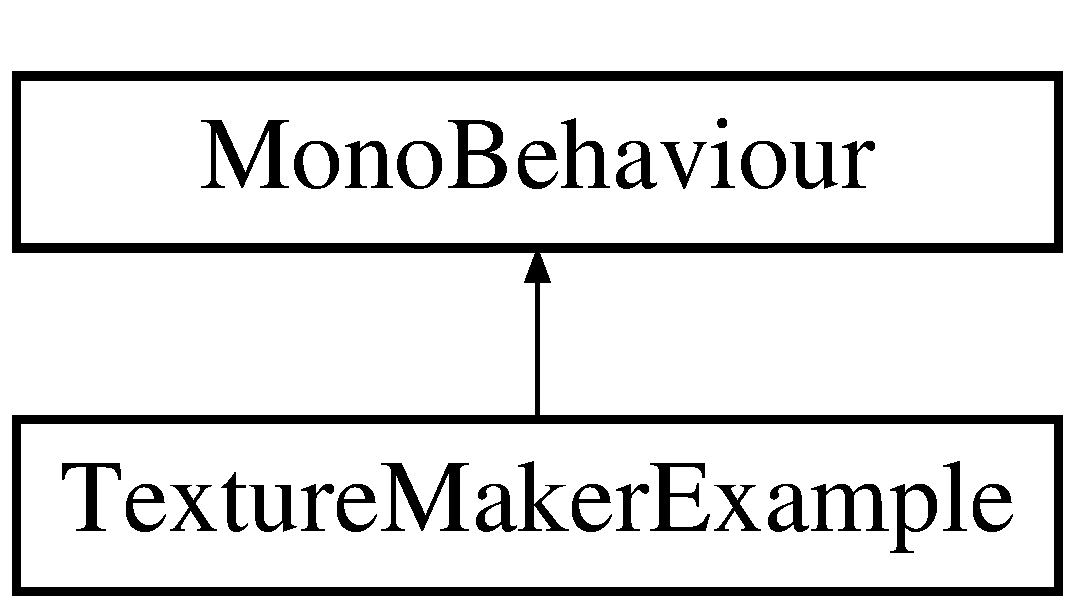
\includegraphics[height=2.000000cm]{class_texture_maker_example}
\end{center}
\end{figure}


The documentation for this class was generated from the following file\+:\begin{DoxyCompactItemize}
\item 
\mbox{\hyperlink{_texture_maker_example_8cs}{Texture\+Maker\+Example.\+cs}}\end{DoxyCompactItemize}

\hypertarget{class_thread_manager}{}\section{Thread\+Manager Class Reference}
\label{class_thread_manager}\index{Thread\+Manager@{Thread\+Manager}}
Inheritance diagram for Thread\+Manager\+:\begin{figure}[H]
\begin{center}
\leavevmode
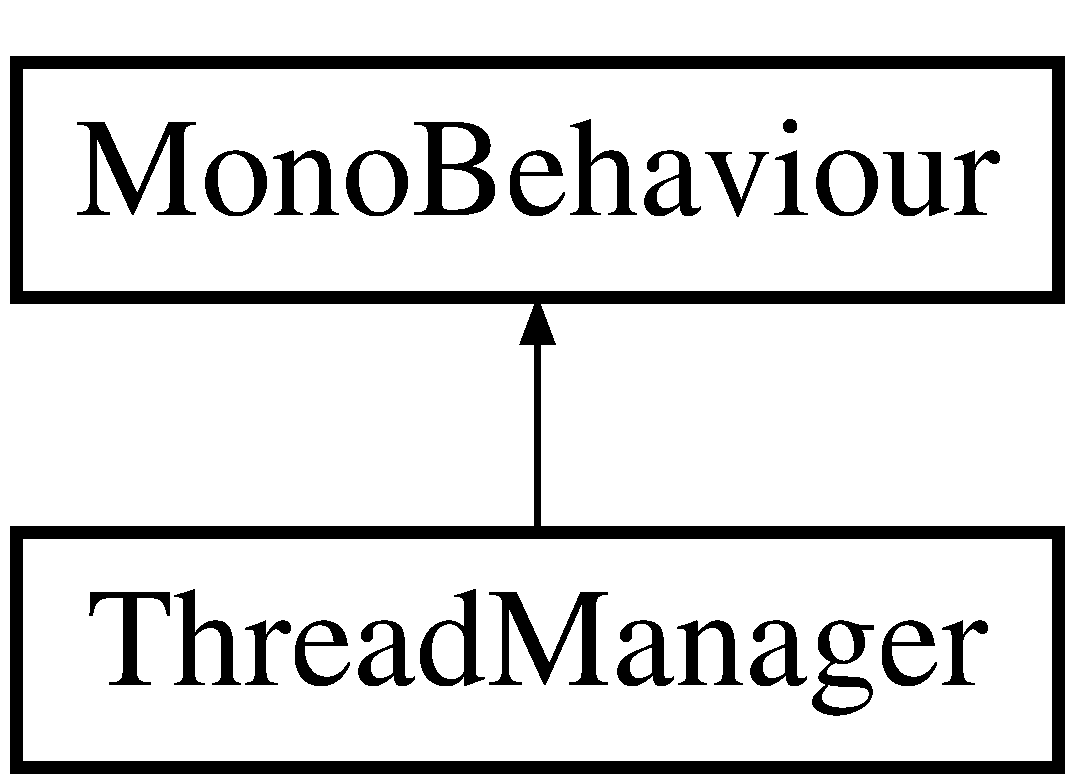
\includegraphics[height=2.000000cm]{class_thread_manager}
\end{center}
\end{figure}
\subsection*{Public Member Functions}
\begin{DoxyCompactItemize}
\item 
delegate void \mbox{\hyperlink{class_thread_manager_a31b09b282d070ea1e0d6ca52af4a64b6}{anony}} (\mbox{\hyperlink{class_ecosystem}{Ecosystem}} eco)
\item 
void \mbox{\hyperlink{class_thread_manager_a1d2756b24756d187ebf25779d623e980}{set\+Steps}} (int \+\_\+steps)
\item 
\mbox{\hyperlink{class_ecosystem}{Ecosystem}} \mbox{\hyperlink{class_thread_manager_ad8339ead9d54c051097f3b5ba3b963f3}{get\+Ecosystem}} ()
\item 
void \mbox{\hyperlink{class_thread_manager_a4dbbef51cfc289eb181c49febf97ce63}{Start\+Eco\+Sim}} ()
\item 
bool \mbox{\hyperlink{class_thread_manager_ae8fcc8db16fab19e95bf9d8dbe8be03a}{update\+Eco\+If\+Ready}} ()
\item 
void \mbox{\hyperlink{class_thread_manager_acd855802214dc3bd50bdda044fcb76ec}{Start\+Threaded\+Function}} (Thread\+Start some\+Function)
\item 
void \mbox{\hyperlink{class_thread_manager_a1924e893092403b573090341efa87380}{Queue\+Main\+Thread}} (\mbox{\hyperlink{class_ecosystem}{Ecosystem}} ecosys)
\end{DoxyCompactItemize}
\subsection*{Public Attributes}
\begin{DoxyCompactItemize}
\item 
int \mbox{\hyperlink{class_thread_manager_a2a86413c99cfa790288f86dec82ea06a}{steps}}
\end{DoxyCompactItemize}


\subsection{Member Function Documentation}
\mbox{\Hypertarget{class_thread_manager_a31b09b282d070ea1e0d6ca52af4a64b6}\label{class_thread_manager_a31b09b282d070ea1e0d6ca52af4a64b6}} 
\index{Thread\+Manager@{Thread\+Manager}!anony@{anony}}
\index{anony@{anony}!Thread\+Manager@{Thread\+Manager}}
\subsubsection{\texorpdfstring{anony()}{anony()}}
{\footnotesize\ttfamily delegate void Thread\+Manager.\+anony (\begin{DoxyParamCaption}\item[{\mbox{\hyperlink{class_ecosystem}{Ecosystem}}}]{eco }\end{DoxyParamCaption})}

\mbox{\Hypertarget{class_thread_manager_ad8339ead9d54c051097f3b5ba3b963f3}\label{class_thread_manager_ad8339ead9d54c051097f3b5ba3b963f3}} 
\index{Thread\+Manager@{Thread\+Manager}!get\+Ecosystem@{get\+Ecosystem}}
\index{get\+Ecosystem@{get\+Ecosystem}!Thread\+Manager@{Thread\+Manager}}
\subsubsection{\texorpdfstring{get\+Ecosystem()}{getEcosystem()}}
{\footnotesize\ttfamily \mbox{\hyperlink{class_ecosystem}{Ecosystem}} Thread\+Manager.\+get\+Ecosystem (\begin{DoxyParamCaption}{ }\end{DoxyParamCaption})}

\mbox{\Hypertarget{class_thread_manager_a1924e893092403b573090341efa87380}\label{class_thread_manager_a1924e893092403b573090341efa87380}} 
\index{Thread\+Manager@{Thread\+Manager}!Queue\+Main\+Thread@{Queue\+Main\+Thread}}
\index{Queue\+Main\+Thread@{Queue\+Main\+Thread}!Thread\+Manager@{Thread\+Manager}}
\subsubsection{\texorpdfstring{Queue\+Main\+Thread()}{QueueMainThread()}}
{\footnotesize\ttfamily void Thread\+Manager.\+Queue\+Main\+Thread (\begin{DoxyParamCaption}\item[{\mbox{\hyperlink{class_ecosystem}{Ecosystem}}}]{ecosys }\end{DoxyParamCaption})}

\mbox{\Hypertarget{class_thread_manager_a1d2756b24756d187ebf25779d623e980}\label{class_thread_manager_a1d2756b24756d187ebf25779d623e980}} 
\index{Thread\+Manager@{Thread\+Manager}!set\+Steps@{set\+Steps}}
\index{set\+Steps@{set\+Steps}!Thread\+Manager@{Thread\+Manager}}
\subsubsection{\texorpdfstring{set\+Steps()}{setSteps()}}
{\footnotesize\ttfamily void Thread\+Manager.\+set\+Steps (\begin{DoxyParamCaption}\item[{int}]{\+\_\+steps }\end{DoxyParamCaption})}

\mbox{\Hypertarget{class_thread_manager_a4dbbef51cfc289eb181c49febf97ce63}\label{class_thread_manager_a4dbbef51cfc289eb181c49febf97ce63}} 
\index{Thread\+Manager@{Thread\+Manager}!Start\+Eco\+Sim@{Start\+Eco\+Sim}}
\index{Start\+Eco\+Sim@{Start\+Eco\+Sim}!Thread\+Manager@{Thread\+Manager}}
\subsubsection{\texorpdfstring{Start\+Eco\+Sim()}{StartEcoSim()}}
{\footnotesize\ttfamily void Thread\+Manager.\+Start\+Eco\+Sim (\begin{DoxyParamCaption}{ }\end{DoxyParamCaption})}

\mbox{\Hypertarget{class_thread_manager_acd855802214dc3bd50bdda044fcb76ec}\label{class_thread_manager_acd855802214dc3bd50bdda044fcb76ec}} 
\index{Thread\+Manager@{Thread\+Manager}!Start\+Threaded\+Function@{Start\+Threaded\+Function}}
\index{Start\+Threaded\+Function@{Start\+Threaded\+Function}!Thread\+Manager@{Thread\+Manager}}
\subsubsection{\texorpdfstring{Start\+Threaded\+Function()}{StartThreadedFunction()}}
{\footnotesize\ttfamily void Thread\+Manager.\+Start\+Threaded\+Function (\begin{DoxyParamCaption}\item[{Thread\+Start}]{some\+Function }\end{DoxyParamCaption})}

\mbox{\Hypertarget{class_thread_manager_ae8fcc8db16fab19e95bf9d8dbe8be03a}\label{class_thread_manager_ae8fcc8db16fab19e95bf9d8dbe8be03a}} 
\index{Thread\+Manager@{Thread\+Manager}!update\+Eco\+If\+Ready@{update\+Eco\+If\+Ready}}
\index{update\+Eco\+If\+Ready@{update\+Eco\+If\+Ready}!Thread\+Manager@{Thread\+Manager}}
\subsubsection{\texorpdfstring{update\+Eco\+If\+Ready()}{updateEcoIfReady()}}
{\footnotesize\ttfamily bool Thread\+Manager.\+update\+Eco\+If\+Ready (\begin{DoxyParamCaption}{ }\end{DoxyParamCaption})}



\subsection{Member Data Documentation}
\mbox{\Hypertarget{class_thread_manager_a2a86413c99cfa790288f86dec82ea06a}\label{class_thread_manager_a2a86413c99cfa790288f86dec82ea06a}} 
\index{Thread\+Manager@{Thread\+Manager}!steps@{steps}}
\index{steps@{steps}!Thread\+Manager@{Thread\+Manager}}
\subsubsection{\texorpdfstring{steps}{steps}}
{\footnotesize\ttfamily int Thread\+Manager.\+steps}



The documentation for this class was generated from the following file\+:\begin{DoxyCompactItemize}
\item 
\mbox{\hyperlink{_thread_manager_8cs}{Thread\+Manager.\+cs}}\end{DoxyCompactItemize}

\chapter{File Documentation}
\hypertarget{_abilities_editor_8cs}{}\section{Abilities\+Editor.\+cs File Reference}
\label{_abilities_editor_8cs}\index{Abilities\+Editor.\+cs@{Abilities\+Editor.\+cs}}
\subsection*{Classes}
\begin{DoxyCompactItemize}
\item 
class \mbox{\hyperlink{class_abilities_editor}{Abilities\+Editor}}
\begin{DoxyCompactList}\small\item\em A\+PI for Abilities objects. Modifies tentative\+Abilities variable from \mbox{\hyperlink{class_creature_editor}{Creature\+Editor}} \end{DoxyCompactList}\end{DoxyCompactItemize}
\subsection*{Enumerations}
\begin{DoxyCompactItemize}
\item 
enum \mbox{\hyperlink{_abilities_editor_8cs_ae01c380f385ee9eeb03333f20711ab5a}{ability\+Type}} \{ \mbox{\hyperlink{_abilities_editor_8cs_ae01c380f385ee9eeb03333f20711ab5aa0a09521da48c718886fd7c0306a29b9e}{ability\+Type.\+comsumption}}, 
\mbox{\hyperlink{_abilities_editor_8cs_ae01c380f385ee9eeb03333f20711ab5aa39bcd1cd5b541e3782af201d5eed4c32}{ability\+Type.\+defense}}, 
\mbox{\hyperlink{_abilities_editor_8cs_ae01c380f385ee9eeb03333f20711ab5aafc7e987f23de5bd6562b7c0063cad659}{ability\+Type.\+attack}}
 \}
\end{DoxyCompactItemize}


\subsection{Enumeration Type Documentation}
\mbox{\Hypertarget{_abilities_editor_8cs_ae01c380f385ee9eeb03333f20711ab5a}\label{_abilities_editor_8cs_ae01c380f385ee9eeb03333f20711ab5a}} 
\index{Abilities\+Editor.\+cs@{Abilities\+Editor.\+cs}!ability\+Type@{ability\+Type}}
\index{ability\+Type@{ability\+Type}!Abilities\+Editor.\+cs@{Abilities\+Editor.\+cs}}
\subsubsection{\texorpdfstring{ability\+Type}{abilityType}}
{\footnotesize\ttfamily enum \mbox{\hyperlink{_abilities_editor_8cs_ae01c380f385ee9eeb03333f20711ab5a}{ability\+Type}}\hspace{0.3cm}{\ttfamily [strong]}}

\begin{DoxyEnumFields}{Enumerator}
\raisebox{\heightof{T}}[0pt][0pt]{\index{comsumption@{comsumption}!Abilities\+Editor.\+cs@{Abilities\+Editor.\+cs}}\index{Abilities\+Editor.\+cs@{Abilities\+Editor.\+cs}!comsumption@{comsumption}}}\mbox{\Hypertarget{_abilities_editor_8cs_ae01c380f385ee9eeb03333f20711ab5aa0a09521da48c718886fd7c0306a29b9e}\label{_abilities_editor_8cs_ae01c380f385ee9eeb03333f20711ab5aa0a09521da48c718886fd7c0306a29b9e}} 
comsumption&\\
\hline

\raisebox{\heightof{T}}[0pt][0pt]{\index{defense@{defense}!Abilities\+Editor.\+cs@{Abilities\+Editor.\+cs}}\index{Abilities\+Editor.\+cs@{Abilities\+Editor.\+cs}!defense@{defense}}}\mbox{\Hypertarget{_abilities_editor_8cs_ae01c380f385ee9eeb03333f20711ab5aa39bcd1cd5b541e3782af201d5eed4c32}\label{_abilities_editor_8cs_ae01c380f385ee9eeb03333f20711ab5aa39bcd1cd5b541e3782af201d5eed4c32}} 
defense&\\
\hline

\raisebox{\heightof{T}}[0pt][0pt]{\index{attack@{attack}!Abilities\+Editor.\+cs@{Abilities\+Editor.\+cs}}\index{Abilities\+Editor.\+cs@{Abilities\+Editor.\+cs}!attack@{attack}}}\mbox{\Hypertarget{_abilities_editor_8cs_ae01c380f385ee9eeb03333f20711ab5aafc7e987f23de5bd6562b7c0063cad659}\label{_abilities_editor_8cs_ae01c380f385ee9eeb03333f20711ab5aafc7e987f23de5bd6562b7c0063cad659}} 
attack&\\
\hline

\end{DoxyEnumFields}

\hypertarget{_ability_8cs}{}\section{Ability.\+cs File Reference}
\label{_ability_8cs}\index{Ability.\+cs@{Ability.\+cs}}
\subsection*{Classes}
\begin{DoxyCompactItemize}
\item 
class \mbox{\hyperlink{class_ability}{Ability}}
\begin{DoxyCompactList}\small\item\em Modifies creature\textquotesingle{}s ability to consume certain resources or attack certain species. Each creature has a specific number of ability points to assign to different abilities. \end{DoxyCompactList}\end{DoxyCompactItemize}

\hypertarget{_action_8cs}{}\section{Action.\+cs File Reference}
\label{_action_8cs}\index{Action.\+cs@{Action.\+cs}}
\subsection*{Classes}
\begin{DoxyCompactItemize}
\item 
class \mbox{\hyperlink{class_action}{Action}}
\end{DoxyCompactItemize}

\hypertarget{_action_editor_8cs}{}\section{Action\+Editor.\+cs File Reference}
\label{_action_editor_8cs}\index{Action\+Editor.\+cs@{Action\+Editor.\+cs}}
\subsection*{Classes}
\begin{DoxyCompactItemize}
\item 
class \mbox{\hyperlink{class_action_editor}{Action\+Editor}}
\end{DoxyCompactItemize}
\subsection*{Enumerations}
\begin{DoxyCompactItemize}
\item 
enum \mbox{\hyperlink{_action_editor_8cs_a1f6dfc24cb6beb094c3b5a7ad73c805a}{Action\+Creator\+Type}} \{ \mbox{\hyperlink{_action_editor_8cs_a1f6dfc24cb6beb094c3b5a7ad73c805aa996dd81c640b4ad2fdc66ab3a6888ade}{Action\+Creator\+Type.\+comm\+Action\+Creator}}, 
\mbox{\hyperlink{_action_editor_8cs_a1f6dfc24cb6beb094c3b5a7ad73c805aab4cb122edc85c8c6605458b78f3f7db4}{Action\+Creator\+Type.\+move\+Action\+Creator}}, 
\mbox{\hyperlink{_action_editor_8cs_a1f6dfc24cb6beb094c3b5a7ad73c805aa5ffdfaa05f4f10dbcdd70f50a8be915e}{Action\+Creator\+Type.\+consume\+Creator}}, 
\mbox{\hyperlink{_action_editor_8cs_a1f6dfc24cb6beb094c3b5a7ad73c805aac45bd19629b8c70d587759aa9d0a1773}{Action\+Creator\+Type.\+reproduce\+Creator}}
 \}
\end{DoxyCompactItemize}


\subsection{Enumeration Type Documentation}
\mbox{\Hypertarget{_action_editor_8cs_a1f6dfc24cb6beb094c3b5a7ad73c805a}\label{_action_editor_8cs_a1f6dfc24cb6beb094c3b5a7ad73c805a}} 
\index{Action\+Editor.\+cs@{Action\+Editor.\+cs}!Action\+Creator\+Type@{Action\+Creator\+Type}}
\index{Action\+Creator\+Type@{Action\+Creator\+Type}!Action\+Editor.\+cs@{Action\+Editor.\+cs}}
\subsubsection{\texorpdfstring{Action\+Creator\+Type}{ActionCreatorType}}
{\footnotesize\ttfamily enum \mbox{\hyperlink{_action_editor_8cs_a1f6dfc24cb6beb094c3b5a7ad73c805a}{Action\+Creator\+Type}}\hspace{0.3cm}{\ttfamily [strong]}}

\begin{DoxyEnumFields}{Enumerator}
\raisebox{\heightof{T}}[0pt][0pt]{\index{comm\+Action\+Creator@{comm\+Action\+Creator}!Action\+Editor.\+cs@{Action\+Editor.\+cs}}\index{Action\+Editor.\+cs@{Action\+Editor.\+cs}!comm\+Action\+Creator@{comm\+Action\+Creator}}}\mbox{\Hypertarget{_action_editor_8cs_a1f6dfc24cb6beb094c3b5a7ad73c805aa996dd81c640b4ad2fdc66ab3a6888ade}\label{_action_editor_8cs_a1f6dfc24cb6beb094c3b5a7ad73c805aa996dd81c640b4ad2fdc66ab3a6888ade}} 
comm\+Action\+Creator&\\
\hline

\raisebox{\heightof{T}}[0pt][0pt]{\index{move\+Action\+Creator@{move\+Action\+Creator}!Action\+Editor.\+cs@{Action\+Editor.\+cs}}\index{Action\+Editor.\+cs@{Action\+Editor.\+cs}!move\+Action\+Creator@{move\+Action\+Creator}}}\mbox{\Hypertarget{_action_editor_8cs_a1f6dfc24cb6beb094c3b5a7ad73c805aab4cb122edc85c8c6605458b78f3f7db4}\label{_action_editor_8cs_a1f6dfc24cb6beb094c3b5a7ad73c805aab4cb122edc85c8c6605458b78f3f7db4}} 
move\+Action\+Creator&\\
\hline

\raisebox{\heightof{T}}[0pt][0pt]{\index{consume\+Creator@{consume\+Creator}!Action\+Editor.\+cs@{Action\+Editor.\+cs}}\index{Action\+Editor.\+cs@{Action\+Editor.\+cs}!consume\+Creator@{consume\+Creator}}}\mbox{\Hypertarget{_action_editor_8cs_a1f6dfc24cb6beb094c3b5a7ad73c805aa5ffdfaa05f4f10dbcdd70f50a8be915e}\label{_action_editor_8cs_a1f6dfc24cb6beb094c3b5a7ad73c805aa5ffdfaa05f4f10dbcdd70f50a8be915e}} 
consume\+Creator&\\
\hline

\raisebox{\heightof{T}}[0pt][0pt]{\index{reproduce\+Creator@{reproduce\+Creator}!Action\+Editor.\+cs@{Action\+Editor.\+cs}}\index{Action\+Editor.\+cs@{Action\+Editor.\+cs}!reproduce\+Creator@{reproduce\+Creator}}}\mbox{\Hypertarget{_action_editor_8cs_a1f6dfc24cb6beb094c3b5a7ad73c805aac45bd19629b8c70d587759aa9d0a1773}\label{_action_editor_8cs_a1f6dfc24cb6beb094c3b5a7ad73c805aac45bd19629b8c70d587759aa9d0a1773}} 
reproduce\+Creator&\\
\hline

\end{DoxyEnumFields}

\hypertarget{_action_editor_abstract_8cs}{}\section{Action\+Editor\+Abstract.\+cs File Reference}
\label{_action_editor_abstract_8cs}\index{Action\+Editor\+Abstract.\+cs@{Action\+Editor\+Abstract.\+cs}}
\subsection*{Classes}
\begin{DoxyCompactItemize}
\item 
class \mbox{\hyperlink{class_action_editor_abstract}{Action\+Editor\+Abstract}}
\end{DoxyCompactItemize}

\hypertarget{_activation_behavior_8cs}{}\section{Activation\+Behavior.\+cs File Reference}
\label{_activation_behavior_8cs}\index{Activation\+Behavior.\+cs@{Activation\+Behavior.\+cs}}
\subsection*{Classes}
\begin{DoxyCompactItemize}
\item 
interface \mbox{\hyperlink{interface_activation_behavior}{Activation\+Behavior}}
\begin{DoxyCompactList}\small\item\em Interface for objects that implement an activation function. \end{DoxyCompactList}\end{DoxyCompactItemize}

\hypertarget{_bias_node_8cs}{}\section{Bias\+Node.\+cs File Reference}
\label{_bias_node_8cs}\index{Bias\+Node.\+cs@{Bias\+Node.\+cs}}
\subsection*{Classes}
\begin{DoxyCompactItemize}
\item 
class \mbox{\hyperlink{class_bias_node}{Bias\+Node}}
\end{DoxyCompactItemize}

\hypertarget{_boost_requirement_8cs}{}\section{Boost\+Requirement.\+cs File Reference}
\label{_boost_requirement_8cs}\index{Boost\+Requirement.\+cs@{Boost\+Requirement.\+cs}}
\subsection*{Classes}
\begin{DoxyCompactItemize}
\item 
class \mbox{\hyperlink{class_boost_requirement}{Boost\+Requirement}}
\begin{DoxyCompactList}\small\item\em Currently not used. Boost requirements allow for modifications to abilities, thus giving creatures with certain resources an advantage over other creatures. If all creatures are capable of this ability, and have the same boost requirements, they all have the opportunity to gain this advantage. However, it should be noted that the relationship between resources and abilities established here does give certain resources more inherent value than others. \end{DoxyCompactList}\end{DoxyCompactItemize}

\hypertarget{_camera_positioner_8cs}{}\section{Camera\+Positioner.\+cs File Reference}
\label{_camera_positioner_8cs}\index{Camera\+Positioner.\+cs@{Camera\+Positioner.\+cs}}
\subsection*{Classes}
\begin{DoxyCompactItemize}
\item 
class \mbox{\hyperlink{class_camera_positioner}{Camera\+Positioner}}
\end{DoxyCompactItemize}

\hypertarget{_comm_action_8cs}{}\section{Comm\+Action.\+cs File Reference}
\label{_comm_action_8cs}\index{Comm\+Action.\+cs@{Comm\+Action.\+cs}}
\subsection*{Classes}
\begin{DoxyCompactItemize}
\item 
class \mbox{\hyperlink{class_comm_action}{Comm\+Action}}
\end{DoxyCompactItemize}

\hypertarget{_comm_action_editor_8cs}{}\section{Comm\+Action\+Editor.\+cs File Reference}
\label{_comm_action_editor_8cs}\index{Comm\+Action\+Editor.\+cs@{Comm\+Action\+Editor.\+cs}}
\subsection*{Classes}
\begin{DoxyCompactItemize}
\item 
class \mbox{\hyperlink{class_comm_action_editor}{Comm\+Action\+Editor}}
\end{DoxyCompactItemize}

\hypertarget{_comm_input_node_8cs}{}\section{Comm\+Input\+Node.\+cs File Reference}
\label{_comm_input_node_8cs}\index{Comm\+Input\+Node.\+cs@{Comm\+Input\+Node.\+cs}}
\subsection*{Classes}
\begin{DoxyCompactItemize}
\item 
class \mbox{\hyperlink{class_comm_input_node}{Comm\+Input\+Node}}
\end{DoxyCompactItemize}

\hypertarget{_comm_network_8cs}{}\section{Comm\+Network.\+cs File Reference}
\label{_comm_network_8cs}\index{Comm\+Network.\+cs@{Comm\+Network.\+cs}}
\subsection*{Classes}
\begin{DoxyCompactItemize}
\item 
class \mbox{\hyperlink{class_comm_network}{Comm\+Network}}
\begin{DoxyCompactList}\small\item\em A network that converts incomming comm signals into action recommendations. A seperate comm network is needed for every neightbor that sends a comm signal. \end{DoxyCompactList}\end{DoxyCompactItemize}

\hypertarget{_comm_node_editor_8cs}{}\section{Comm\+Node\+Editor.\+cs File Reference}
\label{_comm_node_editor_8cs}\index{Comm\+Node\+Editor.\+cs@{Comm\+Node\+Editor.\+cs}}
\subsection*{Classes}
\begin{DoxyCompactItemize}
\item 
class \mbox{\hyperlink{class_comm_node_editor}{Comm\+Node\+Editor}}
\begin{DoxyCompactList}\small\item\em A\+PI for Comm Nodes \end{DoxyCompactList}\end{DoxyCompactItemize}

\hypertarget{_comm_signal_8cs}{}\section{Comm\+Signal.\+cs File Reference}
\label{_comm_signal_8cs}\index{Comm\+Signal.\+cs@{Comm\+Signal.\+cs}}
\subsection*{Classes}
\begin{DoxyCompactItemize}
\item 
class \mbox{\hyperlink{class_comm_signal}{Comm\+Signal}}
\begin{DoxyCompactList}\small\item\em The comm network must individually process each comm signal stored in the creatures comm\+List, and save the outputs as action recommendations. \end{DoxyCompactList}\end{DoxyCompactItemize}

\hypertarget{_consume_from_land_8cs}{}\section{Consume\+From\+Land.\+cs File Reference}
\label{_consume_from_land_8cs}\index{Consume\+From\+Land.\+cs@{Consume\+From\+Land.\+cs}}
\subsection*{Classes}
\begin{DoxyCompactItemize}
\item 
class \mbox{\hyperlink{class_consume_from_land}{Consume\+From\+Land}}
\end{DoxyCompactItemize}

\hypertarget{_consume_from_land_editor_8cs}{}\section{Consume\+From\+Land\+Editor.\+cs File Reference}
\label{_consume_from_land_editor_8cs}\index{Consume\+From\+Land\+Editor.\+cs@{Consume\+From\+Land\+Editor.\+cs}}
\subsection*{Classes}
\begin{DoxyCompactItemize}
\item 
class \mbox{\hyperlink{class_consume_from_land_editor}{Consume\+From\+Land\+Editor}}
\end{DoxyCompactItemize}

\hypertarget{_copier_8cs}{}\section{Copier.\+cs File Reference}
\label{_copier_8cs}\index{Copier.\+cs@{Copier.\+cs}}
\subsection*{Classes}
\begin{DoxyCompactItemize}
\item 
class \mbox{\hyperlink{class_copier}{Copier}}
\end{DoxyCompactItemize}

\hypertarget{_creat_menu_behav_8cs}{}\section{Creat\+Menu\+Behav.\+cs File Reference}
\label{_creat_menu_behav_8cs}\index{Creat\+Menu\+Behav.\+cs@{Creat\+Menu\+Behav.\+cs}}
\subsection*{Classes}
\begin{DoxyCompactItemize}
\item 
class \mbox{\hyperlink{class_creat_menu_behav}{Creat\+Menu\+Behav}}
\end{DoxyCompactItemize}

\hypertarget{_creature_8cs}{}\section{Creature.\+cs File Reference}
\label{_creature_8cs}\index{Creature.\+cs@{Creature.\+cs}}
\subsection*{Classes}
\begin{DoxyCompactItemize}
\item 
class \mbox{\hyperlink{class_creature}{Creature}}
\begin{DoxyCompactList}\small\item\em Class for storing all data about a creature/agent, including its neural networks, queued actions, stored resources, location and other parameters. \end{DoxyCompactList}\end{DoxyCompactItemize}

\hypertarget{_creature_editor_8cs}{}\section{Creature\+Editor.\+cs File Reference}
\label{_creature_editor_8cs}\index{Creature\+Editor.\+cs@{Creature\+Editor.\+cs}}
\subsection*{Classes}
\begin{DoxyCompactItemize}
\item 
class \mbox{\hyperlink{class_creature_editor}{Creature\+Editor}}
\end{DoxyCompactItemize}
\subsection*{Enumerations}
\begin{DoxyCompactItemize}
\item 
enum \mbox{\hyperlink{_creature_editor_8cs_a2d31a955c823bd51aec8f913e263723c}{Color\+Choice}} \{ \mbox{\hyperlink{_creature_editor_8cs_a2d31a955c823bd51aec8f913e263723cabda9643ac6601722a28f238714274da4}{Color\+Choice.\+red}}, 
\mbox{\hyperlink{_creature_editor_8cs_a2d31a955c823bd51aec8f913e263723ca9f27410725ab8cc8854a2769c7a516b8}{Color\+Choice.\+green}}, 
\mbox{\hyperlink{_creature_editor_8cs_a2d31a955c823bd51aec8f913e263723ca48d6215903dff56238e52e8891380c8f}{Color\+Choice.\+blue}}
 \}
\end{DoxyCompactItemize}


\subsection{Enumeration Type Documentation}
\mbox{\Hypertarget{_creature_editor_8cs_a2d31a955c823bd51aec8f913e263723c}\label{_creature_editor_8cs_a2d31a955c823bd51aec8f913e263723c}} 
\index{Creature\+Editor.\+cs@{Creature\+Editor.\+cs}!Color\+Choice@{Color\+Choice}}
\index{Color\+Choice@{Color\+Choice}!Creature\+Editor.\+cs@{Creature\+Editor.\+cs}}
\subsubsection{\texorpdfstring{Color\+Choice}{ColorChoice}}
{\footnotesize\ttfamily enum \mbox{\hyperlink{_creature_editor_8cs_a2d31a955c823bd51aec8f913e263723c}{Color\+Choice}}\hspace{0.3cm}{\ttfamily [strong]}}

\begin{DoxyEnumFields}{Enumerator}
\raisebox{\heightof{T}}[0pt][0pt]{\index{red@{red}!Creature\+Editor.\+cs@{Creature\+Editor.\+cs}}\index{Creature\+Editor.\+cs@{Creature\+Editor.\+cs}!red@{red}}}\mbox{\Hypertarget{_creature_editor_8cs_a2d31a955c823bd51aec8f913e263723cabda9643ac6601722a28f238714274da4}\label{_creature_editor_8cs_a2d31a955c823bd51aec8f913e263723cabda9643ac6601722a28f238714274da4}} 
red&\\
\hline

\raisebox{\heightof{T}}[0pt][0pt]{\index{green@{green}!Creature\+Editor.\+cs@{Creature\+Editor.\+cs}}\index{Creature\+Editor.\+cs@{Creature\+Editor.\+cs}!green@{green}}}\mbox{\Hypertarget{_creature_editor_8cs_a2d31a955c823bd51aec8f913e263723ca9f27410725ab8cc8854a2769c7a516b8}\label{_creature_editor_8cs_a2d31a955c823bd51aec8f913e263723ca9f27410725ab8cc8854a2769c7a516b8}} 
green&\\
\hline

\raisebox{\heightof{T}}[0pt][0pt]{\index{blue@{blue}!Creature\+Editor.\+cs@{Creature\+Editor.\+cs}}\index{Creature\+Editor.\+cs@{Creature\+Editor.\+cs}!blue@{blue}}}\mbox{\Hypertarget{_creature_editor_8cs_a2d31a955c823bd51aec8f913e263723ca48d6215903dff56238e52e8891380c8f}\label{_creature_editor_8cs_a2d31a955c823bd51aec8f913e263723ca48d6215903dff56238e52e8891380c8f}} 
blue&\\
\hline

\end{DoxyEnumFields}

\hypertarget{_creature_resource_8cs}{}\section{Creature\+Resource.\+cs File Reference}
\label{_creature_resource_8cs}\index{Creature\+Resource.\+cs@{Creature\+Resource.\+cs}}
\subsection*{Classes}
\begin{DoxyCompactItemize}
\item 
class \mbox{\hyperlink{class_creature_resource}{Creature\+Resource}}
\begin{DoxyCompactList}\small\item\em Resource stored by a creature, and how that resource effects the creature. \end{DoxyCompactList}\end{DoxyCompactItemize}

\hypertarget{_eco_manager_8cs}{}\section{Eco\+Manager.\+cs File Reference}
\label{_eco_manager_8cs}\index{Eco\+Manager.\+cs@{Eco\+Manager.\+cs}}
\subsection*{Classes}
\begin{DoxyCompactItemize}
\item 
class \mbox{\hyperlink{class_eco_manager}{Eco\+Manager}}
\end{DoxyCompactItemize}

\hypertarget{_eco_menu_behav_8cs}{}\section{Eco\+Menu\+Behav.\+cs File Reference}
\label{_eco_menu_behav_8cs}\index{Eco\+Menu\+Behav.\+cs@{Eco\+Menu\+Behav.\+cs}}
\subsection*{Classes}
\begin{DoxyCompactItemize}
\item 
class \mbox{\hyperlink{class_eco_menu_behav}{Eco\+Menu\+Behav}}
\end{DoxyCompactItemize}

\hypertarget{_eco_menu_tester_8cs}{}\section{Eco\+Menu\+Tester.\+cs File Reference}
\label{_eco_menu_tester_8cs}\index{Eco\+Menu\+Tester.\+cs@{Eco\+Menu\+Tester.\+cs}}
\subsection*{Classes}
\begin{DoxyCompactItemize}
\item 
class \mbox{\hyperlink{class_eco_menu_tester}{Eco\+Menu\+Tester}}
\end{DoxyCompactItemize}

\hypertarget{_ecosystem_8cs}{}\section{Ecosystem.\+cs File Reference}
\label{_ecosystem_8cs}\index{Ecosystem.\+cs@{Ecosystem.\+cs}}
\subsection*{Classes}
\begin{DoxyCompactItemize}
\item 
class \mbox{\hyperlink{class_ecosystem}{Ecosystem}}
\begin{DoxyCompactList}\small\item\em This class contains all of the data about the state of the ecosystem including the populations, species templates, map, resources, and other general parameters. \end{DoxyCompactList}\end{DoxyCompactItemize}

\hypertarget{_ecosystem_editor_8cs}{}\section{Ecosystem\+Editor.\+cs File Reference}
\label{_ecosystem_editor_8cs}\index{Ecosystem\+Editor.\+cs@{Ecosystem\+Editor.\+cs}}
\subsection*{Classes}
\begin{DoxyCompactItemize}
\item 
class \mbox{\hyperlink{class_ecosystem_editor}{Ecosystem\+Editor}}
\begin{DoxyCompactList}\small\item\em A\+PI for alterning ecosystem. \end{DoxyCompactList}\end{DoxyCompactItemize}

\hypertarget{_ecosystem_getter_8cs}{}\section{Ecosystem\+Getter.\+cs File Reference}
\label{_ecosystem_getter_8cs}\index{Ecosystem\+Getter.\+cs@{Ecosystem\+Getter.\+cs}}
\subsection*{Classes}
\begin{DoxyCompactItemize}
\item 
class \mbox{\hyperlink{class_ecosystem_getter}{Ecosystem\+Getter}}
\end{DoxyCompactItemize}

\hypertarget{_empty_activ_behavior_8cs}{}\section{Empty\+Activ\+Behavior.\+cs File Reference}
\label{_empty_activ_behavior_8cs}\index{Empty\+Activ\+Behavior.\+cs@{Empty\+Activ\+Behavior.\+cs}}
\subsection*{Classes}
\begin{DoxyCompactItemize}
\item 
class \mbox{\hyperlink{class_empty_activ_behavior}{Empty\+Activ\+Behavior}}
\begin{DoxyCompactList}\small\item\em No activation function (node simply uses linear combination). \end{DoxyCompactList}\end{DoxyCompactItemize}

\hypertarget{_error_manager_8cs}{}\section{Error\+Manager.\+cs File Reference}
\label{_error_manager_8cs}\index{Error\+Manager.\+cs@{Error\+Manager.\+cs}}
\subsection*{Classes}
\begin{DoxyCompactItemize}
\item 
class \mbox{\hyperlink{class_error_manager}{Error\+Manager}}
\end{DoxyCompactItemize}

\hypertarget{_game_manager_8cs}{}\section{Game\+Manager.\+cs File Reference}
\label{_game_manager_8cs}\index{Game\+Manager.\+cs@{Game\+Manager.\+cs}}
\subsection*{Classes}
\begin{DoxyCompactItemize}
\item 
class \mbox{\hyperlink{class_game_manager}{Game\+Manager}}
\end{DoxyCompactItemize}

\hypertarget{_helper_validator_8cs}{}\section{Helper\+Validator.\+cs File Reference}
\label{_helper_validator_8cs}\index{Helper\+Validator.\+cs@{Helper\+Validator.\+cs}}
\subsection*{Classes}
\begin{DoxyCompactItemize}
\item 
class \mbox{\hyperlink{class_helper_validator}{Helper\+Validator}}
\end{DoxyCompactItemize}
\subsection*{Functions}
\begin{DoxyCompactItemize}
\item 
delegate void \mbox{\hyperlink{_helper_validator_8cs_a39d82d930145ffb7e5326699e0ef7f27}{Int\+Funct}} (int x)
\item 
delegate void \mbox{\hyperlink{_helper_validator_8cs_a960dfdb4c2811fe6c539a15632075939}{String\+Funct}} (string s)
\end{DoxyCompactItemize}


\subsection{Function Documentation}
\mbox{\Hypertarget{_helper_validator_8cs_a39d82d930145ffb7e5326699e0ef7f27}\label{_helper_validator_8cs_a39d82d930145ffb7e5326699e0ef7f27}} 
\index{Helper\+Validator.\+cs@{Helper\+Validator.\+cs}!Int\+Funct@{Int\+Funct}}
\index{Int\+Funct@{Int\+Funct}!Helper\+Validator.\+cs@{Helper\+Validator.\+cs}}
\subsubsection{\texorpdfstring{Int\+Funct()}{IntFunct()}}
{\footnotesize\ttfamily delegate void Int\+Funct (\begin{DoxyParamCaption}\item[{int}]{x }\end{DoxyParamCaption})}

\mbox{\Hypertarget{_helper_validator_8cs_a960dfdb4c2811fe6c539a15632075939}\label{_helper_validator_8cs_a960dfdb4c2811fe6c539a15632075939}} 
\index{Helper\+Validator.\+cs@{Helper\+Validator.\+cs}!String\+Funct@{String\+Funct}}
\index{String\+Funct@{String\+Funct}!Helper\+Validator.\+cs@{Helper\+Validator.\+cs}}
\subsubsection{\texorpdfstring{String\+Funct()}{StringFunct()}}
{\footnotesize\ttfamily delegate void String\+Funct (\begin{DoxyParamCaption}\item[{string}]{s }\end{DoxyParamCaption})}


\hypertarget{_i_ecosystem_editor_8cs}{}\section{I\+Ecosystem\+Editor.\+cs File Reference}
\label{_i_ecosystem_editor_8cs}\index{I\+Ecosystem\+Editor.\+cs@{I\+Ecosystem\+Editor.\+cs}}
\subsection*{Classes}
\begin{DoxyCompactItemize}
\item 
interface \mbox{\hyperlink{interface_i_ecosystem_editor}{I\+Ecosystem\+Editor}}
\end{DoxyCompactItemize}

\hypertarget{_inner_input_node_8cs}{}\section{Inner\+Input\+Node.\+cs File Reference}
\label{_inner_input_node_8cs}\index{Inner\+Input\+Node.\+cs@{Inner\+Input\+Node.\+cs}}
\subsection*{Classes}
\begin{DoxyCompactItemize}
\item 
class \mbox{\hyperlink{class_inner_input_node}{Inner\+Input\+Node}}
\end{DoxyCompactItemize}

\hypertarget{_inner_input_node_editor_8cs}{}\section{Inner\+Input\+Node\+Editor.\+cs File Reference}
\label{_inner_input_node_editor_8cs}\index{Inner\+Input\+Node\+Editor.\+cs@{Inner\+Input\+Node\+Editor.\+cs}}
\subsection*{Classes}
\begin{DoxyCompactItemize}
\item 
class \mbox{\hyperlink{class_inner_input_node_editor}{Inner\+Input\+Node\+Editor}}
\begin{DoxyCompactList}\small\item\em A\+PI for Inner\+Input\+Nodes. \end{DoxyCompactList}\end{DoxyCompactItemize}

\hypertarget{_land_8cs}{}\section{Land.\+cs File Reference}
\label{_land_8cs}\index{Land.\+cs@{Land.\+cs}}
\subsection*{Classes}
\begin{DoxyCompactItemize}
\item 
class \mbox{\hyperlink{class_land}{Land}}
\begin{DoxyCompactList}\small\item\em Class for storing data about a location on the map. Also facilitates creature\textquotesingle{}s interaction with the environment. \end{DoxyCompactList}\end{DoxyCompactItemize}

\hypertarget{_land_resource_editor_8cs}{}\section{Land\+Resource\+Editor.\+cs File Reference}
\label{_land_resource_editor_8cs}\index{Land\+Resource\+Editor.\+cs@{Land\+Resource\+Editor.\+cs}}
\subsection*{Classes}
\begin{DoxyCompactItemize}
\item 
class \mbox{\hyperlink{class_land_resource_editor}{Land\+Resource\+Editor}}
\begin{DoxyCompactList}\small\item\em Used as interface for generating \mbox{\hyperlink{class_resource_store}{Resource\+Store}} objects. \end{DoxyCompactList}\end{DoxyCompactItemize}

\hypertarget{_logistic_activ_behavior_8cs}{}\section{Logistic\+Activ\+Behavior.\+cs File Reference}
\label{_logistic_activ_behavior_8cs}\index{Logistic\+Activ\+Behavior.\+cs@{Logistic\+Activ\+Behavior.\+cs}}
\subsection*{Classes}
\begin{DoxyCompactItemize}
\item 
class \mbox{\hyperlink{class_logistic_activ_behavior}{Logistic\+Activ\+Behavior}}
\begin{DoxyCompactList}\small\item\em Implements logistic activation function. \end{DoxyCompactList}\end{DoxyCompactItemize}

\hypertarget{_logistic_with_neg_activ_behav_8cs}{}\section{Logistic\+With\+Neg\+Activ\+Behav.\+cs File Reference}
\label{_logistic_with_neg_activ_behav_8cs}\index{Logistic\+With\+Neg\+Activ\+Behav.\+cs@{Logistic\+With\+Neg\+Activ\+Behav.\+cs}}
\subsection*{Classes}
\begin{DoxyCompactItemize}
\item 
class \mbox{\hyperlink{class_logistic_with_neg_activ_behav}{Logistic\+With\+Neg\+Activ\+Behav}}
\begin{DoxyCompactList}\small\item\em Logistic activation function, but mapped to \mbox{[}-\/1,1\mbox{]} \end{DoxyCompactList}\end{DoxyCompactItemize}

\hypertarget{_l_r_menu_behav_8cs}{}\section{L\+R\+Menu\+Behav.\+cs File Reference}
\label{_l_r_menu_behav_8cs}\index{L\+R\+Menu\+Behav.\+cs@{L\+R\+Menu\+Behav.\+cs}}
\subsection*{Classes}
\begin{DoxyCompactItemize}
\item 
class \mbox{\hyperlink{class_l_r_menu_behav}{L\+R\+Menu\+Behav}}
\end{DoxyCompactItemize}

\hypertarget{_main_menu_behav_8cs}{}\section{Main\+Menu\+Behav.\+cs File Reference}
\label{_main_menu_behav_8cs}\index{Main\+Menu\+Behav.\+cs@{Main\+Menu\+Behav.\+cs}}
\subsection*{Classes}
\begin{DoxyCompactItemize}
\item 
class \mbox{\hyperlink{class_main_menu_behav}{Main\+Menu\+Behav}}
\end{DoxyCompactItemize}

\hypertarget{_map_editor_8cs}{}\section{Map\+Editor.\+cs File Reference}
\label{_map_editor_8cs}\index{Map\+Editor.\+cs@{Map\+Editor.\+cs}}
\subsection*{Classes}
\begin{DoxyCompactItemize}
\item 
class \mbox{\hyperlink{class_map_editor}{Map\+Editor}}
\begin{DoxyCompactList}\small\item\em A\+PI for editing the map\+: a 2D array of \mbox{\hyperlink{class_land}{Land}} spaces. Used to generate the map, and add resources. \end{DoxyCompactList}\end{DoxyCompactItemize}

\hypertarget{_memory_input_node_8cs}{}\section{Memory\+Input\+Node.\+cs File Reference}
\label{_memory_input_node_8cs}\index{Memory\+Input\+Node.\+cs@{Memory\+Input\+Node.\+cs}}
\subsection*{Classes}
\begin{DoxyCompactItemize}
\item 
class \mbox{\hyperlink{class_memory_input_node}{Memory\+Input\+Node}}
\end{DoxyCompactItemize}

\hypertarget{_move_action_8cs}{}\section{Move\+Action.\+cs File Reference}
\label{_move_action_8cs}\index{Move\+Action.\+cs@{Move\+Action.\+cs}}
\subsection*{Classes}
\begin{DoxyCompactItemize}
\item 
class \mbox{\hyperlink{class_move_action}{Move\+Action}}
\end{DoxyCompactItemize}
\subsection*{Enumerations}
\begin{DoxyCompactItemize}
\item 
enum \mbox{\hyperlink{_move_action_8cs_a9e4683fdca765fb08e2d0e5f7f57c162}{move\+Dir}} \{ \mbox{\hyperlink{_move_action_8cs_a9e4683fdca765fb08e2d0e5f7f57c162a46c48bec0d282018b9d167eef7711b2c}{move\+Dir.\+up}}, 
\mbox{\hyperlink{_move_action_8cs_a9e4683fdca765fb08e2d0e5f7f57c162a74e8333ad11685ff3bdae589c8f6e34d}{move\+Dir.\+down}}, 
\mbox{\hyperlink{_move_action_8cs_a9e4683fdca765fb08e2d0e5f7f57c162a811882fecd5c7618d7099ebbd39ea254}{move\+Dir.\+left}}, 
\mbox{\hyperlink{_move_action_8cs_a9e4683fdca765fb08e2d0e5f7f57c162a7c4f29407893c334a6cb7a87bf045c0d}{move\+Dir.\+right}}
 \}
\end{DoxyCompactItemize}


\subsection{Enumeration Type Documentation}
\mbox{\Hypertarget{_move_action_8cs_a9e4683fdca765fb08e2d0e5f7f57c162}\label{_move_action_8cs_a9e4683fdca765fb08e2d0e5f7f57c162}} 
\index{Move\+Action.\+cs@{Move\+Action.\+cs}!move\+Dir@{move\+Dir}}
\index{move\+Dir@{move\+Dir}!Move\+Action.\+cs@{Move\+Action.\+cs}}
\subsubsection{\texorpdfstring{move\+Dir}{moveDir}}
{\footnotesize\ttfamily enum \mbox{\hyperlink{_move_action_8cs_a9e4683fdca765fb08e2d0e5f7f57c162}{move\+Dir}}\hspace{0.3cm}{\ttfamily [strong]}}

\begin{DoxyEnumFields}{Enumerator}
\raisebox{\heightof{T}}[0pt][0pt]{\index{up@{up}!Move\+Action.\+cs@{Move\+Action.\+cs}}\index{Move\+Action.\+cs@{Move\+Action.\+cs}!up@{up}}}\mbox{\Hypertarget{_move_action_8cs_a9e4683fdca765fb08e2d0e5f7f57c162a46c48bec0d282018b9d167eef7711b2c}\label{_move_action_8cs_a9e4683fdca765fb08e2d0e5f7f57c162a46c48bec0d282018b9d167eef7711b2c}} 
up&\\
\hline

\raisebox{\heightof{T}}[0pt][0pt]{\index{down@{down}!Move\+Action.\+cs@{Move\+Action.\+cs}}\index{Move\+Action.\+cs@{Move\+Action.\+cs}!down@{down}}}\mbox{\Hypertarget{_move_action_8cs_a9e4683fdca765fb08e2d0e5f7f57c162a74e8333ad11685ff3bdae589c8f6e34d}\label{_move_action_8cs_a9e4683fdca765fb08e2d0e5f7f57c162a74e8333ad11685ff3bdae589c8f6e34d}} 
down&\\
\hline

\raisebox{\heightof{T}}[0pt][0pt]{\index{left@{left}!Move\+Action.\+cs@{Move\+Action.\+cs}}\index{Move\+Action.\+cs@{Move\+Action.\+cs}!left@{left}}}\mbox{\Hypertarget{_move_action_8cs_a9e4683fdca765fb08e2d0e5f7f57c162a811882fecd5c7618d7099ebbd39ea254}\label{_move_action_8cs_a9e4683fdca765fb08e2d0e5f7f57c162a811882fecd5c7618d7099ebbd39ea254}} 
left&\\
\hline

\raisebox{\heightof{T}}[0pt][0pt]{\index{right@{right}!Move\+Action.\+cs@{Move\+Action.\+cs}}\index{Move\+Action.\+cs@{Move\+Action.\+cs}!right@{right}}}\mbox{\Hypertarget{_move_action_8cs_a9e4683fdca765fb08e2d0e5f7f57c162a7c4f29407893c334a6cb7a87bf045c0d}\label{_move_action_8cs_a9e4683fdca765fb08e2d0e5f7f57c162a7c4f29407893c334a6cb7a87bf045c0d}} 
right&\\
\hline

\end{DoxyEnumFields}

\hypertarget{_move_action_editor_8cs}{}\section{Move\+Action\+Editor.\+cs File Reference}
\label{_move_action_editor_8cs}\index{Move\+Action\+Editor.\+cs@{Move\+Action\+Editor.\+cs}}
\subsection*{Classes}
\begin{DoxyCompactItemize}
\item 
class \mbox{\hyperlink{class_move_action_editor}{Move\+Action\+Editor}}
\end{DoxyCompactItemize}

\hypertarget{_network_8cs}{}\section{Network.\+cs File Reference}
\label{_network_8cs}\index{Network.\+cs@{Network.\+cs}}
\subsection*{Classes}
\begin{DoxyCompactItemize}
\item 
class \mbox{\hyperlink{class_network}{Network}}
\begin{DoxyCompactList}\small\item\em A neural network of a creature, which consists of layers of nodes. \end{DoxyCompactList}\end{DoxyCompactItemize}

\hypertarget{_network_editor_8cs}{}\section{Network\+Editor.\+cs File Reference}
\label{_network_editor_8cs}\index{Network\+Editor.\+cs@{Network\+Editor.\+cs}}
\subsection*{Classes}
\begin{DoxyCompactItemize}
\item 
class \mbox{\hyperlink{class_network_editor}{Network\+Editor}}
\begin{DoxyCompactList}\small\item\em A\+PI for \mbox{\hyperlink{class_network}{Network}} objects. Stored by Ecosystem\+Creator. \end{DoxyCompactList}\end{DoxyCompactItemize}

\hypertarget{_node_8cs}{}\section{Node.\+cs File Reference}
\label{_node_8cs}\index{Node.\+cs@{Node.\+cs}}
\subsection*{Classes}
\begin{DoxyCompactItemize}
\item 
class \mbox{\hyperlink{class_node}{Node}}
\begin{DoxyCompactList}\small\item\em Abstract parent class for all \mbox{\hyperlink{class_node}{Node}} types. A \mbox{\hyperlink{class_node}{Node}} represents a node in a creatures neural network. \end{DoxyCompactList}\end{DoxyCompactItemize}

\hypertarget{_node_editor_8cs}{}\section{Node\+Editor.\+cs File Reference}
\label{_node_editor_8cs}\index{Node\+Editor.\+cs@{Node\+Editor.\+cs}}
\subsection*{Classes}
\begin{DoxyCompactItemize}
\item 
class \mbox{\hyperlink{class_node_editor}{Node\+Editor}}
\begin{DoxyCompactList}\small\item\em A\+PI for storing different kinds of specific node creators. ex. -\/ could wrap a Sensory\+Input\+Node\+Creator. Stored by Network\+Creator. \end{DoxyCompactList}\end{DoxyCompactItemize}
\subsection*{Enumerations}
\begin{DoxyCompactItemize}
\item 
enum \mbox{\hyperlink{_node_editor_8cs_afc5d9fc086bcd57827af91c5d369b625}{Node\+Creator\+Type}} \{ \mbox{\hyperlink{_node_editor_8cs_afc5d9fc086bcd57827af91c5d369b625abc64d24cbb5539e9a6fb5b4a013e6f4e}{Node\+Creator\+Type.\+si\+Node\+Creator}}, 
\mbox{\hyperlink{_node_editor_8cs_afc5d9fc086bcd57827af91c5d369b625a2054fead2bbea718da9179c2c5e89a1e}{Node\+Creator\+Type.\+comm\+Node\+Creator}}, 
\mbox{\hyperlink{_node_editor_8cs_afc5d9fc086bcd57827af91c5d369b625a5c39e03c42e6bca54b86a6192fe26061}{Node\+Creator\+Type.\+output\+Node\+Creator}}, 
\mbox{\hyperlink{_node_editor_8cs_afc5d9fc086bcd57827af91c5d369b625aba13ccc7117e26518043cf644055f65d}{Node\+Creator\+Type.\+inner\+Input\+Node\+Creator}}
 \}
\end{DoxyCompactItemize}


\subsection{Enumeration Type Documentation}
\mbox{\Hypertarget{_node_editor_8cs_afc5d9fc086bcd57827af91c5d369b625}\label{_node_editor_8cs_afc5d9fc086bcd57827af91c5d369b625}} 
\index{Node\+Editor.\+cs@{Node\+Editor.\+cs}!Node\+Creator\+Type@{Node\+Creator\+Type}}
\index{Node\+Creator\+Type@{Node\+Creator\+Type}!Node\+Editor.\+cs@{Node\+Editor.\+cs}}
\subsubsection{\texorpdfstring{Node\+Creator\+Type}{NodeCreatorType}}
{\footnotesize\ttfamily enum \mbox{\hyperlink{_node_editor_8cs_afc5d9fc086bcd57827af91c5d369b625}{Node\+Creator\+Type}}\hspace{0.3cm}{\ttfamily [strong]}}

\begin{DoxyEnumFields}{Enumerator}
\raisebox{\heightof{T}}[0pt][0pt]{\index{si\+Node\+Creator@{si\+Node\+Creator}!Node\+Editor.\+cs@{Node\+Editor.\+cs}}\index{Node\+Editor.\+cs@{Node\+Editor.\+cs}!si\+Node\+Creator@{si\+Node\+Creator}}}\mbox{\Hypertarget{_node_editor_8cs_afc5d9fc086bcd57827af91c5d369b625abc64d24cbb5539e9a6fb5b4a013e6f4e}\label{_node_editor_8cs_afc5d9fc086bcd57827af91c5d369b625abc64d24cbb5539e9a6fb5b4a013e6f4e}} 
si\+Node\+Creator&\\
\hline

\raisebox{\heightof{T}}[0pt][0pt]{\index{comm\+Node\+Creator@{comm\+Node\+Creator}!Node\+Editor.\+cs@{Node\+Editor.\+cs}}\index{Node\+Editor.\+cs@{Node\+Editor.\+cs}!comm\+Node\+Creator@{comm\+Node\+Creator}}}\mbox{\Hypertarget{_node_editor_8cs_afc5d9fc086bcd57827af91c5d369b625a2054fead2bbea718da9179c2c5e89a1e}\label{_node_editor_8cs_afc5d9fc086bcd57827af91c5d369b625a2054fead2bbea718da9179c2c5e89a1e}} 
comm\+Node\+Creator&\\
\hline

\raisebox{\heightof{T}}[0pt][0pt]{\index{output\+Node\+Creator@{output\+Node\+Creator}!Node\+Editor.\+cs@{Node\+Editor.\+cs}}\index{Node\+Editor.\+cs@{Node\+Editor.\+cs}!output\+Node\+Creator@{output\+Node\+Creator}}}\mbox{\Hypertarget{_node_editor_8cs_afc5d9fc086bcd57827af91c5d369b625a5c39e03c42e6bca54b86a6192fe26061}\label{_node_editor_8cs_afc5d9fc086bcd57827af91c5d369b625a5c39e03c42e6bca54b86a6192fe26061}} 
output\+Node\+Creator&\\
\hline

\raisebox{\heightof{T}}[0pt][0pt]{\index{inner\+Input\+Node\+Creator@{inner\+Input\+Node\+Creator}!Node\+Editor.\+cs@{Node\+Editor.\+cs}}\index{Node\+Editor.\+cs@{Node\+Editor.\+cs}!inner\+Input\+Node\+Creator@{inner\+Input\+Node\+Creator}}}\mbox{\Hypertarget{_node_editor_8cs_afc5d9fc086bcd57827af91c5d369b625aba13ccc7117e26518043cf644055f65d}\label{_node_editor_8cs_afc5d9fc086bcd57827af91c5d369b625aba13ccc7117e26518043cf644055f65d}} 
inner\+Input\+Node\+Creator&\\
\hline

\end{DoxyEnumFields}

\hypertarget{_node_editor_interface_8cs}{}\section{Node\+Editor\+Interface.\+cs File Reference}
\label{_node_editor_interface_8cs}\index{Node\+Editor\+Interface.\+cs@{Node\+Editor\+Interface.\+cs}}
\subsection*{Classes}
\begin{DoxyCompactItemize}
\item 
interface \mbox{\hyperlink{interface_node_editor_interface}{Node\+Editor\+Interface}}
\begin{DoxyCompactList}\small\item\em Interface that allows all specific node creator objects to be stored by Node\+Creator class. \end{DoxyCompactList}\end{DoxyCompactItemize}

\hypertarget{_non_input_node_8cs}{}\section{Non\+Input\+Node.\+cs File Reference}
\label{_non_input_node_8cs}\index{Non\+Input\+Node.\+cs@{Non\+Input\+Node.\+cs}}
\subsection*{Classes}
\begin{DoxyCompactItemize}
\item 
class \mbox{\hyperlink{class_non_input_node}{Non\+Input\+Node}}
\begin{DoxyCompactList}\small\item\em Encompasses hidden nodes (which use this class directly) and output nodes (which use the \mbox{\hyperlink{class_output_node}{Output\+Node}} class). \end{DoxyCompactList}\end{DoxyCompactItemize}
\subsection*{Enumerations}
\begin{DoxyCompactItemize}
\item 
enum \mbox{\hyperlink{_non_input_node_8cs_a832a6943e91e304dea9608c4ae2818e7}{Activation\+Behavior\+Types}} \{ \mbox{\hyperlink{_non_input_node_8cs_a832a6943e91e304dea9608c4ae2818e7a6cca73b743bdd7fe89b93540cd868dff}{Activation\+Behavior\+Types.\+Logistic\+AB}}, 
\mbox{\hyperlink{_non_input_node_8cs_a832a6943e91e304dea9608c4ae2818e7a1396c2292c208ac1da12219cf207d133}{Activation\+Behavior\+Types.\+Empty\+AB}}, 
\mbox{\hyperlink{_non_input_node_8cs_a832a6943e91e304dea9608c4ae2818e7af2402b1df9cebc5c237f903cd9b3087b}{Activation\+Behavior\+Types.\+Log\+With\+Neg}}, 
\mbox{\hyperlink{_non_input_node_8cs_a832a6943e91e304dea9608c4ae2818e7acc132a41cab5676334f353a22a0aa5c5}{Activation\+Behavior\+Types.\+Tanh}}
 \}
\end{DoxyCompactItemize}


\subsection{Enumeration Type Documentation}
\mbox{\Hypertarget{_non_input_node_8cs_a832a6943e91e304dea9608c4ae2818e7}\label{_non_input_node_8cs_a832a6943e91e304dea9608c4ae2818e7}} 
\index{Non\+Input\+Node.\+cs@{Non\+Input\+Node.\+cs}!Activation\+Behavior\+Types@{Activation\+Behavior\+Types}}
\index{Activation\+Behavior\+Types@{Activation\+Behavior\+Types}!Non\+Input\+Node.\+cs@{Non\+Input\+Node.\+cs}}
\subsubsection{\texorpdfstring{Activation\+Behavior\+Types}{ActivationBehaviorTypes}}
{\footnotesize\ttfamily enum \mbox{\hyperlink{_non_input_node_8cs_a832a6943e91e304dea9608c4ae2818e7}{Activation\+Behavior\+Types}}\hspace{0.3cm}{\ttfamily [strong]}}

\begin{DoxyEnumFields}{Enumerator}
\raisebox{\heightof{T}}[0pt][0pt]{\index{Logistic\+AB@{Logistic\+AB}!Non\+Input\+Node.\+cs@{Non\+Input\+Node.\+cs}}\index{Non\+Input\+Node.\+cs@{Non\+Input\+Node.\+cs}!Logistic\+AB@{Logistic\+AB}}}\mbox{\Hypertarget{_non_input_node_8cs_a832a6943e91e304dea9608c4ae2818e7a6cca73b743bdd7fe89b93540cd868dff}\label{_non_input_node_8cs_a832a6943e91e304dea9608c4ae2818e7a6cca73b743bdd7fe89b93540cd868dff}} 
Logistic\+AB&\\
\hline

\raisebox{\heightof{T}}[0pt][0pt]{\index{Empty\+AB@{Empty\+AB}!Non\+Input\+Node.\+cs@{Non\+Input\+Node.\+cs}}\index{Non\+Input\+Node.\+cs@{Non\+Input\+Node.\+cs}!Empty\+AB@{Empty\+AB}}}\mbox{\Hypertarget{_non_input_node_8cs_a832a6943e91e304dea9608c4ae2818e7a1396c2292c208ac1da12219cf207d133}\label{_non_input_node_8cs_a832a6943e91e304dea9608c4ae2818e7a1396c2292c208ac1da12219cf207d133}} 
Empty\+AB&\\
\hline

\raisebox{\heightof{T}}[0pt][0pt]{\index{Log\+With\+Neg@{Log\+With\+Neg}!Non\+Input\+Node.\+cs@{Non\+Input\+Node.\+cs}}\index{Non\+Input\+Node.\+cs@{Non\+Input\+Node.\+cs}!Log\+With\+Neg@{Log\+With\+Neg}}}\mbox{\Hypertarget{_non_input_node_8cs_a832a6943e91e304dea9608c4ae2818e7af2402b1df9cebc5c237f903cd9b3087b}\label{_non_input_node_8cs_a832a6943e91e304dea9608c4ae2818e7af2402b1df9cebc5c237f903cd9b3087b}} 
Log\+With\+Neg&\\
\hline

\raisebox{\heightof{T}}[0pt][0pt]{\index{Tanh@{Tanh}!Non\+Input\+Node.\+cs@{Non\+Input\+Node.\+cs}}\index{Non\+Input\+Node.\+cs@{Non\+Input\+Node.\+cs}!Tanh@{Tanh}}}\mbox{\Hypertarget{_non_input_node_8cs_a832a6943e91e304dea9608c4ae2818e7acc132a41cab5676334f353a22a0aa5c5}\label{_non_input_node_8cs_a832a6943e91e304dea9608c4ae2818e7acc132a41cab5676334f353a22a0aa5c5}} 
Tanh&\\
\hline

\end{DoxyEnumFields}

\hypertarget{_output_node_8cs}{}\section{Output\+Node.\+cs File Reference}
\label{_output_node_8cs}\index{Output\+Node.\+cs@{Output\+Node.\+cs}}
\subsection*{Classes}
\begin{DoxyCompactItemize}
\item 
class \mbox{\hyperlink{class_output_node}{Output\+Node}}
\begin{DoxyCompactList}\small\item\em Maps a the value of the node (as calculated by \mbox{\hyperlink{class_non_input_node}{Non\+Input\+Node}} methods) to an action. \end{DoxyCompactList}\end{DoxyCompactItemize}

\hypertarget{_output_node_editor_8cs}{}\section{Output\+Node\+Editor.\+cs File Reference}
\label{_output_node_editor_8cs}\index{Output\+Node\+Editor.\+cs@{Output\+Node\+Editor.\+cs}}
\subsection*{Classes}
\begin{DoxyCompactItemize}
\item 
class \mbox{\hyperlink{class_output_node_editor}{Output\+Node\+Editor}}
\begin{DoxyCompactList}\small\item\em A\+PI for Output\+Nodes. \end{DoxyCompactList}\end{DoxyCompactItemize}

\hypertarget{_population_8cs}{}\section{Population.\+cs File Reference}
\label{_population_8cs}\index{Population.\+cs@{Population.\+cs}}
\subsection*{Classes}
\begin{DoxyCompactItemize}
\item 
class \mbox{\hyperlink{class_population}{Population}}
\begin{DoxyCompactList}\small\item\em A population stores information about a list of creatures, including it\textquotesingle{}s founder, and initial variation. \end{DoxyCompactList}\end{DoxyCompactItemize}

\hypertarget{_repro_action_8cs}{}\section{Repro\+Action.\+cs File Reference}
\label{_repro_action_8cs}\index{Repro\+Action.\+cs@{Repro\+Action.\+cs}}
\subsection*{Classes}
\begin{DoxyCompactItemize}
\item 
class \mbox{\hyperlink{class_repro_action}{Repro\+Action}}
\end{DoxyCompactItemize}

\hypertarget{_repro_action_editor_8cs}{}\section{Repro\+Action\+Editor.\+cs File Reference}
\label{_repro_action_editor_8cs}\index{Repro\+Action\+Editor.\+cs@{Repro\+Action\+Editor.\+cs}}
\subsection*{Classes}
\begin{DoxyCompactItemize}
\item 
class \mbox{\hyperlink{class_repro_action_editor}{Repro\+Action\+Editor}}
\end{DoxyCompactItemize}

\hypertarget{_repro_network_8cs}{}\section{Repro\+Network.\+cs File Reference}
\label{_repro_network_8cs}\index{Repro\+Network.\+cs@{Repro\+Network.\+cs}}
\subsection*{Classes}
\begin{DoxyCompactItemize}
\item 
class \mbox{\hyperlink{class_repro_network}{Repro\+Network}}
\begin{DoxyCompactList}\small\item\em A specific kind of network that decided whether a creature should reproduce. \end{DoxyCompactList}\end{DoxyCompactItemize}

\hypertarget{_resource_editor_8cs}{}\section{Resource\+Editor.\+cs File Reference}
\label{_resource_editor_8cs}\index{Resource\+Editor.\+cs@{Resource\+Editor.\+cs}}
\subsection*{Classes}
\begin{DoxyCompactItemize}
\item 
class \mbox{\hyperlink{class_resource_editor}{Resource\+Editor}}
\begin{DoxyCompactList}\small\item\em A\+PI for setting resources that creature can store, and how the resource effects the creature. \end{DoxyCompactList}\end{DoxyCompactItemize}

\hypertarget{_resource_store_8cs}{}\section{Resource\+Store.\+cs File Reference}
\label{_resource_store_8cs}\index{Resource\+Store.\+cs@{Resource\+Store.\+cs}}
\subsection*{Classes}
\begin{DoxyCompactItemize}
\item 
class \mbox{\hyperlink{class_resource_store}{Resource\+Store}}
\begin{DoxyCompactList}\small\item\em Basic unit of a resource to be stored in a \mbox{\hyperlink{class_land}{Land}} object. \mbox{\hyperlink{class_creature}{Creature}} can attempt to consume this resource from the land. \end{DoxyCompactList}\end{DoxyCompactItemize}

\hypertarget{_sensory_input_node_8cs}{}\section{Sensory\+Input\+Node.\+cs File Reference}
\label{_sensory_input_node_8cs}\index{Sensory\+Input\+Node.\+cs@{Sensory\+Input\+Node.\+cs}}
\subsection*{Classes}
\begin{DoxyCompactItemize}
\item 
class \mbox{\hyperlink{class_sensory_input_node}{Sensory\+Input\+Node}}
\end{DoxyCompactItemize}

\hypertarget{_sensory_input_node_editor_8cs}{}\section{Sensory\+Input\+Node\+Editor.\+cs File Reference}
\label{_sensory_input_node_editor_8cs}\index{Sensory\+Input\+Node\+Editor.\+cs@{Sensory\+Input\+Node\+Editor.\+cs}}
\subsection*{Classes}
\begin{DoxyCompactItemize}
\item 
class \mbox{\hyperlink{class_sensory_input_node_editor}{Sensory\+Input\+Node\+Editor}}
\begin{DoxyCompactList}\small\item\em A\+PI for Sensory\+Input\+Nodes. \end{DoxyCompactList}\end{DoxyCompactItemize}

\hypertarget{_sim_runner_test_8cs}{}\section{Sim\+Runner\+Test.\+cs File Reference}
\label{_sim_runner_test_8cs}\index{Sim\+Runner\+Test.\+cs@{Sim\+Runner\+Test.\+cs}}
\subsection*{Classes}
\begin{DoxyCompactItemize}
\item 
class \mbox{\hyperlink{class_sim_runner_test}{Sim\+Runner\+Test}}
\begin{DoxyCompactList}\small\item\em Class for running simulation. \end{DoxyCompactList}\end{DoxyCompactItemize}

\hypertarget{_sim_runner_user_8cs}{}\section{Sim\+Runner\+User.\+cs File Reference}
\label{_sim_runner_user_8cs}\index{Sim\+Runner\+User.\+cs@{Sim\+Runner\+User.\+cs}}
\subsection*{Classes}
\begin{DoxyCompactItemize}
\item 
class \mbox{\hyperlink{class_sim_runner_user}{Sim\+Runner\+User}}
\begin{DoxyCompactList}\small\item\em Class for running simulation. \end{DoxyCompactList}\end{DoxyCompactItemize}

\hypertarget{_species_populator_8cs}{}\section{Species\+Populator.\+cs File Reference}
\label{_species_populator_8cs}\index{Species\+Populator.\+cs@{Species\+Populator.\+cs}}
\subsection*{Classes}
\begin{DoxyCompactItemize}
\item 
class \mbox{\hyperlink{class_species_populator}{Species\+Populator}}
\begin{DoxyCompactList}\small\item\em Class for using a founder species to generate a population on the map. Wraps \mbox{\hyperlink{class_population}{Population}} class. \end{DoxyCompactList}\end{DoxyCompactItemize}

\hypertarget{static_variables_8cs}{}\section{static\+Variables.\+cs File Reference}
\label{static_variables_8cs}\index{static\+Variables.\+cs@{static\+Variables.\+cs}}
\subsection*{Classes}
\begin{DoxyCompactItemize}
\item 
class \mbox{\hyperlink{class_static_variables}{Static\+Variables}}
\end{DoxyCompactItemize}

\hypertarget{_tanh_activ_behav_8cs}{}\section{Tanh\+Activ\+Behav.\+cs File Reference}
\label{_tanh_activ_behav_8cs}\index{Tanh\+Activ\+Behav.\+cs@{Tanh\+Activ\+Behav.\+cs}}
\subsection*{Classes}
\begin{DoxyCompactItemize}
\item 
class \mbox{\hyperlink{class_tanh_activ_behav}{Tanh\+Activ\+Behav}}
\begin{DoxyCompactList}\small\item\em Implements Tanh activation function. \end{DoxyCompactList}\end{DoxyCompactItemize}

\hypertarget{_texture_maker_example_8cs}{}\section{Texture\+Maker\+Example.\+cs File Reference}
\label{_texture_maker_example_8cs}\index{Texture\+Maker\+Example.\+cs@{Texture\+Maker\+Example.\+cs}}
\subsection*{Classes}
\begin{DoxyCompactItemize}
\item 
class \mbox{\hyperlink{class_texture_maker_example}{Texture\+Maker\+Example}}
\end{DoxyCompactItemize}

\hypertarget{_thread_manager_8cs}{}\section{Thread\+Manager.\+cs File Reference}
\label{_thread_manager_8cs}\index{Thread\+Manager.\+cs@{Thread\+Manager.\+cs}}
\subsection*{Classes}
\begin{DoxyCompactItemize}
\item 
class \mbox{\hyperlink{class_thread_manager}{Thread\+Manager}}
\end{DoxyCompactItemize}

%--- End generated contents ---

% Index
\backmatter
\newpage
\phantomsection
\clearemptydoublepage
\addcontentsline{toc}{chapter}{Index}
\printindex

\end{document}
